%----------------------------------------------------------------------------------------
%	CLASSE ET COMMANDES PREALABLES
%----------------------------------------------------------------------------------------

\documentclass{Classe_Seba}

\addbibresource{biblio.bib}
\usepackage{color, colortbl}

%%% ACRONYMES
%\newacronym{ess}{ESS}{Économie Sociale et Solidaire}
%\newacronym{oess}{OESS}{Organisations de l'Économie Sociale et Solidaire}
%\newacronym{eess}{EESS}{Entreprises de l'Économie Sociale et Solidaire}
%\newacronym{aess}{AESS}{Acteurs de l'Économie Sociale et Solidaire}
%\newacronym{dd}{DD}{Développement Durable}
%\newacronym{bm}{BM}{Business Model}
%\newacronym{ei}{EI}{éco-innovation}
%\newacronym{mouves}{MOUVES}{Mouvement des Entrepreneurs Sociaux}

% Asyntaxe avec le package acro : 
\DeclareAcronym{mouves}{short = MOUVES,  long  = Mouvement des Entrepreneurs Sociaux}
\DeclareAcronym{ess}{short = ESS,  long  = Économie Sociale et Solidaire}
\DeclareAcronym{es}{short = ES,  long  = Économie Sociale}
\DeclareAcronym{oess}{short = OESS,  long  = Organisations de l'Économie Sociale et Solidaire}
\DeclareAcronym{eess}{short = EESS,  long  = Entreprises de l'Économie Sociale et Solidaire}
\DeclareAcronym{aess}{short = AESS,  long  = Acteurs de l'Économie Sociale et Solidaire}
\DeclareAcronym{dd}{short = DD,  long  = Développement Durable}
\DeclareAcronym{bm}{short = BM,  long  = Business Model}
\DeclareAcronym{ei}{short = EI,  long  = éco-innovation}
\DeclareAcronym{cncres}{short = CNCRESS,  long  = Conseil National des Chambres Régionales de l'Économie Sociale et Solidaire}
\DeclareAcronym{cress}{short = CRESS,  long  = Chambre Régionale de l'Économie Sociale et Solidaire}
\DeclareAcronym{esus}{short = ESUS,  long  = Entreprise Solidaire d'Utilité Sociale}
\DeclareAcronym{scic}{short = SCIC,  long  = Société coopérative d'intérêt collectif}
\DeclareAcronym{rse}{short = RSE,  long  = Responsabilité Sociale de l'Entreprise}
\DeclareAcronym{scop}{short = SCOP,  long  = Sociétés coopératives et participatives}
\DeclareAcronym{cae}{short = CAE,  long  = Coopératives d’activité et d’emploi}
\DeclareAcronym{sce}{short = SCE,  long  = sociétés coopératives européennes}
\DeclareAcronym{ae}{short = AE,  long  = action environnementale}
\DeclareAcronym{paca}{short = PACA,  long  = Provence-Alpes-Côte d'Azur}
\DeclareAcronym{ptce}{short = PTCE,  long  = Pôles territoriaux de coopération économique}

%%% ABBREVIATIONS
%% Principe : \newcommand{référence à indiquer avec \} {mot ou fonction cible }

%% NB : penser à mettre un espace après le mot cible. 


%%%% Commandes non liées à un acronyme
	\newcommand{\BM}{business model }
	\newcommand{\BMs}{business models }
	\newcommand{\EI}{éco-innovation }
	\newcommand{\EIs}{éco-innovations }
	
%%%%% Commandes liées à un acronyme	
	\newcommand{\ess}{\ac{ess} }
	\newcommand{\es}{\ac{es} }
	\newcommand{\dd}{\ac{dd} }
	\newcommand{\oess}{\ac{oess} }
	\newcommand{\eess}{\ac{eess} }
	\newcommand{\aess}{\ac{aess} }
	\newcommand{\bm}{\ac{bm} }
	\newcommand{\ei}{\ac{ei} }
	\newcommand{\mouves}{\ac{mouves} }
	\newcommand{\cncres}{\ac{cncres} }
	\newcommand{\esus}{\ac{esus} }
	\newcommand{\scic}{\ac{scic} }
	\newcommand{\rse}{\ac{rse} }
	\newcommand{\scop}{\ac{scop} }
	\newcommand{\cae}{\ac{cae} }
	\newcommand{\sce}{\ac{sce} }
	\newcommand{\aenv}{\ac{ae} }
	\newcommand{\cress}{\ac{cress} }
	\newcommand{\paca}{\ac{paca} }
	\newcommand{\ptce}{\ac{ptce} }


%%%%%% FORMAT DES CHAPITRES
\makeatletter
\def\thickhrulefill{\leavevmode \leaders \hrule height 1ex \hfill \kern \z@} 
\def\@makechapterhead#1{%
  {\parindent \z@ \raggedright
    \reset@font
    \hrule
    \vspace*{10\p@}%
    \par
    \Large \scshape \@chapapp{} \Huge\bfseries \thechapter
    \par\nobreak
    \vspace*{10\p@}%
    \hrule
    \par
    \vspace*{1\p@}%
    \hrule
    %\vskip 40\p@
    \vspace*{20\p@}
    \Huge \bfseries #1\par\nobreak
    \vskip 70\p@
  }}
\makeatother

%%% FORMAT DES PARTIES


\begin{document}
\DeclareRobustCommand{\disambiguate}[3]{#3}
\dominitoc      %%Construit les tables des matières de chaque chapitre

%----------------------------------------------------------------------------------------
%	FRONTMATTER - PREAMBULES
%----------------------------------------------------------------------------------------

\frontmatter

    %% page de titre
    		%\chead{}
    		\pdfbookmark[0]{Page de titre}{titre}
    		
\begin{titlepage}

    
    \titlepage
    \usefont{T1}{phv}{m}{n}\selectfont{}
    \begin{center}
    

    	\textbf{Aix Marseille Université} \\
        Ecole Doctorale de Sciences Économiques et de Gestion d’Aix-Marseille (ED 372)\\
        Aix Marseille Graduate School of Management - Institut d’Administration des Entreprises \\
        Centre d’Études et de Recherche en Gestion d’Aix-Marseille
    
    	\vspace{1.5cm}
    	\begingroup
        	\setlength\fboxsep{0.5cm}
        	\noindent\fbox{
        	    \parbox{\linewidth-2\fboxsep}{
        	        \Large \centering \setstretch{1.2}  \titrethese 
        	    }
            }
        \endgroup
        
    	\vspace{1.2cm}
    
    	\textit{Thèse présentée et soutenue publiquement \\ Par} \\
    	 \textbf{ \auteurthese} \\
    	 \textit{En vue de l’obtention du Doctorat en Sciences de Gestion} \\
    	 \vspace{0.5cm}
    	 \textit{Le 10 décembre 2019}
    	 \vspace{0.5cm}
    		
    \end{center}
        
        
    \textbf{\underline{Membres du Jury} :} \\
    \begin{small}
        \vspace{0.4cm}
        \renewcommand*{\arraystretch}{1.5} % Espace entre les lignes
        \begin{tabularx}{\linewidth}{X >{\setlength{\baselineskip}{0.8\baselineskip}}
                                     K{0.65\linewidth} 
                                     }
            \textbf{\textit{Directrice de Thèse : }} 
                & \textbf{Madame Emmanuelle REYNAUD} \newline 
                  Professeur, Aix-Marseille Université (AMGSM-IAE) \\
                  
            \textbf{ \textit{Rapporteurs } } 
                & \textbf{Madame Sandrine BERGER-DOUCE} \newline 
                  Professeur, École des Mines de Saint-Étienne \\   
                & \textbf{Monsieur Samuel MERCIER} \newline 
                  Professeur, Université de Bourgogne (IAE de Dijon) \\   
            
            \textbf{\textit{Suffragant : }} 
                & \textbf{Monsieur Gilles PACHÉ} \newline 
                  Professeur, Aix-Marseille Université (IUT Aix-Marseille) \\  
                  
            \textbf{\textit{Invité : }} 
                & \textbf{Monsieur Roman BAYON} \newline 
                  Technical Leader, secteur informatique\\  
        \end{tabularx}
    \end{small}
        
    
    \usefont{T1}{bch}{m}{n}\selectfont{}




    % %%%% VERSION ED 372 %%%%%
    % \usefont{T1}{lmss}{m}{n}\selectfont{}
    
    % \LARGE Thèse de doctorat d'Aix-Marseille Université \\
    % \hspace{ 30pt } \Large  \titrethese
    
    % \vspace{5cm}
    
    % Discipline : Sciences de Gestion
    % \vspace{0.5cm}
    % Spécialité de doctorat : Stratégie 
    % \vspace{0.5cm}
    % Thèse présentée le JJ mois 2019 \\
    %                   soutenue à l'IAE d'Aix-Marseille
    %                   par : Monsieur Sébastien MARIAUX
                      
    % \vspace{1cm}
    % Devant le jury composé par : 
    % \renewcommand*{\arraystretch}{1.5} % Espace entre les lignes
    % \begin{tabularx}{\linewidth}{X >{\setlength{\baselineskip}{0.8\baselineskip}}
    %                              K{0.65\linewidth} 
    %                              }
    %     \textbf{\textit{Directrice de Thèse : }} 
    %         & \textbf{Madame Emmanuelle REYNAUD} \newline 
    %           Professeur, Aix-Marseille Université (AMGSM-IAE) \\
              
    %     \textbf{ \textit{Rapporteurs } } 
    %         & \textbf{Madame Sandrine BERGER-DOUCE} \newline 
    %           Professeur, École des Mines de Saint-Étienne \\   
    %         & \textbf{Monsieur Samuel MERCIER} \newline 
    %           Professeur, Université de Bourgogne (IAE de Dijon) \\   
        
    %     \textbf{\textit{Suffragant : }} 
    %         & \textbf{Monsieur Gilles PACHÉ} \newline 
    %           Professeur, Aix-Marseille Université (IUT Aix-Marseille) \\  
              
    %     \textbf{\textit{Invité : }} 
    %         & \textbf{Monsieur Roman BAYON} \newline 
    %           Technical Leader \\  
    % \end{tabularx}
    
    
    % Identifiant National de thèse

\end{titlepage}
    %% Préambule (citation)
            \newpage\null\thispagestyle{empty}\newpage
            \vspace*{0.2\textheight}

\begin{addmargin}[0.3\linewidth]{0em}
    \begin{flushright}
    \enquote{\itshape Est-ce que  nous ne sommes vraiment plus capables de respecter la nature, la liberté vivante, sans aucun rendement, sans utilité, sans autre objet que de se laisser entrevoir de temps en temps ? }\bigbreak
    
    \hfill Romain Gary, Les racines du ciel
    \end{flushright}
    
\end{addmargin}
            % \whitepage
    %% remerciement
    		\chapter*{Remerciements}
    		\markboth{Remerciements}{}
    		\addstarredchapter{Remerciements}
    		%\addcontentsline{toc}{chapter}{Remerciements}
    		% !TEX root = /Admin/main.tex


%%%%% INTRO
L'achèvement de cette thèse ne sera pas, comme elle l'aurait pu, le début d'une carrière académique. Mais cela n'a pas d'importance, car ces années de travail représentent pour moi bien plus qu'une étape de ma vie professionnelle. C'est pourquoi je voudrais exprimer ma reconnaissance à celles et ceux qui ont contribué, de bien des façons, à sa réussite. \\

%%%%% Directrice thèse
Je souhaite en premier lieu remercier ma directrice de thèse, Emmanuelle Reynaud, pour son accompagnement durant ces années. Peu de doctorants peuvent affirmer n'avoir jamais attendu plus de quelques jours une réponse de leur superviseur. J'ai eu cette chance, même quand je vous assaillais de long mails et documents à relire.  Merci pour vos conseils précieux et vos idées pour orienter mon travail. Mais j'aimerais surtout vous remercier d'avoir su m'encourager à persévérer, toujours avec une grande bienveillance, dans les moments où la motivation faisait cruellement défaut. \\

%%%% Jury + invité
J'adresse également ma reconnaissance aux personnalités qui me font l'honneur de participer à mon jury de thèse. Merci aux Professeurs Sandrine Berger-Douce et Samuel Mercier d'avoir accepté d'être les rapporteurs de cette thèse. Je remercie également le Professeur Gille Paché pour ses précieux conseils et ses encouragements dans la finalisation de ce travail. Enfin, convaincu de l'intérêt des échanges entre le milieu académique et le monde de l'entreprise, c'est très chaleureusement que je remercie Monsieur Roman Bayon d'avoir accepté de partager son point de vue d'expert de l'informatique sur mon travail. \\

%%%%%% Répondants
Je tiens à remercier les dirigeants et dirigeantes d'organisations de l'ESS que j'ai rencontrés au cours de ma recherche. Merci d'avoir accepté de me consacrer du temps pour répondre à mes questions et m'aider à mieux comprendre ce qu'est réellement l'économie sociale. Ces moments où j'ai pu découvrir une partie de votre métier et de vos missions ont été parmi les plus passionnants de ce travail. \\

%%%%% CERGAM
Au delà de l'accompagnement académique, j'ai pu compter sur bien des soutiens au cours de mes années  à l'IAE. Un immense merci en particulier à Marie, Léonie et Fabienne, sans qui les contraintes administratives auraient eu raison de ma persévérance. Mais surtout, merci pour votre gentillesse et vos encouragements. \\

%%%%%% Amis
Un grand merci à mes collègues mais néanmoins (et surtout !) ami·e·s. Merci pour votre humour qui m'a aidé à garder la distance psychologique indispensable à ce travail, et pour votre soutien social qui m'a permis d'échapper aux affres du stress. Vos intelligences pas du tout artificielles et vos opinions de leader·euse·s ont rendu cette expérience en votre compagnie véritablement enrichissante. C'est grâce à vos précieux conseils et à l'héritage cognitif de mes prédécesseurs que je suis parvenu à achever ce travail.
C'est donc toujours marqué d'une certaine nostalgie que je relierai vos noms alors que vieillira cette thèse : Mohamed, Bénédicte, Fabien, Yasmine, Nada, Fabienne, Joseph, Aurélie, Kunjika, et bien d'autres encore. Ne vous laissez pas duper par le ton humoristique et les quelques clins d'oeil de ce paragraphe : c'est sincèrement que je vous remercie. Faute de rester votre collègue, j'espère avoir la chance de vous garder comme amis. \\


%%%%%% Famille
Du fond du coeur, je remercie mes proches, mes parents, mes frères et soeurs, et toutes les personnes qui m'ont accompagné depuis des années. Au delà du harcèlement en règle que vous avez collectivement organisé pour m'interdire toute désertion de cette longue entreprise, je vous suis reconnaissant pour tant de choses. Merci de m'avoir accompagné tout au long de mes études, mais aussi de ma vie en général, et de m'avoir permis d'en arriver là. Je n'ai jamais vraiment bien su l'exprimer, mais je mesure chaque jour la chance que j'ai eu d'être aussi bien entouré et d'avoir reçu autant de soutien dans tous les moments difficiles. \\

Enfin, à Gabrielle, qui a été à mes côtés la plus longue partie de mon doctorat. C'est toi qui m'a encouragé à entreprendre ce projet et qui m'a donné tant de motivation pour le poursuivre. Merci infiniment pour ton soutien, pour m'avoir rappelé chaque jour le sens de ce travail et surtout merci d'avoir cru en moi. \\

% A tous, une fois encore je vous remercie, et je vous souhaite une bonne lecture.


% \newpage


% \vspace*{0.2\textheight}

% \begin{addmargin}[0.3\linewidth]{0em}
%     \begin{flushright}
%     À Lucas, Julia, Chiara et Adèle, \bigbreak

%     \hfill
%     \end{flushright}

% \end{addmargin}



    %% TABLE DES MATIERES Synthétique
    		\newpage
    		\pdfbookmark[0]{Table des matières}{tdm}
    		\shorttoc{Table des matières}{1} %package pour les tables des matières distinctes
    		\newpage
    %% LISTE DES TABLES
            \addstarredchapter{Liste des tableaux}
    		%\addcontentsline{toc}{chapter}{Liste des tableaux}
    		\listoftables
    		\newpage

    %% LISTE DES FIGURES
            \addstarredchapter{Liste des figures}
          %\addcontentsline{toc}{chapter}{Liste des figures}
    		\listoffigures
    		\newpage

    %% LOE (liste de encadrés)
            \addstarredchapter{Liste des encadrés}
            %\addcontentsline{toc}{chapter}{Liste des encadrés}
            \listof{encadre}{Liste des Encadrés}
            \newpage


    %% Table des acronymes
    		\chapter*{Liste des acronymes}
    		 \addstarredchapter{Liste des acronymes}
    		%\addcontentsline{toc}{chapter}{Liste des acronymes}
    		%\printglossary
    		\printacronyms[heading=none]
    		\newpage



%----------------------------------------------------------------------------------------
%	MAINMATTER - CORPS DE LA THESE
%----------------------------------------------------------------------------------------

    \mainmatter
            \addstarredchapter{INTRODUCTION GENERALE}
    		\part*{Introduction générale}
    		    \markboth{Introduction générale}{}
        		% \begin{quotation}
%   \citit{Notre maison brûle et nous regardons ailleurs. La nature, mutilée, surexploitée, ne parvient plus à se reconstituer et nous refusons de l'admettre. L'humanité souffre. Elle souffre de mal-développement, au Nord comme au Sud, et nous sommes indifférents. La terre et l'humanité sont en péril et nous en sommes tous responsables.}
% \end{quotation}

% C'est sur ces mots que le Président Chirac ouvre son discours au sommet mondial du développement durable à Johannesburg en 2002, alors que l'écologie politique rassemble encore un électorat très faible \footnote{Noël Mamère, candidat des Verts, obtient 5.25\% des voies au premier tour de l'élection présidentielle la même année}.

\begin{quotation}
\Large
\centering
    \citit{L'humanité se trouve à un moment crucial de son histoire.}\\
\end{quotation}

C'est par ces mots que débute le texte de l'Agenda 21\footnote{\textcite{united_nations_conference_on_environment_and_development1992agenda}}, ratifié en 1992 par 120 chefs d'État à Rio de Janeiro. Ce document vise à fixer les objectifs d'un développement durable. Il souligne la nécessité d'intégrer les questions d'environnement et de développement, afin d'améliorer le sort de tous et de garantir un avenir aux prochaines générations. \\

Presque trois décennies plus tard, l'humanité se trouve toujours à un moment crucial de son histoire, mais semble avoir peu avancé. La prise de conscience des enjeux de la protection de la nature a gagné du terrain, mais les oppositions se font aussi plus fortes. L'écologie est aujourd'hui sujette à un débat extrêmement polarisé au niveau international. Les efforts à réaliser pour lutter contre le réchauffement climatique, l'accumulation des déchets sur la planète, l'épuisement des ressources naturelles et la disparition d'une partie de la biodiversité semblent vertigineux. C'est pourquoi certains - jusqu'à la présidence de l'État le plus riche de la planète - se réfugient dans un déni de la réalité, alors que d'autres envisagent dès à présent de coloniser de nouvelles planètes, espérant ainsi échapper au sort que l'humanité réserve à la sienne. Face à l'urgence, les réponses sont souvent légères, voire symboliques. Les démarches environnementales des entreprises tournent fréquemment au \citit{green-washing} et les engagements politiques peinent à se refléter dans les décisions prises. \\

Peut-être en raison du manque de contrôle de l'humanité sur cette question brûlante, celle-ci est laissée au second plan, au profit de sujets en apparence plus concrets tels que l’emploi ou la croissance. Alors que certains réclament une action collective et surtout politique, d’autres en appellent plutôt à des changements de mentalité au niveau individuel. Ce serait donc aux citoyens de se comporter de façon plus responsable et aux entreprises de limiter leur impact (avec une coercition relativement limitée). Si la sphère économique reste majoritairement ancrée dans une perspective de croissance et de maximisation des profits, ses acteurs perçoivent toutefois un intérêt à prendre en compte l’environnement dans leurs pratiques… et dans leur communication. Dans le cadre de la \rse, présenter un visage éco-responsable permet de répondre aux attentes de différentes parties prenantes et de maintenir sa légitimité. Dans une perspective institutionnelle, on observe également un effet de mimétisme : négliger l’environnement quand les concurrents agissent constitue en effet un risque d’image important. Certaines évolutions législatives ont également contraint les entreprises à évoluer, notamment dans les secteurs ayant un fort impact environnemental. Enfin, dans la lignée de l’hypothèse de Porter, les entreprises identifient des avantages économiques à adopter un positionnement écologique : réduction des coûts de production, développement de nouveaux produits ou encore accès à de nouveaux marchés. Ainsi, la plupart des grandes entreprises consacrent une part de leurs investissements à l’innovation environnementale. \\

L’\textbf{ Économie Sociale et Solidaire (ESS) } constitue un segment particulier de l’économie qui se réclame de l'intérêt général plutôt que de la recherche du profit individuel. Elle vise à apporter des solutions à des problèmes sociaux ou sociétaux. Cette économie s’inscrit en cohérence avec l’idée d'un \dd qui prend en compte les dimensions économique, sociale et environnementale de l’activité humaine. L'\ess bénéficie donc d’un présupposé positif quant à son impact, et notamment son impact environnemental. En outre, l'\ess est depuis longtemps positionnée sur les questions d'environnement \parencite{cretieneau2010economie}, de nombreux acteurs de l’\ess se consacrent entièrement à une mission écologique. Ils mettent en avant la contribution que cette économie peut apporter à la transition écologique. Pour autant, comment l'\ess s'inscrit t-elle dans \citit{le processus de transition} vers \citit{une économie écologique et sociale} décrit par \textcite{waridel2016economie} ? A nouveau, les faits sont résistants au discours. Seules de rares études se sont penchées en détail sur cette question et nous ne disposons ainsi que de peu de connaissances sur la prise en compte de l'environnement dans l'ESS. Les auteurs suggèrent que cette dimension n'est pas suffisamment considérée \parencite{edwards2013environmental,buchs2014role} alors même que le secteur aurait un impact non négligeable \parencite{dart2010green}. Au delà de certaines initiatives médiatisées, la prise en compte de l'environnement dans l'\ess reste en question, en particulier au sein des organisations dont l'activité n'est pas liée à cette thématique. \\

L'\ess est souvent méconnue voire ignorée. Pourtant, elle est fortement ancrée dans l'histoire et dans l'économie française comme dans de nombreux autres pays, quoique sous des formes différentes. Son poids dans l'économie est significatif et elle constitue un réel bassin d'emploi, dans de très nombreux secteurs d'activité. Selon la loi sur l'\ess de 2014, ce segment de l'économie regroupe les associations, coopératives, mutuelles, fondations et entreprises sociales. Fortement dépendante de ses rapports avec l'État \parencite{archambault2001historical}, l'\ess est aujourd'hui soumise à des critiques et une incitation croissante à se rapprocher du modèle capitaliste. Or ceci entre souvent en contradiction avec les valeurs et les principes de fonctionnement adoptés par les organisations. Le modèle de l'entreprise sociale, basée sur une activité économique rentable, mais tournée vers une mission sociale plutôt que vers le profit, tente de résoudre cette contradiction. Cependant, les entreprises sociales restent extrêmement minoritaires dans un secteur dominé par les associations. \\

L'expression \cit{économie sociale et solidaire} est très spécifique au contexte français. Dans de nombreux pays européens, on désigne la même réalité par le terme \cit{d'économie sociale}. L'approche anglo-saxonne est un peu différente, puisqu'elle distingue le secteur non lucratif (\citit{nonprofit}) de l'économie coopérative ou mutualiste. Dans les pays du Sud, on emploie plus volontiers le vocable \cit{d'économie populaire} qui désigne une économie informelle. Celle-ci n'est pas intégrée à la définition européenne de l'ESS. Afin de ne pas ajouter de confusion à un concept qui peine à faire consensus, nous suivons la définition institutionnelle de l'\ess en France, également partagée par le \cncres \parencite{cncres2015panorama}. Elle repose essentiellement sur les formes juridiques prises en compte dans le périmètre. Le parti pris du \cncres est de parler \cit{d'entreprises} plutôt que \cit{d'organisations} ou de \cit{structures}. En effet, la loi de 2014 décrit l'\ess comme un \cit{mode d'entreprendre}. Cependant, nous observons que certaines organisations, notamment des associations ou des fondations, ne se reconnaissent pas pleinement dans ce terme, voire le rejettent ouvertement. Ce débat est légitime, puisque le mot \cit{entreprise} n'a pas de définition juridique (la loi parle de sociétés de capitaux ou de sociétés de personnes). Ainsi, l'emploi exclusif de ce terme revient à prendre un parti et à adhérer à une vision capitaliste de l'économie sociale. Or, la vision dans laquelle s'inscrivent les organisations est susceptible d'influer sur leur approche de la protection de l'environnement. C'est pourquoi nous choisissons de garder une approche ouverte et plus neutre en utilisant alternativement les termes d'OESS, d'\eess ou de structures de l'\ess pour désigner les composantes de l'ESS. A l'inverse, le segment des organisations n'appartenant ni à l'ESS ni au secteur public est généralement désigné comme \textbf{\cit{l'économie classique}}. Nous utilisons également et sans distinction spécifique les termes \cit{économie de marché}, \cit{économie capitaliste}, \cit{secteur à but lucratif} ou, par abus de langage, \cit{secteur lucratif}. Nous parlons ainsi d'organisations ou de structures de l'économie classique, ou bien \cit{d'entreprises classiques} ou \cit{d'entreprises capitalistes}. \\

Nous expliquons dans le premier chapitre que l'\ess peut être conceptualisée (1) comme un secteur de l'économie, un ensemble d'organisations, ou bien (2) comme une vision alternative de l'économie, ou enfin (3) comme un capitalisme social. Le concept d'\textbf{identité organisationnelle}, soit la réponse à la question \cit{qui sommes nous en tant qu'organisation ?}, nous permet de nous extraire de ce débat. Il se concentre sur ce qui est réellement central dans les organisations et ne nécessite pas de préjuger d'une meilleure approche de l'ESS. La littérature relève le caractère souvent hybride des \oess qui concilient plusieurs identités, parfois proches de l'économie classique, parfois centrées sur des valeurs et des principes. \\

Parce qu'elles n'œuvrent pas dans la seule perspective de faire des profits, les \eess bénéficient d'un a priori positif et d'un capital de confiance \parencite{hansmann1980role}. C'est la raison pour laquelle elles sont souvent perçues comme vertueuses en matière d'environnement \parencite{cretieneau2010economie}. Puisqu'elles agissent dans le sens de l'intérêt général, il semble naturel qu'elles agissent en considération de leur impact sur la nature. En outre, l'\ess présente des points de convergence avec le \textbf{Développement Durable}, notamment sur le volet environnemental. Pourtant, l'\ess regroupe des secteurs d'activité ayant un réel impact sur l'environnement \parencite{dart2010green}. On peut dès lors se questionner sur la prise en compte de l'environnement naturel dans l'ESS. \\

Nous abordons cette question en deux temps. Dans un premier temps, nous adoptons l'angle de la communication. Bien que le discours ne présume pas des actes, la manière d'appréhender le sujet de la protection de l'environnement nous informe sur le positionnement des organisations vis-à-vis de ces questions. En outre, la préservation de l'environnement implique la diffusion des connaissances et la sensibilisation des individus. La première des deux études qui constituent le coeur de la thèse se penche sur les \textbf{stratégies rhétoriques} des \oess en matière d'environnement. Ce concept n'est pas récent, puisqu'il a fait l'objet d'écrits d'Aristote. Le terrain d'étude que nous avons choisi est toutefois bien éloigné de celui du philosophe grec : il s'agit d'un réseau social en ligne, Twitter. Dans cet espace numérique, les organisations interagissent entre elles, mais aussi avec les citoyens, ou encore les représentants des pouvoirs publics. Chacun peut s'y exprimer sur une large variété de thématiques, dont l'écologie et la protection de l'environnement. Cependant, la focalisation sur la communication comporte un risque : celui du \textit{green-washing}. Les procédés de communication qui visent à se donner une image responsable et écologique en minimisant les actions concrètes (afin de limiter les coûts), peuvent constituer un biais. C'est pourquoi la seconde étude menée dans le cadre de la thèse concerne \textbf{l'action environnementale}. \\

Celle-ci désigne l'ensemble des efforts réalisés par les entreprises pour limiter leur impact sur l'environnement. Les actions de protection de la nature répondent à \textbf{plusieurs motivations} : elles peuvent être d'ordre économique et viser à réduire les coûts ou à augmenter la valeur ajoutée perçue des biens et services. Elles répondent aussi à un enjeu de légitimité vis-à-vis des parties prenantes de l'entreprise ainsi que de la société dans son ensemble. Enfin, elles s'inscrivent  dans le cadre de la \rse et font suite à la perception en interne d'une exigence éthique. L'action environnementale est étroitement liée à l'innovation. Elle requiert en effet des changements de plus ou moins grande ampleur au sein de l'organisation. L'innovation ayant pour but de réduire l'impact environnemental des entreprises est qualifiée  \cit{d'innovation environnementale} ou \textbf{éco-innovation}. Elle peut être adoptée de manière pro-active par les organisations ou bien suivre une démarche adaptative.


\subsection*{Problématique}

Dans cette recherche exploratoire, nous cherchons à comprendre le positionnement de l’\ess vis-à-vis des questions environnementales. Nous posons donc la problématique suivante : \\

\begin{tcolorbox}
  \textbf{Quelles sont les stratégies d’action et de communication des entreprises de l’ESS face à l'enjeu de la protection de l'environnement ?}
\end{tcolorbox}

Plus précisément, nous cherchons d'abord à identifier les principales thématiques environnementales sur lesquelles se positionnent les associations, mutuelles, fondations, coopératives et entreprises sociales. Nous visons également à mettre en évidence différents modes de communication et différentes stratégies rhétoriques adoptés par ces acteurs. Ensuite, nous nous interrogeons sur les facteurs favorables ou défavorables à l’action environnementale dans ce segment particulier de l’économie. Nous nous efforçons finalement de déterminer s'il existe un lien entre l'identité des organisations et leur démarche d'action environnementale.

\subsection*{Plan de la thèse}

La thèse s'articule en trois parties et sept chapitres.\\

\textbf{La première partie} formule une synthèse de l'état de l'art et introduit le cadre théorique de la recherche. Le premier chapitre est consacré à la conceptualisation de l'\ess et en présente les différentes perspectives. Le second chapitre est focalisé sur l'action et la communication environnementale. Il traite également de la place de ces questions dans le cadre de l'ESS, en revenant sur les liens entre cette économie et le mouvement du développement durable. \\

\textbf{La seconde partie } développe le cadre scientifique de la thèse. Le chapitre \ref{chapitre:demarche} introduit une réflexion épistémologique mais aussi éthique sur la recherche menée. Le chapitre \ref{chapitre:methodes} porte sur les méthodes mobilisées à travers une étude quantitative et une étude qualitative, qui sont menées parallèlement, suivant un modèle de méthodes mixtes. \\

\textbf{La troisième partie} se consacre aux résultats de la recherche. Les deux études sont traitées dans des chapitres distincts (chapitres \ref{chapitre:twitter} et \ref{chapitre:casess}). Leurs résultats sont ensuite confrontés et discutés dans le dernier chapitre. Celui-ci propose également une prise de recul sur la validité, les limites et les perspectives de la thèse.


        \whitepage
        \part{L'ESS : une économie sociale et écologique ?}
            \label{partie:1}

            \chapter{L'Économie Sociale et Solidaire}
                \label{chapitre:ess}
                \minitoc \newpage
                \section*{Introduction du chapitre}
L'\es n’est pas un concept construit par des chercheurs, mais une réalité économique. Elle ne s’est pas développée uniformément, mais en fonction des contextes politiques et économiques des différents pays. Une étude au niveau européen a montré que dans des pays voisins, l’\es était perçue et institutionnalisée de manière parfois très différente \parencite{monzon_campos2012social}. Dans des pays comme la France, où a émergée l’\es, mais aussi l’Espagne ou la Grèce, elle est reconnue par les pouvoirs publics et la communauté scientifique. D’autres États lui préfèrent d’autres concepts, comme celui de secteur non lucratif (\textit{non-profit sector}), d’organisations non gouvernementales, de tiers secteur ou encore d’entreprises sociales. C’est le cas par exemple en Allemagne, en Finlande ou aux Pays-Bas. Ces divergences ne sont pas seulement terminologiques, mais englobent chacune un périmètre distinct. L’approche de l’ES la plus large intègre les coopératives, mutuelles, associations, fondations et, souvent, des formes d’entreprises sociales. L’approche du secteur non lucratif, en revanche, exclut généralement les coopératives et mutuelles \parencite{laville2000leconomie}. Il existe en outre de nombreux statuts spécifiques à un pays, qui peuvent être intégrés dans le périmètre de l’\es (ex : les \cit{Centres d’Intégration Socio-Economique} en Pologne, ou les \cit{compagnies populaires} en Grèce). Le constat est similaire au niveau international. Les États-Unis ont majoritairement recours au concept de \citit{nonprofit sector} \parencite{hansmann1980role} et de \cit{tiers secteur} \parencite{salamon2016beyond}. En France comme au Canada, notamment au Québec en raison de leurs liens historiques, on parle d’ESS, mais avec la même confusion \parencite{levesque1999leconomie}. Ces divergences ont constitué un frein important à une conceptualisation claire et consensuelle du secteur. \\

En France, alors que les professionnels de l’\ess ont longtemps déploré un manque de reconnaissance et un cadre législatif insuffisant \parencite{vercamer2010leconomie}, la loi du 31 juillet 2014 a permis de moderniser l’approche de ce secteur. Elle établit clairement les critères d’appartenance à l’ESS et met en place un agrément \esus. L'article 1 adopte la définition suivante :

\begin{quotation}
    \textit{
    - L'économie sociale et solidaire est un mode d'entreprendre et de développement économique adapté à tous les domaines de l'activité humaine auquel adhèrent des personnes morales de droit privé qui remplissent les conditions cumulatives suivantes :
     \begin{enumerate}
     \item Un but poursuivi autre que le seul partage des bénéfices ;
     \item Une gouvernance démocratique, […]
     \item Une gestion conforme aux principes suivants :
      \begin{itemize}
      \item Les bénéfices sont majoritairement consacrés à l'objectif de maintien ou de développement de l'activité de l'entreprise ;
      \item Les réserves obligatoires constituées, impartageables, ne peuvent pas être distribuées. […]
      \end{itemize}
     \end{enumerate}}
\end{quotation}

Elle précise que l’\ess est composée des coopératives, des mutuelles, de fondations et d’associations, ainsi que de sociétés commerciales recherchant une utilité sociale et respectant des principes de gestion visant notamment à limiter la distribution des bénéfices. Il est ainsi précisé qu’au moins 70 \% du bénéfice doit être affecté au report du résultat ou aux réserves obligatoires. De plus, les opérations sur capital ne sont possibles que si elles sont indispensables à la continuité de l’activité. \\

L’ES se structure aussi autour de certains principes de fonctionnement auxquels adhèrent ses organisations. En 1980, le CNLAMCA (Comité National de Liaison des Activités Mutualistes Coopératives et Associatives) publie la \cit{charte de l’Économie Sociale} constituée de sept engagements des entreprises de l’ES. Ces principes ont été repris dans la \cit{Charte des principes de l’Économie Sociale} publiée par la Conférence Européenne des Coopératives, Sociétés Mutuelles, Associations et Fondations \parencite{monzon_campos2012social} :
\begin{quotation}
 \begin{itemize}
 \textit{
     \item The primacy of the individual and the social objective over capital
     \item Voluntary and open membership
     \item Democratic control by membership (does not concern foundations as they have no members)
     \item 	Combination of the interests of members/users and/or the general interest
     \item 	Defence and application of the principle of solidarity and responsibility
     \item 	Autonomous management and independence from public authorities
     \item 	Use of most of the surpluses to pursue sustainable development objectives, services of interest to members or the general interest.} \\
     \end{itemize}
\end{quotation}

Dans une première partie de ce chapitre, nous décrivons ce qu'est l'\ess sur le terrain en France. Ceci a pour objectif de mieux comprendre la complexité et la diversité de ce secteur. Nous rentrons ensuite en détail dans les perspectives théoriques fréquemment retenues. Enfin, nous introduisons le concept d'identité organisationnelle qui offre une perspective intéressante pour étudier les \eess.

\section{Des réalités diverses}

    Les principes présentés précédemment constituent le dénominateur commun d’une économie par ailleurs très diverse \parencite{mariaux2015leconomie}. L’\ess opère dans la grande majorité des secteurs d’activité. Selon l’INSEE\footnote{Chiffres INSEE, 2013}, son poids est particulièrement important dans les activités financières et l’assurance (30,8 \% de l’effectif salarié en France), dans l’enseignement (18,7 \%), la santé humaine (11,3 \%) et l’action sociale (60,9 \%). Elle représente aussi 41 \% de l’emploi dans le milieu des arts et du spectacle. Elle intervient également dans des secteurs comme l’industrie et la construction, l’agriculture ou encore le commerce, mais de façon beaucoup plus minoritaire (resp. 1,1 \%, 4,5 \% et 1,9 \%). L’\ess produit aujourd’hui environ 10 \% du PIB français. \\


    Décrire l’\ess par les principaux types d’organisations qui la composent tend à masquer à la fois sa diversité et sa complexité. La logique coopérative faisant partie de l’ADN de ce segment de l’économie, les organisations comme les individus engagés dans l’\ess s’organisent en réseaux, en fédérations, en collectifs, mènent des projets communs et s’inscrivent dans des démarches partenariales fortes. Tout comme les entreprises classiques, celles de l’\ess peuvent également constituer des groupes associatifs, mutualistes ou coopératifs.
    Avant de présenter les approches théoriques de l'ESS, cette section vise à donner un panorama des structures qui la constitue (au moins en France) et d'en illustrer la grande diversité. Quelques exemples sont donnés afin d’illustrer ces cas. Cette description met aussi en lumière la difficulté à distinguer nettement trois « segments » de l’économie (secteur public, secteur privé à but lucratif, \ess).


    \subsection{Les cinq familles de coopératives}

        Selon CoopFR, organisme représentatif du mouvement coopératif français , il faut distinguer cinq grandes familles de coopératives.
        \begin{itemize}
            \item Les coopératives d’entreprises, qui sont détenues par des entrepreneurs, commerçants ou artisans. On y retrouve notamment les coopératives agricoles, maritimes, ou encore les groupements de transporteurs. Exemple : la coopérative agricole UNEAL associe des producteurs céréaliers et animaliers et assure des activités de collecte des productions et de logistique.
            \item Les coopératives d’usagers, qui appartiennent à leurs clients. Elles intègrent notamment les coopératives scolaires et coopératives d’HLM. La coopérative \cit{La Louve}, supermarché participatif à Paris constitue un exemple d’une entreprise créée et détenue par ses clients. En outre, ce sont les clients membres qui font fonctionner l’entreprise en donnant bénévolement de leur temps.
            \item Les coopératives bancaires, également détenues par leurs clients, mais qui opèrent spécifiquement dans le domaine financier. Le Crédit Coopératif est un exemple d’une banque appartenant à ses clients. Il intègre une dimension solidaire dans l’ensemble de ses produits en donnant la possibilité de faire des dons ou de reverser une partie des intérêts à des associations.
            \item Les coopératives participatives qui associent au capital leurs salariés. On distinguera les \scop et les \cae. Créée en 2008, la \scop GreenBuro agit à la fois pour l’environnement et pour l’insertion, en proposant un service de gestion des déchets pour les entreprises et un effectif composé à moitié de salariés en insertion.
            \item Les coopératives multisociétariales qui intègrent au capital des parties prenantes multiples (salariés, clients, fournisseurs, collectivités…). Elles prennent la forme de \scic ou de \sce. Un exemple est la \scic Enercoop, fournisseur d’électricité exclusivement issue de sources d’énergies renouvelables. Sa gouvernance intègre 5 collèges : producteurs, consommateurs, salariés, partenaires, porteurs de projet et collectivités locales.

        \end{itemize}

    \subsection{Les mutuelles : deux cadres législatifs}
        Bien qu’elles opèrent dans un secteur d’activité précis, celui de la santé et de la prévoyance, et de manière assez similaire, les mutuelles dépendent de deux régimes juridiques différents. La loi du 31 juillet 2014 intègre ainsi à l’ESS les coopératives, mutuelles ou unions relevant du code de la mutualité et les sociétés d'assurance mutuelles relevant du code des assurances (Article 1).

    \subsection{Des associations de citoyens, d’entreprises ou d’acteurs publics}
        L’association constitue une forme juridique en tant que telle, réglementée par la loi du 1er juillet 1901 (on parle \cit{d’association loi 1901}). Différents types d’associations vont pourtant se distinguer, notamment par leurs adhérents. Les membres d’une association peuvent être des individus, particuliers ou professionnels, mais aussi des organisations privées ou publiques, appartenant ou non au champ de l’économie sociale.

        Ainsi, l’APGH, Association des Professeurs d’Histoire-Géographie, rassemble des membres individuels ayant une activité professionnelle précise (enseignants du secondaire et du supérieur) dans le but de permettre l’épanouissement « des élèves et des enseignants […] au sein de la République. » . En revanche, les adhérents de l’association AfricaFrance  sont des personnes morales (TPE, PME, grandes entreprises, collectivités). Leur ambition est de développer les échanges commerciaux entre la France et les pays du continent africain.  Contrairement à l’APGH qui constitue une démarche citoyenne, AfricaFrance a été créée à l’initiative de chefs d’États et s’inscrit donc dans une démarche de politique économique faisant intervenir des acteurs aussi bien publics que privés.

    \subsection{Fondations abritantes, abritées et fondations d’entreprises. }
        Selon l’article 18 de la loi du 23 juillet 1987, \citit{La fondation est l'acte par lequel une ou plusieurs personnes physiques ou morales décident l'affectation irrévocable de biens, droits ou ressources à la réalisation d'une œuvre d'intérêt général et à but non lucratif}. Une fondation peut être une personne morale ou bien être \cit{abritée} par une fondation dite \cit{abritante}  . Dans ce cas, elle dépend juridiquement de la fondation abritante, partage son objet, mais dispose toutefois d’une autonomie dans la réalisation de ses activités. La Fondation de France, qui supporte toutes les causes visant à \citit{construire un monde meilleur}  abrite ainsi 721 fondations œuvrant contre la précarité, pour la culture, l’environnement, l’éducation ou encore la recherche.

        La loi du 4 juillet 1990 donne un statut aux fondations d’entreprises, c’est-à-dire créées à l’initiative d’une ou plusieurs sociétés commerciales, et qui prennent le nom d’une de ces sociétés. Cet outil est utilisé par de nombreuses entreprises du secteur privé lucratif et leur permet de mettre en œuvre des activités de mécénat entrant dans le cadre de leur responsabilité sociale. ENGIE, entreprise cotée en bourse, a par exemple créée une fondation visant à œuvrer pour la solidarité et l’environnement, s’inscrivant dans le cadre de \citit{l’engagement social, sociétal et environnemental du Groupe ENGIE et de ses collaborateurs\footnote{\url{http://www.engie.com/engagements/solidarite/fondation/}}}.

    \subsection{Les PTCE}
      \label{ptce}
        Mis en place au cours des dernières années, les \ptce constituent une forme d'organisation nouvelle visant à répondre à des besoins économiques, organisationnels, sociaux et environnementaux sur des territoires donnés \parencite{le_labo_de_less2017enquete}.
       \citit{Les pôles territoriaux de coopération économique sont constitués par le regroupement sur un même territoire d'entreprises de l'économie sociale et solidaire, au sens de l'article 1\up{er} de la présente loi, qui s'associent à des entreprises, en lien avec des collectivités territoriales et leurs groupements, des centres de recherche, des établissements d'enseignement supérieur et de recherche, des organismes de formation ou toute autre personne physique ou morale pour mettre en œuvre une stratégie commune et continue de mutualisation, de coopération ou de partenariat au service de projets économiques et sociaux innovants, socialement ou technologiquement, et porteurs d'un développement local durable.} \parencite[][article 9]{noauthor2014loi}
        Le \ptce ne constitue donc pas une forme juridique d'organisation, mais plutôt une démarche (qui s'appuie juridiquement sur une structure de l'ESS, majoritairement des associations ou des \scic). Selon une étude de \textcite{le_labo_de_less2017enquete}, ces pôles répondent à quatre catégories de besoins:
        \begin{itemize}
            \item des besoins économiques (coopération économique ; débouchés économiques ; renforcement de l'offre sociale, écologique ou économique ; accès à des compétences et des moyens matériels) ;
            \item des besoins organisationnels (organisation d'un projet territorial ; mutualisation des compétences, des lieux et des moyens ; structuration des activités déjà existantes) ;
            \item des besoins sociaux (développement d'un maillage d'acteurs ; création de lien social ; accompagnement d'un public spécifique ; \rse) ;
            \item des besoins environnementaux (logement et gestion des déchets ; préservation d'espaces naturels ; maîtrise et valorisation de l'énergie ; lutte contre la pollution). \\
        \end{itemize}
        L'étude souligne la primauté donnée aux besoins économiques et organisationnels par rapport aux besoins sociaux, et à plus forte raison aux besoins écologiques.


    \subsection{Les groupes d'économie sociale}
        Tout comme les entreprises du secteur privé classique s'organisent en groupes pouvant avoir une dimension nationale voire multinationale, les entreprises de l'\ess constituent parfois des groupes de taille importante. Le Groupe SOS, principal groupe d'\ess en France, constitue un excellent exemple d'un tel regroupement d'entreprises ayant des statuts différents. Il rassemble de nombreuses entreprises agissant dans les domaines de la jeunesse, l'emploi, la solidarité, la santé et les séniors. Le groupe est contrôlé par quatre associations fondatrices qui détiennent le contrôle exclusif de toutes les sociétés du groupe, garantissant ainsi la non-lucrativité puisque l'actionnariat individuel est impossible. La gestion du groupe est assurée par un directoire sous le contrôle des conseils d'administration des quatre associations fondatrices. \\

        D'autres montages plus complexes peuvent être observés, notamment dans les banques coopératives, ce qui amène parfois à s'interroger sur leur éloignement de l'identité originelle de l'\ess \parencite{bidet2003insoutenable}. Le groupe Crédit Agricole communique fréquemment sur son identité coopérative, issue du réseau des Caisses Régionales, alors même que la holding est une société cotée qui fait partie de l'indice CAC40.

    \subsection{Les fédérations}

        L'\ess s'organise également autour de nombreux organismes fédérateurs. Ces groupements garantissent la visibilité et la défense des intérêts des organisations. Elle peuvent prendre différentes formes (syndicats, associations) et s'organiser par secteur d'activité (ex : France Nature Environnement fédère des associations à visée écologique) ou par format d'organisations (ex : CoopFR fédère un grand nombre de coopératives dans tous les domaines).

        \begin{center}
            ***
        \end{center}



    Le seul cas de la France suffit à illustrer la diversité et la complexité de l'ESS. Il va de soit que les formes d'organisations évoquées ici ont des missions et des pratiques diverses, parfois très éloignées les unes des autres. C'est là un enjeu majeur de ce secteur, qui souffre de son manque de lisibilité et donc de visibilité \parencite{vercamer2010leconomie, davister2006gestion, monzon_campos2012social, huet2007pouvoir}. On parle pourtant - peut être abusivement - de \cit{secteur} de l'ESS. \textbf{Qu'est ce qui unit ces structures au sein d'un même ensemble ? Peut-on étudier de manière globale un champ d'entreprises aussi large ?} Dans la suite de ce chapitre, nous exposons différentes approches théoriques de l'\ess (ou concepts proches) et introduisons le concept d'identité organisationnelle qui permet de mettre en lumière des spécificités de ce segment de l'économie.

    \section{Des perspectives parfois contradictoires }

        L'ESS, souvent présentée comme un segment de l'économie, un \cit{mode d'entreprendre}, est aussi abordée sous l'angle de son lien avec la sphère sociale et politique. Dans cette perspective, elle associe économie et démocratie. Afin d'appréhender les différentes facettes de l'ESS, nous présentons dans cette section des approches économiques, gestionnaires et sociologiques. Dans un premier temps, l'ESS est perçue comme un « tiers secteur » qui vient compléter le rôle de l'État et du marché. Ensuite, nous discutons d'une perspective plus récente dans laquelle l'ESS constitue une vision sociale, éthique de l'entreprise. Enfin, un détour par la sociologie et l'économie politique nous permet d'envisager l'ESS comme une alternative au système économique dominant, à savoir le modèle capitaliste et l'idéologie néo-libérale.

        \subsection{Un tiers secteur }
            L'ESS est encore fréquemment approchée comme un \cit{tiers secteur}, c'est-à-dire comme ce qui n'est ni la sphère publique, ni l'économie capitaliste. Comme le suggère \textcite{draperi2015leconomie}, nous distinguons ici l'économie capitaliste de l'économie marchande ou de marché. L'économie marchande renvoie à \citit{l'économie dans laquelle la distribution des biens et services est confiée prioritairement au marché} \parencite{laville2000leconomie}. De nombreuses entreprises de l'ESS s'inscrivent dans ce mode de fonctionnement, mais se distinguent par la recherche d'un intérêt collectif. Pour Draperi, l'économie capitaliste désigne une économie marchande qui fait abstraction du lien social et dans laquelle la seule finalité est la rémunération du capital. La différence entre économie capitaliste et économie marchande réside donc dans la propriété des organisations davantage que dans les mécanismes économiques mobilisés. \\

            Au sein du tiers secteur, les organisations à but non lucratifs (\textit{nonprofit} ou \textit{voluntary organizations}) recueillent la plus grande attention des chercheurs. Depuis l'article fondateur de Hansmann (1980), la littérature s'intéresse en premier lieu aux fondements de ces organisations. Deux théories expliquent leur émergence et leur développement. La première repose essentiellement sur des aspects économiques. Elle est basée sur l'idée que le secteur non lucratif répond à des défaillances de marché \parencite{hansmann1980role} ou des défaillances gouvernementales \parencite{weisbrod1994nonprofit}. Les défaillances de marché se produisent dans des situations où le libre échange échoue à allouer de manière optimale les ressources. Elles sont généralement liées à l'existence de biens publics,  d'externalités positives ou négatives, ou d'asymétrie d'information. Lorsqu'un bien est public, ou lorsqu'une externalité positive est dégagée, l'entreprise rencontre des difficultés à être correctement rémunérée pour sa production : elle est donc peu incitée à investir sur ce marché, même lorsqu'il répond à une réelle demande de la société. Inversement, une externalité négative a un impact social qui n'est pas supporté par l'entreprise. Elle n'est donc pas incitée à réduire cette externalité. L'asymétrie d'information est une autre situation dans laquelle le marché peut se montrer sous-optimal : dans une situation où les deux parties d'un échange n'ont pas le même niveau d'information, l'un des acteurs économiques peut abuser de sa position et profiter de son avantage pour établir le prix d'un bien à un prix trop élevé ou trop faible. Les défaillances gouvernementales désignent quant à elles des situations où l'action des décideurs publics répond à une logique électorale plutôt qu'à la poursuite de ce qui est réellement l'intérêt public. \\

            En d’autres termes, cette économie existe pour correspondre à des situations qui ne sont prises en compte ni par le marché, faute de rentabilité, ni par l’État, faute d’intérêt politique (par exemple, répondre aux besoins d’une population très minoritaire). Ainsi, les associations endossent fréquemment un rôle de service public, se substituant à l’État défaillant. La résolution de ces échecs s’appuie sur le principe de non distribution des profits. Celui-ci est au cœur de la définition donnée par Hansmann :
            \begin{quotation}
            \citit{A nonprofit organization is, in essence, an organization that is barred from distributing its net earnings, if any, to individuals who exercise control over it, such as members, officers, directors, or trustees.} (p.838)
            \end{quotation}
             La non-distribution permet  au secteur non lucratif d’être jugé plus \cit{digne de confiance}. Par exemple, dans le cas d'une asymétrie d’information, l'entreprise libérale est incitée à dissimuler la qualité réelle d'un bien ou service pour proposer un prix supérieur à sa valeur. Au contraire, une entreprise non lucrative n’a pas cette incitation et peut fixer un prix plus juste. \\

            L’approche concurrente de cette théorie, portée par \textcite{rose-ackerman1996altruism}, se situe \cit{du côté de l’offre} et donne une place centrale aux valeurs. Elle propose que le secteur non lucratif n’existe pas seulement en raison d’une situation donnée du marché, mais aussi par une volonté de certaines personnes, des \cit{idéologues}, de promouvoir des croyances ou des convictions. Ces personnes entreprennent ou s’engagent dans le secteur non lucratif car il leur laisse plus de liberté pour exprimer ces convictions. Cette dimension idéologique peut en outre constituer un avantage compétitif par rapport à d’autres organisations concurrentes, en attirant un public partageant les mêmes valeurs, convictions ou croyances. Cette vision est partagée par des auteurs comme \textcite[][p.137]{rothschild2006centrality} : \citit{nonprofit organizations, by way of their very existence and practices, convey a public statement of what their members see as a better, more caring, or more just world.} Cependant, ceci ne doit pas conduire à une vision idéaliste de l’ESS qui la réduirait à \citit{une vision angélique, un utopisme} \parencite{laville2017conference}.\\

            Dans d’autres contextes, comme en Europe, au Québec ou en Amérique du Sud, l’ESS est appréhendée de façon plus large, incluant notamment les coopératives et les mutuelles. Celles-ci peuvent prendre des formes plus proches du secteur classique, à travers des statuts de sociétés de capitaux et une possible distribution d’une partie des profits, et constituent donc un champ d’étude distinct dans l’approche américaine. Toutefois, leur finalité et leurs modes de fonctionnement les rapprochent de l’ESS. Il en résulte une relative confusion dans la littérature et dans la terminologie utilisée. Un article de \textcite{salamon2016beyond}, et les réactions qu’il a suscité \parencite{defourny2016voluntas} ont permis une clarification du concept de \cit{tiers secteur}. Les auteurs font le triple constat d’un manque de clarté dans ses frontières, d’une hétérogénéité des termes employés pour s’y référer et du manque de visibilité dans les comptabilités nationales qui en résulte. L’étude aboutit à une définition basée sur cinq critères :
            \begin{quotation}
                \citit{
                    An institutional unit—whether a NPO, an association, a cooperative, a mutual, a social enterprise, or any other type of institutional entity in a country – must meet all five of these features to be considered ‘‘in-scope’’ of the third, or TSE, sector.
                	 In particular, to be considered part of the TSE sector, entities must be
                    \begin{itemize}
                        \item Organizations, whether formal or informal;
                        \item Private;
                        \item Self-governed;
                        \item Non-compulsory; and
                        \item Totally or significantly limited from distributing any surplus they earn to investors, members, or other stakeholders.
                    \end{itemize}
                } (p.19)
            \end{quotation}


            Conceptualisé ainsi, le tiers secteur intègre des composantes fortement hétérogènes : organisations à but non lucratif, mutuelles, coopératives, mais aussi les actions humaines hors d’un cadre organisationnel. Ces dernières renvoient au concept de \cit{société civile} ou de \cit{sphère publique} et incluent  \citit{the participation in demonstrations, other forms of political action, as well as other activities undertaken without pay for the benefit of one’s community or other persons beyond one’s household or family} \parencite{salamon2016beyond}. La définition inclut également les entreprises sociales, ici appréhendées comme des sociétés de marché adoptant une mission sociale. Il faut toutefois noter que la littérature reprend ce terme pour désigner des réalités bien différentes, allant d’un secteur non lucratif qui obtient une partie de ses revenus sur le marché à des entreprises capitalistes ayant une mission sociale combinée à la recherche de profit. Cette confusion est également observable dans la pratique, comme l’illustre en France le \mouves qui regroupe des sociétés commerciales, mais aussi des associations et des coopératives. Alors que la loi sur l’ESS de 2014 inclut de fait toutes les entreprises ayant une forme associative, coopérative ou mutualiste, cette définition théorique ajoute la contrainte d’un respect de critères normatifs. Le périmètre de l’ESS est donc restreint dans cette perspective.  \\

            La figure \ref{fig:tierssecteur} présente une synthèse des différentes composantes de l’ESS dans une perspective de tiers secteur. Dans l’approche institutionnelle française de l’ESS, les actions humaines individuelles ne sont pas prises en compte : l’ESS est exclusivement définie comme un ensemble d’entreprises.

             \begin{figure}[ht]
                 \centering
                 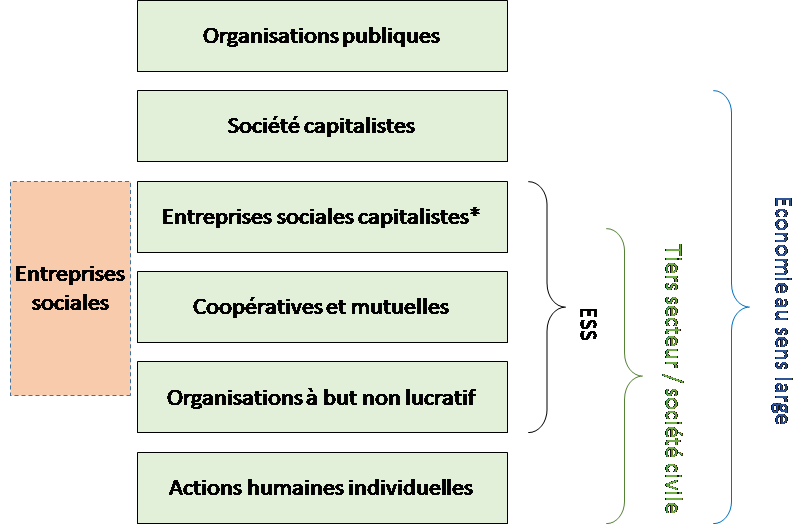
\includegraphics[width= 0.8\linewidth]{fig/tierssecteur.png}
                 \caption{L'ESS et le tiers-secteur}
                 \label{fig:tierssecteur}
             \end{figure}

            Si les auteurs ont salué la clarification apportée par \textcite{salamon2016beyond}, ils soulignent néanmoins que la question des frontières avec le secteur public et le marché n’est pas résolue et pose des problèmes d’opérationnalisation. En particulier, la question de la part des profits qui peut être distribuée reste à éclaircir \parencite{defourny2016voluntas}. Une autre critique de cette approche porte sur la terminologie, qui cantonne l’\ess à \cit{ce qu’il reste après l’État et le marché} et donc à négliger sa véritable place dans l’économie. L'\ess devient alors une composante de l"économie classique, une \citit{voiture balai} pour les personnes n'ayant pas trouvé leur place dans le système dominant \parencite{laville2011agir}. Cependant, un grand mérite de cette approche est d’être applicable au-delà des spécificités nationales et donc de rendre du compte du caractère universel de l’\ess \parencite{draperi2015leconomie}.


        \subsection{Un capitalisme social}

            L’ESS est souvent présentée comme une \cit{autre économie}, une \cit{économie alternative}, c’est-à-dire une alternative au système économique dominant. Elle s’inscrit alors dans une volonté de faire autrement, de proposer des schémas nouveaux qui remettent l’humain au cœur des activités économiques. Cependant, on observe un rapprochement récent entre l’\ess et le système capitaliste, faisant apparaître la première comme un fragment du système dominant qui adopterait une dimension sociale. Deux phénomènes mis en lumière dans la littérature nous semblent particulièrement bien éclairer cette évolution : l’émergence de l’entreprise sociale et la tendance croissante à l’adoption de logiques d’affaires dans l’ESS. \\

            L’entrepreneuriat social, concept issu du terrain, a donné lieu à une abondance de travaux au cours des dernières décennies. Il a donné naissance à plusieurs écoles adoptant des approches différentes du phénomène, allant des activités marchandes déployées par le secteur non lucratif jusqu’à l’intégration d’une mission sociale dans l’objet des sociétés capitalistes \parencite{defourny2011approches, petrella2014social}. L’école américaine des ressources marchandes met l’accent sur l’existence de ressources marchandes et de pratiques managériales issues du secteur privé classique. Les entreprises sociales sont d’abord définies comme des entreprises du secteur non lucratif qui déploient des activités économiques marchandes pour diversifier leurs sources de revenus. Une approche plus récente élargit le spectre à des entreprises à but lucratif dès lors que les ressources marchandes sont en partie mobilisées en vue d’une finalité sociale. Un cas particulier de cette école est celui du \textit{Social Business} popularisé par le prix Nobel de la paix Muhammad Yunus \parencite{yunus2010building, yunus2010building-1}. Ces entreprises ont une finalité sociale dont le coût est financé exclusivement par des ressources marchandes, selon la logique \citit{no profit, no loss}. Pour s’extraire du débat sur la lucrativité ou non des entreprises sociales,  l’école de l’Innovation Sociale se focalise non pas sur les ressources et leur usage, mais sur l’impact social et sur la nature de l’innovation qui génère cet impact. Cette logique est parfaitement résumée par le titre d’un article de \textcite{dees2003social} : \citit{Social Entrepreneurship is About Innovation and Impact, Not Income}. Au cœur de cette réflexion se situe l’entrepreneur (et non le collectif), moteur de l’innovation sociale. Enfin, \textcite{defourny2011approches} soulignent la spécificité de l’approche européenne, portée par l’EMES, qui s’appuie sur un idéal type basé sur neuf critères, relatifs aux dimensions économiques, sociales et de gouvernance de l’entreprise sociale. Les entreprises sociales ne sont donc pas définies strictement, mais doivent se rapprocher de cet idéal type. Dans la loi française, depuis 2014, le périmètre de l’ESS intègre des sociétés commerciales qui poursuivent une mission sociale. Elles doivent également respecter certaines règles de gestion portant sur la distribution des bénéfices, l’échelle des salaires ou encore la gouvernance et la démocratie d’entreprise. L’appartenance à l’ESS est formalisée par l’obtention d’un agrément (\esus). \\

            Un point commun des différentes approches de l’entreprise est de s’appuyer sur les schémas classiques de l’entreprise : que le profit soit possible ou non, les procédés managériaux et organisationnels sont ceux des entreprises capitalistes. Il ne s’agit pas du tout ici de remettre en cause le système dominant, mais au contraire de mobiliser ce qui a fait son succès, à savoir l’efficacité économique, pour résoudre les problèmes sociaux. Une forme d’économie sociale se développe donc au sein même du système économique dominant. Yunus propose ainsi un \citit{nouveau capitalisme}, c'est-à-dire un capitalisme qui ne serait pas orienté vers le profit mais vers une mission sociale, mais qui appliquerait les mêmes règles que le marché. Pour lui, les entreprises sociales sont en concurrence directe avec les entreprises de marché et doivent donc appliquer les mêmes règles et les mêmes modes de fonctionnement. Seule la finalité est différente. C’est la raison pour laquelle certains penseurs de l’ESS comme \textcite{draperi2015leconomie} contestent l’appartenance des entreprises sociales à l’ESS. \\

            Au-delà des entreprises sociales, l’ESS dans son ensemble est de plus en plus poussée à adopter un fonctionnement \citit{Business-like}  \parencite{dart2004being} qu’on pourrait traduire par \citit{ des logiques d’affaires}. Dans une récente revue de littérature, \textcite{maier2016nonprofit} recensent plusieurs raisons à ce phénomène déjà largement documenté, particulièrement pour le secteur non lucratif. Les premières raisons sont d’ordre stratégique et sont basées sur la rationalité économique. Faisant face à une concurrence croissante avec le secteur privé classique, ou au sein même de l’ESS, les entreprises cherchent à assurer leur indépendance et leur pérennité en s’appuyant sur des ressources de marché. Ceci est renforcé par la raréfaction des financements publics ou privés. En outre, les donateurs et partenaires privés ou publics, parties prenantes de la stratégie des entreprises de l’ESS, sont porteurs d’exigences en termes de performance et promeuvent l’application d’une logique d’affaires. Par ailleurs, ce changement est soutenu par la large prédominance de l’idéologie libérale au niveau international. S’inscrire dans ce système dont les codes sont omniprésents dans les sphères sociale, politique et économique devient un enjeu en termes de légitimité. Or celle-ci constitue une \citit{ressource opérationnelle} \parencite{suchman1995managing} et constitue un facteur indispensable de la pérennité des entreprises. La théorie institutionnelle souligne alors le rôle des isomorphismes : pour se légitimer, une entreprise cherche à ressembler à celles qui sont déjà légitimes, en reprenant les éléments qui les caractérisent, notamment les éléments symboliques comme les mythes, les symboles ou le vocabulaire \parencite{dimaggio2010iron, meyer1977institutionalized}. Or, comme le souligne \textcite{dart2004legitimacy}, le système économique basé sur le marché est devenu largement dominant, et donc plus légitime. L’ESS peut donc se légitimer en reproduisant ses pratiques :
            \begin{quotation}
                \citit{If business values, business models, and business language have become dominant and are the sociocultural environment’s preferred modes of problem solving and preferred structures of organizing, then it follows that even social-sector organizations can be accorded legitimacy by adopting the language, goals, and structures of this ideologically ascendant form.} (p.419)
            \end{quotation}

            En France, où l’ESS représente une part significative de l’économie et où le secteur associatif est fortement ancré, cette perspective d’un \cit{capitalisme social} est perceptible, comme l’illustrent quelques exemples symboliques. Le fondateur et dirigeant du plus grand groupe français d’économie sociale, Jean-Marc Borello a ainsi publié un ouvrage intitulé \citit{Pour un capitalisme d’intérêt général}. Plus récemment, le gouvernement a lancé \citit{l’initiative French Impact} qui vise à \citit{fédérer et valoriser la diversité des acteurs de l’innovation sociale} \parencite{ministere_de_leducation_nationale2018lancement}. L’ESS, ainsi intégrée dans un ensemble plus large autour d’un label et d’un objectif \cit{d’impact}, voit sa spécificité par rapport au reste de l’économie effacée. A tel point que le média Novethic suggère d’abonner l’expression \cit{économie sociale} au profit du \cit{French Impact} \parencite{alvarez2018ne}.

            Les études empiriques mettent en lumière des effets positifs de ces logiques d’affaires sur la performance et l’obtention de ressources humaines et financières. Elles semblent aussi aboutir à davantage d’innovations. Toutefois certains auteurs s’inquiètent de possibles dérives \parencite{maier2016nonprofit} et de la perte de l’identité des organisations \parencite[p. 134]{laville2016economie}. Le risque pour les entreprises est la focalisation sur la gestion et la performance, sur le marché et les clients, et la perte de vue des enjeux sociaux initialement adressés. Comment acquérir des ressources commerciales si les bénéficiaires initiaux sont justement insolvables ? La question se pose de l’équilibre entre les activités génératrices de ressources et les activités génératrice d’impact social.

            Pour certains auteurs, l’ESS est aussi porteuse d’une autre mission, celle de mettre la démocratie au cœur de l’économie. Or, l’économie néo-libérale serait précisément incompatible avec la démocratie \parencite{defalvard2016leconomie}. Ceci amène à une autre perspective de l’ESS, qui ne viserait pas seulement à résoudre des problèmes au niveau micro-économique, mais à porter un véritable changement de société.

        \subsection{Une économie transformatrice }

            Plusieurs auteurs dans le champ du management comme de l’économie politique ou de la sociologie soulignent le rôle politique de l’ESS et sa mission démocratique. Cette dimension fondatrice de l’économie sociale n’a pourtant pas toujours occupé une place centrale. La perspective historique  proposée par \textcite{chanial2002leconomie} permet de comprendre l’articulation entre économie sociale, économie solidaire et démocratie. Au \siecle{19} siècle, la charité est individuelle et elle est utilisée comme un outil de contrôle par le système libéral pour maintenir la paix sociale. Elle n’a pas de volonté d’émancipation des pauvres, mais vise au contraire à créer des liens de dépendance. A cette vision, les associations opposent une « solidarité démocratique » reposant sur l’action collective. Dans cette approche, la solidarité est réciproque, chacun ayant une dette envers la société. Pour \textcite{laville2016economie}, l’associationnisme redonne alors sa place à la démocratie à travers \citit{l’expérience sociale et l’inflexion des politiques publiques} (p. 74). Comme l’expliquent \textcite{chanial2002leconomie}, le \siecle{20} siècle est marqué par des législations qui viennent scinder l’économie sociale en associations, coopératives et mutuelles, rompant ainsi sa dynamique sectorielle. Les coopératives se sont ancrées dans des logiques de marché quand les mutuelles et associations ont adopté un rôle complémentaire par rapport à l’État. A partir des années 1960, à travers différents mouvements sociaux et face à l’incapacité de l’État à pallier les failles du marché, renaît une économie solidaire porteuse d’une vision transformatrice de la société. Des initiatives émergent qui \citit{mettent l’accent sur le modèle de développement et sur la participation citoyenne.} (p. 19). Alors que l’économie sociale repose sur les formes de propriété, l’économie solidaire valorise une économie plurielle, associant les mécanismes de marché, de réciprocité et de redistribution. Cette perspective trouve ses racines dans les travaux de Karl Polanyi \parencite{servet2007principe, polanyi1944great}, qui introduit le concept d'économie \cit{encastrée} dans les structures sociales. Pour lui, l'approche libérale qui cherche à extraire complètement le système économique des relations sociales est vouée à l'échec, et une économie autonome, désencastrée, ne pourrait aboutir qu'à la destruction de la société \parencite{block2003karl, valensi1980karl}. \\

            Pour \textcite{defalvard2016leconomie}, l'\ess doit jouer un rôle politique pour faire face aux dérives du néolibéralisme. Selon lui, ce système se distingue du libéralisme originel par l’absence de fondement éthique (seule compte l’efficacité), l’absence d’intérêt réciproque, puisque seul compte l’intérêt individuel, et la primauté de la finalité monétaire (par opposition à l’utilité des biens acquis). A cette \cit{théorie du marché}, s’oppose une \cit{théorie des communs}. Pour l’auteur, l’ESS se distingue donc par sa capacité à recréer du commun, à constituer une alternative économique \cit{en commun} au système néo-libéral. Ceci n’exclut nullement l’échange marchand, mais cet échange s’effectue dans un rapport au marché différent de celui du capitalisme, en ceci qu’il vise à renforcer le lien social plutôt qu’à le détruire, en adoptant un autre rapport au  développement et au territoire \parencite{draperi2015leconomie}.  Ainsi, pour \textcite[][p.64]{laville2016economie}, \citit{l’activité économique facilite l’émergence de l’expression politique} : elle permet aux individus de construire collectivement des solutions à leurs problèmes. L’ESS ne doit donc pas être vue seulement sous l’angle de l’économie capitaliste, mais aussi dans une perspective démocratique, comme le suggère \textcite{eikenberry2009refusing} :
            \begin{quotation}
                \citit{I suggest that, as an alternative to market-based discourse, nonprofit and voluntary organizations should focus their activities in a number of directions: on getting more people of diverse backgrounds to participate in organizational and societal governance, on making this participation meaningful in the sense of emphasizing relationships and engaging individuals “routinely in civic relationships over time” (Lichterman, 2006, p. 535), and on providing equal opportunities for members to participate in agenda setting, deliberation, and decision making.}
            \end{quotation}

            Pour l’auteure, ceci est incompatible avec une logique d’affaires, ancrée dans une logique d’intérêt individuel. Cette idée est partagée par \textcite{laville2011agir}, qui, s'appuyant sur les travaux d'Habermas, doute de la compabilité entre le capitalisme et la démocratie.
            En revanche, \textcite{dodge2016nonprofits} contestent la dimension a priori démocratique de l’ESS, ses organisations pouvant porter des pratiques et des valeurs contraires à celle de la démocratie. Sa place \citit{d’école de la démocratie} résulte nécessairement d’une démarche délibérée et active. Il convient donc d’écarter une vision idéaliste de l’ESS et des associations \parencite[][p. 26]{laville2016economie}. \textcite{mccambridge2004underestimating} insiste sur le rôle des organes de gouvernance des entreprises. Pour elle, l’ESS doit constituer un modèle de société et de démocratie. Elle a pour rôle d’amener les individus à participer à la vie civile et politique, rôle qui relève de la responsabilité du conseil d’administration. Ceci renvoie à un vaste champ de littérature sur la gouvernance de l’ESS et sur le rôle de cette instance \parencite{brown2010exploring, chait2005governance, collette2009economie, cornforth2004gouvernance, cornforth2012nonprofit, ostrower2006governance:, harrison2012perceptions}
             et les limites à l’application de la démocratie en son sein. En effet, l’égalité juridique des membres ne suffit pas à assurer un véritable fonctionnement démocratique, ni une véritable représentation des différentes parties prenantes \parencite[][p. 318]{laville2016economie}. Le rôle démocratique des \oess peut également s'exprimer directement à travers des actions de lobyying à destination du public (lobbyisme externe) ou bien des pouvoirs publics (lobbyisme interne) \parencite{junk2016two}. \\

            Si l’économie sociale renvoie aux statuts juridiques des entreprises et à leurs principes de fonctionnement, l’économie solidaire élargit le champ de l’ESS à \citit{des actions collectives à la fois socio-économiques et socio-politiques} \parencite[][p. 323]{laville2016economie}. L’auteur met ainsi en garde contre une définition trop restrictive de l’ESS qui s’appuierait sur les seules organisations constituantes. Ceci conduirait en effet à \citit{écarter les mouvements les plus significatifs de la période}, comme les circuits courts ou les monnaies locales \parencite{laville2017economie}. Ces dynamiques, en effet, ne sont pas la propriété ou l’initiative d’une entreprise, mais résultent d’une réorganisation de la vie en société sur un territoire qui implique des entreprises, des collectivités locales et des citoyens. C'est pourquoi l'auteur plaide pour élargir le champ de l'\ess aux actions individuelles ou hors cadre organisationnel, ainsi qu'à l'économie populaire. Celle-ci, particulièrement représentée dans les pays \cit{du Sud}, est directement liée à une logique de développement \parencite{ndiaye2011leconomie}. Les formes organisationnelles hybrides qui émergent au sein de l'économie populaire remettent en question la vision d'une \ess réparatrice, réduite à un rôle de compensation des maux causés par le capitalisme. Elles donnent au contraire l'image d'une économie émancipatrice qui permet aux populations les plus pauvres de se développer sans dépendre des systèmes économiques dominants. L'enjeu réside dans la consolidation du secteur et la reconnaissance de sa valeur par les observateurs et par les pouvoirs publics \parencite{larraechea2007leconomie}.

            \transition

            Nous avons décrit trois approches distinctes de l'ESS. Toutes sont porteuses d'une certaine vision de ce qu'elle est, mais aussi de ce qu'elle devrait être, selon les auteurs. Plutôt que de nous enfermer dans l'une de ces perspectives, au risque d'orienter les résultats de la recherche, nous mobilisons un concept capable de rendre compte des réalités diverses de l'ESS. Il s'agit de l'identité organisationnelle.

\section{L'identité organisationnelle}
    \subsection{Le concept d'identité}
        Qui sommes-nous en tant qu'organisation ? C'est la question à laquelle vise à répondre le concept d'identité organisationnelle, introduit par \textcite{albert1985organizational} et fréquemment mobilisé dans la littérature managériale. La définition proposée initialement par les auteurs, à savoir \citit{ce qui est central, persistant et distinctif dans le caractère d’une organisation}, fait l'objet d'une certaine confusion \parencite{chedotel2004ambivalence}. Par exemple, \citit{dans certains cas, l'identité organisationnelle est dépeinte comme une propriété subjective des observateurs, alors que dans d'autres cas, elle est décrite comme une propriété vérifiable des organisations} \parencite{whetten2006albert}. Le débat porte également sur le caractère malléable de l'identité : peut-elle être aisément manipulée par les dirigeants à des fins de communication ? Ceci a amené \textcite{whetten2006albert} à re-préciser le concept, en soulignant l'importance de ne pas se limiter à la question initiale pour son opérationnalisation. La première composante du concept est le caractère distinctif de l'organisation. Il vise à préciser de qui elle est similaire, et de qui elle est différente. Dans la mesure où l'organisation évolue dans un contexte économique et social, et où elle fait l'objet d'observations et de perceptions, elle doit appuyer son identité sur un discours, basé sur des catégories reconnues. Une organisation qui échoue à affirmer sa distinction risque d'apparaitre \citit{imprévisible et non digne de confiance} \parencite{whetten2006albert}. Pour l'auteur, l'aspect distinctif est inséparable du caractère \citit{central et durable} de l'identité, puisque c'est à travers un engagement réel et répété que l'organisation se distingue. Le caractère central correspond à ce qui est perçu comme essentiel dans l'organisation par ses membres. De la centralité découle la durabilité, puisque les éléments les plus fortement ancrés ont la plus grande probabilité de se maintenir dans le temps. \\


       \textcite{chedotel2004ambivalence} met l'accent sur le caractère ambivalent de l'identité organisationnelle. Alors que celle-ci est souvent perçue comme une caractérisation positive de l'organisation, l'auteur montre qu'une identité trop forte, comme une identité trop faible peuvent être dommageables. Une forte identité évite les situations d'ambiguïté ou d'incertitude, cependant elle limite la capacité d'évolution lorsqu'elle est trop fortement ancrée. A l'inverse, une identité faible, par manque de repères établis et consensuels, ouvre la voie à des conflits, voire à une incapacité à agir. \\

       L'identité organisationnelle a un apport intéressant pour l'étude de l'ESS qui peine à trouver une définition unique. Face à l'hétérogénéité des formes juridiques, il est souvent préféré une approche par ses caractéristiques distinctives, en particulier par les valeurs qu'elle met en avant \parencite{chedotel2004ambivalence}. Mais cette vision est également contestable, puisque l'\ess est aussi visée par une évolution managériale et adopte de manière croissante des logiques de marchés qui l'éloignent de ce positionnement purement normatif. Pour certains auteurs, des identités à première vue incompatibles peuvent en réalité coexister dans des organisations hybrides \parencite{chedotel2012linfluence, mariaux2018leconomie, foreman2002members}. Les \eess seraient-elles par essence des organisations de ce type ?


    \subsection{ESS et identité hybride}

        Tout comme les individus, les organisations peuvent associer de multiples identités qu'il est possible de contrôler \parencite{pratt2000classifying}. \textcite{foreman2002members} identifient des organisations hybrides associant une dimension normative et une dimension utilitariste. La dimension normative repose sur des traditions et des symboles, et met au centre une idéologie et une démarche altruiste. Les organisations ayant cette identité sont tournées vers la démocratie, la solidarité et la promotion sociale \parencite[][p.8]{chedotel2012linfluence}. La dimension utilitariste renvoie à l'intérêt personnel et à la rationalité économique. Les organisations s'inscrivent alors dans une logique de rentabilité et de pérennité. La coexistence de ces deux identités est observée dans des \oess comme les \scop, les mutuelles ou les banques coopératives par \textcite{chedotel2012linfluence}. Cette observation est partagée par \textcite{laville2016economie} qui identifie une dimension \cit{entreprise}, qui renvoie à l'approche gestionnaire de l'entreprise de l'\ess et une dimension \cit{mouvement}, qui correspond à sa vision transformatrice et à son rôle démocratique. Un conflit peut naître de la cohabitation entre une identité \cit{volontaire} et une identité \cit{managériale} dans les organisations ayant recours au bénévolat \parencite{kreutzer2011volunteering}. L'identité volontaire est celle à laquelle s'identifient les bénévoles. Elle est basée sur l'entraide et la générosité, et atteste du caractère solidaire de l'organisation. A l'inverse, les salariés mettent en avant le caractère professionnel à travers le respect des normes et procédures, ainsi que la rationalité économique de la gestion. D'autres exemples de structurations hybrides ressortent des travaux de Young sur le tiers secteur \parencite{young2001organizational, young2000alternative}. Les identités observées correspondent généralement aux mêmes dimensions normatives et utilitaristes. Toutefois, l'auteur identifie une identité dont l'élément central est l'efficacité dans l'atteinte des objectifs sociaux. \\

        Dans une précédente de recherche, portant sur un autre échantillon que celui utilisé pour la thèse, nous qualifions cette identité de \cit{fonctionnelle} \parencite{mariaux2018leconomie}. Cette étude porte sur la communication de 97 organisations de l'ESS sur leur site internet. Elle mobilise conjointement la théorie des parties prenantes \parencite{freeman1994politics, frooman1999stakeholder, laplume2008stakeholder} et le concept d'identité organisationnelle \parencite{scott2000stakeholder, sillince2009multiple}. Sur la base d'une analyse lexicale donnant lieux à plusieurs analyses factorielles des correspondances (AFC), cette recherche établit le lien entre les types de structures de l'ESS, les identités organisationnelles mies en avant, et les parties prenantes clés. Nous montrons ainsi que des identités peuvent être mobilisées différemment selon les parties prenantes qui sont perçues comme prépondérantes, ce qui met en évidence l'intérêt de l'hybridité de l'ESS. En effet, le management d'identités multiples donne à l'organisation une flexibilité et une capacité à s'adapter à des contextes et des interlocuteurs différents \parencite{pratt2000classifying}. Ainsi, les organisations s'adressant à leurs bénéficiaires (dans une perspective non marchande) mettent en avant l'identité fonctionnelle, en lien avec l'efficacité de leur action sociale. Celles qui s'adressent à des parties prenantes économiques (clients et fournisseurs) mettent l'accent sur l'identité utilitariste, mais aussi sur l'identité normative, soulignant les aspects \rse. Enfin, les entreprises ayant une gouvernance collective (particulièrement les mutuelles), mobilisent à la fois l'identité utilitariste (soulignant leur performance économique), l'identité normative (rappelant leur attachement aux valeurs), et l'identité fonctionnelle, tournée vers l'action sociale, activité principale des mutuelles \parencite{mariaux2018leconomie}. L'identité fonctionnelle est donc particulièrement mobilisée par les organisations lorsqu'elles s'adressent prioritairement aux bénéficiaires de leur activité (dans une perspective non marchande) ou bien aux parties prenantes impliquées dans la gouvernance. En effet, ces groupes de parties prenantes sont particulièrement intéressées par l'atteinte des objectifs concrets, plutôt que de savoir si l'organisation s'inscrit dans une perspective marchande, managériale, ou si elle met en avant des valeurs solidaires. \\

        L'existence d'identités multiples a cependant des effets plus négatifs. L'organisation fait face à des incitations contraires qui peuvent conduire à l'immobilisme ou à des conflits \parencite{pratt2000classifying}. Ces conflits s'expriment nettement dans l'\ess : selon l'identité normative, l'organisation devrait mener les actions les plus \cit{justes} ou les plus conformes à la volonté collective ; l'identité fonctionnelle pousse à choisir les actions qui ont le plus fort impact social ou environnemental ; et l'identité utilitariste encourage à choisir les actions qui ont le meilleur rapport entre la performance sociale et les coûts. La prépondérance d'une identité par rapport à une autre peut donc impacter les choix organisationnels. Alors que le courant entrepreneurial de l'\ess donne une place plus importante à la dimension utilitariste, certains auteurs s'inquiètent d'une possible \cit{dérive de la mission} \parencite[par exemple][]{ramus2017stakeholders, dart2004being, mair2012organizing}. \\

        Dans la section suivante, nous détaillons les éléments qui caractérisent les dimensions utilitariste, normative et fonctionnelle dans l'\ess et expliquons comment nous les mobilisons pour l'étude. Nous intégrons aussi une quatrième identité qui renvoie au caractère collectif, coopératif de ce segment de l'économie.

    \subsection{Quatre identités organisationnelles de l'\ess}

        La littérature rend compte du caractère souvent hybride des organisations de l'ESS, qui associent plusieurs identités d'apparence antinomiques. Quatre identités distinctes émergent fréquemment des travaux académiques (voir figure \ref{figure:dim_ess}). \\

        \begin{figure}
            \centering
            \caption{Identités organisationnelle des OESS}
            \label{figure:dim_ess}
            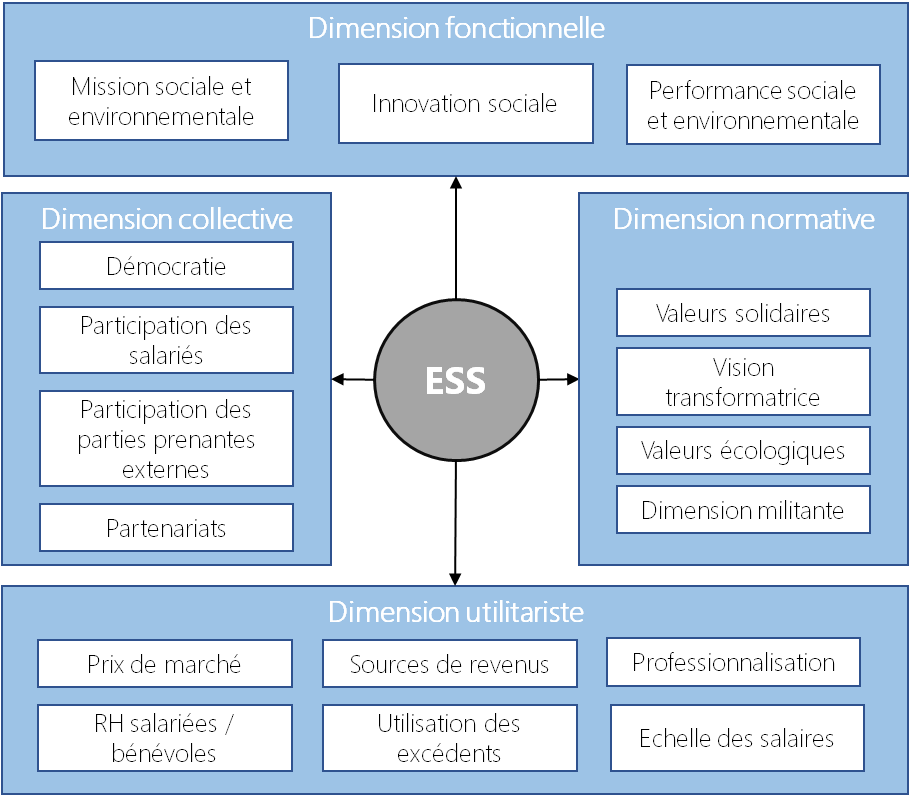
\includegraphics[width=\linewidth]{fig/dim_ess.png}
        \end{figure}

        \textbf{L'identité normative} fait écho au caractère \cit{social et solidaire} des \oess. Elle renvoie ainsi à la dimension socio-politique de l'ESS, par opposition à son rôle d'agent économique. \textcite[][p.293]{young2001organizational} parle d'une \citit{identité politique} qui vise à permettre la discussion et le débat, et éventuellement aboutir à une action collective.
        Malgré la forte hétérogénéité des organisations, le secteur pourrait ainsi se retrouver autour de valeurs ou de caractéristiques normatives. Une brève revue de littérature  de \textcite{mariaux2015leconomie} montre que l'\ess est présentée comme une économie différente, centrée sur l'humain, reposant sur la coopération entre les personnes et agissant pour l'intérêt général ou l'intérêt collectif et non pour des intérêts économiques ou personnels. \textcite{auger2014les} identifient des fondements normatifs importants dans des associations, comme la solidarité, la vie en communauté ou encore le respect. Mais elles soulignent que \citit{des valeurs plus austères sont évoquées}. \textcite{chedotel2004ambivalence} rappelle que cette vision peut être questionnée et qu'elle peut être vue comme un instrument de légitimation plutôt qu'une réelle identité de ses organisations. L'image d'entreprises responsables, agissant de manière éthique, aurait vocation à contrebalancer des scandales ou des cas de mauvaise gestion de structures de l'ESS. \\

       \textbf{L'identité utilitariste} s'inscrit dans l'approche gestionnaire de l'entreprise de l'ESS. \textcite{young2001organizational} la caractérise comme une \citit{identité économique}, qui traduit une volonté d'avoir un usage efficient des ressources au regard des objectifs à atteindre. \textcite[][p.840]{hansmann1980role} oppose ainsi des organisations \cit{commerciales} à des organisations reposant sur les dons (\citit{donative nonprofits}).
       L'identité utilitariste est adoptée par des organisations \citit{tournées vers le marché, orientées clients, auto-suffisantes, commerciales ou ayant une logique d’affaires} \parencite[][p. 414]{dart2004being}. Pour l'auteur, cette approche se caractérise par \citit{des objectifs exprimés en termes de générations de revenus, une organisation tournée vers le client, un fonctionnement managérial et une rhétorique commerciale} \parencite{dart2004legitimacy, mariaux2018leconomie}. Plusieurs auteurs observent et parfois s'inquiètent d'un mouvement généralisé de \cit{markétisation} ou de \cit{managérialisation}.  La tendance croissante des \eess à imiter le secteur lucratif \parencite{bidet2003insoutenable, valeau2013fonction} s'explique par une compétition croissante \parencite{dart2004being, frumkin2000when}, une volonté de légitimation (il est plus facile d'être reconnu lorsque l'on fait partie du système dominant et que l'on adopte ses codes) et une difficulté croissante à accéder aux financement dont ont besoin les organisations. En outre, il est intéressant de constater que l'approche de l'\ess par les valeurs (approche normative) - approche certes imparfaite, mais qui traçait une nette distinction avec le secteur lucratif - est progressivement remplacée par l'approche utilitariste, entrepreneuriale. Ainsi la loi cadre de 2014 caractérise l'\ess comme \citit{un mode d'entreprendre} \parencite{noauthor2014loi}, mettant ainsi en première place son rôle économique. \\

       Opérationnellement, l'identité utilitariste renvoie au mode de fonctionnement de l’entreprise : provenance des ressources (humaines et financières), adoption de prix de marché ou de prix adaptés à des situations spécifiques et possibilité de distribuer une partie des excédents. Ainsi, les entreprises ayant une forte identité utilitariste préfèrent le salariat au bénévolat et privilégient des ressources issues de leur activité à des dons et subventions. Elles déterminent les prix en fonction du marché et de la concurrence. A l'inverse, d'autres \oess proposent leurs produits gratuitement ou à moindre coût, ou au contraire à un prix plus élevé que le marché, mais considéré comme \cit{juste} (par exemple, les entreprises de commerce équitable). Enfin, certaines entreprises de l’\ess ont des statuts leur permettant de distribuer une partie des bénéfices réalisées. \\

        \textbf{L'identité fonctionnelle} de l'\ess ressort des travaux de \textcite{young2001organizational, young2000alternative} et \textcite{mariaux2018leconomie}. Les cas étudiés par \textcite[][p.292]{young2001organizational} mettent en lumière l'existence d'une identité qualifiée de \citit{goal-seeking systems} c'est-à-dire tournée avant tout vers la poursuite d'un but. Cette identité peut être rapprochée de l'analyse défendue par l'école de l'innovation sociale, pour qui l'efficacité sociale des \oess prime non seulement sur les aspects financiers mais aussi sur les valeurs \parencite{defourny2011approches}. Pour les auteurs, la question centrale est celle de l'utilité et l'innovation sociale \parencite{dees2003social}. Les questions gestionnaires ou normatives sont donc secondaires. Cependant, \textcite{auger2014les} soulignent le lien de cause à effet entre la dimension normative et la dimension fonctionnelle : ce sont souvent les valeurs personnelles, l'éthique et les convictions des managers qui façonnent la performance sociale et environnementale.  \\

        A notre connaissance, \textbf{la dimension collective} n'est pas identifiée comme une identité organisationnelle à proprement parler dans la littérature. Cependant, elle représente dans de nombreuses \oess un élément central et durable et constitue un caractère véritablement distinctif de l'ESS. Le critère de gouvernance démocratique, qui repose sur le principe \cit{une personne, une voix}, est ainsi inscrit dès l'article 1 de la loi de 2014 relative à l'ESS. Les statuts des organisations permettent d'intégrer à la gouvernance des parties prenantes multiples afin de mieux prendre en compte l'intérêt général dans les décisions. \textcite{petrella2014social} estiment par ailleurs que la place des entreprises sociales dans l'ESS dépend de leur capacité à s'organiser autour du caractère collectif et démocratique (p. 155). Une littérature abondante s'intéresse aux enjeux de la gestion du collectif dans les organisations de l'ESS, notamment du point de vue de la gouvernance et de l'intégration de multiples parties prenantes aux intérêts parfois convergents, parfois opposés. On peut ainsi distinguer des organisations \cit{mutuelles} (\citit{mutual nonprofit}), dont les dirigeants sont choisis par les membres et clients, et des organisations \cit{entrepreneuriales} dans lequelles la gouvernance fait l'objet d'un faible contrôle de la part des membres \parencite[][p.841]{hansmann1980role}. L'approche participative tient aussi une place importante dans la rhétorique des organisations, en particulier au sein des mouvements coopératifs et mutualistes qui sont nés d'une volonté d'agir en commun.

            \chapter*{Conclusion du chapitre \ref{chapitre:ess}}
                \addstarredchapter{Conclusion du chapitre \ref{chapitre:ess}}
                L'\ess n'est pas seulement le segment de l'économie qui regroupe les entreprises sociales, coopératives, associations, fondations et mutuelles. La littérature présentée dans ce chapitre dresse un tableau plus complexe, sans définition consensuelle, mais au contraire marqué par des disparités culturelles et idéologiques. Les auteurs l'appréhendent au sens large, à travers la notion de \cit{tiers secteur}, ou bien de manière plus restrictive en se limitant aux structures à but strictement non lucratif. Certains veulent en faire une composante sociale du système capitaliste, quand d'autres y voient une économie alternative. Elle est alternativement perçue comme porteuse d'une véritable dynamique entrepreneuriale, ou au contraire comme une voiture balai pour les laissés pour compte d'un système qui n'a pas une place pour chacun. L'émergence du concept d'entreprise sociale a bousculé l'ESS, et les tenants du système dominant accueillent positivement une économie sociale reposant sur des mécanismes de marché plutôt que sur la solidarité et la redistribution. Finalement réduite par la loi de 2014 à un \cit{mode d'entreprendre}, faisant face à une baisse massive des financements publics, mais aussi des dons privés, il se pose la question du rôle que l'\ess tiendra face aux enjeux de demain. \\

L'incertitude sur l'\ess interroge son identité. Les auteurs relèvent le caractère hybride de cette économie qui associe plusieurs \citit{vocations} organisationnelles, plusieurs identités. La thèse se propose d'analyser l'\ess sous le spectre de quatre identités. L'identité utilitariste renvoie à la recherche de rentabilité et à l'adoption de modalités de gestion managériales qui la rapproche de l'économie classique. Parfois critiquée pour le tableau idéaliste qu'elle dépeint, l'identité normative témoigne de la place de l'éthique, des valeurs et d'une démarche solidaire et humaniste dans l'ESS. La dimension fonctionnelle s'intéresse à la fin plutôt qu'aux moyens, et renvoie à sa mission sociale ou environnementale, et à la recherche d'impact concret sur les publics bénéficiaires de l'action des \oess. Enfin, l'identité collective renvoie à la démarche historique de mise en commun et de mutualisation des outils de production. Elle traduit la volonté de \cit{faire ensemble}, plutôt que d'agir comme des agents économiques désencastrés de la sphère sociale. Le recours à ce cadre théorique offre l'avantage d'échapper à une vision simpliste, ignorant les importantes variations parmi des organisations au même statut juridique. \\


            \chapter{Prise en compte de l'environnement dans les organisations : du discours aux actes}
                \label{chapitre:ei}
                \minitoc \newpage
                % !TEX root = /Admin/main.tex

\section*{Introduction du chapitre}

La protection de l'environnement est devenue aujourd'hui un enjeu majeur - et pressant - pour la société. On voit se produire des changements organisationnels, comme l'introduction des rapports RSE parallèlement aux rapports annuels ; sociaux (tel que le mouvement des étudiants pour le climat en 2019) ; ou politiques, avec les bons succès électoraux de partis écologistes lors d'élections récentes. La communauté scientifique s'inscrit dans ce mouvement, comme le traduit une forte croissance du nombre de publications sur l'innovation environnementale depuis 2009 \parencite{diaz-garcia2015eco-innovation:}. Ce chapitre a pour objectif de montrer comment la littérature appréhende la prise en compte de l'écologie dans les organisations. De manière un peu surprenante, les recherches s'intéressent d'abord à la divulgation environnementale (à partir des années 1980, selon \textcite{ali2017determinants}), avant de porter davantage d'attention à l'innovation. \\

La divulgation environnementale désigne la communication des entreprises sur leur impact environnemental et sur les actions entreprises pour le réduire. Il s'agit d'une communication essentiellement formelle, s'inscrivant dans le cadre des documents de référence ou prenant la forme de communiqués de presse. Dans une première section de ce chapitre, nous présentons une synthèse de l'état de l'art, en soulignant notamment ses déterminants et ses effets. L'information donnée n'est jamais neutre : elle a pour objectif de répondre aux attentes et aux interrogations de différentes parties prenantes, et de convaincre de la pertinence et de la validité de l'activité de l'entreprise. Elle vise aussi à démontrer la conformité aux réglementations en vigueur. Or, les attentes et les réglementations sont multiples et peuvent paraître contraires aux intérêts des organisations. L'utilisation du langage, de la rhétorique, devient un outil pour répondre à ces attentes. Nous faisons le lien avec le chapitre \ref{chapitre:ess} en soulignant le rôle de l'identité organisationnelle dans les stratégies rhétoriques. La notion de cadrage rhétorique est également présentée. La typologie de \textcite{nisbet2010framing, nisbet2009communicating}, qui applique le cadrage au débat environnemental, est utilisée comme outil d'analyse pour la partie empirique de la thèse (chapitre \ref{chapitre:twitter}). \\

L'étude de la communication conduit à se questionner sur les actions réelles des organisations. La deuxième section du chapitre propose d'y répondre à travers le concept d'innovation environnementale, ou éco-innovation (EI). Depuis quelques années, les chercheurs s'évertuent à montrer ce qui motive le développement d'innovations prenant en compte l'environnement. Les motivations sont de trois ordres \parencite{bansal2000why}. Elles répondent d'abord à une recherche de compétitivité, indispensable à la survie des entreprises. Souvent présentée comme une contrainte pour les entreprises, l'écologie peut pourtant contribuer à les rendre plus efficientes. La recherche de légitimité, de conformité et de satisfaction des parties prenantes est un second facteur influençant l'éco-innovation. Enfin, les valeurs portées par les membres des organisations, en particulier le top-management, influencent les stratégies d'innovation environnementale. La littérature souligne aussi la variété des innovations, qui ne sont pas seulement des nouvelles technologies, mais résident aussi dans les changements d'organisation, de comportements individuels, ou dans l'organisation de nouvelles pratiques au niveau d'une industrie ou d'un réseau d'acteurs. \\

Enfin, le chapitre se termine sur le lien entre l'action environnementale et les caractéristiques des \oess. La littérature est peu abondante sur ce point. L'étude de l'éco-innovation ou de la divulgation concerne généralement les entreprises classiques, quand l'étude de l'\ess s'intéresse plus généralement à la gouvernance ou à l'action sociale. Pourtant, des auteurs soulignent l'importance d'interroger la place des questions environnementales dans l'\ess \parencite{dart2010green, buchs2014role, edwards2013environmental}. Si en premier lieu, ce segment de l'économie semble mieux à même de répondre à l'urgence environnementale que le secteur privé classique, il fait néanmoins face à de nombreux obstacles.

\section{La communication environnementale}

    Dans cette section, nous nous intéressons à la façon dont les entreprises abordent les questions environnementales dans le discours et la communication institutionnelle. Dans un premier temps, nous nous consacrons à la divulgation environnementale, c'est-à-dire aux éléments communiqués par les entreprises sur leur action. Dans un second temps, nous nous penchons sur les stratégies rhétoriques qui peuvent être mobilisées dans la communication.

    \subsection{La divulgation environnementale des entreprises}

        L'intérêt croissant pour la \rse s'est accompagné d'une communication plus importante des entreprises sur leur impact environnemental. Face à la montée des attentes des parties prenantes et à la crainte de voir émerger des régulations plus contraignantes, de nombreuses entreprises publient pro-activement des informations environnementales sur leur activité \parencite{cormier2007revisited, cormier1999corporate}. De nombreuses recherches visent à identifier précisément les facteurs qui motivent la divulgation volontaire et à en mesurer les effets. Les auteurs étudient notamment le lien entre la divulgation et la performance économique (croissance de la part de marché, du chiffre d'affaire ou de la rentabilité), la réaction des consommateurs et des actionnaires, considérés comme les parties prenantes les plus importantes, et l'effet en termes de légitimité et d'impact médiatique. Les résultats se révèlent toutefois inconsistants et parfois contradictoires \parencite{gray2001social}. En outre, des effets opposés sont parfois observés d'un pays à l'autre \parencite{bouten2012how, cormier2007revisited}.

        \subsubsection{Déterminants de la divulgation}
            Un certain nombre de recherches étudient les déterminants du niveau de divulgation environnementale des entreprises. Elles cherchent à identifier les caractéristiques des entreprises qui expliquent la quantité et la qualité de l'information communiquée sur l'impact environnemental, généralement sous la forme de communiqués ou dans les rapports annuels. \textcite{bouten2012how} soulignent l'importance de distinguer le choix de divulguer ou non, et le niveau de divulgation. Ainsi les facteurs qui décident une entreprise de communiquer sur les pratiques environnementales et du volume d'information à divulguer diffèrent. \\

            Un facteur régulièrement relevé est la taille de l'entreprise \parencite{cormier1999corporate}, qui impacte la décision de divulguer \parencite{bouten2012how}. De nombreux facteurs financiers sont également identifiés comme déterminants de la divulgation : la situation financière de l'entreprise \parencite{cormier1999corporate}, le levier (soit le ratio dette sur capital), la dispersion du capital , le niveau de risque et le ROE \parencite{bouten2012how}. \textcite{da_silva_monteiro2010determinants} soulignent également que le fait d'être cotées en bourse impacte significativement le niveau de divulgation des entreprises portugaises. Les auteurs relèvent aussi l'impact du coût de l'information \parencite{cormier2004impact} et de l'exposition médiatique \parencite{bouten2012how}. Les entreprises agissant dans un domaine sensible du point de vue environnemental divulguent davantage d'informations que les autres \parencite{aerts2008corporate, radhouane2018customer-related}.


            % \todo[inline]{On pourrait citer aussi Cho  and  Patten,  2007;  Clarkson  et  al.,  2008;  Liu  and  Anbumozhi,  2009}


        \subsubsection{Effets de la divulgation environnementale}

            La littérature s'intéresse à l'impact de la divulgation environnementale sur la performance économique, la légitimité organisationnelle et sur  la performance environnementale. \\

            L'effet de la divulgation environnementale sur la performance présente un intérêt évident pour les partie prenantes, en particulier pour les actionnaires, et fait naturellement l'objet de nombreuses études. \textcite{cormier2007revisited} mesurent un effet du reporting environnemental sur le coût du capital mais les différents éléments divulgués n'ont pas le même effet. En outre, le contexte de l'entreprise influence également l'effet de la divulgation. Plusieurs études trouvent un effet positif de la divulgation sur la valeur de marché \parencite{radhouane2018customer-related, cormier2015does, plumlee2015voluntary, aerts2008corporate}. Cependant, les actionnaires prennent également en compte le coût supporté dans leur évaluation de la divulgation. Ce coût est perçu comme plus élevé dans les industries sensibles sur le plan environnemental, car la divulgation peut entraîner une réaction de parties prenantes, voire conduire à de nouvelles législations contraignantes \parencite{radhouane2018customer-related}. \\

            Bien qu'elle apparaisse plus abstraite, la littérature abondante sur la légitimité organisationnelle semble valider l'assertion de \textcite{suchman1995managing} qui la présente comme une \citit{ressource opérationnelle}, essentielle à la pérennité d'une entreprise.
            Le niveau de légitimité est impacté positivement par une divulgation environnementale réactive, en réponse à une situation particulière, mais non par une communication pro-active. Le volume et la qualité des éléments économiques de la communication environnementale sont également déterminants pour la légitimité \parencite{aerts2008corporate}. Pour \textcite{brammer2008factors}, les grandes entreprises, ainsi que celles qui sont directement concernées par des questions environnementales présentent une information de meilleure qualité.

            Alors que la littérature tend à séparer les incitations financières et les incitations en termes de légitimité sur la divulgation environnementale, \textcite{cormier2015economic} soulignent leur interdépendance. Ainsi, les décisions relatives à la divulgation  doivent être prises en considération de multiples parties prenantes, incluant aussi bien les partenaires financiers que les médias et le public. Pour les auteurs, les efforts de communication sur les actions environnementales sont nécessaires car leur absence aboutit à \citit{une perte de crédibilité ou de réputation} (p. 17). La divulgation bénéficie aux parties prenantes financières mais permet aussi d'établir un meilleur dialogue avec la société civile et les pouvoirs publics. \\

            Outre les effets sur la performance économique et la légitimité des entreprises, la divulgation aboutit-elle à une meilleure performance environnementale ? \textcite{vazquez2008corporate} trouvent une forte relation entre le discours organisationnel et la performance environnementale. Toutefois, la littérature souligne l'importe d'une véritable culture d'entreprise pour améliorer la performance \parencite{crane2017rhetoric}. \textcite{al-tuwaijri2003relations} constatent que les entreprises qui ont la meilleure performance environnementale divulguent davantage d'informations environnementales. Évidemment, la divulgation est ici une conséquence de la performance, puisque l'incitation est forte à communiquer sur des \citit{bonnes nouvelles}. Cependant, les auteurs identifient aussi un lien de cause à effet entre la divulgation passée et la performance environnementale actuelle. La communication passée établit un seuil minimum de performance environnementale que l'organisation doit maintenir, au risque de décevoir les parties prenantes dont les attentes s'alignent sur les résultats passés.


    \subsection{Rhétorique et cadrage du discours}

        Le langage utilisé tient un rôle essentiel dans la communication environnementale des entreprises. La recherche en management s'appuie sur la rhétorique pour mettre en lumière les mécanismes mobilisées par les organisations. L'étude de la rhétorique remonte à l'antiquité Grecque, et aux écrits d'Aristote \parencite{aristotle1991rhetorique}, qui servent encore de base à son étude \parencite[par exemple][]{waldron2016how, brennan2014rhetoric, green2004rhetorical}. Pour plusieurs auteurs, la rhétorique est étroitement liée avec l'identité organisationnelle \parencite{sillince2009multiple, waldron2016how, frandsen2011rhetoric}. Dans cette section, nous discutons des mécanismes rhétoriques utilisés pour présenter l'action environnementale, en lien avec l'identité organisationnelle.


        \subsubsection{Définition et rôle de la rhétorique}
           \textcite{brennan2014rhetoric} définissent la rhétorique comme \citit{les ressources de communication utilisée pour atteindre des objectifs donnés}. Elle a cependant une intention de persuasion qui la distingue du simple \cit{discours} \parencite{higgins2012ethos}.

            La rhétorique est essentielle dans les organisations. Elle sert non seulement à échanger de l'information, mais aussi à construire une réalité sociale et organisationnelle \parencite[][]{heracleous2001organizational}. C'est ainsi par le discours qu'est créée la valeur perçue des innovations, ce qui en facilite la diffusion \parencite{green2004rhetorical}. \textcite{sillince2009multiple} démontrent que la rhétorique contribue à la création d'un avantage compétitif. En s'appuyant sur l'identité organisationnelle, elle donne aux ressources un caractère rare, non imitable et non substituable. Pour \textcite{heath2011external}, le discours des organisations a pour but de \citit{co-créer la réalité avec les publics extérieurs nécessaire pour obtenir un alignement d'intérêt plutôt que de souffrir de frictions nocives}. C'est aussi par la rhétorique que les organisations peuvent mobiliser les parties prenantes et obtenir leur adhésion, voire leur soutien \parencite{waldron2016how, brennan2014rhetoric}. Elle permet aussi de mobiliser l'engagement public face à des enjeux sociétaux et politiques, comme le réchauffement climatique \parencite{nisbet2009communicating}.

            Health souligne la distinction entre la rhétorique interne, instrument du lien entre l'organisation et les individus qui la composent, et la rhétorique externe, qui établit un pont avec la société.

        \subsubsection{Les preuves rhétoriques d'Aristote}
            Selon le philosophe, les rhéteurs s'appuient sur le \citit{logos}, c'est-à-dire la raison (apparente) et la démonstration scientifique, le \citit{pathos}, qui joue sur les émotions et les sentiments, et l'\citit{éthos}, qui met en avant le caractère moral et la crédibilité \parencite{higgins2012ethos}. Le \textit{logos} s'appuie sur l'argumentation, la logique, les justifications et preuves, les données ainsi que des exemples historiques. Le \textit{pathos} prend la forme de métaphores et d'identification à l'aide de références culturelles (sport, richesse, loyauté, amitié...). Enfin l'\textit{ethos} permet de construire la crédibilité en s'appuyant sur la similarité, la déférence, l'expertise, l'auto-critique, la volonté de réussir et la consistence \parencite[][p.198]{higgins2012ethos}. Pour ces auteurs, les trois registres sont mobilisés dans la communication environnementale des entreprises, cependant l'un prédomine généralement sur les autres. En outre, ils sont utilisés dans la construction de l'identité organisationnelle. Dans les cas étudiés par les auteurs, l'\textit{ethos} appuie l'identité d'une \citit{credible persona} (p.205), le \textit{pathos} souligne l'identité d'un \cit{bienfaiteur paternaliste} (p.201) et le logos, appuyé par les deux autres, confère l'identité d'une \cit{bonne entreprise citoyenne} (p. 204). \\

            \textcite{waldron2016how} font quant à eux le lien avec le différentiel d'identité entre l'organisation à l'origine du discours et celle qui en est destinataire. Lorsque ce différentiel est faible, des arguments rationnels, factuels, sont préférés (\textit{logos}), car ils vont vraisemblablement être compris par un interlocuteur proche de l'émetteur. Mais si le différentiel est fort et que les raisons factuelles de l'organisation risquent de ne pas être entendues par le destinataire du discours, l'organisation a recourt à des arguments basés sur le registre dramatique ou moral (\textit{pathos}). \\

            Le discours ne doit pas s'appuyer sur un seul de ces leviers, au risque de ne retenir l'attention que d'une partie de l'audience. \textcite[][p.14]{nisbet2009communicating} met en évidence cet effet dans le débat environnemental :
            \begin{quotation}
                \citit{De nombreux scientifiques et défenseurs [du climat] s'attendaient à ce que cette attention accrue des médias favorise une meilleure compréhension de la nature technique du problème par le grand public [...].  La communication est donc définie comme un processus de transmission, c'est-à-dire que les faits scientifiques sont censés parler d'eux-mêmes, leur pertinence et leur importance politique étant interprétées par tous les publics de la même manière. Malheureusement, une couverture médiatique de qualité n'atteindra probablement qu'un petit public de citoyens déjà informés et engagés.}
            \end{quotation}

        \subsubsection{Cadrage du discours}
            \citit{Les cadres sont des scénarios d'interprétation qui déclenchent un train de pensée précis, expliquant pourquoi une question pourrait soulever un problème, ce qui pourrait en être responsable, et ce qui devrait être fait pour y remédier} \parencite[][p.15]{nisbet2009communicating}. Le cadrage consiste ainsi à inscrire le discours dans un contexte qui va permettre d'en créer le sens. Tout discours, quel qu'il soit, s'inscrit nécessairement dans un cadre donné \parencite{nisbet2009communicating}. Le discours peut mobiliser différents cadres en fonction de l'objectif à atteindre. Par exemple, \citit{Poser un problème tel que la pollution dans le langage du discours dominant est un moyen puissant de présenter un argument et d'influencer l'opinion, puisque le discours dominant n'a pas besoin d'explications étendues ou de légitimation, car il est familier, reconnaissable, et accepté par une variété d'audiences} \parencite[][p.598]{mcgregor2004sustainable}. Pour \textcite{feinberg2013moral}, la polarisation du débat environnemental relève en grande partie du caractère moral qui lui est donné. Une échappatoire à cette polarisation consiste à inscrire ce débat dans une cadre différent, moins clivant.

            \textcite{waldron2016how} indiquent que l'identité guide l'utilisation des cadres rhétoriques. Plus précisément, c'est le différentiel d'identité perçu avec les entreprises visées par le discours qui est important pour les auteurs. Les entrepreneurs sociaux qui perçoivent un faible différentiel d'identité avec leur interlocuteur adoptent une stratégie isomorphique, mobilisant les cadres de référence de celui-ci. Mais en cas de fort différentiel d'identité, les entrepreneurs sociaux s'appuient sur des cadres différents, afin de pousser l'interlocuteur à faire évoluer sa position. \\

            Les questions environnementales, qui font l'objet d'un débat important dans la société, et se révèlent fortement polarisantes \parencite{nisbet2009communicating}, n'échappent pas à ce besoin de cadrage. \textcite{gamson1989media} étudient les cadres mobilisés lors du développement de l'énergie nucléaire. Les promoteurs de cette industrie faisaient passer le message d'une innovation très positive : \citit{Atoms for peace. Your friend, the atom. Electricity too cheap to meter.} \parencite[][p.1]{gamson1989media}. Plus généralement, les auteurs mettent en lumière sept cadrages du discours : le progrès, l'indépendance énergétique, le \cit{marchandage avec le diable} (\textit{Devil's bargain}), le \cit{sauve-qui-peut} (\textit{runaway}), la responsabilité publique, la non-rentabilité et les chemins alternatifs (\textit{soft paths}). Plus récemment, \textcite{nisbet2009communicating, nisbet2010framing} étend cette typologie et l'applique au cas du réchauffement climatique. Il aboutit à neuf cadres fréquemment utilisés dans le débat scientifique et sociétal (tableau \ref{table:typonisbet}).

            \begin{table}[h]
                \caption{Typologie de cadres applicables à la question du climat}
                \label{table:typonisbet}
                \begin{tabularx}{\linewidth}{|K{0.30\textwidth}|X|}

                    \hline
                    \textbf{Cadre} & \textbf{Les cadres définissent le problème posé comme...} \\ \hline
                    \hline
                    Progrès Social
                    & l'amélioration de la qualité de vie ou la résolution de problèmes. Alternativement, comme une harmonie avec la nature plutôt que sa maîtrise, la durabilité
                    \\ \hline

                    Développement économique et compétitivité
                    & les investissements économiques, les avantages ou les risques du marché ; la compétitivité à l'échelle locale, nationale ou globale.
                    \\ \hline

                    Moralité et éthique
                    & en termes de bien ou de mal ; respecter ou franchir des limites, des seuils ou des limites
                    \\ \hline

                    Incertitude scientifique et technique
                    & une question de compréhension par les experts ; ce qui est connu par opposition à ce qui est inconnu ; invoque ou au contraire met en doute le consensus des experts et fait appel à l'autorité des sciences dures, à la falsifiabilité ou à l'examen par les pairs
                    \\ \hline

                    Boîte de Pandore, Monstre de Frankenstein et \cit{Sauve-qui-peut}
                    & un appel à la précaution face à d'éventuels impacts ou catastrophes. Hors de contrôle, un monstre de Frankenstein, ou un fatalisme, c'est-à-dire que l'action est futile, le chemin est choisi, pas de retour en arrière possible.
                    \\ \hline

                    Responsabilité publique et gouvernance
                    & une recherche dans l'intérêt public ou au service d'intérêts privés ; une question de propriété, de contrôle ou de brevetage de la recherche, ou une utilisation responsable ou un abus de la science dans le processus décisionnel ; la \cit{politisation}
                    \\ \hline

                    Alternatives et compromis
                    & autour de la recherche d'une position de compromis possible, ou d'une troisième voie entre des points de vue ou des options conflictuels ou polarisés.
                    \\ \hline

                    Conflits et stratégies
                    & comme un jeu entre élites ; qui est en avance ou en retard pour gagner le débat ; bataille de personnalités ; ou de groupes ; (généralement l'interprétation est dirigée par les journalistes)
                    \\ \hline
                \end{tabularx}
                \footnotesize{Source : \textcite{nisbet2010framing}}
            \end{table}


        \subsubsection{Le discours du \cit{juste milieu}}
            \textcite{higgins2012ethos} montrent comment la rhétorique est mobilisée par les entreprises pour mettre en place une stratégie de \citit{juste milieu} (\textit{middle ground}) qui consiste à l'imbrication des questions environnementales dans les aspects économiques. Ce rapprochement est fait sans égards pour les frictions qui en résultent et sans mention de l'incapacité du marché à répondre aux enjeux environnementaux \parencite{livesey2002discourse}. Ainsi, \textcite{laine2005meanings} estime que le langage de la divulgation environnementale vise à créer la vision d'une démarche \cit{gagnant-gagnant}, associant performance environnementale et progrès économique. Ceci permet aux entreprises de se maintenir dans le discours dominant, celui du libre-marché, tout en répondant aux injonctions des défenseurs de l'environnement. Le discours mobilise le cadrage de l'effet positif du développement économique sur les questions sociales et environnementales \parencite{livesey2002discourse}. Des thématiques devenues récurrentes et communément acceptées sont ainsi au service de ce discours, comme la notion de \citit{triple bottom line} \parencite{higgins2012ethos}. \textcite{milne2006creating} soulignent aussi la prépondérance de la métaphore du \cit{voyage} vers des pratiques durables. Elle permet de donner l'impression d'une démarche active et confère une vision optimiste de l'avenir, permettant d'obtenir l'approbation du public. Elle est aussi utilisée pour \citit{redéfinir le développement durable dans des termes qui ne menacent pas le 'business as usual'}. \\

            Cette recherche d'un juste milieu a en réalité pour objectif de maintenir les pratiques économiques habituelles et de réduire les pressions exercées par les partisans de l'écologie. Elle est à rapprocher du management des impressions (\citit{impression management}) \parencite{cho2010language, frandsen2011rhetoric, higgins2012ethos} qui désigne \citit{le processus par lequel les individus s'efforcent de contrôler les impressions que les autres forment sur eux} \parencite[][p.34]{leary1990impression}. En gestion des organisations, il est utilisé pour obtenir des bénéfices matériels et sociaux, et créer une identité désirable \parencite{merkl-davies2007discretionary}. D'après \textcite{cho2010language}, la divulgation environnementale constitue elle-même un outil de management des impressions.

            \transition

            Les stratégies des entreprises pour répondre aux attentes environnementales tout en maintenant leur pratique et leur rentabilité soulèvent des questions intéressantes dès lors que l'on s'intéresse à l'ESS. En effet, nous avons vu que dans sa définition cette économie donne la priorité aux conséquences sociales et environnementales de leur action. Cependant, la tendance entrepreneuriale du secteur peut aussi les conduire à adopter ces mêmes pratiques de communication et de construction des impressions.


\transition

    Dans cette section, nous avons discuté de la communication environnementale des entreprises. Au delà des écrits et des paroles, ce sont les actions concrètes qui peuvent avoir un impact sur l'environnement. Or, avec la progression importante des pratiques de \rse, il peut s'avérer difficile de déterminer si une entreprise agit réellement de manière éco-responsable ou si elle se contente de pratiquer un \citit{green-washing} \parencite{parguel2011how}. Ainsi, \textcite{cho2010language} vérifient bien que les entreprises les moins performantes du point de vue écologique divulguent l'information environnementale de manière plus optimiste et plus assurée que les plus performantes. En s'appuyant sur la théorie institutionnelle, des auteurs argumentent toutefois que les entreprises sont susceptibles de devenir demain ce qu'elles prétendent être aujourd'hui, et donc d'appliquer réellement les bonnes pratiques environnementales qu'elles mettent en avant dans la communication \parencite{frandsen2011rhetoric}.

    Dans la section suivante, nous laissons de côté les discours, pour nous intéresser plutôt aux pratiques, à travers le concept d'\ei.


\section{L'éco-innovation : une démarche éthique ou pragmatique ?}



    L'innovation est depuis longtemps un élément important de la littérature économique et managériale. Selon \textcite{schumpeter2006capitalism}, le capitalisme est par essence un système dynamique, évolutif. La capacité des entreprises à changer pour s’adapter à ces évolutions, à travers un processus de \citit{destruction créatrice}, est donc une clé de leur réussite. Pour certains auteurs, l’innovation est un moyen d’obtenir des avantages compétitifs leur permettant de faire durablement face à la concurrence (McDonald, 2007). Il n’est donc pas étonnant qu’elle soit au cœur de nombreuses recherches. Une définition communément retenue est celle de l’OCDE \parencite{oecd2005oslo} :
    \begin{quotation}
        \citit{The implementation of a new or significantly improved product (good or service), or process, a new marketing method, or a new organisational method in business practices, workplace organisation or external relations. }
    \end{quotation}

    L’innovation est distincte de l’invention, qui n’est que l’émergence d’une idée ou d’une technologie nouvelle. Celle-ci ne peut être qualifiée d’innovation que dès lors qu’elle est introduite sur un marché. \textcite{baregheh2009towards} comparent 60 définitions distinctes dans des revues en management, innovation, organisations, technologies ou marketing. Ces définitions insistent sur la nature de l’innovation (la nouveauté), ses typologies, ses objectifs, le contexte social dans lequel elle s’applique, les moyens nécessaires à sa mise en place et les étapes respectives. A partir de la synthèse de ces différentes approches, les auteurs proposent la définition suivante :
        \begin{quotation}
            \citit{Innovation is the multi-stage process whereby organizations transform ideas into new/improved products, service or processes, in order to advance, compete and differentiate themselves successfully in their marketplace.}
        \end{quotation}

    L’essence de l’innovation repose dans son caractère nouveau, dans le changement qu’elle induit par rapport à une situation précédente. Pour \textcite{johannessen2001innovation}, l’innovation peut être appréhendée par un \citit{dénominateur commun} : la nouveauté. Leurs résultats montrent que l’innovation est un concept unidimensionnel caractérisé uniquement par le degré de radicalité. On distingue donc les innovations incrémentales des innovations radicales. Les innovations incrémentales concernent des modifications continues et graduelles qui ajoutent de la valeur tout en maintenant le processus de production existant, alors que les innovations radicales créent une discontinuité et visent à remplacer l’existant \parencite{carrillo-hermosilla2010diversity}. Il faut toutefois souligner que la nouveauté, et donc l’innovation, sont des perceptions et dépendent du point de vue duquel on se place, ou de \citit{l’unité d’adoption pertinente} \parencite{johannessen2001innovation}. Selon l'\textcite{oecd2015innovation}, \citit{une innovation peut être nouvelle pour l’entreprise, pour le marché, ou pour le monde}. Ainsi, ce qui peut constituer une innovation importante pour l’organisation n’est pas nécessairement perçu comme tel par les consommateurs.  Il est donc important, lorsqu’on cherche à étudier l’innovation, de spécifier le cadre dans lequel on l’analyse. \\



    Le terme d’innovation évoque souvent l’émergence de nouvelles technologies. Pourtant, le concept englobe un champ beaucoup plus large. Déjà en 1942, dans son ouvrage de référence \cit{Capitalisme, Socialisme et démocratie}, \textcite[][p.83]{schumpeter2006capitalism} intègre les nouveaux produits, les nouvelles méthodes de production ou de transport, les nouveaux marchés, les nouvelles formes d’organisation industrielle créées par l’entreprise capitaliste (son propos portant spécifiquement sur ce système). L’OCDE distingue quatre principales catégories d’innovation : l’innovation produit, process, marketing ou organisationnelle (cf. encadré \ref{encadre:typoinnov}). \\

    \begin{encadre}
        \begin{tcolorbox}
        \caption{Typologie d'innovations}
        \label{encadre:typoinnov}
            \textbf{  Innovation produit} : l’introduction d’un bien ou service nouveau ou significativement amélioré dans ses caractéristiques ou son usage attendu. Ceci inclue les améliorations signataires des spécifications techniques, composants et matériaux, logiciels incorporés, interface utilisateur ou autres fonctions techniques. \\

            \textbf{ Innovation process} : l’implémentation d’une méthode de production ou de délivrance nouvelle ou significativement améliorée. Ceci inclue des changements significatifs en matière de techniques, d’équipements et/ou de logiciels. \\

            \textbf{ Innovation marketing} : l’implémentation d’une nouvelle méthode marketing impliquant un changement significatif dans le design ou le packaging du produit, le placement du produit ou la promotion et le prix du produit. \\

            \textbf{  Innovation organisationnelle} : l’implémentation d’une nouvelle méthode organisationnelle dans les pratiques commerciales de l’entreprise, l’organisation du travail ou les relations externes.
        \end{tcolorbox}
    \end{encadre}

    Le concept d'éco-innovation s'intègre à cette littérature en se focalisant sur la dimension environnementale de l'innovation. Il s'agit \citit{de toutes les mesures d'acteurs pertinents (entreprises, politiciens, syndicats, associations, Églises et foyers) qui : développent des idées, comportements, produits et processus nouveaux, les appliquent ou les introduisent ; et qui contribuent à réduire les charges pesant sur l'environnement ou à atteindre des objectifs de durabilité écologiquement précis.} \parencite{rennings2000redefining}. \textcite[][]{kemp2001survey}, repris par \textcite{horbach2008determinants}, donnent une définition similaire et précisent que les éco-innovations peuvent prendre la forme de \citit{techniques, systèmes et produits nouveaux ou améliorés afin de réduire les dommages environnementaux}. \\

    A l'heure actuelle, la définition la plus communément retenue de l'éco-innovation est sans doute celle proposée par le projet MEI (\textit{Measuring Eco-Innovation}) de la Commission Européenne : \textit{\cit{La production, assimilation ou exploitation d'un produit, processus de production, service ou méthode de management qui est nouvelle pour l'organisation et qui résulte, au cours de son cycle de vie, à une réduction du risque environnemental, de la pollution ou d'autres impacts négatifs liés à l'utilisation des ressources, relativement à d'autres alternatives.}} Cette définition retient plusieurs points importants. Tout d'abord, l'éco-innovation n'est pas limitée aux technologies innovantes, mais intègre aussi les changements d'organisation et de modes de production. On distingue ainsi plusieurs types d'éco-innovations. L'éco-innovation technologique, l'éco-innovation organisationnelle (qui peut se matérialiser par des certifications comme l'ISO 9001), l'éco-innovation sociale qui s'appuie sur des changements de comportements individuels et l'éco-innovation institutionnelle qui porte sur un changement plus systémique, induisant des effets sur de nombreuses entreprises voire sur l'ensemble d'une filière.  La définition souligne aussi que l'innovation est considérée au niveau micro-économique. L'implémentation d'une éco-innovation déjà mise en place ailleurs est bien considérée comme une éco-innovation, dès lors qu'elle a un impact environnemental moindre par rapport aux alternatives existantes \parencite{arundel2009measuring, kemp2010eco-innovation:}.


    \subsection{Déterminants}

        La littérature porte une attention particulière aux déterminants de l'éco-innovation. Plusieurs typologies émergent de la littérature, dont les catégories se recoupent comme les capacités technologiques, la demande du marché et l'influence des réglementations \parencite{rennings2000redefining, horbach2008determinants, triguero2013drivers}. Ces deux derniers facteurs intègrent un enjeu de légitimation \parencite{bansal2000why}. L'éco-innovation est également la conséquence de déterminants normatifs, éthiques \parencite{bansal2000why, mathieu2015les, reynaud2008les, paulraj2009environmental}, s'intégrant au cadre de la \rse. Les déterminants sont présentés ici selon le modèle de \textcite{bansal2000why}, basé sur trois catégories : la recherche de compétitivité, le besoin de légitimation et la responsabilité écologique. Les barrières rencontrées par les éco-innovateurs sont également évoquées.

        \subsubsection{La recherche de compétitivité}

            \textcite{porter1995toward} soutiennent qu'au lieu de s'opposer, écologie et développement économique peuvent aller de pair et, à travers l'innovation, devenir source d'avantages concurrentiels. Dans cette perspective, l'éco-innovation est source de \citit{valeur partagée} \parencite{porter2011creating}. La recherche de compétitivité et de réalisation de profits à long terme à travers l'innovation environnementale est le premier déterminant du modèle de \textcite{bansal2000why}. Cette démarche pragmatique d'optimisation économique repose sur des innovations à la fois sur les produits et sur les processus \parencite{triguero2013drivers}, dans l'optique de créer (et capter) une valeur supplémentaire et de réduire les coûts. Ceci repose sur le développement technologique, mais aussi sur les capacités internes \parencite[\textit{technology-push,}][]{rennings2000redefining}. Le gain de compétitivité passe à la fois par les produits et les processus. La dimension écologique joue un rôle marketing, permettant de développer de nouveaux produits, d'accéder à de nouveaux marchés et d'augmenter la valeur perçue par les consommateurs. Plus généralement, elle contribue à l'amélioration de l'image de l'organisation \parencite{triguero2013drivers, rennings2000redefining}. A cet effet, \textcite{pujari2006eco-innovation} souligne l'importance de la coordination, de l'intégration des fournisseurs et de l'équilibre entre progrès scientifique et orientation au marché pour atteindre un avantage compétitif à partir des éco-innovations produits. L'évolution régulière des technologies permet aussi de réduire le gaspillage, ce qui permet un usage plus optimal des ressources. Les auteurs soulignent notamment le gain possible en termes d'économies d'énergie \parencite{porter2011creating, dangelico2010mainstreaming}, qui conduisent à une réduction des coûts.

        \subsubsection{Le besoin de légitimation}

            Outre la compétitivité, \textcite{bansal2000why} observent que l'éco-innovation répond à un fort besoin de légitimation. L'idée de Milton Friedman selon laquelle l'entreprise est dépourvue de responsabilité sociale et doit opérer dans le seul intérêt de ses actionnaires \parencite{porter2011creating} est dépassée. Une certaine satisfaction des parties prenantes constitue un enjeu de survie pour les entreprises qui ont besoin d'être acceptées par la société. Elles s'assurent également d'éviter de causer des dommages écologiques qui constitueraient une mauvaise publicité et une perte de confiance du public.

            La légitimité passe aussi par la conformité avec les législations écologiques, afin d'éviter de possibles sanctions \parencite{bansal2000why}. Les réglementations constituent un déterminant important pour les innovations environnementales qui ne sont pas appliquées spontanément \parencite{rennings2000redefining}. La pression institutionnelle est donc nécessaire, en particulier pour les innovations concernant les processus. La littérature se réfère régulièrement à \cit{l'hypothèse de Porter}, qui soutient que la régulation est nécessaire pour pousser à la mise en place de politiques environnementales dans les organisations. Pour autant, ceci ne doit pas être perçu seulement comme une contrainte, puisqu'elle est, comme nous l'avons décrit, génératrice d'avantages concurrentiels. Des études empiriques soutiennent cette hypothèse. \textcite{al-tuwaijri2003relations} vérifient que les entreprises adoptant un \citit{bon management} et qui reconnaissent leur responsabilité sociale contribuent à créer conjointement de la valeur économique et environnementale.

        \subsubsection{La responsabilité écologique}
            L'approche de \textcite{bansal2000why} met l'accent sur des déterminants internes, liés aux valeurs et convictions des personnes dans les entreprises, et en particulier des dirigeants. Le facteur \cit{responsabilité écologique} désigne \citit{les valeurs et obligations sociales} (p.728) de l'entreprise, le sentiment d'une responsabilité vis à vis de l'environnement. Il est guidé par une démarche éthique et non utilitariste. Cette dimension est aussi marquée par un sentiment de satisfaction, voire de fierté de \cit{bien agir}. \\

            Une étude menée dans 22 pays montre en effet que la sensibilité sociale ou environnementale est liée aux valeurs de collectivisme et d'universalisme des individus \parencite{reynaud2008les}. \textcite{mathieu2015les} se penchent en détail sur les facteurs internes de l'éco-innovation et mettent en lumière que différentes approches stratégiques de l'éco-innovation peuvent être liées aux référentiels gestionnaires des organisations. Ceux-ci désignent \citit{les cadres référents, c'est-à-dire des ensembles cohérents de valeurs organisationnelles et de principes d’action auxquels les entreprises se réfèrent, pour justifier de leur positionnement vis-à-vis de la durabilité et interagir avec leur environnement} \parencite{martinet2004entreprise}. En particulier, les entreprises s'inscrivent dans un référentiel plutôt financier, ou plutôt durable. Le référentiel financier renvoie à l'analyse classique de l'entreprise, dans laquelle la rentabilité financière prime sur la prise en compte du contexte social et environnemental. A l'inverse, le référentiel durable suppose que l'entreprise agisse au regard de son environnement : l'activité économique n'est pas dissociable du développement durable. Les auteurs montrent que la prédominance de logiques durables conduit généralement à des stratégies plus proactives et à un plus grand nombre d'éco-innovations. Au contraire, les entreprises répondant à une approche financière adoptent plus souvent une stratégie adaptative, répondant à la demande des clients ou à la réglementation. \\


        \subsubsection{Barrières à l'éco-innovation}

            Les auteurs étudient également les facteurs faisant obstacle à l'innovation environnementale. \textcite{ashford1993understanding}, cité notamment par \textcite{arundel2009measuring}, les classe en sept catégories : (1) les barrières technologiques, qui incluent l'indisponibilité des technologies ou des ressources alternatives moins polluantes, mais aussi le scepticisme vis-à-vis des technologies existantes et le manque de flexibilité des processus existants ; (2) les barrières financières, liées aux coûts de R\&D, d'acquisition des technologies, ainsi qu'au coût du risque et à une recherche de rentabilité à court terme ; (3) les barrières liées à la force de travail, résultant du manque de compétences techniques ou managériales au sein de l'organisation, mais aussi aux résistances humaines face au changement ; (4) les barrières liées aux régulations, dues notamment à des réglementations imparfaites et contre-productives, mais aussi à l'incertitude quant à l'évolution des réglementations ; (5) les barrières liées aux consommateurs, qui peuvent mal recevoir les changements ou imposer un cahier des charges trop contraignant ; (6) les barrières liées aux fournisseurs, conséquence d'un manque d'implication et de support et ; (7) les barrières managériales provenant d'un manque d'implication des dirigeants, du manque de coopération, d'expertise, ou du refus du changement. \\

            Par ailleurs, plusieurs auteurs soulignent une particularité de l'éco-innovation, celle de la \cit{double externalité} \parencite{faucheux2011it, rennings2000redefining, ozusaglam2012environmental}. Selon \textcite{ozusaglam2012environmental}, elle conduit les entreprises à sous-investir dans l'éco-innovation. Cet effet provient du fait que l'\ei produit des externalités positives durant la phase de recherche et développement, comme toute autre innovation, mais également lors des phases d'adoption et de diffusion, à travers l'impact environnemental positif. En termes économiques, cet impact est un bien public qui bénéficie davantage à la société qu'à l'entreprise elle même. C'est cet effet qui justifie l'intervention des pouvoirs publics vis-à-vis de l'action environnementale des entreprises. Il est intéressant de questionner cette analyse du point de vue de l'ESS. En effet, \textcite{santos2012positive} soutient que les entreprises sociales (par extension, les \oess) sont des entreprises qui cherchent à créer de la valeur plutôt qu'à capter la valeur créée (à l'opposé, par exemple, de sociétés d'investissements dont le but est de capter de la valeur qu'elles n'ont pas créée elles-mêmes). Si l'\ess est vraiment une économie visant à contribuer au progrès social et environnemental, la double externalité devient alors souhaitable et positive, au lieu d'être un obstacle. Cependant, comme mis en évidence dans le chapitre précédent, les \oess défendent aussi leurs intérêts individuels.

    \subsection{Différents types d'innovations}
        La littérature distingue les éco-innovations de type technologiques, organisationnelles, sociales et institutionnelles \parencite{rennings2000redefining}.

        Les éco-innovations technologiques concernent les changements opérés sur les produits eux mêmes, afin de les rendre plus écologiques, ainsi que sur les processus de production. Le développement de nouvelles technologies permet ainsi de limiter les déchets et les consommations d'énergie. Le rapport MEI\footnote{\textit{Measuring eco-Innovation}} de la commission européenne intègre à cette catégorie le contrôle de la pollution et notamment les rejets dans l'eau ou dans l'environnement, les processus \citit{plus propres}, les équipements de management des déchets, les instruments de suivi de l'action environnementale, les technologies vertes, la gestion des ressources en eau et le contrôle du bruit et des vibrations \parencite[][p.10]{kemp2007final}.

        L'\ei organisationnelle désigne les changements dans les modes opératoires et \citit{les instruments de management au niveau de l'entreprise tels que les audits environnementaux}. \parencite{rennings2000redefining}. Plus précisément, il s'agit de rendre plus efficients les processus de production, de mettre en place des systèmes de management et d'audit s'appuyant sur des mesures et des reportings, ainsi que des certifications (par exemple ISO 14001), et enfin la coopération entre les entreprises pour optimiser la gestion des déchets tout au long de la chaîne de valeur (\citit{du berceau à la tombe}) \parencite[][p.10]{kemp2007final}.

        L'\ei sociale regroupe les changements dans les comportements individuels, notamment des consommateurs, afin qu'ils adoptent des modes de vie plus respectueux de l'environnement \parencite{rennings2000redefining}.

        Pour finir, l'\ei dépasse parfois le seul cadre des innovations instaurées au sein des entreprises et s'appuie sur un ensemble d'acteurs. On parle alors d'\ei institutionnelles. Elles peuvent s'appuyer par exemple sur \citit{un réseau d'ONG, de scientifiques, d'entreprises et d'autorités publiques} \parencite[][p.324]{rennings2000redefining}. Ils proposent des changements à un niveau plus macro-économique, pour rechercher un impact environnemental plus important. \\

        Les différentes formes d'éco-innovations ne doivent pas être complètement distinctes et avec des frontières hermétiques. Au contraire, l'éco-innovation passe généralement par l'imbrication de ces différentes catégories \parencite{rennings2000redefining}.


\transition
    Dans l'approche classique de l'entreprise, la poursuite d'objectifs environnementaux n'est pas pertinente, puisque sa mission est de servir les intérêts des actionnaires et non de la société. Ainsi, l'éco-innovation devrait être impulsée par les pouvoirs publics à travers des régulations. Cependant, \textcite{porter1995toward} soutiennent que l'action environnementale n'est pas qu'une contrainte, mais qu'elle est en réalité vertueuse pour les entreprises. C'est pourquoi la littérature cherche à établir le lien entre l'éco-innovation et la performance économique. La question se pose différemment dans le cas de l'économie sociale : qu'elle soit envisagée dans la perspective d'un \cit{capitalisme social} \parencite{yunus2010building}, une \cit{économie sociale et écologique} \parencite{waridel2016economie} ou comme une \cit{économie transformatrice}, elle doit servir une autre mission que la recherche de profit économique. L'action environnementale, comme la communication qui l'accompagne, peut donc constituer une finalité ou s'intégrer aux valeurs de l'entreprise. Cependant, les entreprises de l'\ess sont aussi intéressées par la performance économique ou le gain de légitimité. Dans la section suivante, nous présentons un volet de la littérature qui cherche à comprendre si l'\ess est intrinsèquement liée au volet environnemental du développement durable, ou si les motivations de la communication et de l'action environnementales sont en réalité similaires à celles des entreprises du secteur lucratif. \\

    \begin{quotation}
        \small
        \textit{Note :} Par la suite, nous distinguons \cit{l'innovation environnementale} de \cit{l'action environnementale}. Comme le montre l'étude de la littérature, l'action environnementale peut être considérée comme innovante, même lorsqu'elle prend la forme de petites évolutions successives (innovation incrémentale), ou lorsqu'il s'agit d'imiter des pratiques déjà anciennes sur le marché. Cependant, le maintien de \cit{bonnes pratiques} environnementales ne constitue pas en soi une innovation, puisqu'il n'apporte aucun élément nouveau, même quand il nécessite une démarche pro-active. Ce type d'actions est pertinent pour notre étude, c'est pourquoi nous gardons une perspective large en parlant d'action environnementale plutôt que d'éco-innovation. Nous postulons  que la grille d'analyse des motivations à l'éco-innovation peut s'appliquer plus largement à l'action environnementale.
    \end{quotation}


\section{L'ESS et le développement durable}

    Né à la fin des années 1980, le \dd \citit{imagine  la possibilité  d’un  développement  rendant compatible croissance économique, protection de l’environnement et prise en compte des exigences sociales} \parencite[][p.118]{reynaud2004developpement}. Le \dd est plus généralement défini comme une approche permettant de répondre aux besoins présents de la société, sans compromettre ceux des générations futures. C’est donc un mode de développement qui refuse de reporter à demain les coûts économiques et écologiques de la vie humaine. Il s’organise autour de trois volets : économique, social et environnemental. Comme l’ESS, le développement durable a pour objectif de mettre en place un mode de fonctionnement différent de la société.

    Dans cette partie, nous discutons du lien entre \ess et \dd, souvent présenté comme \cit{évident} \parencite{cretieneau2010economie} mais qui fait pourtant l’objet de peu d’investigations \parencite{dart2010green,edwards2013environmental} .

    \subsection{Convergence entre ESS et développement durable}

        \subsubsection{Des finalités comparables}

            Comme le soulignent \textcite{gendron2011developpement}, le \dd et l’\ess sont deux concepts distincts. Cependant, leurs finalités se recoupent. Les deux rejettent un mode de développement économique reposant sur la destruction de l’environnement et créateur d’injustices sociales. Ils visent à promouvoir des modèles alternatifs au service de l’intérêt général et adoptent des principes similaires \parencite{cretieneau2010economie,gendron2011developpement}. \\

            \ess et \dd  s’inscrivent dans une perspective de long terme. Un principe essentiel de l’\ess est de maintenir la continuité de l’activité au service de ses membres plutôt que de rechercher un enrichissement rapide mais potentiellement néfaste pour l’entreprise. Ce principe est garanti par la limite dans la redistribution des excédents et dans le caractère impartageable des réserves, qui rendent impossibles des pratiques spéculatives observées dans le secteur privé classique. L’enjeu est davantage le maintien de l’activité et sa transmission que la prise de bénéfice par une génération donnée. Le développement durable s’inscrit dans une démarche comparable en assurant aux générations futures qu’elles n’auront pas à supporter le coût des décisions prises des années auparavant, comme une dette laissée à sa descendance. Sur le plan économique, ce mécanisme se retrouve dans le système des dettes publiques, qui s’accumulent et se transmettent. Sur le volet écologique, le réchauffement climatique et l’épuisement de certaines ressources auquel le monde va devoir faire face sont le résultat des fortes croissances obtenues au détriment de l’environnement. \\

            Les promoteurs du \dd et les \aess défendent l’idée qu’il est possible de répondre aux besoins de tous, tout en respectant l’homme et l’environnement. \textcite{cretieneau2010economie} souligne ainsi que l’ESS, au contraire de l’économie capitaliste, n’est pas \cit{désencastrée}, c'est-à-dire qu’elle agit en lien avec la société, au lieu d’œuvrer comme si elle était indépendante de tout contexte social. La finalité de l’ESS, comme celle du développement durable, n’est pas l’enrichissement de certains, mais la satisfaction des besoins du plus grand nombre et l’atteinte d’objectifs sociétaux \parencite{gendron2011developpement}. \\

            Ainsi, l’ESS, dans sa finalité, dans sa mission de promotion de l’intérêt général, se positionne comme un segment de l’économie particulièrement pertinent pour mettre en place un développement durable.

        \subsubsection{Des caractéristiques organisationnelles favorisant la prise en compte du développement durable}

            Au-delà de ses finalités, la structure des entreprises de l’\ess peut jouer en faveur de l’intégration des principes du développement durable, notamment sur le volet environnemental. S’intéressant particulièrement aux structures coopératives, \textcite{bocquet2010economie} montrent que la non-lucrativité ainsi que le fonctionnement partenarial de l’\ess favorisent le développement de projets en faveur de l’environnement. La conscience d’appartenir à l’\ess est également un facteur qui les pousse à agir de façon éthique. Tout d’abord, détachées de la seule logique de recherche de profits, les coopératives peuvent entreprendre des projets plus responsables sur le plan écologique, même si les retombées économiques ne sont pas à la hauteur des ressources investies. Contrairement à des entreprises cotées ou financées par des investisseurs externes, elles n’ont pas à craindre une baisse de la valeur de l’entreprise à court terme. Il faut toutefois que les projets entrepris garantissent a minima une rentabilité permettant de couvrir les coûts engagés. Ensuite, la dimension collective des coopératives, et notamment l’importance des partenariats, les conduit à prendre en compte des intérêts plus larges, plus divers, et non seulement ceux des investisseurs. La variété des parties prenantes engagées dans la gouvernance conduit à mieux prendre en compte la dimension écologique. Enfin, l’appartenance à l’\ess conduit les entreprises à s’interroger sur leurs valeurs et à s’efforcer d’en appliquer les principes.


        \subsubsection{Une démarche environnementale affirmée }

            Dans un document publié en 2015, l’Atelier Ile de France, association de soutien aux porteurs de projets de l’ESS, présente cette économie comme une force motrice de la transition écologique. Il rappelle la concordance entre les valeurs de démocratie, citoyenneté et solidarité de l’\ess et les principes du développement durable \parencite{latelier_ile_de_france2015economie}. Les entreprises de l’\ess sont présentées comme des pionnières dans le développement de nouveaux modes de consommation, comme l’agriculture biologique et les circuits courts, la réduction et la valorisation des déchets ou encore la mise en œuvre de modes de vie moins consommateurs d’énergie. \textcite{waridel2016economie} souligne ainsi que de nombreuses entreprises visant à avoir un impact environnemental positif choisissent l’ESS. Selon \textcite{cretieneau2010economie}, l’\ess n’a pas attendu l’émergence du concept de développement durable pour mettre en œuvre des idées allant dans le sens d’un développement économique différent, ayant pour but de mieux répondre aux besoins des sociétés. Toutefois, pour l’auteure, c’est davantage le \dd qui constitue une opportunité pour l’\ess que l’inverse. Cette approche récente du développement économique est en cohérence avec le projet de l’ESS, à condition qu’elle s’en saisisse pleinement. Le \dd ouvre en effet à des nouveaux modes de consommation et de production, face auxquels l’\ess est particulièrement bien placée pour agir (systèmes d’échanges locaux, agriculture paysanne…). En outre, l’\ess est souvent l’outil des politiques publiques menées par les États. Elle bénéficie donc déjà d’un soutien pour intervenir dans les domaines privilégiés du \dd. Le \dd nécessite aussi une forme d’éducation populaire, qui ne peut s’exercer qu’au plus près des populations : or l’\ess est fortement implantée dans les territoires.

    \subsection{Limites à l’application du développement durable dans l’ESS}

        Malgré l’intérêt pour l’\ess de s’investir dans le développement durable, \textcite{bocquet2010economie} rappellent que la prise en compte de l’environnement répond à une démarche volontaire des entreprises. Selon \textcite{dart2010green}, le secteur non lucratif est présent dans des secteurs d’activité dont l’impact environnemental peut être important. Pourtant, cet impact est rarement étudié. \textcite{edwards2013environmental} constatent que les \eess mettent moins souvent en place des systèmes de management environnementaux que les entreprises du secteur privé classique. Ainsi, alors que le tiers secteur a de plus en plus recours à des audits de leur performance sociale, le volet écologique est fréquemment oublié.

        \subsubsection{La non-conscience de la responsabilité environnementale}

            Certains auteurs ont souligné une limite importante à la prise en compte des aspects environnementaux dans l’activité des \oess : nombre d’entre elles n’ont pas conscience de leur responsabilité en la matière, et du rôle qu’elles peuvent jouer. Pour Favreau (cité par Waridel, 2016), l’écologie n’est \cit{pas dans l’ADN de l’\ess}. \textcite{dart2010green} font le même constat : les dirigeants des \oess considèrent souvent que leur rôle est de se concentrer sur leur mission sociale.

        \subsubsection{La faiblesse des attentes vis-à-vis de l’ESS}

            Les auteurs estiment que les attentes en matière de responsabilité environnementale sont moins fortes vis-à-vis de l’\ess que du secteur capitaliste \parencite{dart2010green,edwards2013environmental}. En effet, la responsabilité et l’éthique professionnelle sont, d’une certaine manière, tenues pour acquises dans une économie qui se définit par ses valeurs. \textcite{dart2010green} affirment que l’action environnementale dans l’économie classique a souvent pour but de contrebalancer les effets négatifs de l’activité des entreprises dans la perception du public. Or, les entreprises de l’\ess ne sont pas (ou moins) confrontées à de telles critiques, leur action étant déjà perçue comme plus responsable, et sont donc moins poussées à se soucier de leur image. La forte implantation de l’\ess dans le secteur des services, dont l’impact écologique est perçu comme plus faible vient renforcer cet effet. Ainsi, alors que la responsabilité environnementale constitue un véritable enjeu de légitimité pour certaines entreprises, cela est moins le cas dans l’ESS. \\

            Outre que les pressions externes vis-à-vis de l’\ess sont moindres, les organismes fédérateurs de cette économie ont également tardé à porter eux-mêmes l’agenda environnemental et à le promouvoir auprès de leurs membres \parencite{edwards2013environmental}. Ainsi, l’environnement est souvent absent des publications diffusées auprès des entreprises de l’ESS. Or, des incitations venant de ces entreprises de référence pourrait inciter les entreprises à mettre en place des systèmes pour prendre en compte leur impact environnemental.


        \subsubsection{Le manque de moyens et d’outils}
            L’étude de terrain menée par \textcite{edwards2013environmental} met en évidence un manque évident de moyens pour mettre en place des processus de gestion environnementale, y compris parmi les entreprises les plus sensibilisées. Ce manque se traduit à la fois dans la disponibilité d’outils de mesure où de management et dans le coût de leur mise en place. Tout d’abord, les auteurs soulignent la diversité des outils de management de la performance environnementale \parencite{edwards2010mainstreaming}. Ils identifient cinq outils spécifiquement dédiés à l’environnement et huit comprenant au moins une partie consacrée à l’environnement. Cependant, ces outils ne sont pas nécessairement adaptés aux besoins de l’ESS et sont souvent trop coûteux.

    \subsection{Synthèse}

        Souvent perçue comme plus éthique, plus responsable, l’\ess  fait face à des incitations ambivalentes concernant la prise en compte de l’environnement. D’un côté, certaines de ses caractéristiques semblent faciliter le développement d’innovations environnementales. De l’autre, et de façon assez paradoxale, elles font face à moins de pressions pour être écologiquement responsables que les entreprises classiques.

        Le tableau \ref{table:syntheseessenvir} synthétise les différents facteurs (positifs ou négatifs) identifiés dans la littérature qui impactent la prise en compte de la dimension environnementale par les entreprises de l’ESS.

        \begin{footnotesize}
         \begin{landscape}
         \begin{longtable}{
             |>{\setlength{\baselineskip}{0.75\baselineskip}}K{0.07\linewidth}
             |>{\setlength{\baselineskip}{0.75\baselineskip}}K{0.1\linewidth}
             |>{\setlength{\baselineskip}{0.75\baselineskip}}K{0.37\linewidth}
             |>{\setlength{\baselineskip}{0.75\baselineskip}}K{0.37\linewidth}
             |}

             \caption{Facteurs influençant la prise en compte de l'environnement dans l'ESS}
             \label{table:syntheseessenvir} \\ \hline
              \textbf{Source}	& \textbf{Organisations considérées}	& \textbf{Facteurs positifs}	& \textbf{Facteurs négatifs} \\ \hline

              \endfirsthead         \hline
              \textbf{Source}	& \textbf{Organisations considérées}	& \textbf{Facteurs positifs}	& \textbf{Facteurs négatifs} \\ \hline
              \endhead

                \textcite{handy2001advocacy}
               & Environmental nonprofit organisations
               & Nonprofits are the best suited orga. for envir. advocacy
               &
              \\ \hline

              \textcite{gendron2002economie}
               & Économie Sociale et mouvements écologistes
               & - \og Ecologistes et acteurs de l’économie sociale peuvent se rejoindre pour contester le modèle dominant et proposer un modèle alternatif. \fg{} \newline - Mouvements rapprochés par le lien entre l’environnement et la pauvreté. \newline - L’\ess fournit un terrain d’action aux mouvements écologistes qui apportent plutôt les idées
               & Tous les mouvements écologistes n’adoptent pas une perspective d’économie sociale et tous les mouvements d’économie sociale n’adoptent pas une perspective écologiste.
              \\ \hline

              \textcite{bocquet2010economie}
              & \multirow{3}{=}{Coopératives et mutuelles}
              & - Statuts font que l’entreprise peut supporter une baisse de rentabilité à court terme liée contrairement à une entreprise classique qui ne peut se permettre une baisse du CA vis-à-vis de ses actionnaires
              \newline - Logique partenariale qui permet d’obtenir des avantages concurrentiels
              \newline - ancrage local et territorial
              &Prise en compte prioritaire des intérêts des PP impliquées dans la gouvernance ; l’action environnementale relève d’une démarche volontaire
              \\ \hline

              \textcite{dart2010green}
              &Nonprofits
              &- Il existe un bénéfice concurrentiel à être \og plus verte \fg{}\newline - Rôle des fondateurs pour insuffler une démarche écologique ?
              &- Non conscience des dirigeants et PP de l’impact environnemental
              \newline- Environnement perçu comme en dehors du champ d’action de l’entreprise : important focus sur le volet social qui masque la dimension environnementale
              \newline- Non tournées vers la performance, les organisations ne perçoivent pas le bénéfice potentiel de l’innovation environnementale ; le bénéfice en termes de réduction des coûts nécessite un investissement initial trop élevé
              \newline- Attentes sociales en termes de performances environnementales plus faibles que pour les entreprises classiques
              \newline- Evidence perçue de l’éthique dans les organisations conduit à ne pas mener une réflexion sur cet aspect
              \\ \hline

             \textcite{cretieneau2010economie}
             &ESS
             &- L’\ess n’est pas désencastrée contrairement à l’économie capitaliste qui agit sans lien avec son environnement \newline
             - Les acteurs de l’\ess s’inscrivent majoritairement dans une logique de développement durable\newline
             - Principes de l’\ess cohérents avec le DD
             &
             \\ \hline

             \textcite{gendron2011developpement}
             &Économie sociale (Quebec)
             &- \dd et \ess og se rejoignent à plusieurs égards qui peuvent se résumer par la reconnaissance d'une dimension sociale, le souci de l'intérêt général et l'idée d'un développement \og autrement \fg{} porteur d'objectifs sociétaux. \fg{}
              \newline(1) Ils s'appuient sur des principes semblables c'est-à-dire l'autonomie, un développement centré sur la satisfaction des besoins, la résilience et la démocratie \newline(2) Ils suggèrent des modes alternatifs de satisfaction des besoins sociaux \newline (3) Ils interrogent en profondeur la définition du bien commun, du bien-être social collectif, et plus largement la question de l'intérêt général.
              \newline \ \newline
              \underline{On distingue 4 articulations :}
               \begin{itemize}
                 \item	l’environnement et le \dd  comme révélateurs de la dimension socialement construite de l’économie,
                 \item	L’ES et le \dd  partageant l’interface du social,
                 \item	L’ES comme opérationnalisation du \dd,
                 \item	L’ES et le \dd  comme contributeurs mutuels.
               \end{itemize}

             & -La prise en compte des dimensions sociales ne signifie pas nécessairement que l'on fait du développement durable.
             \newline- Parallèlement, toutes les entreprises d'économie sociale n'ont pas nécessairement des comportements qui favorisent l’environnement.
             \newline- La réalisation des objectifs du développement durable déborde ceux des groupes d’économie sociale parce qu'ils ne visent pas à faire du développement durable, mais à mettre leur énergie de travail ensemble pour se doter de services et répondre à des besoins qui ne pourraient pas être satisfaits autrement.
             \\ \hline

             \textcite{favreau2011planete}
             & ESS
             & In the agricultural sector, cooperatives play an important role in the implementation of a CSR approach by their members.
            =>	Les coopératives jouent un rôle de diffusion : elles font intervenir des experts, organisent des formations ; si ressources dispo elles peuvent recruter des spécialistes pour promouvoir la RSE auprès de leurs membres

             &
             \\ \hline

              \textcite{taddei2012role}
             & Coopératives agricoles
             & - L’\ess met en place un \og new deal écologique et social à l’échelle de la planète. \fg{} Elle s’est déjà engagée dans la \og bataille \fg{} pour l’écologie.
             \newline - L’\ess permet de démocratiser l’économie, ce qui est nécessaire à la transition écologique
             & Facteurs politiques : l’\ess est mise en cause par le système capitaliste qui la contraint à adopter des principes de marché, au risque de délaisser ses valeurs et son rôle politique originel.
             \\ \hline

             \textcite{edwards2013environmental}
             &UK third sector organisations
             & “There is often a tacit assumption that the social purpose of most TSOs will ensure that the environment is considered” (Pearce, 2003, page 33).
             &- Le tiers secteur est composé en grande partie de PME, qui mettent généralement en place moins de Systèmes de Management Environnemental que les grandes entreprises.
             \newline- Les acteurs clés manquent de connaissance sur la façon de mettre en place des systèmes de management environnemental et ne savent pas où trouver cette information.
             \newline- Les acteurs sont limités par les moyens
             \newline- Manque de pressions institutionnelles
             \newline- Manque d’outils adaptés : il y a des doutes sur l’efficacité d’outils tels que le SROI en matière environnementale
             \\ \hline

             \textcite{mojo2015social}
             &Coopératives
             & Therefore, according to the definition, principles, and values, it is reasonable to align cooperatives as a right organizational form for sustainable development.

            Collective action is therefore believed to improve people’s engagement with environmental protection and natural resource management activities that need collective efforts.

             &Cooperative membership negatively associated with envir. perf : cooperatives are successful in diffusing practice, but they promote intensive agriculture
             \\ \hline

             \multirow{2}{=}{ \textcite{waridel2016economie}}
             & ESS
             & - Conscience des acteurs de terrain de la nécessité d’être exemplaires sur le plan social ET environnemental
             \newline- La majorité des organisations à but environnemental font partie de l’ESS, même sans mettre avant cette appartenance
             & L’\ess est plutôt caractérisée par sa capacité à associer des objectifs sociaux et économiques que par sa dimension écologique : l’écologie n’est pas dans l’ADN de l’\ess (Favreau).
             \newline
             Freins à l’atteinte d’objectifs environnementaux : \begin{itemize}
             \item	Les coûts plus élevés associés à la responsabilité environnementale
             \item	Le manque d’information
             \item	Le manque de réglementation
             \item	Le manque de volonté à l’interne
             \item	L’absence de choix plus écologiques
             \end{itemize}
             \\ \hline

            \textcite{draperi2018activites, draperi2018quand}
             & ESS
             & La prise en compte de l’environnement devrait devenir « une condition de la réalisation du projet coopératif »
             &Temporalité différente : la coopération est plus ancienne que le DD : ses principes ont été fixés alors que la question environnementale ne se posait pas.
            \\ \hline

            \textcite{musson2018les}
             & Coopératives (cas des maraîchers)
             & Les coopératives renforcent la confiance, variable décisive dans l’adoption d’innovations notamment environnementales.
             & Si le concept de développement durable est globalement maîtrisé, l’environnement n’est pas spontanément abordé dans les propos
            \\ \hline


         \end{longtable}
        \end{landscape}
        \end{footnotesize}

            \chapter*{Conclusion du chapitre \ref{chapitre:ei}}
                \addstarredchapter{Conclusion du chapitre \ref{chapitre:ei}}
                La thèse s'interroge sur la place de l'action environnementale dans l'ESS. Le chapitre \ref{chapitre:ei} retrace la littérature sur la place de l'écologie dans les organisations, et décrit les liens existants avec l'ESS. Les formes de communication sur les questions écologiques nous informent sur la manière dont l'environnement est appréhendé par les organisations. L'étude de la rhétorique montre que ces enjeux peuvent être abordés de plusieurs façons et que les entreprises cherchent à trouver un équilibre entre la poursuite d'activités rentables, la prise en compte des attentes des parties prenantes et leurs propres valeurs. Puisque l'environnement a été une préoccupation secondaire, voire inexistante, durant de nombreuses décennies, sa prise en compte nécessite des changements, des innovations. Celles-ci ont suscité un véritable intérêt des chercheurs au cours des dernières années. Les études ont permis de mettre en évidence les déterminants de l'innovation environnementale, mais aussi les obstacles rencontrés par les organisations. Elles ont aussi montré que l'\ei prend des formes diverses et ne se limite pas au développement et à l'adoption de nouvelles technologies. \\

Quelle attitude adoptent les \eess vis-à-vis de la gestion de leur impact environnemental ? La littérature fait apparaître des éléments prometteurs qui suggèrent une forte adéquation entre les valeurs de l'ESS, mais aussi ses modes de gestion, avec les enjeux écologiques. L'\ess semble constituer un cadre idéal, voire un laboratoire pour la mise en application des principes du développement durable. Cependant, la grande diversité de cette économie, la réalité des dynamiques de terrain et la tentation de faire entrer l'\ess dans le système capitaliste soulève des difficultés. L'écologie n'est pas toujours au coeur des préoccupations des \oess, souvent tiraillées entre une mission sociale pressante et une course forcée aux financements. La question des stratégies environnementales dans l'\ess n'est donc pas tranchée. \\

Pour y apporter des éléments de réponse, nous proposons d'étudier la problématique sous deux angles différents. Celui de la communication, d'une part, à travers une approche quantitative, et celui de la réalité des acteurs de terrain, à travers une approche qualitative de l'autre. Dans la partie \ref{partie:methodo}, nous détaillons les méthodes appliquées pour ces deux études, et expliquons comment le recours à des méthodes mixtes peut contribuer à faire avancer la connaissance dans ce domaine. 


        \whitepage
    	\part{Contexte scientifique de la thèse}
    	    \label{partie:methodo}

            \chapter{Cadrage de la recherche : posture épistémologique et éthique}
                \label{chapitre:demarche}
                \minitoc \newpage
                \section*{Introduction du chapitre}

    \citit{Méthodologie sans épistémologie n’est que ruine de réflexion}. Par cet avertissement, \textcite{avenier2011mixer} nous invitent à inscrire notre recherche dans une réflexion plus large sur le sens que l'on donne à la connaissance scientifique que l'on veut produire. Celle-ci est rendue nécessaire par le constat que les sciences de gestion, bien que récentes, ont atteint une certaine maturité. Toutefois, il demeure une certaine confusion entre les questions de méthode, de méthodologie et d'épistémologie \parencite{martinet2013epistemologie}. Dans la première section, nous expliquons que le positionnement adopté est celui du réalisme scientifique, qui fait partie du courant post-positiviste. Nous considérons qu'une connaissance du réel est possible, mais qu'elle n'est pas sans faille. La démarche scientifique s'appuie donc sur des énoncés vérifiables ou infirmables.  \\
    
    \citit{Science sans conscience n'est que ruine de l'âme}. Plus connu, cet adage de Rabelais nous appelle à faire preuve de sagesse, lorsque l'on se veut scientifique. Il nous semble en effet nécessaire de prendre un certain recul sur la recherche et de nous interroger sur ses implications. Bien que la thèse ne pose pas a priori de difficulté majeure dans sa problématique, ni dans sa méthodologie, il ne nous semble pas inutile de nous poser la question de son positionnement éthique. C'est l'objet de la seconde partie de ce chapitre. Elle insiste notamment sur la question des données, de leur collecte et de leur usage, qui devient une question majeure, alors qu'elles sont parfois qualifiées de \cit{nouvel or noir}. Précisément, la méthode présentée dans le chapitre \ref{chapitre:methodes} s'appuie sur la collecte automatisée d'une grande quantité de données et leur traitement statistique. \\
    
    En donnant un cadre épistémologique et éthique à la recherche, ce chapitre a pour objectif de permettre au lecteur de mieux appréhender le contexte dans lequel s'inscrit cette thèse.

\section{Epistémologie}

    
    Comme toute recherche scientifique, ce travail a pour objectif la production de connaissances. Cette partie clarifie le positionnement de la thèse vis-à-vis de la nature des connaissances et de ce qui fait leur scientificité. \\
    
    Au niveau ontologique, la thèse s’inscrit pleinement dans une perspective réaliste. Il est admis qu’il existe un réel qui est indépendant de l’esprit humain et de l’attention qui lui est portée. Le réel est unique : les objets observés, les expériences vécues ou les émotions ressenties font partie d’une même réalité. Naturellement, nos sens peuvent nous tromper et nous conduire à tirer des conclusions fausses sur le réel. Pour autant, celui-ci n’est pas remis en question. Le positivisme logique limite le réel à l’observable, considérant que tout ce qui va au-delà relève de la métaphysique et conduit inévitablement à des écueils. Il exclut par conséquent le non-observable du champ de la recherche scientifique Nous considérons au contraire que le réel est composé d’entités observables (tel que les objets physiques) ou non observables (tel que les désirs ou les relations humaines). Le réel étant unique, ces entités bénéficient du même statut ontologique et font partie d’une seule et même réalité. Selon \textcite{hunt1992for}, \citit{Most of the entities postulated in the physical and biological theories are, at least in principle, 'tangible,' whereas many, but not all, of the entities postulated by theories in marketing and the social sciences are 'intangible' or 'unobservable in principle}. Ceci est applicable à l’étude de la stratégie des organisations, qui porte essentiellement sur un réel non-observable, intangible. Les organisations elles-mêmes ne sont pas du domaine de l’observable et on ne peut en voir que les femmes et hommes qui les constituent ou les locaux qu’ils occupent. Les concepts mobilisés pour cette étude sont également de l’ordre du non-observable. Pour autant, nous les traitons comme réels (bien qu’abstraits).\\
    
    Quelle connaissance peut-on avoir de tels objets ou concepts ? Quelle certitude peut-on avoir sur quelque chose qui échappe à nos sens, quelque chose d’aussi abstrait qu’une émotion ? La posture épistémologique adoptée repose sur deux hypothèses : (1) cette connaissance est possible, (2) cette connaissance n’est pas infaillible. \\
    
    Tout d’abord, il est admis que le réel est unique et que le chercheur fait partie intégrante de ce réel. La science porte donc sur le réel, et non sur \cit{des manifestations} ou sur \cit{un vécu du réel}. Elle vise à développer des connaissances correspondant à la réalité du monde. On cherche à connaître le réel \cit{tel qu’il est vraiment} (\citit{real-as-is}, Avenier \& Thomas, 2015, p.71). Cette hypothèse est corroborée par les succès passés de la science : \citit{the long term success of a scientific theory gives reason to believe that something like the entities and structure postulated by the theory actually exists} (Hunt, 1992, p.95). Toutefois, la nature complexe de la réalité et la nécessité de l’étudier à travers des instruments de mesure conduisent à reconnaître la faillibilité des connaissances. Celles-ci sont en outre influencées par nos sens et nos perceptions \parencite{hunt1992for}. Nous ne pouvons prétendre que la science nous donne une connaissance parfaite, exacte du monde. Les réalistes considèrent qu’un tel savoir est de l’ordre théologique et non scientifique, comme si le monde était perçu \cit{à travers l’œil de Dieu}. Toutefois, cette incertitude n’est pas un obstacle : il nous suffit de savoir que la connaissance est \cit{une bonne approximation de la réalité} voire qu’elle correspond peut-être à la réalité, sans que nous puissions en être certains \parencite{hunt2011philosophical}.  Il en découle que la démarche scientifique doit chercher à questionner et améliorer les théories existantes, pour donner la vision la plus exacte possible de la réalité. La science s’inscrit dans un processus continu de remise en question et d’amélioration. \\ 
    
    Les hypothèses posées sur le plan ontologique et épistémiques nous rapprochent du paradigme du \emph{réalisme scientifique}. Il constitue l’un des courants majeurs du post-positivisme \parencite{avenier2012inscrire} et correspond à la position la plus communément adoptée (souvent implicitement) par la sphère scientifique \parencite{bunge1993realism}. Son application en sciences de gestion a notamment été décrite et encouragée par Hunt. Nous décrivons maintenant les implications de cette posture épistémologique pour la thèse. \\
    
    Une spécificité du réalisme scientifique est de ne pas considérer la vérité comme une entité en tant que telle, mais comme un attribut. Ce n’est pas la Vérité qui est recherchée, mais le caractère vrai ou faux des théories. D’un point de vue sémantique, il en résulte que les énoncés doivent être formulés « comme ayant une valeur de vérité », peut importe qu’ils soient en fait vrais ou faux \parencite{chakravartty2015scientific}. La recherche s’attelle ensuite à déterminer si ces énoncés sont vrais, c'est-à-dire si le monde est tel que l’énoncé dit qu’il est. Le post-positivisme poppérien conteste la possibilité d’affirmer qu’un énoncé est vrai. En effet, pour Popper, l’induction, c'est-à-dire la formation de connaissances à partir de l’observation du terrain, ne permet pas de générer des connaissances scientifiques. Mille observations ne permettent pas de prédire le résultat de la mille et unième. Pour lui, la science a pour objectif de se rapprocher de la vérité en mettant à jour de nouvelles preuves permettant de réfuter les théories existantes et de formuler de nouvelles théories. La validité d’une théorie tient donc uniquement dans sa capacité à résister à la réfutation. \\
    
    Le réalisme scientifique accepte le principe de réfutation. Toutefois, il considère qu’une théorie est également renforcée par les résultats positifs des tests. Si une théorie a été vérifiée de nombreuses fois, on a de bonnes raisons de croire qu’elle correspond à la réalité \parencite{hunt2011philosophical}. Pour cela, il est par contre souhaitable d’avoir recours à différentes mesures pour s’assurer de la convergence des résultats \parencite{chakravartty2015scientific}. La première étape de la démarche réaliste est la formulation d’hypothèses, c’est-à-dire des énoncés réfutables ayant « valeur de vérité ». Celles-ci reposent sur les connaissances actuelles des entreprises sociales et de l’éco-innovation. Cependant, comme nous l'avons montré dans les premiers chapitres, nous disposons de trop peu de recherches sur l'action environnementale dans les \eess pour nous appuyer sur une théorie solide. Nous nous positionnons donc en amont du processus de recherche et tentons de donner des éléments pour bâtir une théorie et formuler des hypothèses. \\
    
    Les positivistes logiques comme les post-positivistes soulignent l’importance de la neutralité et de l’objectivité. Nous considérons qu’aucune méthode n’est parfaitement neutre. La neutralité doit être recherchée par le recours à des méthodes ayant le moins d’impact sur le sujet ou le phénomène observé. Toutefois, même une observation ‘lointaine’ a nécessairement un impact sur le phénomène observé, en particulier en sciences humaines. Il ne s’agit pas de dire que l’observation modifie le réel, mais simplement que le phénomène en situation d’observation n’est pas identique au phénomène ‘en temps normal’. De la même manière c’est notre conviction que l’être humain ne peut se détacher complètement de son histoire, de ses croyances et de ses valeurs. Le chercheur ne peut donc porter un regard parfaitement objectif sur le sujet qu’il étudie. Cependant, il peut (et doit) se dissocier complètement du sujet de l’étude.  Pour \textcite[][p.209]{bunge1993realism}, la description d’un fait est objective dès lors \citit{qu’elle ne fait pas référence à l’observateur, et qu’elle est raisonnablement vraie (ou constitue une approximation suffisante de la réalité)}. Le ressenti, les impressions ou les opinions du chercheur sont par conséquents exclus du périmètre de la recherche et il n’en est pas fait état dans la présentation des résultats. En aucun cas nous n’affirmons que ces perceptions n’existent pas ou n’ont pas de valeur, mais elles n’ont pas de validité scientifique. \\
    
    Nonobstant les limites à la neutralité et à l’objectivité, la création de connaissances vraies (au sens réaliste) est possible, puisque le réalisme scientifique met en avant la notion de faillibilité. Celle-ci implique la confrontation des résultats à la communauté scientifique, en lui donnant tous les moyens de vérifier ou de réfuter les résultats. Dans cette optique, chaque étape de la démarche empirique est décrite avec toute la précision possible. Les protocoles de recherche sont détaillés en annexe du document (sources de données, logiciels utilisés, lignes de code…) et les biais inhérents à chaque méthode sont systématiquement discutés. 


\transition
    Nous avons présenté la posture épistémologique adoptée pour cette recherche. Dans la section suivante, nous discutons des enjeux éthiques qu'elle présente. 
                \section{Ethique de la recherche}

Les données constituent aujourd’hui une véritable richesse économique, un nouvel \cit{or noir}. Les entreprises, mais aussi certains mouvements politiques, investissent des sommes considérables dans la collecte des données et leur usage à des fins marketings ou électorales. La question des données est particulièrement sensible lorsqu’elle touche à des variables individuelles et qu’elles questionnent le droit des individus à disposer des informations qui les concernent personnellement. Certains scandales récents nous alertent sur la nécessité de questionner nos pratiques et la façon dont les données sont collectées et utilisées. On citera par exemple l’affaire \cit{Facebook-Cambridge Analytics} dans laquelle des données collectées sur le réseau social ont été utilisées pour influencer la campagne électorale aux États-Unis. \\

La thèse mobilise plusieurs sources de données et il nous semble important, dans la mesure où l’éthique est une question centrale du sujet traité, de préciser comment elle a été prise en compte pour cette recherche. Une étude s’appuie sur des entretiens individuels et des documents relatifs à l’activité des entreprises (diffusés publiquement ou fournis par les organisations). Cette approche assez classique et communément utilisée dans la recherche en sciences de gestion ne pose pas de problèmes éthiques majeurs. Les données sont en effet collectées avec le consentement des répondants. Quelques principes ont toutefois été posés. (1) Les personnes interrogées ont été informées du contexte de la recherche et de l’utilisation faite des données, à savoir la production de travaux académiques. (2) Des garanties ont été données concernant la confidentialité des données, en particulier des entretiens enregistrés. Les répondants ont été informés que la diffusion des enregistrements se limiterait aux personnes concernées par la recherche (Directrice de thèse, jury de thèse, éventuellement co-auteurs pour la publication d’articles utilisant ces données). (3) Les répondants ont donné leur accord pour que leur nom, leur fonction et le nom de l’organisation soient cités dans les travaux de recherche. (4) Dans la mesure où la recherche est financée par des fonds publics et vise à contribuer au développement de la société, il a été proposé à tous les répondants d’être informés de toutes les publications résultant de ces études. \\

Une autre étude s’inscrit dans une perspective \cit{big-data}, s’appuyant sur des volumes importants de données collectées sur les réseaux sociaux à l’aide d’un programme informatique. Ce type de méthode est au cœur des préoccupations éthiques actuelles car elles questionnent la propriété des contenus publiés sur internet et des données rattachées aux émetteurs. Les différences entre un usage commercial du big-data et une utilisation académique des données peuvent sembler évidentes ; cependant il nous semble tout de même utile de le rappeler, cette méthode de recherche étant encore assez nouvelle dans le champ de la gestion. Il faut tout d’abord souligner que la portée de l’étude n’est pas comparable à celle que peut avoir un usage du big-data par des entreprises privées. Si le volume collecté est important et requiert l’automatisation à l’aide d’outils informatiques, il n’est nullement comparable à la masse des données utilisées par des entreprises privées. A titre de comparaison, nous traitons 950 000 messages diffusés par 1 110 entreprises, quand Cambridge Analytics a pu collecter l’intégralité des données Facebook de 50 millions d’utilisateurs. En outre, les données collectées sont exclusivement des contenus publics : il s’agit de messages diffusés sur un média (Twitter) ayant précisément vocation à toucher une audience large. Les utilisateurs de ce réseau ont la possibilité de restreindre l’accès aux contenus publiés. Dans ce cas, nous n'avons pas cherché à contourner cette limitation, et les utilisateurs ont simplement été retirés du panel et les contenus correspondants n’ont pas été collectés. Le véritable enjeu éthique réside toutefois dans l’utilisation des données qui se fait parfois au détriment de ceux à qui elles appartiennent initialement. Fréquemment utilisées à des fins commerciales, les données peuvent également être mobilisées dans une optique de manipulation, par exemple pour pousser un consommateur vers un produit ou un électeur vers une posture politique. Dans le cadre de cette thèse, naturellement, la finalité est scientifique et la seule utilisation des données est la réalisation de travaux de recherche. Les données collectées n’ont pas vocation à être vendues ou utilisées dans une démarche commerciale. La thèse s’inscrit dans une perspective post-positiviste dont un des principes est l’objectivité et la volonté de ne pas modifier (ou le moins possible) le phénomène observé.

            \chapter*{Conclusion du chapitre \ref{chapitre:demarche}}
                \addstarredchapter{Conclusion du chapitre \ref{chapitre:demarche}}
                Ce bref chapitre ne prétend pas engager une grande discussion sur une conception donnée de la science, ni sur l'éthique scientifique. Plus modestement, il vise à donner un cadre général dans lequel inscrire la thèse. \\

L'adoption du réalisme scientifique comme posture de recherche a plusieurs implications pour la suite de ce travail. Tout d'abord, nous ne prétendons pas construire ou interpréter la réalité, mais au contraire étudier des phénomènes existants indépendamment de la recherche. La thèse est menée avec un certain recul sur le terrain, que nous ne cherchons pas à influencer. Il ne s'agit pas d'accompagner des entreprises dans leur démarche environnementale, mais bien de mettre en évidence des constantes dans les comportements écologiques (ou non) de l'ESS. Naturellement, ceci ne nous condamne pas à l'inaction et les résultats de la recherche ont pour ambition  de comprendre comment une économie autre que le capitalisme libéral peut contribuer à produire une société plus respectueuse de l'environnement. A travers cette thèse, modestement, nous espérons pouvoir y contribuer. Une seconde implication du réalisme scientifique porte sur la méthode. Bien qu'il n'interdise pas l'usage de méthodes qualitatives, il impose de les utiliser d'une manière qui limite le rôle et l'influence du chercheur. Cette posture invite également à approcher le sujet d'étude de différentes manières, ceci afin de réduire les biais inhérents à un instrument de mesure. Enfin, même si nous ne suivons pas une approche hypothético-déductive pour ce travail, nous nous conformons au principe de formulation d'énoncés vérifiables. \\

Comme nous le rappelons à plusieurs reprises, nous aurions tort d'associer naïvement \ess et éthique. Cependant, parler de l'une conduit naturellement à parler de l'autre, car une partie de l'identité de l'\ess repose sur un socle de valeurs qui la distingue, au moins conceptuellement, du capitalisme  désencastré, soucieux uniquement des profits. Bien que l'éthique ne soit pas le sujet de la thèse, il serait incohérent de l'oublier complètement. En outre, la recherche scientifique, y compris la recherche en gestion, pose \textit{de facto} des questions éthiques, parce qu'elle traite de sujets qui façonnent notre société et impactent évidemment les individus. Dans le cadre de cette thèse, nous n'avons pas relevé de problèmes éthiques majeurs. Toutefois, une attention a été portée aux modes de collecte des données et à l'information des personnes interrogées sur l'usage de leurs propos pour cette recherche. \\

Ayant posé le cadre éthique et épistémologique, nous pouvons rentrer, dans le chapitre suivant, dans la présentation des méthodes de recherches utilisées.


            \chapter{Cadre méthodologique}
                \label{chapitre:methodes}
                \minitoc \newpage
                \section*{Introduction du chapitre}

	L'objet de ce chapitre est de présenter la démarche méthodologique suivie. La thèse se structure autour de deux études. Dans les parties précédentes, nous avons souligné l'intérêt d'envisager l'action environnementale à la fois à travers le spectre du discours et de la communication, et celui de la pratique. Les études menées traitent de ces deux aspects, en mobilisant à la fois de méthodes quantitatives et qualitatives. Les approches de ce types sont qualifiées de \cit{Méthodes mixtes} \parencite{aldebert2011utilisation}. De plus en plus utilisées dans les articles en sciences de gestion, elles répondent à plusieurs besoins \parencite{pascal2018les}. Les auteures recensent des bénéfices en termes de complémentarité, de complétude, de corroboration, d'expansion (c'est à dire l'enrichissement des résultats par une autre méthode) et de développement. Elles soulignent en outre que les méthodes mixtes sont fréquemment utilisées dans une approche positiviste ou post-positiviste, bien que les auteurs s'appuient également sur d'autres paradigmes épistémologiques, voire sur une démarche purement pragmatique. \textcite{klassen2012best, creswell2010designing} proposent plusieurs designs méthodologiques correspondant aux différents besoins de la recherche. Celui adopté ici est un design \cit{convergent} qui vise à s'appuyer sur des données différentes pour aboutir à une meilleure compréhension du sujet \parencite{pascal2018les}. Ce design est adapté à une situation dans laquelle la littérature est encore peu développée. En effet, si l’action environnementale fait l’objet de nombreux travaux académiques, ceux-ci portent généralement sur le secteur lucratif et sont difficilement transposables aux nombreuses particularités de l’ESS. Il est donc utile de l'aborder sous différents angles pour en obtenir une meilleure compréhension. Conformément à ce type de démarche, les deux études sont menées de manière simultanée et indépendante. Les résultats sont discutés séparément avant de donner lieu à une analyse générale bénéficiant des apports des deux études (phase d'intégration, chapitre \ref{chapitre:discussion}).	\\

\begin{landscape}
    \begin{figure}
        \centering
        \caption{Démarche méthodologique}
        \label{fig:methodoglobale}
        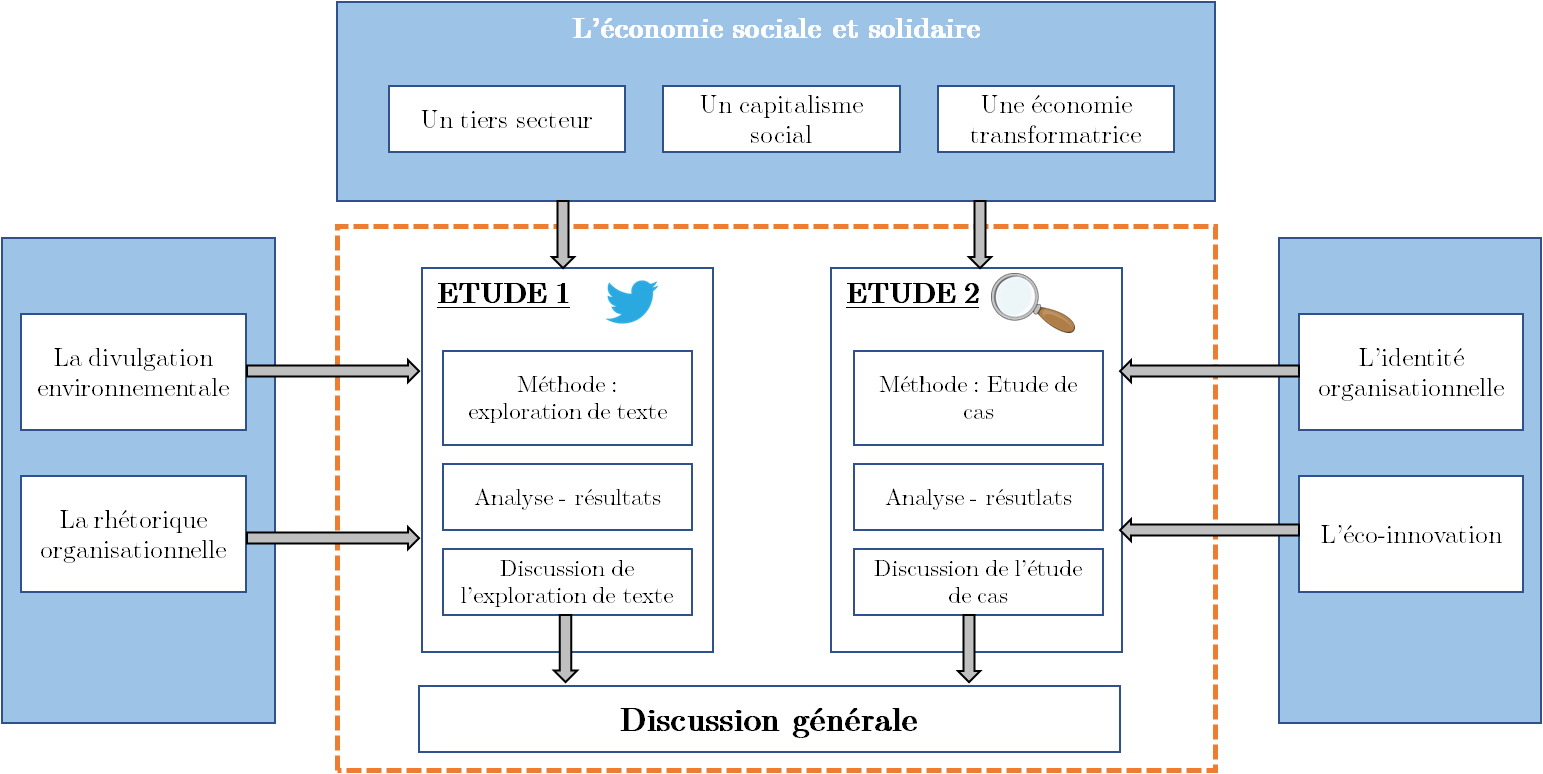
\includegraphics[width=\linewidth]{fig/methodo.png}
    \end{figure}
\end{landscape}

	La figure \ref{fig:methodoglobale} présente l'agencement général de la recherche. La première étude (chapitre \ref{chapitre:twitter}) porte sur la communication environnementale des \eess sur un réseau social destiné à tous les publics : Twitter. Nous mobilisons les méthodes de l’exploration de texte pour traiter un corpus de plus de 28 000 messages relatifs à l’environnement postés sur ce réseau. La seconde étude porte sur plusieurs cas, dans le but d'identifier, au-delà du discours, la façon dont les \eess peuvent effectivement agir pour protéger l’environnement. L’étude des cas se base sur les documents de référence des entreprises, leur site internet ainsi que sur une série d’entretiens auprès de dirigeants. \\

                \section{Communication environnementale des EESS sur Twitter}
                    
La première étude exploratoire s’intéresse au contenu diffusé par des OESS sur un des réseaux sociaux les plus utilisés dans le monde, Twitter. Elle porte donc sur le discours tenu par les organisations sur un média public. Cette recherche s’inscrit dans le champ de l’exploration de données (\textit{data mining}) et plus particulièrement de l’exploration de texte (\textit{text mining}). A ce jour, de telles méthodes sont peu mobilisées dans le champ de la recherche en management \parencite{kobayashi2018text}. Le traitement de grands volumes de données est pourtant un enjeu considérable dans un domaine dans lequel la majorité des contenus ne sont pas ou peu structurés. Cette étude combine différentes méthodes afin d’avoir une approche originale des données.

Dans un premier temps, nous présentons le réseau social Twitter et proposons une brève synthèse de l’utilisation qui en est faite dans la littérature académique. Nous expliquons ensuite de façon synthétique la démarche de collecte et d’analyse des données. Par souci de clarté, le détail de chacune des étapes de cette étude est donné dans l’annexe \ref{annexemethodo}.

\subsection{Le réseau social Twitter : utilisation et recherche}
    Depuis sa création, Twitter a suscité beaucoup d’intérêt, notamment dans le monde médiatique. Des chercheurs se sont également tournés vers ce réseau social comme objet d’étude en tant que tel, ou bien comme une source de données. L’ESS est largement représentée sur le réseau qui constitue donc une base de données mobilisable pour cette recherche. Non seulement le discours tenu sur Twitter nous informe sur l’émetteur, sur les thématiques auxquelles il accorde de l’importance et sur les stratégies qu’il adopte pour diffuser des idées, mais il peut également avoir un impact sur son audience. \textcite{gummerus2017ethical} montrent ainsi que l’implication dans une  \cit{communauté éthique} sur un réseau social en ligne entraîne une évolution du comportement de la personne impliquée – à condition qu’un management efficace de la communauté soit mis en place. \\

    Dans cette partie, nous présentons les spécificités du réseau social Twitter et montrons comment il est utilisé dans la recherche académique.


    \subsubsection{Présentation du réseau social Twitter}

        Twitter est un réseau social en ligne ayant pour mission de \citit{donner à chacun le pouvoir de créer et de partager des idées et des informations instantanément et sans entraves}\footnote{\url{https://about.twitter.com/fr/company}}. Créé en 2006, il a connu une croissance très rapide du nombre d’inscrits, jusqu’à devenir un des réseaux les plus populaires au monde. L’inscription est gratuite et ouverte à tous, particuliers et organisations. Twitter revêt un caractère généraliste et permet d’échanger sur des sujets très divers comme \citit{la musique, les sports, la politique, l'actualité, les célébrités ou tout simplement les moments du quotidien}\footnote{\url{https://support.twitter.com/articles/314982\#}}.\\

        L’utilisation de Twitter repose sur quelques fonctionnalités de base qui sont présentées ici. Cette section précise également le vocabulaire utilisé dans l’étude.

        \paragraph{Comptes d’utilisateurs.}
        L’utilisation de Twitter nécessite la création d’un compte. Celui-ci peut être public ou privé. Dans le premier cas, les messages diffusés à partir de ce compte sont visibles par tous les utilisateurs du réseau. Au contraire, les comptes privés ne sont accessibles que par des utilisateurs autorisés par le propriétaire du compte. L’usage de Twitter favorise les comptes publics : lors de la collecte des données (détaillée plus loin), seuls deux comptes privés ont été rencontrés pour 1125 comptes publics. L’utilisateur peut associer différents éléments à son compte : photo de profil, description, âge, langue, ville de résidence…
        Un compte n’est pas obligatoirement associé à une personne physique : un compte peut appartenir à une organisation ou être dédié à un évènement particulier (festival, évènement sportif…). Une personne ou une organisation peut détenir plusieurs comptes. Certains comptes sont certifiés, c’est-à-dire que le propriétaire du compte est clairement identifié. Cette fonctionnalité est généralement utilisée par les célébrités ou grandes entreprises. \\
        Par la suite, les termes de  \og comptes  \fg{} ou  \og utilisateurs  \fg{} sont employés indifféremment pour désigner les comptes d’utilisateurs.

        \paragraph{Tweets.}
        Les messages diffusés sur Twitter sont appelés des tweets. Ils sont limités à 140 caractères  et peuvent être associés à des images ou des fichiers audio ou vidéo. Il est également possible d’intégrer un lien vers une page web dans le tweet (l’URL est automatiquement raccourcie par Twitter afin de limiter le nombre de caractères utilisés). \\
        Par la suite, les termes de  \og tweets  \fg{} ou  \og messages  \fg{} sont employés indifféremment.

        \paragraph{Mentions.}
        Dans un tweet, il est possible de mentionner un autre utilisateur en écrivant son nom d’utilisateur précédé du symbole ‘@’ (par exemple ‘@CNCRES’). Celui-ci reçoit alors une notification l’informant qu’il a été mentionné. Lorsqu’un utilisateur répond à un tweet, l’émetteur du premier tweet est mentionné dans la réponse.

        \paragraph{Abonnés et abonnements.}
        Le moyen privilégié d’accéder à du contenu sur Twitter est de s’abonner à des comptes. Les tweets des comptes auxquels un utilisateur est abonné s’affichent automatiquement sur son  \og mur  \fg{}. Twitter désigne les abonnements par le terme  \og d’amis  \fg{} (friends). Inversement, les utilisateurs qui s’abonnent à un compte sont désignés par le terme de  \og followers  \fg{} (abonnés). Le nombre d’abonnés peut donc être utilisé comme un indicateur de la popularité et de l’influence sur Twitter, puisqu’il mesure l’audience d’un compte. Le lien abonné-abonnement peut être réciproque si deux utilisateurs s’abonnent l’un à l’autre. \\
        Par la suite, les termes  \og d’abonné  \fg{} et  \og abonnements  \fg{} sont utilisés.

        \paragraph{Retweets.}
        Les retweets désignent les messages publiés par un utilisateur qui sont ensuite partagés et rediffusés par d’autres utilisateurs. Un retweet est visible par les abonnés du compte qui l’a partagé, même s’ils ne sont pas abonnés à l’émetteur initial du message. Le retweet augmente donc l’audience d’un tweet et constitue un indicateur de son influence.

        \paragraph{Favoris.}
        Un utilisateur peut ajouter à ses favoris un tweet qu’il consulte. Cette fonctionnalité peut être utilisée comme un  \og marque-page  \fg{}, afin de retrouver plus tard un contenu jugé intéressant. Elle peut aussi plus simplement être utilisée pour notifier à l’auteur que l’on a apprécié le tweet, sans pour autant vouloir le partager.

        \paragraph{Hashtags.}
        Le terme de hashtag désigne les mots clés utilisés dans un tweet pour permettre son référencement. Les hashtags sont précédés du symbole \#. Ainsi, les tweets relatifs à l’ESS peuvent faire apparaitre dans le texte le hashtag ‘\#ESS’. Il est possible d’effectuer des recherches par mot clé dans l’interface Twitter : on obtiendra alors une liste de tweets intégrant le hashtag recherché. Les utilisateurs convergent souvent vers des hashtags populaires comme  \og \#socent  \fg{} pour  \og entreprise sociale  \fg{}.

        \paragraph{Type de données disponibles.}
        Un grand nombre de métadonnées sont associées à chaque compte et à chaque tweet. Certaines sont accessibles directement par l’interface web, comme le contenu du message, les mentions, les hashtags ou encore la biographie d’un utilisateur. D’autres sont privées et ne sont accessibles que par l’utilisateur lui-même ou par les administrateurs. Enfin, certaines informations sont disponibles mais ne sont pas visibles sur l’interface web. Twitter met à disposition une interface développeurs (API) permettant d’accéder à une quantité importante de métadonnées. L’ensemble des métadonnées accessibles est détaillé dans la documentation : \url{https://dev.twitter.com/overview/api}.


    \subsubsection{Twitter dans la recherche}

        Créé en 2006, Twitter constitue une source de données récente. Toutefois, le volume d’informations disponible est considérable et ce matériau a déjà été mobilisé pour la recherche. Comme le montre le tableau \ref{table:1}, des problématiques diverses peuvent être étudiées à l’aide de ce type de données, et les méthodes mobilisées sont aussi bien qualitatives que quantitatives.

        \textcite{bruns2012how} s’intéresse ainsi à la structure des conversations qui se déroulent sur le réseau et met en évidence le rôle de différents acteurs dans ces conversations. Les interactions sur le réseau intéressent aussi \textcite{xu2014talking} qui étudient la façon dont les citoyen prennent part au débat politique en relation avec les journalistes. D’autres s’intéressent à la diffusion des informations sur Twitter, en fonction des caractéristiques des images diffusées \parencite{stefanone2015image} ou de la proximité géographique, idéologique, économique ou culturelle \parencite{kwon2015spatiotemporal}. La diffusion de différentes opinions dans le cadre d’un débat (en l’occurrence celui de la neutralité du net) est également étudiée par \textcite{lee2015shaping} qui constatent un déséquilibre entre les positions exprimées. Twitter est également utilisé pour identifier des leaders d’opinion \parencite{xu2014twitter}. Les chercheurs s’intéressant à l’économie sociale ont également mobilisé Twitter comme matériau d’étude. \textcite{waters2011tweet} constatent que les organisations du secteur non lucratif adoptent une communication à sens unique, mobilisant le réseau social pour diffuser de l’information auprès de leurs abonnés. Leurs interactions avec d’autres utilisateurs sont par contre limitées et elles ne bénéficient pas de la dynamique participative rendue possible par Twitter. Deux études de \textcite{guo2014tweeting,guo2017speaking} s’intéressent à l’usage des réseaux sociaux et particulièrement de Twitter par le secteur non lucratif.  La première compare l’utilisation par ses entreprises de différents réseaux sociaux, montrant la prédominance de Facebook et Twitter. Soulignant la grande diversité d’usage de Twitter par les organisations à but non lucratif (le nombre de tweets publiés varie de 0 à plus de 1 000 dans leur panel), les auteurs montrent que ce média est utilisé principalement à titre d’information (69 \%), dans une moindre mesure àpour constituer une communauté (20 \%), et enfin pour appeler à l’action (11 \%). Onze tactiques adoptées à des fins de plaidoyers sont également mises en évidence. La seconde étude questionne la capacité à être entendu et à maintenir une audience à travers un média qui véhicule une quantité considérable d’informations dans tous les domaines. Elle montre que la taille du réseau d’un utilisateur (nombre d’abonnés), la fréquence de publications de tweets, la stratégie de ciblage (mentions d’autres comptes dans un tweet) et la diffusion de contenus visuels sont positivement associés à l’attention accordée à un tweet (mesurée par le nombre de retweets et le nombre de mises en favori). \\

        Différentes modalités de collecte et d’analyse des données sont mobilisées. \textcite{bruns2012how} a recourt au programme yourTwapper-keeper (yTK) associé au logiciel Gawk qui fonctionne en lignes de commandes. Dans plusieurs cas, le langage informatique Python est utilisé pour interroger l’API de Twitter\footnote{Grégory Saxton et son ancien doctorant Weiai Wayne Xu mettent à disposition des scripts ainsi que des tutoriels sur leurs blogs respectifs (\url{http://social-metrics.org/} et \url{http://www.curiositybits.com/}) } \parencite{guo2014tweeting,guo2017speaking,stefanone2015image,xu2014twitter,xu2014talking}. Certaines études ne précisent pas les modalités de collecte, toutefois l’usage d’un programme similaire est probable.\\

        La majorité des études s’appuient sur une combinaison de plusieurs méthodes. Les approches quantitatives sont nombreuses, mais sont dans la plupart des cas précédées d’un codage permettant de quantifier ou catégoriser les données issues de Twitter. \textcite{xu2019does} proposent toutefois une analyse quantitative sans traitement qualitatif préalable, en s'appuyant uniquement sur des données quantifiables comme le nombre d'interactions ou la centralité de l'utilisateur dans le réseau. Les statistiques descriptives sont fréquemment utilisées pour décrire le comportement des utilisateurs sur le RS et des statistiques multivariées permettent de mettre en évidence des relations entre différentes variables. Trois études ont recours à des approches visuelles des réseaux grâce à des logiciels comme Gephi ou NodeXL \parencite{bruns2012how,xu2014twitter,xu2014talking}.\\
        \clearpage

        \begin{landscape}
        \begin{spacing}{1}
        \begin{longtable}{
            |>{\setlength{\baselineskip}{0.75\baselineskip}}K{2.5cm}
            |>{\setlength{\baselineskip}{0.75\baselineskip}}K{3cm}
            |>{\setlength{\baselineskip}{0.75\baselineskip}}K{5cm}
            |>{\setlength{\baselineskip}{0.75\baselineskip}}K{6.2cm}
            |>{\setlength{\baselineskip}{0.75\baselineskip}}K{6.2cm}|}

        \caption{Utilisation de Twitter dans la recherche}
        \label{table:1} \\ \hline

            \multicolumn{1}{|c|}{\textbf{Auteurs}}
            & \multicolumn{1}{c|}{\textbf{Echantillon}}
            & \multicolumn{1}{c|}{\textbf{Focus }}
            & \multicolumn{1}{c|}{\textbf{Méthode }}
            & \multicolumn{1}{c|}{\textbf{Principaux résultats}}  \\ \hline
            \endfirsthead
            \hline
            \multicolumn{1}{|c|}{\textbf{Auteurs}}
            & \multicolumn{1}{c|}{\textbf{Echantillon}}
            & \multicolumn{1}{c|}{\textbf{Focus }}
            & \multicolumn{1}{c|}{\textbf{Méthode }}
            & \multicolumn{1}{c|}{\textbf{Principaux résultats}} \\ \hline
            \endhead
            \multicolumn{5}{|l|}{\textbf{\textit{Articles non relatifs à l’ESS ou au secteur non lucratif}}} \\ \hline

            \textcite{bruns2012how}
            &
            &Evolution des conversations twitter et rôle des acteurs
            &Collecte : yTK et Gawk \newline Analyse : visualisation des réseaux (Gephi)
            &Proposition de méthode pour une analyse dynamique
            \\ \hline

            \textcite{xu2014talking}
            &3 699 tweets retenus parmi 91015
            &Dynamiques de pouvoir entre les citoyens et les journalistes sur Twitter
            &Collecte : Python \newline Analyse qualitative (codage) permettant une analyse quantitative (statistiques descriptives)
            &Participation active des citoyens en partageant les contenus des journalistes et en exprimant leur propre opinion. Les citoyens engagés interagissent davantage avec les journalistes partageant leur orientation politique.
            \\ \hline

            \textcite{xu2014twitter}
            &125 907 tweets \newline Analyse porte sur 3 319 tweets par 2 767 utilisateurs
            &Partage des connaissances au sein d’une communauté de pratiques sur Twitter
            &Collecte : Python \newline Analyse qualitative (codage) permettant une analyse quantitative (statistiques descriptives et visualisation des réseaux)
            &Mise en évidence d’un réseau décentralisé. Les conversations ont généralement lieu entre participants ayant le même rôle et sont souvent discontinues et non-réciproques
            \\ \hline

            \textcite{xu2014predicting}
            &1 000 utilisateurs sélectionnés parmi 8 957 identifiés --> 3546 tweets
            &Identification des leaders d’opinion dans le domaine de l’activisme politique
            &Analyse des réseaux (NodeXL)\newline Analyse qualitative (codage) permettant une analyse quantitative (régressions)
            &Plus forte influence des organisations que des particuliers \newline La centralité dans le réseau impacte positivement l’influence
            \\ \hline

            \textcite{kwon2015spatiotemporal}
            &NC \newline 5 \% du volume collecté est codé
            &Diffusion des informations selon la proximité
            &Collecte : programme ad hoc. \newline Analyse qualitative (codage) permettant une analyse quantitative (modèle mathématique de la diffusion)
            &Développement d’un modèle spatio-temporel de la diffusion
            \\ \hline

            \textcite{lee2015shaping}
            &6 289 tweets \newline 150 articles analysés
            &Informations diffusées sur Twitter à propos du débat sur la neutralité d’internet
            &Analyse qualitative (codage du contenu) permettant une analyse quantitative (statistiques descriptive)
            &Diversité des parties prenantes qui s’expriment mais pas de diversité des points de vue représentés
            \\ \hline

            \textcite{stefanone2015image}
            &15 840 tweets – 290 images analysées
            &Impact des attributs de l’utilisateur et des caractéristiques images publiées sur leur diffusion sur Twitter
            &Collecte : Python ; Codage de données visuelles permettant une analyse quantitative (statistiques descriptives et multivariées, régressions)
            &Diffusion plus importante des visuels reposant sur la peur et l’humour, contrairement à la rationalité, l’émotion ou le sexe. Les messages positifs sont également mieux diffusés
            \\ \hline

            \multicolumn{5}{|l|}{\textbf{\textit{Articles relatifs à l’ESS ou au secteur non lucratif}}} \\ \hline

            \textcite{waters2011tweet}
            &27 comptes – tweets de mars 2010
            &Modalité de communication des organisations du secteur non lucratif sur Twitter
            &Analyse qualitative (codage) ; Analyse quantitative (statistiques descriptives)
            &Le réseau est principalement utilisé pour diffuser des messages à sens unique. La dimension communautaire est peu utilisée.
            \\ \hline

            \textcite{guo2014tweeting}
            &150 organisations - 750 tweets sélectionnés aléatoirement sur une période d’un mois
            &Usage des réseaux sociaux par les entreprises du secteur non-lucratif. Focus sur les tactiques de plaidoyer sur Twitter
            &Collecte :  Python ; Analyse quantitative descriptive (modalités d’usages) ; Analyse qualitative du texte, codage (identification des tactiques)
            &Utilisation principalement pour informer une audience. 11 tactiques de plaidoyer identifiées
            \\ \hline

            \textcite{guo2017speaking}
            &219 915 tweets par 145 organisations
            &Stratégie des utilisateurs pour obtenir l’attention de leur audience sur Twitter
            &Collecte :  Python ; Analyse quantitative multivariée (régressions)
            &L’attention accordée augmente avec la taille du réseau de l’émetteur, la fréquence des tweets, la stratégie de ciblage et l’adjonction de contenu visuel
            \\ \hline

            \textcite{xu2019does}
            & 198 organisations - tweets de juillet 2014 à janvier 2015
            &Lien entre les stratégies d'engagement des parties prenantes et le capital social obtenu
            &Collecte : Python; Analyse : Régressions (OLS)
            &L'obtention de capital social des \textit{nonprofits} sur Twitter dépend de la quantité, mais surtout de la qualité et de la diversité des interactions sur le réseau.
            \\ \hline

        \end{longtable}
        \end{spacing}
        \end{landscape}



    Encore peu utilisés comme source de données pour la recherche académique, les réseaux sociaux \citit{offrent nombre de challenges et d'opportunités pour les chercheurs qui s'intéressent au reporting et à la responsabilité des entreprises} \parencite[][p. 161]{saxton2016csr}. Plusieurs raisons nous ont poussé à choisir Twitter pour notre recherche. Tout d'abord, d'un point de vue pratique, le réseau offre un accès facile aux données,  à l'aide d'une API (interface technique permettant de communiquer avec la base de données de tweets). Dans la mesure où les tweets sont très majoritairement publics (seule une minorité d'utilisateurs choisissent de limiter l'accès à leurs publications), les données peuvent être collectées avec peu de restriction. A l'inverse, l'accès aux données des réseaux sociaux comme Facebook ou Linkedin est beaucoup plus limité et contrôlé. Le deuxième aspect pris en compte est celui du volume de données. L'obtention de suffisamment de données est souvent un enjeu en sciences de gestion. Or, quel que soit le champ étudié, le volume de données produit chaque jour sur Twitter est considérable. Des entreprises de tous les secteurs d'activités disposent d'un compte, mais aussi des politiciens, journalistes ou simplement des personnes intéressés par une grande variété de sujets. Si la qualité des données peut soulever des difficultés et nécessité des traitements préalables, elles sont en revanche en quantité illimitée et sans cesse renouvelées. Sur le fond, le contenu apporte une richesse supplémentaire par rapport à des documents institutionnels, en ceci qu'il dépasse le simple reporting pour établir une réelle communication \parencite{saxton2016csr}. Pour Saxton, les entreprises présentes sur Twitter ne peuvent se limiter à une communication unidirectionnelle, mais sont amenées à interagir avec leurs parties prenantes, qui peuvent les interpeler. Twitter est donc \citit{un outil d'éducation public et de mobilisation} \parencite[][p. 164]{saxton2016csr}. Il est tout à fait pertinent pour étudier les questions qui se rapportent à la RSE, celles-ci étant étroitement liées à l'interaction entre les entreprises et leurs parties prenantes. Nous nous appuyons sur cette littérature pour mettre en place notre étude du discours des \eess sur Twitter. Quelques recherches se sont déjà intéressées aux pratiques du secteur non lucratif sur le réseau social \parencite{waters2011tweet, guo2014tweeting, guo2017speaking}. Cependant, à notre connaissance, notre étude est la première à élargir le spectre au périmètre plus étendu de l'ESS et à comparer le discours tenu par les organisations ayant différents statuts. \\


    Dans les sections suivantes, nous présentons le processus de collecte des données, puis les différentes étapes de l'analyse. Celles-ci sont résumés dans le tableau \ref{table:etapestwitter}.

                    \begin{table}
	\caption{Etapes de l'étude}
    \label{table:etapestwitter}
    \begin{tabularx}{\linewidth}{
        |K{0.10\linewidth}
        |K{0.20\linewidth}
        |L
        |L
        |}
    	\hline
    	\textbf{Section} & \textbf{Etape} & \textbf{Analyses réalisées} & \textbf{Objectifs} \\ \hline

        \ref{twitter:collecte}
        & \multicolumn{3}{|l|}{\textbf{\textit{1 - Collecte des données}}} \\ \hline

        \ref{twitter:analysegenerale}
        & \multicolumn{3}{|l|}{\textbf{\textit{2 - Approche générale du corpus}}} \\ \hline

            \ref{twitter:commu}
            & Etude des communautés
            & Analyse des réseaux
            & Identifier les communautés d'OESS sur le réseau social
            \\ \hline

            \ref{twitter:attention}
            & Statistiques multivariées
            & Régressions linéaires multiples
            & Etudier le niveau d'attention obtenu par les tweets dans le contexte de l'ESS en France
            \\ \hline

            \ref{twitter:placediscours}
            & Place du discours environnemental
            & Tests statistique de comparaison de moyennes
            & Déterminer la place de l'environnement dans le discours des différents types d'organisations
            \\ \hline


        \ref{twitter:exploration}
        & \multicolumn{3}{|l|}{\textbf{\textit{3 - Exploration de texte}}} \\ \hline

            \ref{twitter:thematiques}
            & Extraction des thématiques principales
            & Classification automatique non supervisée
            & Identifier les principales thématiques environnementales traitées par les utilisateurs
            \\ \hline

            \ref{twitter:strategies}
            & Etude des stratégies rhétoriques
            &  Classification automatique  supervisée ;\newline Classification analytique ;\newline Analyses factorielles des correspondances
            & Comparer les stratégies rhétoriques des différents types d'organisations
            \\ \hline

            \ref{twitter:perf}
            & Performance des tweets selon la stratégie
            & Tests statistiques paramétriques et non paramétriques
            & Déterminer si la stratégie rhétorique impacte le niveau d'attention obtenue par les tweets
            \\ \hline

    \end{tabularx}
\end{table}



\subsection{Collecte des données}
    \label{twitter:collecte}
    La collecte des données est faite en deux étapes. La première vise à la constitution d’une liste d’utilisateurs appartenant au champ de l’ESS et la seconde télécharge les tweets de ces utilisateurs (avec les méta-données associées). Pour interroger la base de données de Twitter (API) et extraire ces informations, nous avons écrit des scripts dans le langage informatique Python\footnote{Les scripts ont été regroupés dans un programme disponible en accès public: \url{https://github.com/newbisebi/twitSearch}}. \\

    L’échantillon est constitué de comptes Twitter d’OESS. Une première liste a été constituée à partir de sources externes (CNCRES, ACP, data.gouv). Des organisations référencées dans ces sources et disposant d’un compte Twitter ont été intégrées au panel. La liste est ensuite complétée par une recherche interne par mots-clés dans l’interface Twitter, ainsi qu’en utilisant la fonctionnalité « suggestions » proposée par le réseau social. Les critères d’intégration ou de non intégration des comptes à l’échantillon sont détaillés en annexe. Nous avons collecté les informations associées à chaque utilisateur et avons déterminé manuellement pour chacun le type d’organisation et le caractère environnemental (Tableau \ref{table:donneesutilisateurs}). Sept types d’organisations sont retenus : mutuelle, coopérative, association, fondation, entreprise sociale, fédération et organismes de représentation (structures visant à rassembler d’autres OESS ou qui ont un rôle de représentation) et la catégorie autre, qui rassemble les incubateurs dédiés à l’ESS et les comptes Twitter correspondant à des marques ou des évènements en lien avec l’ESS. Le caractère environnemental indique si la mission principale est liée à la préservation de l’environnement. \\


    \begin{table}[h]
        \caption{Données relatives aux comptes d'utilisateurs}
        \label{table:donneesutilisateurs}
        \begin{tabularx}{\linewidth}{|l|X|}
            \hline
            \textbf{Nom} & \textbf{Description} \\ \hline
        \multicolumn{2}{|l|}{\textbf{\textit{Données collectées sur Twitter}}} \\ \hline
            Nom utilisateur &	Nom d’identification de l’utilisateur (différent du nom affiché) \\ \hline
            Id utilisateur &	Numéro unique d’identification de l’utilisateur  \\ \hline
            Description	 & Biographie de l’utilisateur sur son profil \\ \hline
            Nombre d’abonnements &	Nombre de comptes auxquels l’utilisateur est abonné (‘friends’) \\ \hline
            Nombre d’abonnés &	Nombre de comptes abonnés à l’utilisateur (‘followers’) \\ \hline
            Nombre de tweets &	Nombre de tweets publiés par l’utilisateur (hors tweets supprimés) \\ \hline
        \multicolumn{2}{|l|}{\textbf{\textit{Données ajoutées a posteriori}}} \\ \hline
            Catégorie du compte	& Catégorisation de l’utilisateur en fonction du statut ou de la forme de l’organisation  \\ \hline
            Organisation environnementale	& Variable booléenne : ‘vrai’ si la mission principale de l’entreprise est directement liée à la préservation de l’environnement  \\ \hline
        \end{tabularx}
    \end{table}

    Pour chacun des utilisateurs, nous avons extrait les tweets postés avant le 30 juin 2017 (les plus anciens tweets datent de 2008). Les critères d’extractions ne retiennent que les tweets originaux (c'est-à-dire que les tweets republiés ou retweets sont exclus) et en français (cette indication peut toutefois être incorrecte et certains tweets en anglais ont été collectés). Les méta-données extraites sont présentées dans le Tableau \ref{table:donneestweets}.


    \begin{table}[h]
        \caption{Données relatives aux tweets}
        \label{table:donneestweets}
            \begin{tabularx}{\linewidth}{|l|L|}
                \hline
                \textbf{Nom} & \textbf{Description} \\ \hline
                Id tweet&	Numéro unique d’identification du tweet \\ \hline
                Nom utilisateur&	Nom de l’utilisateur ayant posté le tweet \\ \hline
                Id utilisateur&	Identifiant de l’utilisateur ayant posté le tweet \\ \hline
                Date&	Date exacte de publication du tweet au format AAAA-MM-JJ hh:mm:ss.000000 \\ \hline
                Année&	Année de publication du tweet (format AAAA) \\ \hline
                Mois&	Mois de publication du tweet (format MM) \\ \hline
                Texte&	Texte complet du tweet \\ \hline
                Hashtags&	Mots clés utilisés dans le message (précédés de ‘\#’) \\ \hline
                Nombre favoris*	&Nombre de fois où le tweet a été mis en favori \\ \hline
                Nombre retweets*&	Nombre de fois où le tweet a été partagé \\ \hline
                Id mentions	&Identifiant numérique des utilisateurs mentionnés dans le tweet \\ \hline
                Nom mentions&	Nom des utilisateurs mentionnés dans le tweet \\ \hline
                 \multicolumn{2}{K{0.95\linewidth}}{\footnotesize{*Ces données sont susceptibles d’évoluer dans le temps. Elles ne sont donc pas représentatives pour les tweets récents et ont onc été mise à jour un mois après la fin de la collecte pour garantir une certaine fiabilité.}}
            \end{tabularx}
    \end{table}

    Pour chaque tweet, un algorithme détermine s’il concerne des thématiques en lien avec l’environnement. Il vérifie si le tweet comporte un mot ayant la racine ‘environn’ ou ‘écolo’, ou s’il contient un mot clé (‘hashtag’) relatif à l’environnement. Pour cela, nous avons extraits les 3 000 hashtags les plus fréquents dans les tweets ; ceux identifiés comme liés à l’environnement ont été intégrés à l’algorithme.

    L’étude se focalise sur les tweets ayant un caractère environnemental. Cette sélection conduit à réduire considérablement le nombre de tweets étudiés. En effet, parmi l’ensemble des contenus publiés par les utilisateurs de l’ESS, seule une faible proportion concerne l’environnement. Ceci s’explique d’une part par le fait que seule une minorité d’\eess a une mission environnementale, et d’autre part parce que toutes sont confrontées à des sujets très variés. L’environnement ne constitue donc qu’une partie de leur discours. Cette apparente perte d’information n’est pas dommageable et correspond aux pratiques observées dans la littérature. En effet, la nature de la source de données (Twitter) fait qu’il est plus simple de collecter un ensemble de données très large et de le réduire ensuite. Ainsi, pour des études similaires, \textcite{kwon2015spatiotemporal} ne codent que 5 \% des données collectées, \textcite{stefanone2015image} analysent 290 images collectées parmi 15 840 tweets et \textcite{xu2014twitter} limitent leur analyse à 3 319 tweets sur 125 907 collectés.

\subsection{Analyse générale du corpus}
    \label{twitter:analysegenerale}
    Une première phase de l'étude s'intéresse au corpus dans son ensemble. Elle porte donc sur la totalité des comptes d'utilisateurs et des tweets collectés, avant la suppression des tweets ne parlant pas d'environnement. Dans un premier temps, une visualisation des communautés d'utilisateurs est proposée. Dans un second temps, nous menons une approche statistique du niveau d'attention obtenus par les tweets. Finalement, nous nous intéressons à la place du discours environnemental dans le corpus.

    \subsubsection{Etude des communautés}
        \label{twitter:commu}
        La fonction première des réseaux sociaux est de lier entre eux les utilisateurs. L’étude des réseaux s’intéressent donc aux relations et aux interactions entre les utilisateurs de ces réseaux. A partir des relations d’abonnement (un utilisateur s’abonne aux tweets d’un autre) réciproques ou non et des interactions directes (mention d’un autre utilisateur dans un tweet), nous identifions les communautés qui se créent. Le logiciel Gephi permet de visualiser ces communautés et les interactions entre elles. On cherche ici à découvrir comment les acteurs de l’ESS s’organisent et interagissent sur le réseau social Twitter.

    \subsubsection{Niveau d'attention}
        \label{twitter:attention}

        \textcite{guo2017speaking} ont recours à des statistiques multivariées pour prédire l’audience d’un tweet d’une organisation du secteur non lucratif sur Twitter en fonction de son utilisation du réseau. En particulier, les auteurs obtiennent les résultats suivants : \\
        R1 – Le niveau d’attention reçu par un compte est associé positivement au nombre d’abonnés. \\
        R2 – Le niveau d’attention reçu est associé positivement avec le nombre de tweets publiés. \\
        R3 – Le nombre de retweets est associé négativement avec le nombre de réponses à d’autres utilisateurs, mais le nombre de favoris est associé positivement avec le nombre de réponses. \\
        R4 – Le niveau d’attention reçu par un compte est associé positivement avec le nombre de hashtags utilisés.\\
        R5 – le niveau d’attention n’est pas significativement lié au nombre de tweets mentionnant d’autres utilisateurs.\\

        Nous menons une étude similaire afin de tester si les mêmes résultats sont obtenus dans un contexte national différent (la France VS les États-Unis) et avec un périmètre plus large (l’ESS VS le secteur non lucratif). Notre design est inspiré de celui de Guo et Saxton, mais n'est pas reproduit à l'identique. Contrairement aux auteurs, nous ne prenons pas en compte la temporalité : les données sont une agrégation de l’ensemble de la période. Nous faisons ceci afin de garantir l'indépendance des modalités de la variable expliquée (chacune correspond à un compte différent) \parencite{field2009discovering}. En outre, pour tenir compte de la variété des \eess étudiées, nous nous appuyons sur un échantillon substantiellement plus important (910 649 tweets VS 219 915).
        Le Tableau \ref{table:10comparaisonguo} compare les modalités de l’étude avec celles de Guo et Saxton. Deux régressions sont effectuées, avec en variable expliquée le nombre de retweets, puis le nombre de favoris.

        \begin{table}
        \caption{Comparaison du design avec Guo et Saxton (2017)}
        \label{table:10comparaisonguo}
            \begin{tabularx}{\linewidth}{|>{\bfseries}p{3cm}|X|X|}
             \hline
             & \textbf{\textcite{guo2017speaking}} & \textbf{Présente étude} \\ \hline
             Périmètre	& Secteur non lucratif (nonprofits) &	ESS \\ \hline

            Unité \newline d’analyse	& Compte Twitter pour un mois donné (chaque compte est représenté 12 fois)	& Compte Twitter sur la globalité de la période \\ \hline

            Effectif&	219 915 tweets - 145 organisations (N=1679*)	& 910 649 tweets - 1 100 organisations (N=1 100) \\ \hline

            \multirow{2}{=}{Variables expliquées	}
                &Nombre de retweets & Nombre total de retweets  \\
                &Nombre de favoris & Nombre total de favoris \\ \hline

            \multirow{10}{=}{Variables explicatives}
                &Nombre de tweets & Nombre de tweets \\
                &Nombre de réponses & Nombre de réponses \\
                &Nombre d’abonnés & Nombre d’abonnés \\
                &Nombre de hashtags dans le tweet & Nombre de tweets avec au moins un hashtag \\
                &Nombre de tweets avec au moins une mention & Nombre de tweets avec au moins une mention \\
                &Nombre de retweets d’autres utilisateurs & Nombre d’abonnements  \\
                &Nombre de tweets avec photos &  \\
                &Nombre de tweets avec lien vers une photo &  \\
                &Nombre de tweets avec lien vers une vidéo & \\
                &Nombre de tweets avec au moins une URL & \\ \hline

            \multirow{2}{=}{Variables de contrôle	}
                &Taille de l’organisation & Type d’entreprise \\
                &Age de l’organisation&\\ \hline

            \multirow{2}{=}{Type de régression	}
                &Moindres carrés ordinaires & Moindres carrés ordinaires\\
                &Effets fixes&\\ \hline

            \end{tabularx}
            \footnotesize
                * \textit{145 entreprises sur 12 mois devrait donner N = 1 740, mais certaines n'ont pas twitté pendant certains mois. Ici, notre design diffère en ceci qu'on ne prend pas en compte la temporalité : chaque entreprise correspond à un individu unique dans la régression. }
        \end{table}

    \subsubsection{Place du discours environnemental}
    \label{twitter:placediscours}
        Pour terminer cette approche générique du corpus, une comparaison des différentes catégories d'entreprises est menée à l'aide de tests statistiques. D'une part, nous comparons le pourcentage moyen de tweets relatifs à l'environnement entre les organisations dont l'activité est liée à l'écologie et celles dont l'activité est autre. D'autre part, nous comparons le pourcentage moyen de tweets relatifs à l'environnement entre les différentes catégories d'organisations. La variable étudiée est la moyenne du pourcentage de tweets environnementaux calculé pour chaque organisation. Par conséquent, ce taux est impacté par la proportion d'entreprises à caractère environnemental dans l'échantillon. Pour neutraliser cet impact, les tests de comparaison sont reproduits après élimination des entreprises environnementales. Ceci permet de mesurer la place de l'environnement dans la communication des organisations dont la mission n'est pas à caractère environnemental. En effet, comme l'a montré la revue de la littérature, les motivations à communiquer sur ces enjeux sont multiples. Si les entreprises à mission environnementale ont des raisons évidentes de communiquer sur ces thématiques, les autres organisations ont également des motivations à s'emparer du sujet.

        Des tests non paramétriques sont utilisés pour tenir compte de la non-normalité des distributions.

\subsection{L'exploration de texte}
\label{twitter:exploration}
    Une définition courante de l’exploration de texte est celle de \textcite[][p. 1]{kao2010natural} \citit{la découverte et l’extraction de connaissances intéressantes et non triviales à partir de textes non structurés}. Comme nous l’avons vu dans la partie précédente, les données issues de Twitter sont assez structurées et s’accompagnent de nombreuses données quantitatives. Toutefois, l’apport de l’exploration de texte est évident pour l’étude du contenu même des tweets. Elle permet de donner du sens aux textes lorsque le volume est trop important pour permettre un codage ou même une lecture flottante \parencite{kobayashi2018text}. Cette étude se limite au contenu en lien avec les problématiques environnementales. Seuls les tweets identifiés comme ayant trait à l'écologie sont conservés. Cette phase est menée en trois temps. En premier lieu, l'usage d'algorithmes de classification non supervisée permet de faire émerger les principales thématiques abordées dans le corpus. En second lieu, deux classifications supervisées et analytiques permettent de distinguer plusieurs stratégies rhétoriques. Enfin, nous mesurons la performance obtenue par les tweets en fonction des stratégies de communication.


    \subsubsection{Extraction des thématiques principales}
    \label{twitter:thematiques}
        L’extraction de thématiques s’appuie sur des modèles probabilistes qui permettent de générer automatiquement des catégories à partir des mots du texte (Kobayashi et al., 2018). Selon ces auteurs, la méthode LDA (latent Dirichlet allocation) est la plus communément utilisée. Nous comparons les résultats de cet algorithme avec ceux du modèle NMF (Non-Negative Matrix Factorization). Ces deux procédés sont mis en œuvre sous Python.
        Ces méthodes sont non supervisées, c'est-à-dire qu’elles ne nécessitent pas de phase d’apprentissage. Toutefois, elles nécessitent la détermination a priori du nombre de thématiques à extraire. Nous avons donc procédé par itération avec différentes valeurs jusqu’à obtenir des catégories ayant du sens.

        % \todo[inline]{\textcite{ross2013common} =>  étudient les topics }

    \subsubsection{Étude des stratégies rhétoriques}
    \label{twitter:strategies}
        \paragraph{Étude du sentiment et de l'objectivité} \ \\
            A l’inverse de l’extraction de thématiques, la classification automatique est une méthode supervisée qui nécessite une phase d’entraînement du programme. Le chercheur doit fournir à l’algorithme des données pré-codées, afin \cit{d'apprendre} à la machine à reproduire ce codage. Une application courante de cette méthode est l’analyse des sentiments qui permet de déterminer si un contenu à une tonalité positive ou négative. 430 tweets extraits aléatoirement ont été codés manuellement selon deux critères : le sentiment \parencite{solomon2011private} et l’objectivité \parencite{waldron2016how}. Le premier critère détermine si la question environnementale est abordée à travers les causes, les risques et les conséquences (sentiment négatif) ou bien sous l’angle des alternatives et des opportunités qui en découlent (sentiment positif). L’objectivité traite de la façon dont le tweet est \cit{cadré} (framed) et indique si le contenu se veut factuel, appuyé sur des chiffres, des études, ou s’il transmet plutôt une opinion ou un objet de débat (Nisbet, 2009). Cette approche est similaire à celle utilisée par \textcite{cho2010language}, qui utilisent un logiciel, \textit{DICTION} pour étudier l'optimisme et la conviction dans les rapports \rse des entreprises.
            Le modèle est appliqué à l’aide de l’algorithme Naives-Bayes implémenté en Python. Suite à la phase d’apprentissage, le programme attribue à chaque tweet une valeur positive ou négative et objective ou subjective.
            Ceci permet de déterminer d’une part les stratégies rhétoriques les plus employées et par qui, et d’évaluer celles qui conduisent au meilleur niveau d’attention d’un tweet (mesuré par le nombre de retweets et le nombre de favoris). La comparaison de la performance des stratégies est faite à l’aide de tests statistiques de comparaisons de moyennes. \\

            Cette analyse est complétée par une AFC qui vise à mettre en relation les utilisateurs d’une part, et les catégories de discours employées d’autre part. Pour cela, une table de contingence est constituée sous Python. Elle indique pour chaque utilisateur (en lignes) le nombre de tweets correspondants aux quatre catégories de discours (en colonnes) : objectif, subjectif, positif, négatif. L’analyse factorielle est menée sous R à partir de cette table de contingence et aboutit à la production d’une carte factorielle. L’analyse s’intéressera particulièrement aux valeurs les plus significatives, c'est-à-dire aux utilisateurs fortement caractérisés par une des stratégies rhétoriques.

    \paragraph{Étude du cadrage du discours} \ \\

        La classification menée à cette étape vise à comprendre plus précisément le sens des messages diffusés sur le réseau. L’analyse lexicale permet d’étudier isolément les mots du corpus, c'est-à-dire détachés de leur contexte. Elle repose sur la quantification des formes lexicales. L’étude s’appuie spécifiquement sur les hashtags, c'est-à-dire les éléments du tweet mis en avant par l’émetteur du message (47.3 \% du total des tweets collectés contiennent des hashtags). L’étude utilise les hashtags pour déterminer le cadre rhétorique dans lequel s’inscrit un message. Les cadres renvoient à la façon dont le discours donne du sens à son objet. Comme le souligne \textcite{nisbet2009communicating}, toute information s’inscrit dans un cadre donné. L'auteur identifie huit cadres utilisés dans la communication sur le changement climatique, qui peuvent s’appliquer à l’ensemble des enjeux écologiques. Le  tableau \ref{table:6} présente ces cadres et précise les modalités d’opérationnalisation.



        \begin{landscape}
            \begin{spacing}{1}
            \begin{small}
            \begin{longtable}{
            |K{0.18\linewidth}
            |K{0.38\linewidth}
            |K{0.40\linewidth}
            |}
            \caption{Typologie des cadres du discours}
            \label{table:6} \\
                \hline
                \textbf{Cadre} & \textbf{Définition \parencite{nisbet2009communicating} \newline Frames define science-related issue as…} & \textbf{Opérationnalisation}\\ \hline
                \endfirsthead
                \hline
                \textbf{Cadre} & \textbf{Définition \parencite{nisbet2009communicating}} & \textbf{Opérationnalisation}\\ \hline
                \endhead
                \hline
            Progrès Social
            &A means of improving quality of life or solving problems; alternative interpretation as a way to be in harmony with nature instead of mastering it.
            &Le cadre est élargi aux hashtags qui renvoient à des questions d’ordre sociétal
            \\ \hline

            Développement économique et compétitivité
            &An economic investment; market benefit or risk; or a point of local, national, or global competitiveness.
            &Le cadre intègre tous les hashtags qui renvoient à des dimensions d’économie, d’emploi, de compétitivité ou à la notion de marché
            \\ \hline

            Moralité et éthique
            &A matter of right or wrong; or of respect or disrespect for limits, thresholds, or boundaries.
            &Le cadre intègre tous les hashtags renvoyant à la morale, à des valeurs sociales, de respect ou de solidarité.
            \\ \hline

            Incertitude scientifique et technique
            &A matter of expert understanding or consensus; a debate over what is known versus unknown; or peer-reviewed, confirmed knowledge versus hype or alarmism.
            &Hashtags renvoyant plus généralement à de questions techniques et scientifiques, sans prise de position explicite
            \\ \hline

            Boîte de Pandore, Monstre de Frankenstein et ‘Sauve-qui-peut’
            &A need for precaution or action in face of possible catastrophe and out-of-control consequences; or alternatively as fatalism, where there is no way to avoid the consequences or chosen path.
            &Hashtags renvoyant à une dimension dramatique, focalisée sur les dangers et les risques liés à la non prise en compte de l’environnement, ainsi que les conséquences déjà observées
            \\ \hline

            Responsabilité publique et gouvernance
            &Research or policy either in the public interest or serving special interests, emphasizing issues of control, transparency, participation, responsiveness, or ownership; or debate over proper use of science and expertise in decisionmaking (“politicization”).
            &Hashtags renvoyant à la gouvernance aussi bien au niveau des entreprises que des institutions publiques, ainsi que les hashtags renvoyant à une responsabilité partagée, citoyenne
            \\ \hline

            Alternatives et compromis
            &A third way between conflicting or polarized views or options.
            &Hashtags renvoyant à des alternatives, des exemples d’innovations, ou plus généralement un changement, une transition
            \\ \hline

            Conflits et stratégies
            &A game among elites, such as who is winning or losing the debate; or a battle of personalities or groups (usually a journalist-driven interpretation).
            &Hashtags renvoyant à des acteurs du débat public, à des lieux d’échange et de constitution de stratégies, ou à des prises de position claires
            \\ \hline


            \end{longtable}
            \end{small}
            \end{spacing}
        \end{landscape}

        A l'inverse des classifications précédentes, la classification n'est pas réalisée par des algorithmes, mais par une règle d'affectation mise en place par le chercheur. Elle permet donc une lecture plus fine du corpus, permettant d'apporter des résultats plus précis, mais implique une part plus grande de subjectivité.

        Comme précédemment, cette classification donne lieu à une analyse factorielle des correspondances (AFC) qui permet de confronter les différents modèles d’entreprises de l’ESS avec les cadres utilisés.

    \subsubsection{Etude de la performance des tweets }
        \label{twitter:perf}

        La performance d'un tweet, c'est-à-dire le niveau d'attention obtenu par le tweet, est généralement mesurée par deux indicateurs : le nombre de retweets et le nombre de favoris \parencite{guo2017speaking}. Nous utilisons ces deux indicateurs pour comparer la performance des tweets en fonction de la rhétorique (sentiment, objectivité, catégories de discours). A nouveau, des tests paramétriques (test T) et non paramétriques sont effectués.

        Un biais possible des deux indicateurs utilisé est que le nombre de retweets et de favoris est fortement influencé par le nombre d'abonnés d'un compte. Ceci risque de réduire la validité des résultats. Pour éliminer cet effet, nous utilisons un indicateur composite qui s'appuie à la fois sur le nombre de retweets et le nombre de favoris, mais rapportés au nombre d'abonnés. Il est calculé selon la formule suivante : \\

            \begin{center}
                $Engagement = \dfrac{Nombre\ de\ retweets + Nombre\ de \ favoris}{Nombre\ d'abonnés} \times 1 000$ \\
            \end{center}

        Le facteur 1 000 utilisé dans le calcul n'a pas d'impact sur l'analyse, celle-ci visant à comparer le ratio entre les entreprises. Il est ajouté, de manière arbitraire, à des fins de lisibilité et pour corriger l'écart d'ordre de grandeur entre le nombre de retweets et de favoris et le nombre d'abonnés. Dans l'échantillon étudié, le nombre moyen de retweets est de 3,36 et celui de favoris de 3,18, alors que les utilisateurs ont en moyenne 6 448,18 abonnés (soit environ 2 000 fois plus).


Cette recherche explore en profondeur un corpus de données important, en mobilisant des méthodes automatiques ou semi-automatiques. Ces méthodes sont adaptées à un grand volume de données et permettent de faire émerger des tendances. Cependant, la principale limite est qu'elle implique une forte distance par rapport au contenu et ne permet pas une compréhension fine du discours. En outre, cette étude porte sur le discours, la communication des organisations. Dans la partie suivante, nous présentons une seconde recherche qui vient compléter la première à l'aide d'une approche qualitative.

                \section{Leviers de l'action environnementale : étude de cas}
                    Le premier volet de la thèse concerne l'étude du discours environnemental des \eess. Celle-ci est importante car la communication permet d'adresser les demandes des parties prenantes. En outre, elle semble causer un effet d'entraînement sur les actions concrètes de protection de l'environnement \parencite{frandsen2011rhetoric}. Ce sont ces actions environnementales qui sont l'objet de notre second volet. A travers l'étude qualitative de sept cas d'entreprises, nous cherchons à identifier les leviers d'action environnementale dans l'ESS, ainsi que les facteurs qui motivent ou font obstacle à cette action. Nous nous appuyons pour cela sur des entretiens semi-directifs complétés par des documents (cf. tableau \ref{table:casetudies}). \\

Les cas étudiés ont été sélectionnés parmi des organisations installées dans la région Provence-Alpes-Côte d'Azur, et reconnus par l'INSEE comme appartenant au champ de l'ESS tel que défini par la loi de 2014\footnote{Nous nous sommes appuyé pour cela sur la base de données SIREN mise à disposition par l'INSEE, et qui comporte un champ indiquant cette appartenance}. Les entreprises susceptibles d'avoir une action environnementale (même réduite) ont été privilégiées. En effet, l'étude d'un cas d'organisation sans aucune action environnementale, quoiqu'elle puisse nous renseigner sur les barrières rencontrées, apporte peu d'éléments sur les déterminants. Cependant, l'étude ne se limite pas à des organisations directement concernées par l'action environnementale : nous cherchons à déterminer si l'appartenance à l'économie sociale favorise ou non l'action environnementale, y compris pour des organisations ayant une mission distincte. Ainsi, deux organisations du panel ont une mission environnementale (la Tour du Valat agit pour la protection des zones humides, et Air PACA opère dans le secteur de la qualité de l'air). Trois entreprises ont un lien indirect avec l'environnement : Provence Forêt, coopérative forestière ; AMS Environnement, qui a une activité d'entretien des espaces verts et Bzzz qui produit du miel et produit dérivés du miel. Finalement, Arborescence (groupe d'insertion par le travail) et Enfants et Loisirs (crèche), n'ont pas une activité environnementale a priori. L'échantillon cherche également à refléter la variété des structures organisationnelles de l'ESS. Il se compose ainsi d'une fondation, de quatre associations (dont une structure d'insertion) et de deux coopératives (dont une SCIC). Enfin, nous avons également privilégié des organisations nous donnant accès à des documents internes et dont les dirigeantes ou dirigeants ont pu se rendre disponibles pour réaliser des entretiens. 


\begin{longtable}{
        |>{\setlength{\baselineskip}{0.75\baselineskip}}K{0.18\linewidth}
        |>{\setlength{\baselineskip}{0.75\baselineskip}}K{0.16\linewidth}
        |>{\setlength{\baselineskip}{0.75\baselineskip}}K{0.18\linewidth}
        |>{\setlength{\baselineskip}{0.75\baselineskip}}K{0.48\linewidth}
    |}

        \caption{Cas étudiés}
        \label{table:casetudies} \\
        \hline
        \textbf{Organisation} & \textbf{Type} & \textbf{Entretien} & \textbf{Documents} \\ \hline
        \endfirsthead

        \hline
        \textbf{Organisation} & \textbf{Type} & \textbf{Entretien} & \textbf{Documents} \\ \hline
        \endhead

        Tour du Valat	& Fondation	& Directeur Général
        & - Plan stratégique \newline - Brochure \newline - Rapports annuels
        \\ \hline

        AMS Environnement &	Association	&Directeur
        & - Vidéo sur l'insertion
        \\ \hline

        Enfants et Loisirs &	Association	& Directrice
        &	- Projet social \newline - Projet éducatif et pédagogique \newline - Statuts \newline - Site web - écolocrèche
        \\ \hline

        Arborescence &	Coopérative	& Président
        & - Plaquette
        \\ \hline

        Provence Forêt	& Coopérative 	& Responsable environnement
        & - Plaquette \newline - Statuts \newline - Politique de gestion durable \newline - Engagement des propriétaires forestiers \newline - Newsletters (2015 et 2016)
        \\ \hline

        Air PACA	& Association	& Directeur
        & - Bilan 2016
        \\ \hline

        Bzzz	& Association	& Co-président
        & - CR conseil collégial (4) \newline - newsletters (3) \newline - PV AG 2017 \newline - Rapports d'activité 2016 et 2017 \newline - Rapport financier 2017 \newline - Statuts \newline -Programme prévisionnel 2018 \newline - Site web (Actions militantes - la Bzzz Mobile - Méthodes apicoles - valeurs et partenariats) \newline - 2 vidéos de présentation \newline - Formulaire de candidature au financement "mon projet pour la planète"
        \\ \hline

\end{longtable}

    \textcite[][p. 29]{yin2009case} décrit l'étude de cas comme \citit{une voie méthodologique rigoureuse} s'appuyant sur des \citit{procédures formelles et explicites}. L'auteur écarte ainsi d'emblée la vision d'une méthode purement interprétative, qui ne pourrait être utilisée qu'à titre d'exemple. Au contraire, Yin affirme que l'étude de cas peut être utilisée aussi bien à des fins d'exploration que de validation. Dans les deux cas, chaque étape doit être rigoureusement menée et documentée afin d'éviter les biais de validation. Yin décrit donc les modalités de l'étude de cas réaliste, c'est à dire qui admet l'existence \citit{d'une réalité unique indépendante de l'observateur} (p. 42).
    L'étude de cas est particulièrement pertinente lorsque l'on souhaite étudier un phénomène de manière détaillée et dans le cadre du contexte réel dans lequel il se produit. Elle permet aussi d'approfondir la compréhension lorsque \citit{les frontières entre le phénomène et le contexte ne sont pas clairement évidentes} \parencite[][p. 41]{yin2009case}. \\

    Pour garantir la validité de l'étude, nous nous appuyons sur un guide d'entretien élaboré à partir de la littérature. Il permet de maintenir une consistance entre les différents entretiens et de permettre une comparaison fiable. Le contenu des entretiens est retranscrit et codé à l'aide du logiciel Nvivo. Dans cette section, nous précisons la démarche d'élaboration du guide d'entretien et le processus de codage, et expliquons comment le concept d'identité organisationnelle est adapté à l'analyse.


\subsection{Élaboration du guide d’entretien}

    Le recours à l'entretien semi-directif nécessite le recours à un guide d'entretien (annexe \ref{annexe:guide}). Celui-ci s'appuie sur des questions ouvertes dont la vocation n'est pas d'être traitées successivement, mais d'établir la liste des thématiques à aborder avec les répondants. \\

    Le guide d'entretien est constitué à partir de la littérature et est guidé par la problématique.

    Une première partie de l'entretien porte sur des questions générales de compréhension des mécanismes de l'entreprise. Elles s'appuient sur les dimensions organisationnelles identifiées dans la littérature, à savoir la dimension utilitariste, la dimension normative, la dimension collective et la dimension fonctionnelle. Concernant la dimension utilitariste, il est demandé au répondant de présenter le modèle économique de l'organisation pour comprendre la place de la dimension commerciale dans son fonctionnement. Les personnes interrogées s'expriment également sur les valeurs et la finalité de l'organisation, afin d'évaluer les dimensions normative et fonctionnelle. Des questions sur les partenariats et la participation des parties prenantes permettent de mieux cerner la dimension collective. Certaines organisation de l'\ess ne revendiquent pas leur appartenance à ce segment de l'économie, voire l'ignorent. C'est pourquoi les questions sont guidées par la littérature sur l'ESS sans l'évoquer explicitement. \\

    La seconde partie s'intéresse spécifiquement à l'action environnementale de l'organisation, dans une perspective d'innovation. Il est demandé au répondant quelle est la place de l'action environnementale, si elle existe, et ce qui l'anime. Le guide s'appuie sur la littérature pour évaluer les catégories de déterminants de l'éco-innovation identifiables, ainsi que les types d'actions menées. Le terme \cit{d'innovation} est parfois mal compris, voire mal accepté dans certaines organisations : il suggère ou bien la nécessité de parler de quelque chose de complètement nouveau, jamais vu ailleurs, ou peut être perçu comme appartenant au registre de l'entreprise capitaliste. Les questions sont donc posées de manière plus neutre, en évoquant simplement l'action menée à des fins environnementales. Le caractère innovant ou non est évoqué plus tardivement dans l'entretien afin de limiter ce biais d'interprétation. \\

    Enfin, la troisième et dernière section interroge directement le lien entre l'appartenance à l'\ess (cette fois ci explicitement évoquée) et l'action environnementale.


\subsection{Pertinence de l’étude documentaire}
    Les entretiens sont complétés par l'étude de documents de l'organisation : rapports annuels, brochures, comptes rendus de réunion ou pages des sites internet. Ceci poursuit plusieurs objectifs. L'étude documentaire permet d'ajouter des éléments et des exemples que le répondant n'a pas eu le temps d'évoquer au cours de l'entretien. Les rapports annuels, ainsi que les pages d'actualité des sites internet sont plus exhaustifs et présentent fréquemment en détail les innovations réalisées. En revanche, les motivations à l'action environnementale sont peu développées, et souvent de manière indirecte. Les aspects moraux ou éthiques peuvent aussi être sur-valorisés par rapport aux motivations financières. Les barrières à l'éco-innovation sont généralement éludées : les documents indiquent rarement les projets qui n'ont pas pu être réalisés. En outre, les documents officiels ont une vocation promotionnelle et donc très orientée. Cependant, cette limite est peu dommageable dans la mesure où l'on s'intéresse à des éléments positifs, valorisants, que l'entreprise n'a pas d'intérêt à dissimuler.


\subsection{Utilisation du codage dans l'analyse}
    Les entretiens sont retranscris, puis codés à l'aide du logiciel Nvivo. Comme le rappellent \textcite[][p.90]{miles2014qualitative}, le codage permet de \citit{réduire un large volume de données en un petit nombre d'unités analytique}.
    La grille de codage s'appuie sur les mêmes éléments théoriques qui structurent le guide d'entretien. Elle retient les quatre dimensions d'analyse de l'ESS, à savoir la dimension utilitariste, la dimension normative, la dimension collective et la dimension fonctionnelle. Les innovations identifiées sont catégorisées selon qu'elles sont de type technologique, social, organisationnel ou institutionnel \parencite{rennings2000redefining}. Les déterminants de l'action environnementale sont abordés de manière plus ouverte, laissant la place à un codage émergent. En effet, \textcite{dart2010green} estiment que les \oess ne réagissent pas aux mêmes leviers que les entreprises du secteur lucratif, mais pourraient répondre à d'autres incitations. La littérature étant principalement alimentée par l'étude d'entreprises classiques, le choix est fait de s'inscrire ici dans une perspective exploratoire. \\

    Le codage repose sur une unité d'analyse assez ouverte, pouvant être la phrase ou un ensemble de phrases. S'il peut paraître arbitraire voire peu rigoureux, ce choix est en réalité pragmatique. En effet, comme le rappellent \textcite[][p. 35]{ayache2011codage}, \citit{personne  ne  sait  exactement  pourquoi  et comment  un  mot  ou  une  phrase  peuvent  parfois  constituer  une  unité  de  sens,  et parfois n’être pas considérés en eux-mêmes  comme  des  unités  de  sens  et  être  alors noyés dans une unité de sens plus vaste}. Nous cherchons donc à utiliser un découpage flexible, qui permette de s'intéresser réellement au sens du contenu, plutôt que de donner l'illusion d'une \citit{subjectivité  éclairée  du  chercheur}. En outre, le codage est réalisé dans une perspective de classement, et non de réelle quantification. Le codage est multinomal \parencite{ayache2011codage}, afin de permettre des recoupements entre différentes idées exprimées dans un même passage. Nous rejoignons les auteurs en considérant le codage comme un instrument, et non une mesure de la validité de l'étude. Ceci est cohérent avec l'objectif de la thèse et la posture réaliste adoptée. En effet, cette dernière repose sur la formulation d'énoncés qui peuvent être confirmés ou réfutés. Or, l'étude se positionne sur la phase de formulation plutôt que de confirmation. Ainsi, il n'est pas nécessaire (ni d'ailleurs possible, au vu du design de notre étude de cas), d'aboutir à une validation statistique des résultats basée sur le codage. La prépondérance d'un thème par rapport à un autre nous renseigne sur l'identité organisationnelle du cas étudié, ou encore sur son comportement vis à vis de l'environnement. Elle permet d'effectuer une comparaison entre des entreprises selon les thèmes les plus appuyés, et d'identifier des concordances entre des thèmes qui apparaissent souvent ensemble. Mais le codage réalisé ici ne vise pas à donner une vision statistique de l'action environnementale dans l'\ess.


\begin{comment}
    \subsection{Opérationnalisation du concept d'identité organisationnelle}

    L'étude s'appuie sur le concept d'identité organisationnelle, présenté dans la littérature. Pour chaque cas, nous cherchons à identifier les identités les plus fortement marquées. Pour cela, nous nous appuyons sur les éléments des entretiens ou des documents qui renvoient à ces identités. Dans ce paragraphe, nous précisons les critères d'évaluation des identités.

    \textbf{Identité utilitariste}
    \begin{itemize}
        \item Les sources de revenus : les organisations ayant une forte identité utilitariste valorisent l'indépendance financière en cherchant à maximiser les ressources liées à leur activité. Elles cherchent donc à générer un chiffre d'affaire qui permette, autant que possible, de couvrir leurs coûts de fonctionnement. Inversement, les organisations ayant une faible identité utilitariste considèrent comme légitime le recours à des dons et des subventions. Les revenus de l'activité ne doivent pas nécessairement couvrir les coûts et les ressources externes sont perçues comme un financement du service d'intérêt général rendu.
        \item La détermination des prix : Les entreprises ayant une forte identité utilitariste adoptent des prix de marché
        Prix de marché VS tarification particulière ou prix \cit{juste},
        \item Professionnalisation des activités VS différentes formes d'auto-gestion,
        \item Ressources humaines salariés VS bénévoles,
        \item Non lucrativité VS lucrativité limitée. \\
    \end{itemize}

    \textbf{Identité normative}
\end{comment}

            \chapter*{Conclusion du chapitre \ref{chapitre:methodes}}
                \addstarredchapter{Conclusion du chapitre \ref{chapitre:methodes}}
                Dans ce chapitre, nous avons présenté la démarche méthodologique de la thèse. Elle vise à répondre à la problématique : \textbf{Quelles sont les stratégies d’action et de communication des entreprises de l’ESS face à l'enjeu de la protection de l'environnement ?} Elle s'articule autour de deux études, permettant d'aborder cette question à travers l'angle de la communication organisationnelle d'une part, et celui des pratiques, notamment d'innovation, de l'autre. \\

La première étude repose sur une méthode encore peu utilisée en sciences de gestion, celle de l'exploration automatique de texte. L'exploration de texte mobilise les technologies récentes pour implémenter des algorithmes supervisés (c'est à dire assistés par le chercheur) ou non supervisés permettant d'extraire du sens d'un grand volume de texte. Dans une approche exploratoire, nous mobilisons un panel d'outils de l'exploration de texte et tirons partie de leur complémentarité.
Au cours des dernières années, un certain nombre de chercheurs ont utilisé les outils de programmation informatique pour collecter des données venant d'internet et les analyser de manière plus souple. En effet, la programmation, si elle a un coût d'entrée plus élevé, offre l'avantage de produire des traitements véritablement "sur mesure" et de donner un contrôle complet au chercheur sur la méthode qu'il met en oeuvre. Nous nous proposons ici de mettre en oeuvre cette méthode pour collecter et étudier des données de Twitter, un réseau social sur lequel communiquent de nombreuses entreprises, notamment de l'ESS. Cette étude vise à répondre à une première partie de la problématique. Comment les \eess communiquent-elles sur les questions environnementales ? À quels enjeux écologiques attachent-elles une plus grande importante ? Et enfin, y a-t-il, comme on peut l'attendre, différentes approches au sein de l'ESS, et quelles sont-elles ? \\

La seconde étude veut dépasser la vision purement rhétorique et s'appuie sur des éléments de terrain correspondant à ce qui est effectivement mis en place par les \eess. Elle mobilise une approche plus commune dans notre discipline, celle de l'étude de cas, à partir d'entretiens semi-directifs. Le choix est fait de concentrer l'étude sur un nombre réduit de cas. Une approche qualitative, en effet, ne peut rendre compte intégralement de la grande diversité des organisations de l'ESS. Cependant, elle permet de comprendre de manière précise ce qui motive l'action environnementale dans les entreprises étudiées et d'analyser ce qui fait leur identité. A partir d'un panel restreint, on peut ainsi faire ressortir des liens entre les dimensions qui caractérisent les \eess (au delà de leur simple statut), et les déterminants et leviers de l'action environnementale. \\

Dans la partie qui suit, nous présentons et discutons des résultats empiriques de la thèse, en commençant par l'étude de la communication sur Twitter (chapitre \ref{chapitre:twitter}), suivie de l'étude de cas (chapitre \ref{chapitre:casess}). Suivant un schéma de méthodes mixtes menées de manière parallèle, les résultats de chaque études sont analysés séparément, avant d'être confrontés dans une discussion générale (chapitre \ref{chapitre:discussion}).


        \whitepage
        \part{Partie empirique}
            \label{partie:terrain}

            \chapter{Communication environnementales des OESS sur Twitter}
                \label{chapitre:twitter}
                \minitoc \newpage
                    \section*{Introduction du chapitre}

    Dans la partie précédente, nous avons traité de la démarche scientifique appliquée pour la thèse, du point de vue épistémologique, éthique et méthodologique. Nous présentons maintenant les résultats obtenus sur le terrain. A partir de deux études, nous cherchons à caractériser les pratiques des \oess en matière de communication et d'action environnementale.  \\

    Ce chapitre est consacré à l'étude de la communication des entreprises sur le réseau social en ligne Twitter. L'intérêt d'étudier le discours, et en particulier un discours sur un réseau informel (par opposition à des documents comme des rapports annuels ou des revues de presse qui sont construits méthodiquement, relus et validés par plusieurs échelons de management), est de rendre compte de l'importance de l'environnement pour l'ESS et de la façon dont ce sujet est traité. L'action environnementale est-elle vue comme une contrainte, comme un atout et une opportunité ou comme une finalité ? En nous appuyant sur une méthode innovante, celle de l'exploration de texte, nous mettons en évidence les grandes thématiques environnementales abordées par les organisations, mais aussi les différentes stratégies rhétoriques retenues par les différentes structures de l'ESS. \\

    L’étude porte sur un échantillon constitué de 1 110 comptes d’utilisateurs répartis en 8 catégories. Le Tableau \ref{table:categoriesutilisateurs} détaille cette répartition. Les associations représentent près de la moitié des organisations de l’échantillon. Ceci s’explique par la très forte prépondérance de ce statut dans l’ESS où les associations représentent 93,9 \% des entreprises et 77,7 \% de l’emploi \parencite{observatoire_national_de_leconomie_sociale_et_solidaire_france2017atlas}. La relative sous-représentation des mutuelles dans l’échantillon s’explique par leur faible présence sur Twitter. La majorité des comptes de mutuelles correspondent à des fédérations (telles que la Mutualité Française).

    \begin{table}[h]
        \caption{Catégories d'utilisateurs}
        \label{table:categoriesutilisateurs}
        \centering
        \begin{tabular}{|l|r|}
        \hline
            \textbf{Catégorie} & \textbf{Nombre d'utilisateurs} \\ \hline
            Association & 544  \\ \hline
            Coopérative& 191  \\ \hline
            Fondation& 114  \\ \hline
            Fédération et Organisme de représentation & 111  \\ \hline
            Entreprise sociale& 73  \\ \hline
            Mutuelle& 50  \\ \hline
            Autre& 27  \\ \hline
            Total& 1 110  \\ \hline
        \end{tabular}
    \end{table}

    Au total, 910 649 tweets originaux sont collectés, sur une période allant du mois d’août 2008 à fin juin 2017. Comme le montre la figure \ref{figure:tweetsparannees}, le nombre de tweets augmente fortement d’année en année et la majorité des tweets se concentre sur la période récente (2012 à 2017). Les données sont réduites à 23 221 tweets identifiés comme traitant des questions environnementales.

    \begin{figure}
        \caption{Nombre de tweets collectés par année}
        \label{figure:tweetsparannees}
        \centering
        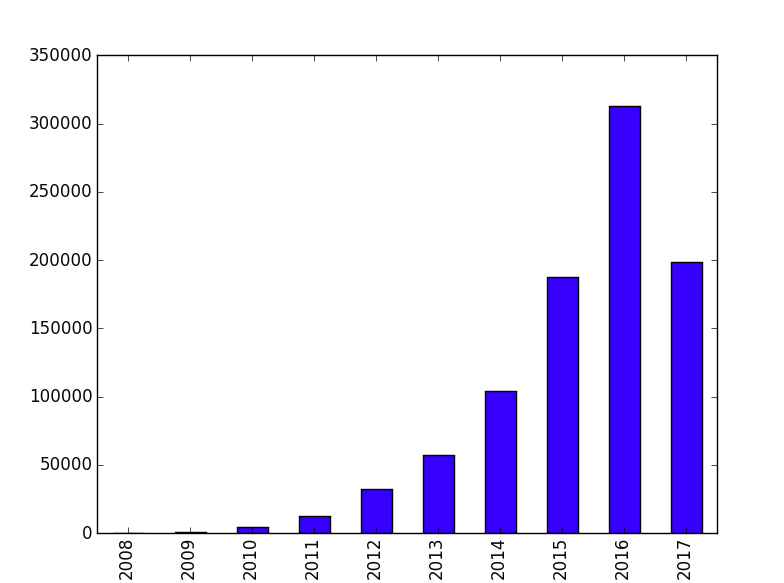
\includegraphics[width=\linewidth]{fig/fig1.png}
    \end{figure}

    La deuxième étape de l’étude s’intéresse à la place de l’environnement dans la communication des utilisateurs étudiés. Parmi les 1 110 utilisateurs qui composent le panel, 136 ont une mission liée à l’environnement. Toutefois, 763 utilisateurs ont publié au moins un tweet relatif à l’environnement, et 283 en ont publié au moins 10. La répartition en fonction des catégories d’organisations est présentée dans le Tableau \ref{table:15catenvir}. Les entreprises dont la mission est liée à la protection de l’environnement sont fortement représentées parmi les entreprises sociales. Cette partie émergente de l’ESS semble donc accorder un fort intérêt à ce secteur d’activité. A l’inverse, et de façon assez attendue, aucune mutuelle ni aucun organisme représentatif de l’ESS n’a une une activité environnementale. L’activité des mutuelles est réglementée et principalement tournée vers l’assurance et la santé. Le rôle des organismes représentatifs de l’ESS est de porter la voix de l’ensemble du secteur, dans toute la diversité de ses métiers. \\

    \begin{table}
    \caption{Dimension environnementale par type de compte }
    \label{table:15catenvir}
    \footnotesize

        \begin{tabularx}{\linewidth}{|X|r|r|r|r|r|r|}
        \hline
        \multirow{2}{*}{\textbf{Catégorie}} &	Comptes&	\multicolumn{2}{|X|}{\textbf{Comptes environnementaux}}	&
        Tweets&
        \multicolumn{2}{|X|}{\textbf{Tweets relatifs à l’environnement}} \\ \cline{2-7}
        &(Nombre)&\textbf{(Nombre)}&	\textbf{(\%)}
        &(Nombre*)&\textbf{(Nombre)}	&\textbf{(\% Moyen)} \\ \hline

        Association	&590&	80&	13.56&	522499&	13220&2.42 \\ \hline
        Autre	&26&	2&	7.69&	27439 &330	&1.65 \\ \hline
        Coopérative	&211&	21	&9.95&	129558& 2839&	2.35 \\ \hline
        Entreprise sociale	&75&	20&	26.67&	52135&2631&	5.55 \\ \hline
        Fondation	&115&	13&	11.30&	103268 & 3479&	2.53 \\ \hline
        Mutuelle	&67&	0&	0&	55998&475	&0.82 \\ \hline
        Fédérations - Organisme repr. & 26 &0 &0 &16896&247&1.35 \\ \hline
        \textbf{Total} &	\textbf{1110} &	\textbf{136} &	\textbf{12,25} &	\textbf{907793} &	\textbf{23221}& \\ \hline

        \end{tabularx}
        *Après exclusion des tweets répétés
    \end{table}




    Pour comparer les différents types d’entreprises indépendamment de leur activité environnementale ou non, nous nous intéressons au pourcentage de tweets ayant trait à l’environnement pour les organisations n’ayant pas une activité environnementale. Les données sont présentées dans le Tableau \ref{table:dimenenvirtypecomptenonenvir}. Exclusion faite des entreprises environnementales, le discours sur l’écologie est porté en premier lieu par les entreprises sociales (2,24 \% des tweets). Les coopératives et les utilisateurs de la catégorie « autre » consacrent plus de 1,5 \% de leurs publications aux sujets environnementaux. A l’opposé, les associations et mutuelles ont moins de 1 \% de tweets traitant des enjeux écologiques. \\


    \begin{table}
    \caption{Dimension environnementale des organisations non environnementales}
    \label{table:dimenenvirtypecomptenonenvir}
    \footnotesize

        \begin{tabularx}{\linewidth}{|X|r|r|r|r|r|r|}
        \hline

        \multirow{2}{*}{\textbf{Catégorie}}
        &\textbf{Comptes}
        &\textbf{Tweets}
        &\multicolumn{2}{|X|}{\textbf{Tweets environnementaux}} \\ \cline{2-5}

        &\textbf{(Nombre)}
        &\textbf{(Nombre)}
        &\textbf{(Nombre)}
        &\textbf{(\% moyen)} \\ \hline

       Entreprise sociale &	55 &	39 560 &	808 &	2,24 \\ \hline
        Coopérative	& 190 &	115 320 &	1 578 &	1,57 \\ \hline
        Autre	& 24 &	25 541 &	273 &	1,51 \\ \hline
        Fédérations - Organisme repr.	& 26 &	16 896	&247	&1,35 \\ \hline
        Fondation	& 102 &	85 876 &	912&	1,15 \\ \hline
        Association	& 510 &	448 951&	4 735&	0,94 \\ \hline
        Mutuelle	& 67 &	55 998&	475&	0,82 \\ \hline

        \textbf{Total} &	\textbf{974} &	\textbf{788142} &	\textbf{9028} &	\textbf{} \\ \hline

        \end{tabularx}
    \end{table}

    Dans cette étude, nous nous intéressons à la structure du réseau des acteurs de l’ESS sur Twitter, puis nous étudions les tweets à caractère environnemental selon l’approche de l’exploration de données.

\section{Analyse générale du corpus}
    \subsection{Etude des communautés}

        Dans un premier temps, on s’intéresse à la constitution en réseau des \oess. La figure \ref{figure:reseaumentions} permet de visualiser les communautés constituées par les liens entre les utilisateurs. Sur cette carte, les nœuds (cercles) correspondent aux comptes d’utilisateurs, et les liens qui relient deux utilisateurs indiquent que l’un a été mentionné par l’autre dans un tweet. La taille des nœuds est liée au degré entrant, c’est à dire au nombre de fois où l’utilisateur a été mentionné par un autre compte. Un compte recevant beaucoup de mentions joue un rôle central dans sa communauté.

        \begin{figure}
            \caption{Visualisation des liens inter-entreprises (basée sur les mentions)}
            \label{figure:reseaumentions}
            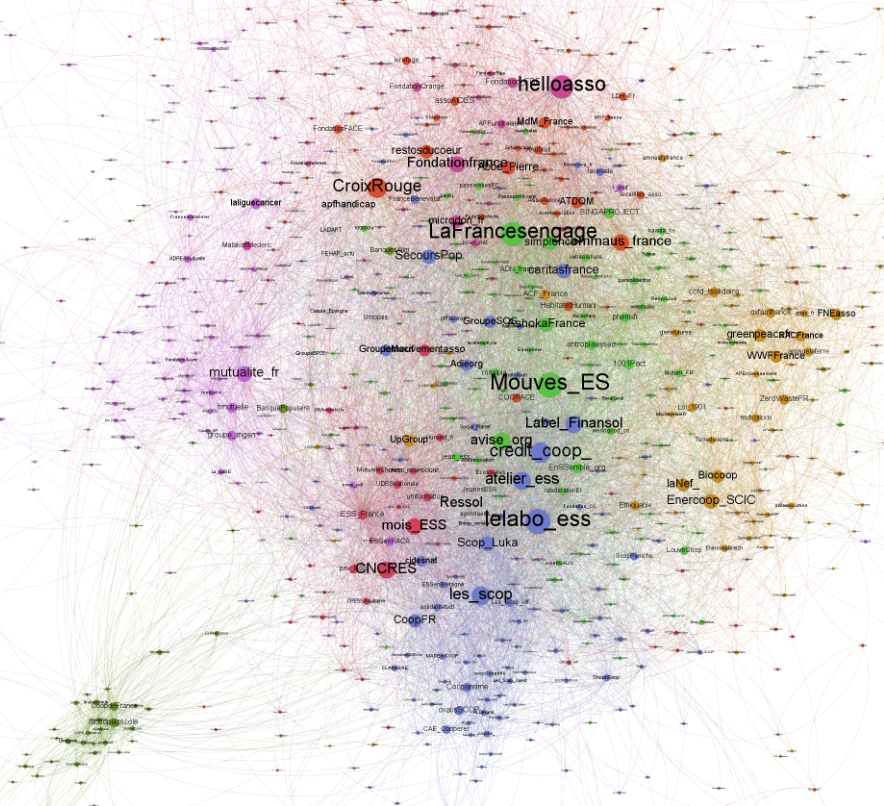
\includegraphics[width = \linewidth]{fig/fig2.png}
        \end{figure}

        Plusieurs communautés peuvent être mises en évidence. En bas à gauche (en vert), un groupe très distinct s’organise autour de Coop de France et la Coop Agricole (deux fédérations de coopératives agricoles). Autour, gravitent logiquement des coopératives agricoles, qui semblent former un réseau à part du reste de l’ESS.
        A gauche, en violet, un ensemble d’organisations s’organisent autour du compte de la Mutualité Française. Il s’agit essentiellement de mutuelles, mais aussi de fondations ou d’associations opérant dans le secteur de la santé, comme la Ligue Cancer et la Fondation de l’Avenir. Cette communauté se détache légèrement du reste de l’ESS mais laisse toutefois apparaître de nombreux liens avec d’autres groupes.
        En haut de la carte, deux communautés (en rouge et en rose) apparaissent très interconnectées. Il s’agit essentiellement de fondations et d’associations caritatives, organisées autour de l’entreprise HelloAsso (dont la mission est le financement de projets associatifs), de la Fondation de France (principale Fondation abritante en France) et d’entreprises symboliques du secteur non lucratif comme la Fondation Abbé Pierre, les Restos du Cœur, Emmaüs France, ou encore la Croix Rouge). Cette double communauté correspond donc au secteur de l’action sociale et de la solidarité.
        Sur la partie droite de la carte, en orange, une communauté se forme autour de la thématique de l’action environnementale. Deux sous-groupes se distinguent : le premier (en haut) autour de Green Peace, WWF France et France Nature Environnement ; le second autour de Enercoop (fournisseur d’énergie issue de sources renouvelables), Biocoop (épiceries bio) et la Nef (coopérative bancaire). Le premier groupe correspond à une action directe pour protéger l’environnement, quand le second propose des modes de consommation alternatifs pour limiter l’impact sur l’environnement.
        En bas de la carte (en bleu), des entreprises essentiellement coopératives s’organisent autour d’organismes de fédération et de promotion de l’ESS comme Le Labo ESS, Le mouvement des SCOP, Coop FR (qui anime le mouvement coopératif en France) ou encore l’Atelier ESS. Cette communauté est là aussi très interconnectée avec celle qui se trouve à sa gauche (rouge clair), qui fait apparaître d’autres instances représentatives comme le CNCRES, le Mois ESS, et ESS France (organisme institué par la loi ESS de 2014).
        Enfin, une communauté apparaît en position centrale, avec notamment de fortes interactions avec la communauté caritative, la communauté coopérative et la communauté environnementale. Elle s’organise autour d’organisations phares de l’entrepreneuriat social comme le \mouves, La France s’engage (label qui encourage les projets innovants), Ashoka France (association de promotion des entreprises sociales) et Avise (portail du développement de l’ESS). Il est intéressant de constater que cette communauté maintient des liens étroits avec trois groupes qui se distinguent nettement les uns des autres (le secteur caritatif, le secteur environnemental et le secteur coopératif). Ceci illustre le positionnement de l’entrepreneuriat social qui s’intéresse à tous les secteurs de l’ESS, mais se différencie plutôt par une démarche caractérisée par une démarche gestionnaire codifiée (avec notamment une grande proximité avec le milieu des startups), et un fort accent mis sur l’innovation. \\

        Une disposition similaire est observée avec une approche différente, dans laquelle les liens ne correspondent plus aux mentions mais aux abonnements (figure \ref{figure:reseauabos}). Ces liens sont pondérés. Pour deux utilisateurs A et B, le lien entre les deux a une valeur de 1 si A est abonné à B mais B n’est pas abonné à A, et une valeur de 2 si A et B sont mutuellement abonnés. Le fait de s’abonner à un utilisateur représente une action plus passive, puisqu’elle ne nécessite pas d’interaction : on indique simplement que l’on souhaite être informé des publications d’un utilisateur. C’est donc davantage un lien d’intérêt mutuel ou à sens unique.

        \begin{figure}
            \caption{Visualisation des liens inter-entreprises (basée sur les abonnements)}
            \label{figure:reseauabos}
            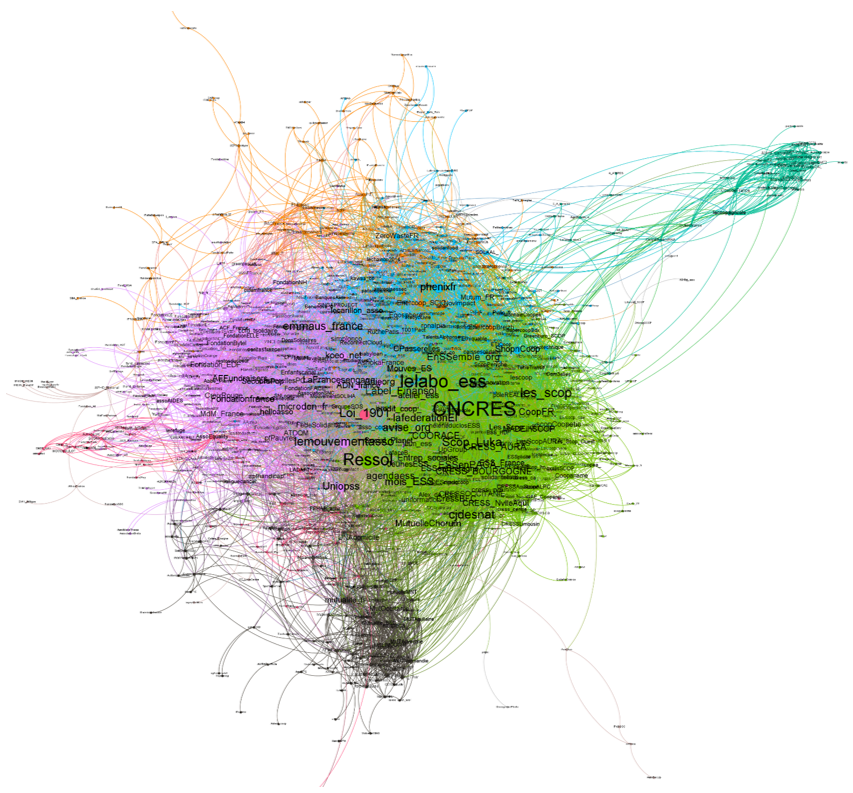
\includegraphics[width = \linewidth]{fig/fig3.png}
        \end{figure}

        La communauté des coopératives agricoles (en haut à droite) apparaît à nouveau très isolée du reste des utilisateurs qui forme un ensemble très interconnecté. Les mutuelles apparaissent en bas, formant également une communauté très homogène. Deux communautés majeures adoptent une position centrale sur la figure : la première (à droite, en vert) regroupe les organes de représentation de l’ESS, avec notamment le CNCRES, les CRESS et le Labo ESS. Le mouvement coopératif est intégré à cette communauté. A gauche, en violet, on retrouve la communauté ‘caritative’, qui regroupe fondations et associations ayant une forte mission sociale. Un sous-groupe de cette communauté se distingue à gauche : il s’agit d’organisations de lutte pour la tolérance et de défense des minorités, en particulier LGBT. Au-dessus, en bleu, la communauté des entrepreneurs sociaux, avec notamment de nombreuses startups assez jeunes (1001pact, Mutum, ShopnCoop, Pwiic…), semble à nouveau très ouverte, très connectée avec les autres groupes. La communauté ‘environnementale’ (en orange, en haut) se distingue moins nettement et tend à se confondre avec la communauté des entreprises sociales.

    \subsection{Statistiques multivariées}
        Afin de garantir la validité des résultats des deux régressions effectuées et de permettre la généralisation à une population, un certain nombre de critères doivent être respectés \parencite{field2009discovering}.
        Les variables explicatives de la régression sont continues, à l’exception de la variable ‘catégorie’ qui est catégorielle. Leur variance est non nulle. Toutes les valeurs de la variable expliquée sont indépendantes (chaque valeur correspond à un compte Twitter différent : c’est la raison pour laquelle le choix a été fait de ne considérer chaque compte qu’une seule fois en agrégeant les données de la période d’étude). La matrice des corrélations (tableau \ref{table:12correlations}) permet de vérifier l’absence de multicolinéarité parfaite. Le seul point d’attention relevé par ce test est la corrélation relativement importante entre le nombre de tweets avec mentions et le nombre de tweets avec un hashtag, qui invite à une interprétation prudente des coefficients correspondants. Les critères d’homoscédasticité et de distribution normale du terme d’erreur sont vérifiés visuellement grâce à la figure \ref{figure:5residus}. La distribution du terme d’erreur suit bien la structure d’une loi normale et la variance du test d’erreur ne dépend pas de la valeur prédite. Le résultat du test de Durbin-Watson est compris entre 1 et 3 et proche de 2 pour les deux modèles, ce qui garantit l’indépendance des termes résiduels. Enfin, les nuages de points confrontant les différentes variables du modèle suggèrent bien l’existence d’une relation linéaire qui justifie le recours à un modèle linéaire. Ainsi, le modèle semble donc approprié et généralisable à la population.

        \begin{landscape}

            \begin{table}
            \renewcommand{\arraystretch}{1.5}
            \begin{footnotesize}
                \caption{Matrice des corrélations}
                \label{table:12correlations}
                \begin{tabularx}{\linewidth}{|p{2cm}|X|X|X|X|X|X|X|X|X|}
                \hline
                &&\textbf{Nb\_ retweeted}&	\textbf{Nb\_ tw\_ hashtags}	&\textbf{nb\_ abonnements}	&\textbf{nb\_ abonnes}&	\textbf{nb\_ favoris}	&\textbf{nb\_ mentions}	&\textbf{nb\_ reponses}	&\textbf{nb\_ tweets}
                \\ \hline
                \multirow{2}{=}{\textbf{Nb\_ retweeted}}
                    &corr&1.000***&	0.400***&	0.121***&	0.699***&	0.879***&	0.291***&	0.171***&	0.291***\\
                    \cline{2-10}
                    &p-value&(0.000)&	(0.000)	&(0.000)&	(0.000)&	(0.000)	&(0.000)&	(0.000)&	(0.000)
                    \\ \hline
                \multirow{2}{=}{\textbf{Nb\_tw\_ hashtags}}
                    &corr&0.400***&	1.000***&	0.245***&	0.255***&	0.374***&	0.762***&	0.359***&	0.332***\\
                    \cline{2-10}
                    &p-value&(0.000)&	(0.000)	&(0.000)&	(0.000)	&(0.000)&	(0.000)	&(0.000)&	(0.000)
                    \\ \hline
                \multirow{2}{=}{\textbf{nb\_ abonnements}}
                    &corr&0.121***&	0.245***&	1.000***	&0.113***&	0.110***&	0.248***&	0.145***&	0.238***\\
                    \cline{2-10}
                    &p-value&	(0.000)&	(0.000)	&(0.000)	&(0.000)&	(0.000)&	(0.000)	&(0.000)&	(0.000)
                    \\ \hline
                \multirow{2}{=}{\textbf{nb\_abonnes}}
                    &corr&0.699***&	0.255***&	0.113***&	1.000***&	0.808***&	0.180***&	0.157***&	0.243***\\
                    \cline{2-10}
                    &p-value&(0.000)&	(0.000)	&(0.000)&	(0.000)&	(0.000)&	(0.000)&	(0.000)	&(0.000)
                    \\ \hline
                \multirow{2}{=}{\textbf{nb\_favoris}}
                    &corr&0.879***&	0.374***&	0.110***&	0.808***&	1.000***&	0.272***&	0.164***&	0.297***\\
                    \cline{2-10}
                    &p-value&(0.000)&	(0.000)&	(0.000)	&(0.000)&	(0.000)	&(0.000)&	(0.000)&	(0.000)
                    \\ \hline
                \multirow{2}{=}{\textbf{nb\_ mentions}}
                    &corr&0.291***&	0.762***&	0.248***&	0.180***&	0.272***&	1.000***&	0.699***&	0.356***\\
                    \cline{2-10}
                    &p-value&(0.000)&	(0.000)	&(0.000)&	(0.000)&	(0.000)	&(0.000)&	(0.000)	&(0.000)
                    \\ \hline
                \multirow{2}{=}{\textbf{nb\_ reponses}}
                    &corr&0.171***&	0.359***&	0.145***	&0.157***	&0.164***&	0.699***&	1.000***&	0.262***\\
                    \cline{2-10}
                    &p-value&(0.000)	&(0.000)&	(0.000)	&(0.000)&	(0.000)	&(0.000)&	(0.000)	&(0.000)
                    \\ \hline
                \multirow{2}{=}{\textbf{nb\_ tweets}}
                    &corr&0.291***&	0.332***&	0.238***&	0.243***&	0.297***&	0.356***&	0.262***&	1.000*** \\
                    \cline{2-10}
                    &p-value&(0.000)&	(0.000)	&(0.000)&	(0.000)	&(0.000)&	(0.000)	&(0.000)&	(0.000)
                    \\ \hline

                \end{tabularx}
            \end{footnotesize}
            \end{table}
        \end{landscape}


        \begin{landscape}
        \begin{figure}
            \caption{Hétéroscédasticité et normalité des résidus}
            \label{figure:5residus}
            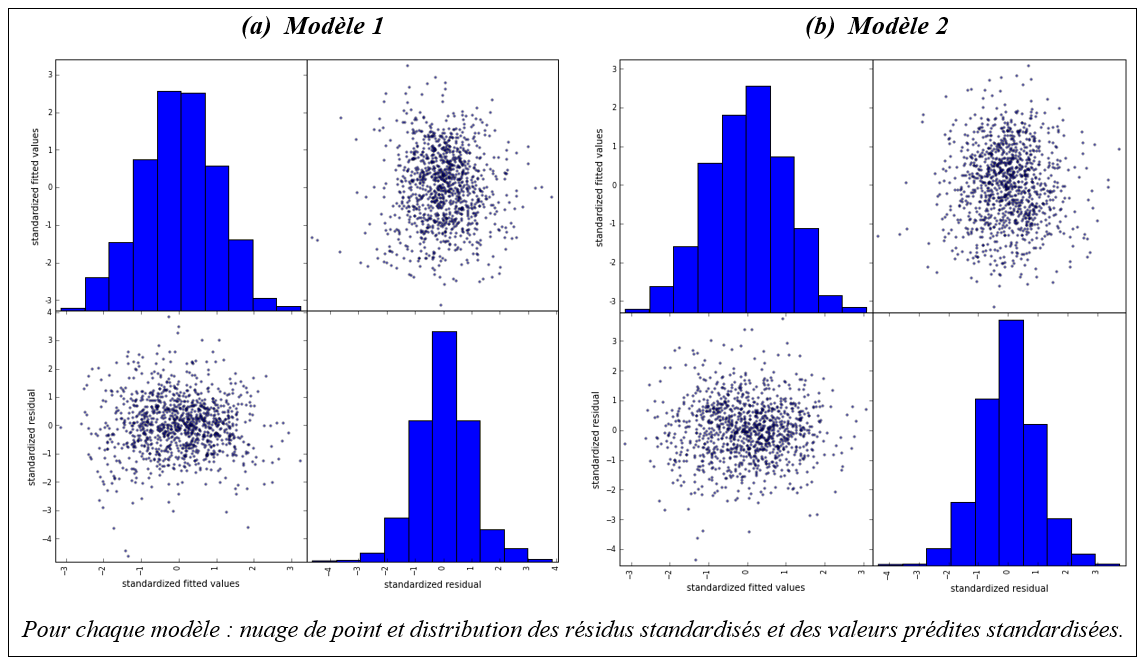
\includegraphics[width = \linewidth]{fig/fig5.PNG}
        \end{figure}
        \end{landscape}


        \begin{table}
        \caption{Résultats de la régression - modèle 1}
        \label{table:13regress1}
            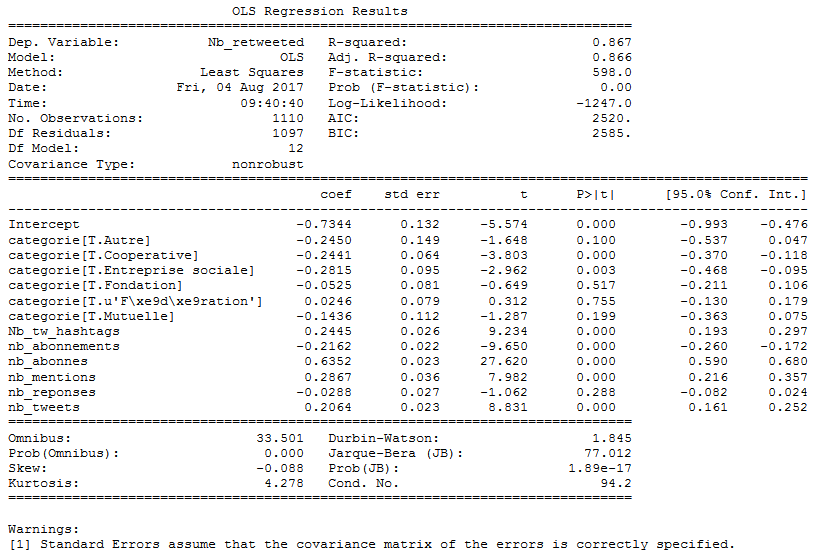
\includegraphics[width = \linewidth]{fig/tbl_regress1.png}
        \end{table}

        \begin{table}
        \caption{Résultats de la régression - modèle 2}
        \label{table:13regress2}
            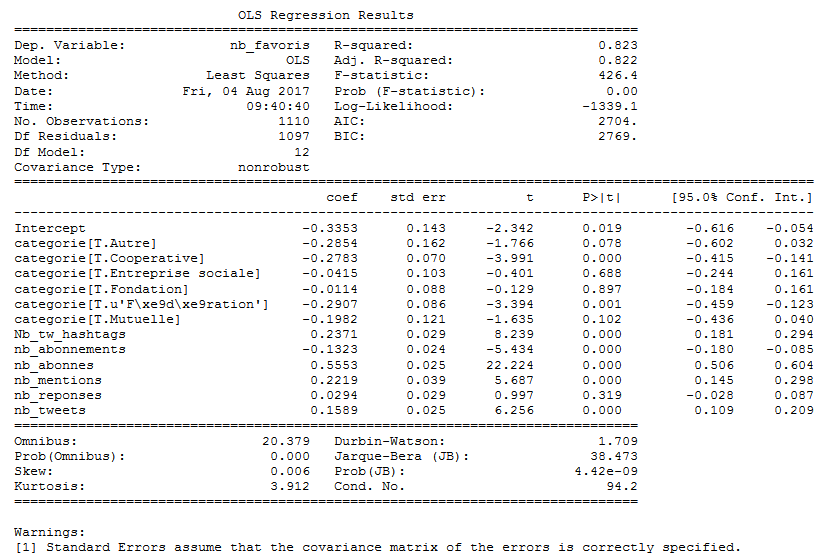
\includegraphics[width = \linewidth]{fig/tbl_regress2.png}
        \end{table}


        Les deux modèles (tableau \ref{table:13regress1} pour le nombre de retweets et \ref{table:13regress2} pour le nombre de favoris) présentent un fit ($R^2$) supérieur à 0.8 et sont donc très satisfaisants. Ils convergent globalement avec les résultats de Guo et Saxton. Tout d’abord, les résultats montrent que le niveau d’attention d’un compte est positivement associé au nombre d’abonnés, aussi bien pour le nombre de retweets que le nombre de favoris. Les coefficients associés (0.64 et 0.56 resp.) soulignent l’importance de cette donnée dans l’attention reçue par un compte. Le nombre de tweets publiés est un facteur relativement moins important, mais néanmoins très significatif de l’attention reçue. Le nombre de réponses faites à d’autres utilisateurs impacte positivement le nombre de favoris, mais négativement le nombre de retweets. Cependant, ce résultat est à prendre avec précautions, car les intervalles de confiance de 95\% prennent à la fois des valeurs positives et négatives pour les deux modèles. En réalité, l’influence du nombre de réponses est significative, mais très proche de zéro et n’est donc pas déterminante. En revanche, le nombre de tweets incluant au moins un hashtag impacte positivement le nombre de retweets et le nombre de favoris obtenus par un compte. Contrairement à Guo et Saxton, les deux modèles suggèrent qu’il existe bien un impact positif du nombre de tweets mentionnant un autre utilisateur sur l’attention obtenue. Par ailleurs, l’étude apporte un nouveau résultat intéressant : le nombre d’abonnements est négativement lié à l’attention obtenue. Enfin, de façon assez imprévisible, le fait d’être une coopérative a un impact négatif sur l’attention reçue pour les deux indicateurs. Appartenir au groupe des entreprises sociales impacte aussi négativement le nombre de retweet, et à celui des fédérations réduit le nombre de favoris.


    \subsection{Place du discours environnemental}

        Parmi les 1 110 utilisateurs qui composent le panel, 136 ont une mission liée à l’environnement. Toutefois, 763 utilisateurs ont publié au moins un tweet relatif à l’environnement et le nombre total de tweets environnementaux s’élève à 23 221. La répartition en fonction des catégories d’organisations est présentée dans le tableau \ref{table:15catenvir}.

        % \begin{table}
        % \caption{Catégorie de comptes et dimension environnementale }
        % \label{table:15catenvir}
        % \footnotesize

        %     \begin{tabularx}{\linewidth}{|l|r|r|r|r|r|}
        %     \hline
        %     \multirow{2}{*}{\textbf{Catégorie}} &	\multirow{2}{*}{\textbf{Effectif total}} &	\multicolumn{2}{|X|}{\textbf{Organisations environnementales}}	& \multicolumn{2}{|X|}{\textbf{Tweets relatifs à l’environnement}} \\ \cline{3-6}
        %     &&\textbf{Nombre}&	\textbf{Pourcentage}	&\textbf{Nombre}	&\textbf{Pourcentage} \\ \hline

        %     Association	&544&	69&	12,68&	12666&	2.27 \\ \hline
        %     Coopérative	&191&	21	&10,99&	2558&	2.28 \\ \hline
        %     Entreprise sociale	&73&	20&	27,40&	2573&	6.34 \\ \hline
        %     Fondation	&114&	13&	11,40&	3399&	1.87 \\ \hline
        %     Fédération	&111&	9&	8,11&	2935&	3.48 \\ \hline
        %     Autre	&27&	4&	14,81&	467	&2.23 \\ \hline
        %     Mutuelle	&50&	0&	0&	290	&0.55 \\ \hline
        %     \textbf{Total} &	\textbf{1110} &	\textbf{136} &	\textbf{12,36} &	\textbf{24888} &	\textbf{2.73} \\ \hline

        %     \end{tabularx}

        % \end{table}

        \subsubsection{Lien entre activité environnementale et discours environnemental}
        Bien que les organisations environnementales ne soient pas les seules à publier des tweets en lien avec ces questions, il est très probable qu’elles adoptent un discours plus fortement lié à l’environnement. Pour le vérifier, nous comparons le pourcentage de tweets relatifs à l’environnement entre deux groupes : les utilisateurs dont l’activité concerne l’environnement et ceux dont l’activité est hors secteur environnemental. On étudie la variable Pc\_envir qui correspond au pourcentage de tweets concernant l’environnement pour chaque utilisateur. La normalité de cette variable est testée à l’aide du test de Shapiro-Wilk et du test de Kolmogorov-Smirnov. Comme le montre le tableau \ref{table:16normalite}, les résultats sont fortement significatifs et l’hypothèse de normalité est donc rejetée. \\


        \begin{table}
        \caption{Test de normalité de la variable Pc\_envir}
        \label{table:16normalite}
        \footnotesize

            \begin{tabularx}{\linewidth}{|K{2cm}|K{4cm}|C|C|C|C|}
            \hline
            \multicolumn{2}{|c|}{}&	\multicolumn{2}{c|}{\textbf{Shapiro-Wilk}} &	\multicolumn{2}{c|}{\textbf{Kolmogorov-Smirnov}}\\ \cline{3-6}
            \multicolumn{2}{|c|}{}&\textbf{Stat}&	\textbf{p-value}	&\textbf{stat}	&\textbf{p-value} \\ \hline

            \multirow{3}{*}{Pc\_envir}
                &Ensemble des entreprises &	0.885 &	0.000 &	0.500 &	0.0\\ \cline{2-6}
                &Activité non liée à l’environnement &	0.876 &	0.000 &	0.500 &	0.0\\ \cline{2-6}
                &Activité liée à l’environnement &	0.966 &	0.002 &	0.529 &	0.0\\ \hline


            \end{tabularx}

        \end{table}

        Pour comparer les deux groupes, un test non paramétrique est donc utilisé : celui de Wilcoxon. Ce test repose sur un classement des individus du panel en fonction du classement des données, et non en fonction des données elles-mêmes : par conséquent il ne dépend pas de la distribution des variables étudiées \parencite{field2009discovering}. L’application du test nécessite de comparer deux échantillons de même taille, or l’échantillon n’est pas équitablement réparti entre les deux groupes. Le test est donc réalisé sur une sélection aléatoire de 100 individus au sein de chaque groupe. Le résultat est significatif au seuil de 1\% (tableau \ref{table:16wilcoxon}).

        \begin{table}
        \centering
        \caption{Résultats du test de Wilcoxon}
        \label{table:16wilcoxon}
            \begin{tabular}{|l|c|c|}
            \hline
            &\multicolumn{2}{|c|}{Wilcoxon} \\ \cline{2-3}
            & Stat & p-value \\ \hline
            Variable Pc\_envir & 253.0	& 0.000 \\ \hline
            \end{tabular}
        \end{table}

        Le test est renouvelé à plusieurs reprises avec un sous-échantillon différent et aboutit toujours à un résultat similaire. Comme escompté, les entreprises dont l’activité est liée à l’environnement ont donc un discours plus orienté vers les questions qui s’y rattachent que les entreprises dont le métier ne concerne pas l’écologie .



        \subsubsection{Lien entre type de compte d’utilisateur et discours environnemental}
        Comme le montre le tableau \ref{table:15catenvir}, les entreprises environnementales sont principalement représentées parmi les entreprises sociales et au sein de la catégorie ‘autre’. Au contraire, parmi les mutuelles, aucune n’est dédiée à l’environnement, leur secteur d’activité étant légalement restreint à l’assurance et la santé. \\

        Une comparaison de la proportion de tweets à caractère environnemental entre les différentes catégories peut être effectuée. Là encore, en raison de la non-normalité des variables, un test non-paramétrique, celui de Kruskal-Wallis est réalisé. Son fonctionnement est similaire à celui de Wilcoxon, mais généralisable à plus de deux groupes. Quel que soit le critère retenu, le test est significatif au seuil de 5\% suggérant qu’au moins l’une des catégories a un pourcentage de tweet relatifs à l’environnement significativement différent des autres (tableau \ref{table:17KW}). Pour déterminer laquelle, on effectue des comparaisons deux à deux entre les 8 groupes, ce qui nous conduit à effectuer 28 tests. \\


        \begin{table}
        \centering
        \caption{Résultats du test de Kruskal-Wallis}
        \label{table:17KW}
            \begin{tabular}{|l|c|c|}
            \hline
            &\multicolumn{2}{|c|}{Wilcoxon} \\ \cline{2-3}
            & Stat H & p-value \\ \hline
            Pc\_envir\_crit1	& 33.2416	& 0.000\\ \hline
            Pc\_envir\_crit2	& 55.4461	& 0.000\\ \hline
            Pc\_envir\_crit3	& 57.4710	& 0.000\\ \hline

            \end{tabular}
        \end{table}


        Conformément à ce qui est recommandé par \textcite{field2009discovering}, le test de Mann-Whitney est utilisé pour ces comparaisons deux à deux et la correction de Bonferoni est appliquée afin de limiter le taux d’erreur de Type 1. Ainsi, on évalue la qualité du test en divisant la valeur critique par le nombre de tests réalisés. Par conséquent, les résultats seront jugés significatifs au seuil de 5\% si la p-value est inférieure à 0.05/21 et au seuil de 1\% si la p-value est inférieure à 0.01/21. Les résultats présentés dans le tableau \ref{table:19MW} prennent en compte cette correction. \\

        \begin{table}
            \caption{Résultats des tests de Mann-Whitney – tous comptes d’utilisateurs}
            \label{table:19MW}
            \scriptsize

            \begin{tabularx}{\linewidth}{|l|K{0.4cm}|L|L|L|L|L|L|L|}
            \hline
            &&Association	& Autre	& Coopérative	& Entreprise Sociale	& Fondation& 	Fédération	& Mutuelle \\ \hline

            Association	&U&	147968&	5530&	45371&	12108***&	28299&	22515***&	11835 \\
        	    &P	&(0.5000)&	(0.0131)&	(0.0038)&	(0.0000)&	(0.0663)&	(0.0000)&	(0.0589)\\ \hline

            Autre&	U&	5530&	364&	2313&	790&	1222&	1493&	379\\
            	&P&	(0.0131)	&(0.4965)&	(0.1903)&	(0.0645)&	(0.0470)&	(0.4893)&	(0.0006)\\ \hline

            Coopérative&	U&	45371&	2313&	18240&	4992**	&10168	&9404	&3430\\
            	&P&	(0.0038)&	(0.1903)&	(0.4998)&	(0.0002)&	(0.1640)&	(0.0494)&	(0.0009)\\ \hline

            Entreprise Sociale&	U&	12108***&	790&	4992**&	2664	&2662***&	3272&	798***\\
            &	P&	(0.0000)&	(0.0645)&	(0.0002)&	(0.4992)&	(0.0000)&	(0.0136)&	(0.0000)\\ \hline

            Fondation&	U&	28299&	1222&	10168&	2662***	&6498&	5031&	2190\\
            &	P&	(0.0663)&	(0.0470)&	(0.1640)&	(0.0000)&	(0.4996)&	(0.0038)&	(0.0082)\\ \hline

            Fédération - Org. Repr.&	U&	22515***&	1493&	9404&	3272&	5031&	6160&	1570***\\
            &	P&	(0.0000)&	(0.4893)&	(0.0494)&	(0.0136)&	(0.0038)&	(0.4996)&	(0.0000)\\ \hline

            Mutuelle&	U&	11835&	379&	3430&	798***&	2190&	1570***&	1250\\
            &	P&	(0.0589)&	(0.0006)&	(0.0009)&	(0.0000)&	(0.0082)&	(0.0000)&	(0.4980)\\ \hline

            \end{tabularx}
        \end{table}

        \begin{table}
            \caption{Résultats des tests de Mann-Whitney – hors organisations environnementales}
            \label{table:20MWbis}
            \scriptsize

            \begin{tabularx}{\linewidth}{|l|K{0.4cm}|L|L|L|L|L|L|L|}
            \hline
            &&Association	& Autre	& Coopérative	& Entreprise Sociale	& Fondation& 	Fédération	& Mutuelle \\ \hline


                Association			&U&	112812	&   	3806	&	33136**	&	7029***	&	20738	&	16115***&	11687\\
                					&p&	(0.5000)&   	(0.0053)&	(0.0002)&	(0.0000)&	(0.0133)&	(0.0000)&	(0.4240)\\ \hline
                Autre				&U&	3806	&   	264	&       1750&		511		&	916		&	1149	&	375     \\
                					&p&	(0.0053)&   	(0.4956)&	(0.2027)&	(0.1330)&	(0.0550)&	(0.4402)&	(0.0074)\\ \hline
                Coopérative			&U&	33136**	&   	1750	&	14450	&	3324	&	7926	&	7518	&	3346\\
                					&p&	(0.0002)&   	(0.2027)&	(0.4998)&	(0.0017)&	(0.1408)&	(0.0315)&	(0.0095)\\ \hline
                Entreprise Sociale	&U&	7029***	&   	511		&	3324	&	1404	&	1705**	&	2296	&	672***\\
                					&p&	(0.0000)&   	(0.1330)&	(0.0017)&	(0.4987)&	(0.0001)&	(0.0616)&	(0.0000)\\ \hline
                Fondation			&U&	20738	&   	916		&	7926	&	1705**	&	5100	&	3900	&	2146\\
                					&p&	(0.0133)&   	(0.0550)&	(0.1408)&	(0.0001)&	(0.4995)&	(0.0013)&	(0.0628)\\ \hline
                Fédération - Org. repr.			&U&	16115***&   	1149	&	7518	&	2296	&	3900	&	5202	&	1567**\\
                					&p&	(0.0000)&   	(0.4402)&	(0.0315)&	(0.0616)&	(0.0013)&	(0.4995)&	(0.0000)\\ \hline
                Mutuelle			&U&	11687	&   	375		&	3346	&	672***	&	2146	&	1567**	&	1250\\
                					&p&	(0.4240)&   	(0.0074)&	(0.0095)&	(0.0000)&	(0.0628)&	(0.0000)&	(0.4986)\\ \hline


            \end{tabularx}
        \end{table}


        Ces tests montrent que les entreprises sociales consacrent un pourcentage de tweets à l’environnement significativement plus élevé que les associations, fondations et mutuelles (seuil de 1\%) et que les coopératives (seuil de 5\%). A l’opposé, les associations et mutuelles publient moins de tweets relatifs à l’environnement que les fédérations. Toutefois, ce résultat peut être influencé par la proportion importante d’entreprises sociales qui ont une activité environnementale et qui donc publient davantage de tweets relatifs à l’écologie. Inversement, les associations environnementales sont « noyées » dans une masse d’organisations ayant des missions différentes. Pour neutraliser cet impact, les tests sont reproduits sur l’échantillon après élimination des utilisateurs liés à l’environnement (N = 974). Les résultats sont très similaires, voire plus significatifs (tableau \ref{table:20MWbis}). La différence est particulièrement marquée entre d’un côté les coopératives et entreprises sociales, et de l’autre les associations. Les entreprises sociales publient aussi davantage de tweets concernant l’environnement que les fondations et mutuelles. Le discours environnemental semble donc plutôt adopté par des entreprises de l’ESS ayant des caractéristiques proches des entreprises classiques .

\section{Exploration de texte}
    \subsection{Extraction des thématiques principales}
        Trois algorithmes sont utilisés pour faire émerger des catégories thématiques à partir des mots du corpus. L’algorithme NMF avec la norme de Frobenius donne les meilleurs résultats. Six thématiques sont mises en évidence (pour n=5, les catégories sont peu lisibles ; à partir de n=7, des catégories non porteuses de sens apparaissent). Les éléments les plus significatifs sont présentés dans le Tableau \ref{table:thematiquesemergentes}.

        \begin{scriptsize}
        \renewcommand*{\arraystretch}{0.8}
        \begin{longtable}{
            |>{\setlength{\baselineskip}{0.7\baselineskip}}K{0.14\textwidth}
            |>{\setlength{\baselineskip}{0.7\baselineskip}}K{0.14\textwidth}
            |>{\setlength{\baselineskip}{0.7\baselineskip}}K{0.14\textwidth}
            |>{\setlength{\baselineskip}{0.7\baselineskip}}K{0.14\textwidth}
            |>{\setlength{\baselineskip}{0.7\baselineskip}}K{0.14\textwidth}
            |>{\setlength{\baselineskip}{0.7\baselineskip}}K{0.14\textwidth}
            | }
            \caption{Thématiques émergentes}
            \label{table:thematiquesemergentes} \\ \hline

            1 - Climat	&	2 - Pollution	&	3 - Recyclage	&	4 - Agriculture 	&	5 - Energie	&	6 - Biodiversité	\\ \hline
            \endfirsthead \hline
            1 - Climat	&	2 - Pollution	&	3 - Recyclage	&	4 - Agriculture 	&	5 - Energie	&	6 - Biodiversité	\\
            \multicolumn{6}{|c|}{(Suite)} \\ \hline
            \endhead

            \cellcolor{blue!25}climat (6.72)	&	\cellcolor{blue!25}pollution (4.99)	&	\cellcolor{blue!25}recyclage (3.28)	&	\cellcolor{blue!25}bio (6.01)	&	\cellcolor{blue!25}énergie (6.19)	&	\cellcolor{blue!25}biodiversité (5.86)	\\

            \cellcolor{blue!25}cop21 (3.76)	&	\cellcolor{blue!25}air (2.95)	&	\cellcolor{blue!25}economiecirculaire (2.55)	&	\cellcolor{blue!25}agriculture (1.74)	&	\cellcolor{blue!25}renouvelable (1.14)	&	\cellcolor{blue!25}loup (0.86)	\\

            \cellcolor{blue!25}climatique (0.89)	&	\cellcolor{blue!25}polluant (1.45)	&	\cellcolor{blue!25}déchets (2.28)	&	\cellcolor{blue!25}local (0.54)	&	\cellcolor{blue!25}nucléaire (0.82)	&	\cellcolor{blue!25}nature (0.85)	\\

            \cellcolor{blue!25}charbon (0.58)	&	\cellcolor{blue!25}iledefrance (1.43)	&	ess (2.24)	&	\cellcolor{blue!25}biologique (0.53)	&	économie (0.76)	&	\cellcolor{blue!25}anb2016 (0.71)	\\

            \cellcolor{blue!25}accord (0.53)	&	\cellcolor{blue!25}épisode (1.25)	&	projet (1.62)	&	\cellcolor{blue!25}alimentation (0.48)	&	\cellcolor{blue!25}enr (0.57)	&	\cellcolor{blue!25}canislupus (0.54)	\\

            \cellcolor{blue!25}changement (0.52)	&	pm10 (1.23)	&	durable (1.54)	&	\cellcolor{blue!25}pesticides (0.4)	&	\cellcolor{blue!25}enercoop (0.44)	&	\cellcolor{blue!25}ouiauxloups (0.5)	\\

            \cellcolor{blue!25}paris (0.51)	&	attention (1.13)	&	nouveau (1.36)	&	conférence (0.29)	&	\cellcolor{blue!25}solaire (0.44)	&	ateliercoecolo (0.44)	\\

            agir (0.39)	&	prévoir (1.13)	&	transition (1.35)	&	\cellcolor{blue!25}produit (0.28)	&	\cellcolor{blue!25}électricité (0.38)	&	loi (0.38)	\\
            pr (0.34)	&	santé (0.61)	&	social (1.32)	&	\cellcolor{blue!25}bon (0.27)	&	\cellcolor{blue!25}transitionenergetique (0.35)	&	agriculture (0.24)	\\
            devoir (0.34)	&	idf (0.49)	&	écolo (1.31)	&	\cellcolor{blue!25}manger (0.25)	&	positif (0.34)	&	royalsegolene (0.22)	\\
            tout (0.29)	&	\cellcolor{blue!25}episode (0.48)	&	découvrir (1.2)	&	\cellcolor{blue!25}biocoop (0.25)	&	france (0.33)	&	france (0.21)	\\
            mobilisation (0.28)	&	\cellcolor{blue!25}particule (0.43)	&	merci (1.08)	&	\cellcolor{blue!25}agroécologie (0.24)	&	citoyen (0.31)	&	français (0.19)	\\
            dire (0.27)	&	\cellcolor{blue!25}airparif (0.37)	&	\cellcolor{blue!25}zerowaste (0.81)	&	rdv (0.21)	&	\cellcolor{blue!25}fossile (0.31)	&	eau (0.18)	\\
            \cellcolor{blue!25}réchauffement (0.27)	&	constater (0.35)	&	dd (0.77)	&	découvrir (0.18)	&	\cellcolor{blue!25}énergétique (0.3)	&	agence (0.17)	\\
            santé (0.26)	&	\cellcolor{blue!25}qualité (0.28)	&	paris (0.76)	&	\cellcolor{blue!25}producteur (0.18)	&	\cellcolor{blue!25}consommation (0.29)	&	\cellcolor{blue!25}protection (0.17)	\\
            conférence (0.26)	&	\cellcolor{blue!25}paris (0.27)	&	france (0.75)	&	nouveau (0.18)	&	\cellcolor{blue!25}edf (0.23)	&	national (0.16)	\\
            engager (0.26)	&	\cellcolor{blue!25}atmosphérique (0.19)	&	énergétique (0.74)	&	coopérative (0.17)	&	damienhasbroucq (0.22)	&	\cellcolor{blue!25}chasse (0.14)	\\
            \cellcolor{blue!25}cop22 (0.26)	&	faible (0.18)	&	développement (0.74)	&	\cellcolor{blue!25}équitable (0.17)	&	promotelec (0.21)	&	note (0.13)	\\
            racfrance (0.26)	&	\cellcolor{blue!25}pic (0.18)	&	\cellcolor{blue!25}déchet (0.73)	&	petit (0.17)	&	\cellcolor{blue!25}energie (0.2)	&	préserver (0.12)	\\
            action (0.26)	&	lt (0.17)	&	\cellcolor{blue!25}ateliercoecolo (0.71)	&	semaine (0.15)	&	parler (0.2)	&	nouveau (0.12)	\\
            engagement (0.24)	&	savoir (0.17)	&	tout (0.68)	&	santé (0.15)	&	transition (0.19)	&	agir (0.11)	\\
            solution (0.23)	&	ville (0.15)	&	économie (0.61)	&	ligne (0.15)	&	\cellcolor{blue!25}renouvelables (0.18)	&	protéger (0.11)	\\
            monde (0.22)	&	france (0.14)	&	solidaire (0.61)	&	magasin (0.14)	&	\cellcolor{blue!25}transitionénergétique (0.18)	&	projet (0.11)	\\
            alimentation (0.21)	&	intérieur (0.14)	&	\cellcolor{blue!25}recycler (0.57)	&	cantine (0.14)	&	amorce (0.18)	&	\cellcolor{blue!25}biocentrisme (0.11)	\\
            pouvoir (0.2)	&	an (0.13)	&	parler (0.55)	&	solidaire (0.14)	&	vert (0.17)	&	sauver (0.1)	\\
            \cellcolor{blue!25}climatechange (0.2)	&	voiture (0.13)	&	citoyen (0.52)	&	tout (0.13)	&	europe (0.16)		& coprae (0.1)	\\
            agriculture (0.19)	&	fin (0.13)	&	entreprise (0.52)	&	beau (0.13)	&	logement (0.16)	&	merci (0.1)	\\
            nouaillas (0.19)	&	enfant (0.13)	&	soutenir (0.49)	&\cellcolor{blue!25}	filière (0.12)	&	grâce (0.16)	&	journée (0.09)	\\
            olivier (0.19)	&	lutter (0.12)	&	sport (0.49)	&\cellcolor{blue!25}	agricole (0.12)	&	français (0.15)	&	vidéo (0.09)	\\
            clubpresselyon (0.19)	&	moyen (0.11)	&	cc (0.49)	&	\cellcolor{blue!25}culture (0.12)	&	\cellcolor{blue!25}éolien (0.15)	&	toulouse (0.09)	\\
            impact (0.19)	&	monde (0.1)	&	pouvoir (0.46)	&	merci (0.12)	&	central (0.15)	&	métier (0.09)	\\
            sauver (0.19)	&	million (0.09)	&	\cellcolor{blue!25}tri (0.46)	&	samedi (0.12)	&	focus (0.15)	&	prix (0.09)	\\
            jour (0.18)	&	effet (0.09)	&	impact (0.45)	&	vidéo (0.12)	&	hespul (0.15)	&	site (0.08)	\\
            pays (0.17)	&	danger (0.09)	&	responsable (0.44)	&	jardin (0.12)	&	choisir (0.14)		& urbain (0.08)	\\
            enjeu (0.17)	&	mesure (0.08)	&	innovation (0.42)	&	france (0.12)	&	accès (0.14)	&	assise (0.08)	\\
            lemondefr (0.17)	&	personne (0.07)	&	atelier (0.42)	&	salon (0.11)	&	passer (0.12)	&	\cellcolor{blue!25}animal (0.08)	\\
            france (0.17)	&	victime (0.07)	&	économique (0.4)	&	\cellcolor{blue!25}légume (0.11)	&	air (0.12)	&	enjeu (0.08)	\\
            face (0.17)	&	leparisien (0.07)	&	lafabriqueecolo (0.39)	&	\cellcolor{blue!25}ferme (0.1)	&	facture 0.12)	&	découvrir (0.08)	\\
            bnpparibas (0.16)	&	pesticides (0.07)	&	emploi (0.39)	&	web (0.1)	&	\cellcolor{blue!25}enercoopscic (0.11)	&	\cellcolor{blue!25}forêt (0.07)	\\
            négociation (0.16)	&	découvrir (0.07)	&	transitionenergetique (0.38)	&	français (0.1)	&	plein (0.11)	&	nantes (0.07)	\\ \hline

        \end{longtable}
        \end{scriptsize}

        La première catégorie thématique est celle du \textbf{climat}, marquée par la problématique du réchauffement climatique. Elle est fortement caractérisée par la COP21 et les accords internationaux pour le climat. Les tweets correspondant mettent l'accent sur l’action, la mobilisation et l’engagement nécessaires pour sauver la planète. Bien que le registre soit plutôt alarmiste, le terme de ‘solution’ suggère que les utilisateurs intervenants sur cette thématique proposent également des alternatives.

        La seconde catégorie correspond à la question de la \textbf{pollution}, de l’air comme des sols, en lien avec les enjeux de santé. Là aussi, le registre employé met l’accent sur le risque (‘attention’, ‘danger’, ‘victime’) et sur la lutte et la prévention.

        Une troisième catégorie tourne autour du\textbf{ recyclage des déchets}. Elle s’inscrit dans une perspective plus positive, plus constructive, faisant référence au développement durable (‘ dd’) et à la transition écologique et énergétique. Cette catégorie est directement rattachée à l’ESS dans sa dimension économique (notamment l’emploi et l’innovation) et solidaire.

        Le quatrième thème est celui de \textbf{l’agriculture et de l’alimentation}. Il fait référence à l’agriculture locale et biologique, au commerce équitable et renvoie au débat sur les pesticides. Cette thématique se rapproche de la précédente par le lien qui est fait avec la santé et la solidarité. Les adjectifs ‘beau’ et ‘bon’ indiquent un discours plutôt positif, tourné vers les alternatives plutôt que vers les risques.

        La cinquième thématique est celle de\textbf{ l’énergie}, sous l’angle des différents modes de production (nucléaire, solaire, éolien, ressources fossiles) mais aussi économiques (économie, logement, consommation, facture). L’accent est mis sur la responsabilité citoyenne et sur la possibilité de choisir (en référence au choix du fournisseur d’électricité). Là encore, cette catégorie est plutôt tournée vers les alternatives en s’inscrivant dans la transition énergétique.

        Enfin, la dernière catégorie est celle de la \textbf{biodiversité}, de la préservation de la nature. Elle est particulièrement marquée par la question des loups qui font l’objet de désaccords marqués entre écologistes, éleveurs et pouvoirs publics dans les régions où ils sont implantés. Le discours semble plutôt alarmiste : il s’agit de préserver, protéger, sauver.  Des alternatives apparaissent toutefois avec le ‘biocentrisme’. \\

        La technique de la classification non supervisée a permis de faire émerger six catégories thématiques distinctes. Cependant, il existe des interconnexions entre ces catégories, notamment autour de la santé, de l’agriculture, de l’énergie ou de l’engagement citoyen qui se retrouvent dans différentes catégories. L’ESS est donc présente sur les grandes thématiques écologiques actuelles. Cependant, seule la catégorie « recyclage » est directement liée à l’ESS et au développement durable.


    \subsection{Etude des stratégies rhétoriques}

        \subsubsection{Sentiment et objectivité}

            Dans la section précédente, nous avons identifié des thématiques, associées à différents registres. Certaines reposent plutôt sur une analyse des risques, quand d’autres sont tournées vers les solutions, les alternatives possibles.  Dans cette partie, nous classons les tweets selon qu’ils ont un caractère positif ou négatif (dimension « sentiment ») et objectif ou subjectif (dimension « objectivité »), à l’aide d’une méthode de classification supervisée : l’algorithme de Naives-Bayes. La fiabilité de l’algorithme est de 0.67 pour les deux dimensions, ce qui signifie que 67\% des tweets sont correctement classés. La répartition des tweets selon ces deux dimensions est plutôt équilibrée. Sur un total de 23 221 tweets à caractère environnemental, 11 645 sont identifiés comme négatifs et 11 576 comme positifs ; 10 399 sont objectifs et 12 822 subjectifs.

            Au moyen d’une Analyse Factorielle des Correspondances, on met en lien les dimensions du discours avec les utilisateurs ou les catégories d’utilisateurs. La synthèse des résultats est donnée en Figure \ref{fig:syntheseAFC} et une visualisation sur forme de cartes factorielles est proposée en Figure \ref{fig:AFCcategories} et Figure 6.

            \begin{figure}
                \caption{Synthèse de l'AFC}
                \label{fig:syntheseAFC}
                \fbox{
                    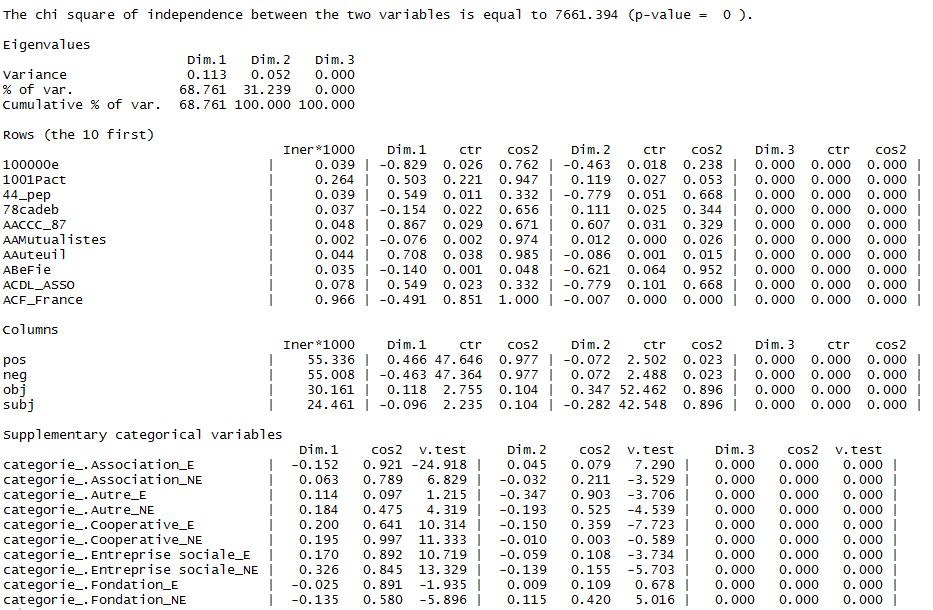
\includegraphics[width=\linewidth]{fig/AFC_summary.JPG}
                }
            \end{figure}

            Par construction, la variance est répartie sur deux axes, l’un correspondant au sentiment, l’autre à l’objectivité. L’axe horizontal (dimension 1) explique 68,76 \% de la variance totale et correspond au sentiment. Les organisations du corpus se distinguent donc principalement selon qu’elles ont recours à un discours majoritairement positif ou majoritairement négatif. L’axe vertical (dimension 2) explique les 32,24 \% de variance restante, qui correspondent à l’opposition entre les tweets objectifs et les tweets subjectifs. Cette distinction est donc nettement moins significative. La Figure \ref{fig:AFCcategories} présente une projection des catégories d’organisations sur ces deux axes. On a ici distingué pour chaque catégorie les organisations environnementales et les organisations non environnementales (ex : Association\_E vs Association\_NE). La qualité de projection est mesurée à l’aide du cosinus carré (cf. figure \ref{fig:syntheseAFC} : colonne cos2), compris entre 0 et 1.

            \begin{figure}
                \caption{Carte factorielle : catégories d'utilisateurs}
                \label{fig:AFCcategories}
                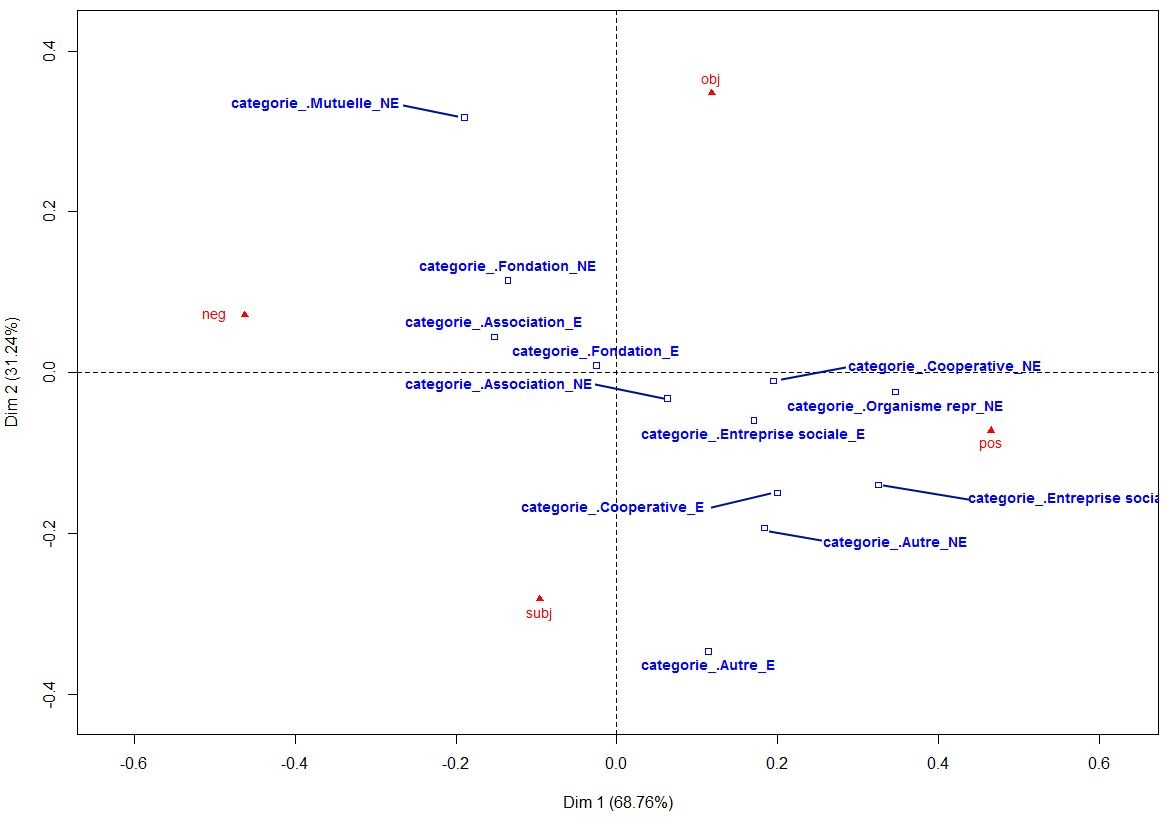
\includegraphics[width=\linewidth]{fig/AFC_categories.JPG}
            \end{figure}

            Les mutuelles se distinguent par un positionnement vers des tweets négatifs mais objectifs. Quelques exemples de tweets nous permettent de comprendre ce discours. Les mutuelles opèrent dans le secteur de la santé et de l’assurance. Par conséquent, elles abordent les thématiques environnementales sur l’angle des risques sanitaires, ceux-ci ayant un impact pour leurs bénéficiaires. L’augmentation des maladies liées à l’environnement pose aussi un risque économique en faisant augmenter les remboursements de frais de santé. Globalement, elles n’adoptent pas une position engagée, mais s’intéressent plutôt aux études publiées sur ces sujets.

            \begin{quotation}
             \citit{La pollution de l’environnement entraîne 1,7 million de décès d’enfants par an https://t.co/gXir1rrLgH} (Mutuelle Apreva, mars 2017)
            \end{quotation}

            A l’opposé, les organismes de représentation adoptent un discours très positif sur la question de l’écologie\footnote{Les valeurs correspondantes n’apparaissent pas sur la Figure 4 qui n’intègre que les 10 premières lignes. La qualité de projection est de 0.995 sur l’axe 1 et 0.005 sur l’axe 2.}. Ce résultat est toutefois à nuancer : cette catégorie représente un petit nombre d’organisations et le nombre de tweets ayant trait à l’environnement est réduit (247 tweets). Les publications concernent des appels à projets, des informations sur des évènements autour des questions environnementales (conférences, ateliers…) ou la valorisation de projets innovants. Ces organisations sont plutôt dans une démarche de promotion de l'\ess et de son action environnementale.

            \begin{quotation}
                \citit{ L'\#ESS s'engage pour la \#transitionénergétique citoyenne ... \#COP21 https://t.co/lGryBHgJnI} (\cress Limousin, décembre 2015) \\
                \citit{Lilo le moteur de recherche qui finance des projets sociaux et environnementaux que vous choisissez ! https://t.co/RZ9U9JsWB1} (\cress Champagne-Ardennes, juin 2016)
            \end{quotation}

            Les associations se distinguent essentiellement sur l’axe horizontal. Elles ont globalement une position centrale, peu discriminante, qui s’explique vraisemblablement par la grande diversité du secteur et donc des positionnements. Les associations environnementales se distinguent toutefois par un discours plus négatif. Elles ont souvent une position engagée, réagissant à l’actualité politique. Elles ont aussi un rôle d’alerte sur les risques environnementaux.

            \begin{quotation}
                \citit{\#Nucléaire: \@RoyalSegolene utilise la \#PPE pour relancer la filière \#MOX. Et les \#déchets, on en fait quoi? Non à l'enfouissement à \#Bure !} (Association amisdelaterre, juillet 2016)
            \end{quotation}

            Concernant les fondations dont la mission est liée à l’environnement, l’AFC ne permet pas d’identifier une stratégie distincte. En revanche, les fondations non environnementales adoptent, de façon similaire mais moins marquée que les mutuelles, un discours plutôt négatif mais objectif. De nombreuses fondations opérant dans le domaine de la santé, ce positionnement peut s’expliquer par les mêmes raisons.

            Un discours majoritairement positif est adopté par les coopératives et les entreprises sociales, qu’elles aient une mission environnementale ou non. Ces organisations se distinguent assez mal sur l’axe vertical, à l’exception des coopératives environnementales associées à un discours sensiblement plus subjectif. Dans le discours des coopératives et des entreprises sociales, l’accent est mis sur les aspects positifs. De nombreux tweets portent sur les avancées en matière environnementale, les progrès effectués, ainsi que les opportunités de développement. De nombreux cas de réussites entrepreneuriales basées sur les questions environnementales sont mis en avant, comme pour démontrer que les alternatives existent et qu’elles se mettent déjà en place. Les tweets jouent aussi un rôle de promotion des actions environnementales menées par les entreprises.

            \begin{quotation}
                \citit{Pr bien commencer 2016, voici 1 reportage d'1 école parisienne qui a déjà pris de bonnes résolutions. https://t.co/yYwNUr6Kcj \#biodéchets} (Entreprise Sociale loveyourwaste, janvier 2016) \\

                \citit{Les producteurs du \@groupedaucy en route vers l'\#Agroecologie \#sustainableagriculture https://t.co/hGqfJZzMaz } (groupedaucy, coopérative novembre 2016)
            \end{quotation}

            L’analyse des axes peut être facilitée par la visualisation des cas les plus significatifs. La figure \ref{fig:AFCentreprises} fait apparaitre les 30 comptes Twitter ayant la plus forte contribution à la construction des axes.

            Dans le cadran supérieur gauche, l’association Airparif se distingue par un discours objectif mais essentiellement négatif. Ce compte Twitter publie régulièrement une information sur le niveau de pollution en Ile de France… souvent élevé, mais qui relève d’une mesure parfaitement objective.  Plus bas, la Fondation du Souffle (\textit{FduSouffle}), qui rassemble des acteurs de la lutte contre les maladies respiratoires se distingue assez logiquement par un discours négatif, la pollution étant une des causes de ces maladies.

            Le cadre inférieur gauche fait apparaitre un groupe d’associations associées à un discours plutôt négatif, dont WWF France, Oxfam France (\textit{oxfam\_fr}), GreenPeace (\textit{greenpeacefr}) et Sortir du Nucléaire France (\textit{sdnfr}). Ces associations ont un rôle d’activisme sur les questions environnementales (à l’exception d’Oxfam qui lutte contre la pauvreté mais s’exprime aussi sur l’écologie). Elles adoptent parfois un rôle de lanceur d’alerte, en signalant les projets allant à l’encontre de la transition écologique et en alertant sur les dangers pour les citoyens. Ces organisations prennent fréquemment des positions politiques en lien avec l’actualité.


            \begin{quotation}
                \citit{Richesse et revenus extrêmes sont inefficaces économiquement et nuisent à l’environnement, selon 1 rapport http://t.co/xrtYothI} (Oxfam France, janvier 2013) \\
                \citit{Environnement: le programme \#Macron est incohérent et ne remet pas en cause le système actuel désastreux \#TelSonne https://t.co/iJgbPWaeCa} (GreenPeace France, avril 2017) \\
                \citit{Important rejet radioactif à centrale \#nucléaire de Golfech (82), déclaré presque 1 semaine + tard : notre réaction https://t.co/S8gUiHBxuE} (Sortir du Nucléaire France, octobre 2016)

            \end{quotation}


            \begin{figure}
                \caption{Carte factorielle : Utilisateurs significatifs}
                \label{fig:AFCentreprises}
                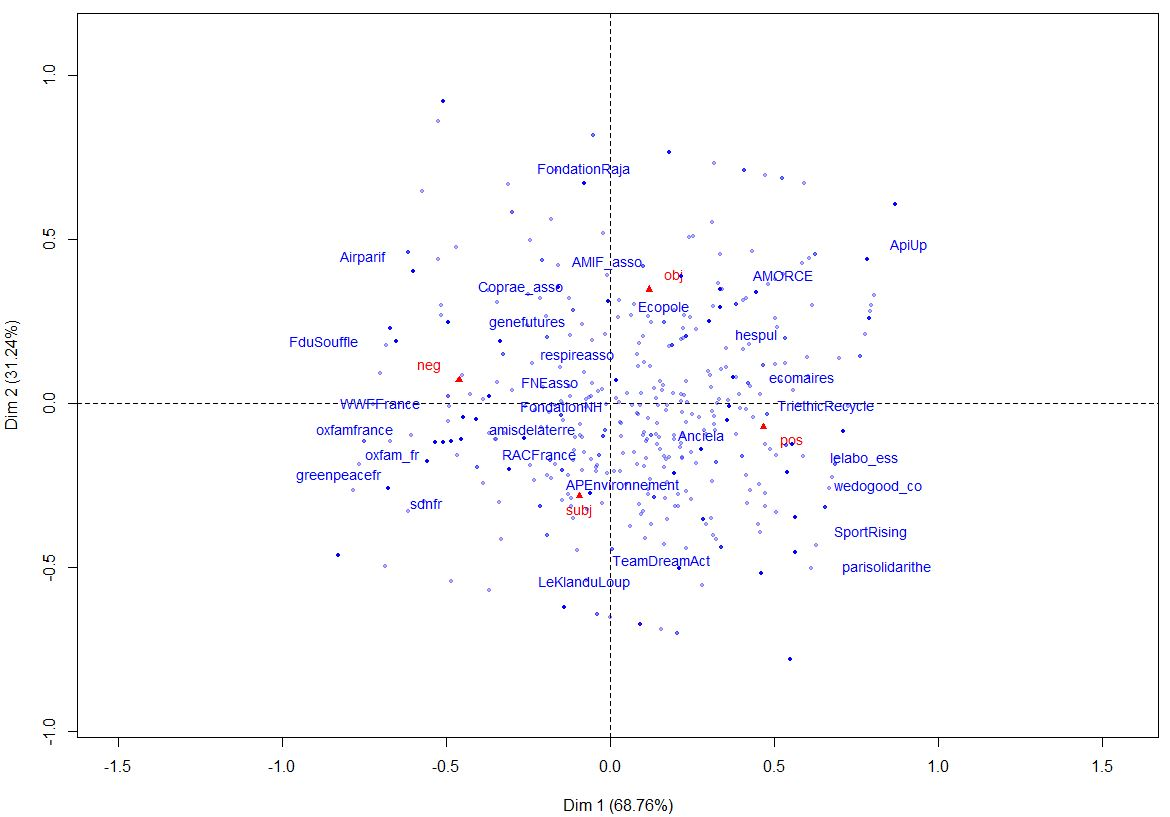
\includegraphics[width=\linewidth]{fig/AFC_entreprises.JPG}
            \end{figure}

            Tout en bas, Le Klan du Loup et TeamDreamAct sont caractéristiques d’un discours majoritairement subjectif, marqué par des interactions importantes avec les utilisateurs et par des prises de positions fortes, usant parfois d’humour, d’ironie ou de sarcasme.


            \begin{quotation}
                \citit{Les trois plaies pour la biodiversité : Chasse, pêche et agriculture \\
                https://t.co/AZ6Yv1iGYT \#biocentrisme \#environnement \#écologie} (Le Klan du Loup, Août 2016) \\
                \citit{"Malgré les intempéries... l'été approche alors ayez la fraîcheur écolo :) https://t.co/YzeQz41UFB https://t.co/vvORveDhqF"} (TeamDreamAct, juin 2016)
            \end{quotation}

            Le cadran inférieur droit correspond aux entreprises adoptant un discours plutôt subjectif mais positif. C’est le cas de parissolidarithe (association membre du \mouves), SportRising (coopérative sous forme de SCOP) ou encore wedogood (entreprise sociale).

            \begin{quotation}
               \citit{Quand le sport se met au service des hommes et de l'environnement! \@LaurentOlmo \@bbarbusse \@DominiqueCrochu  https://t.co/9Rtx40AGDJ} (SportRisin, septembre 2015) \\
                \citit{\@Green\_spector : bravo, toujours au top pour l'efficacité énergétique ! \#greenIT \#transition \#numérique} (wedogood\_co, décembre 2016)

            \end{quotation}



            Enfin, un discours positif et plutôt objectif est adopté par les organisations présentes dans le cadran supérieur droit, comme Amorce, réseau d'information et d'accompagnement en matière d'écologie, ou API'UP, association de récupération et recyclage des déchets.

            \begin{quotation}
               \citit{.\@AMORCE 1 million d'euros d'économie dans les collèges isérois grâce à la lutte contre le \#gapillagealimentaire \#BIO2016} (Amorce, mai 2016) \\
            \end{quotation}

            Dans l'étape suivante, nous proposons une approche plus fine, basée sur la correspondance entre le discours des organisations et des cadres rhétoriques prédéfinis.


        \subsubsection{Étude du cadrage du discours}

            362 hashtags utilisés au moins 15 fois dans le corpus ont été analysés pour être affectés aux huit cadres identifiés par \textcite{nisbet2009communicating}. 111 n’ont pu être affectés à aucun cadre rhétorique. Le tableau \ref{table:21hashtagsnisbet} détaille l’affectation des 251 hashtags qui correspondent à un cadre particulier.\\

            \begin{table}
                \caption{Affectation des hashtags aux registres}
                \label{table:21hashtagsnisbet}
                \footnotesize

                \begin{tabularx}{\linewidth}{|K{0.20\linewidth}|X|}
                \hline

                \textbf{Cadres}	&\textbf{Hashtags}
                \\ \hline

                Conflict and strategy	& enercoop, edf, ouiauxloups, projectrescueocean, antigaspi, confenvi, plantfortheplanet, nddl, legranddebat, colloque, fessenheim, conférence, cashinvestigation, stopcharbon, bure, afp, stoppesticides, macron, lemissionpolitique, congrèsamorce, monsanto, trump, 15minutespourconvaincre, zerodeforestation\\ \hline
                Economic development and competitiveness & 	dd, emploi, innovation, developpementdurable, développementdurable, crowdfunding, startup, économie, développement, entreprise, entreprises, numérique, devdurable, appelaprojets, agroforesterie, emplois, financement, bioéconomie, planification, bâtiment, finance, fiscalité, greentech, travail, economie, agriculteurs, banques, developpement, économique, btp\\ \hline
                Middle way/alternative path	& bio, recyclage, economiecirculaire, durable, zerowaste, transitionenergetique, économiecirculaire, zerodechet, transition, agroécologie, upcycling, transitionénergétique, zérodéchet, photovoltaïque, tri, agroecologie, renouvelable, éolien, circuitscourts, réemploi, circuitcourt, biodéchets, photovoltaique, renouvelables, permaculture, local, transitionecologique, recycler, territoires, biocentrisme, solaire, vélo, biogaz, nuitagroecologie, compostage, alternatives, rénovation, économiesénergie, autoconsommation, diy, palmedurable, mondevivable, collecte, palmedurable, jesuisecoloquand, ecoconception, aménagement, changement, écoquartier, territoire, valorisation, compost, circulaire, smartcity, energiesrenouvelables, vegan, circulareconomy\\ \hline
                Morality and ethics	& rse, responsable, solidaire, solidarité, greenwashing, prévention, ecoresponsable, equitable, chasse, sociale, inégalités, congésolidaire, écoresponsable, solidaires, équitable, fairfinance, commerceequitable, don, engagement, solidarite\\ \hline
                Pandora’s box	& déchets, pollution, dechets, déchet, gaspillage, déforestation, pollutiondelair, obsolescence, deforestation, pollutionair, fukushima, gaspillagealimentaire, cancer, waste, obsolescenceprogrammée, victimes, obsolescenceprogrammee, airpollution, perturbateursendocriniens\\ \hline
                Public accountability and governance &	cop21, ess, energiecitoyenne, cop22, loibiodiv, legislatives2017, socent, scop, accorddeparis, ceta, collectivités, associations, association, citoyen, ecophyto, scic, cop20, ue, loi1901, coop, citoyenne, g7, coopérative, presidentielle2017, loi, tafta, coopératives, servicecivique, citoyenneté, asso\\ \hline
                Scientific and technical uncertainty &	climat, énergie, pesticides, biodiversité, nucléaire, charbon, énergétique, energie, climatechange, huiledepalme, air, eau, biodiversite, énergies, changementclimatique, nucleaire, climatique, climateinitiative, emballages, électricité, ogm, pêcheprofonde, pétrole, gazdeschiste, oceanclimax, nucléaires, papier, climatdatalab, glyphosate, plastique, nanoparticules, gaz, co2, méthanisation, pesticide, epr, réchauffementclimatique, qualitéair, océan, rechauffementclimatique, plastiques, ges, réchauffement, abeilles, néonicotinoïdes, qualiteair, réseauxdechaleur\\ \hline
                Social Progress	& agriculture, santé, sport, alimentation, insertion, consommation, social, habitat, genderday, éducation, mobilité, urbanisme, transport, précarité, sante, logement, education, transports, humanitaire, construction, formation, mobilite, alimentaire, pauvreté\\ \hline


                \end{tabularx}
            \end{table}

            On détermine ainsi, pour chaque utilisateur, le nombre de tweets correspondant à chacun des cadres rhétoriques. Ceci prend la forme d’une table de contingence qui donne lieu à une analyse factorielle des correspondances (AFC). \\

            La variable « catégorie d’organisation » ayant 7 modalités, l’AFC répartit la variance sur 6 dimensions. Les deux premières dimensions expliquent à elles seules 88.8\% de la variance (encadré \ref{encadre:6afcsummary}), ce qui est tout à fait suffisant pour l’analyse. La seule première dimension factorielle correspond à 58.6\% de variance. La figure \ref{figure:7AFC} représente la projection des variables sur les deux premières dimensions. L’interprétation de cette carte factorielle est complétée par les données présentées dans l’encadré \ref{encadre:6afcsummary}, qui détaille la contribution de chaque modalité à la contribution des deux axes (ctr), ainsi que sa qualité de projection (cos2). \\


            \begin{encadre}
                \caption{Synthèse de l’AFC}
                \label{encadre:6afcsummary}
                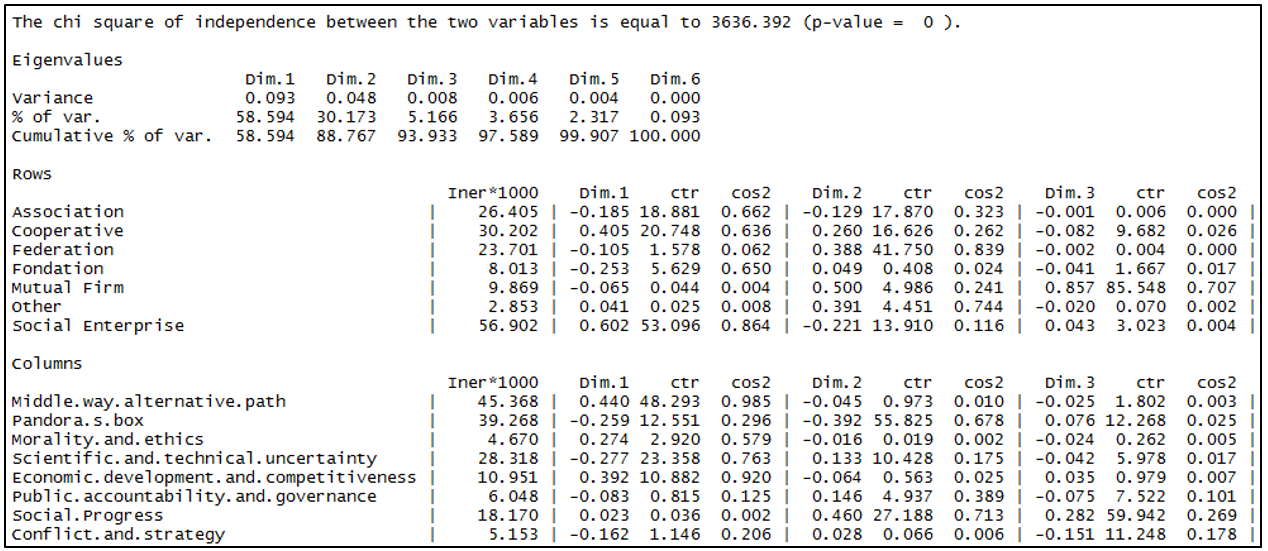
\includegraphics[width = \textwidth]{fig/fig6.png}
            \end{encadre}


            \textbf{La première dimension} est la plus importante et explique 58 \% de la variance. Elle oppose les coopératives et entreprises sociales (coordonnées positives) aux associations et fondations (coordonnées négatives). Les premières mobilisent particulièrement les registres du développement économique / compétitivité et des alternatives / compromis. Les secondes ont davantage recours au registre de l’incertitude scientifique et technologique, et de manière un peu moins nette à celui de la boîte de Pandore et celui des conflits et stratégie. L’axe horizontal oppose ainsi des organisations qui lient le discours environnemental avec une recherche d’opportunités d’innovation et de développement économique, à des organisations qui s’intéressent à l’état scientifique des choses, c’est-à-dire à l’avancement des connaissances relatives à l’écologie. Le secteur non lucratif (associations et fondations) semble aussi plus pessimiste et plus prompt à mettre en avant le danger que fait peser la situation environnementale et à ouvrir un débat critique sur ces questions. \\

            \begin{landscape}
            \begin{figure}
                \caption{Correspondance entre organisations et registres : carte factorielle}
                \label{figure:7AFC}
                \centering
                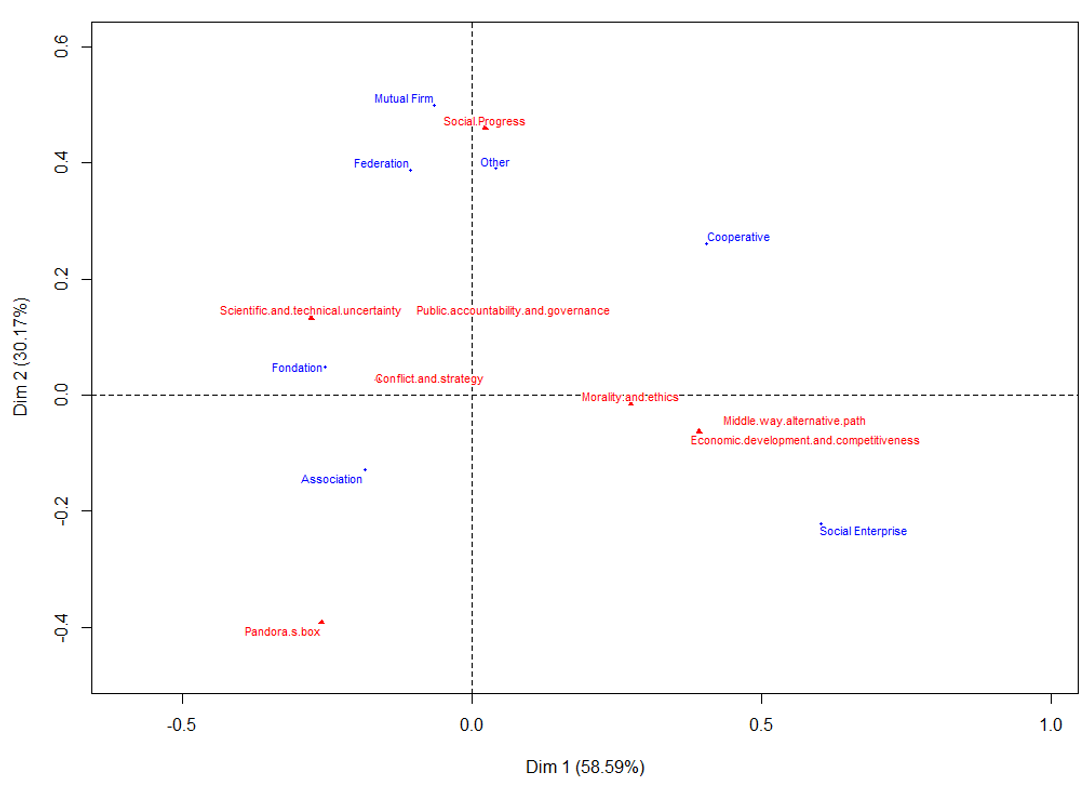
\includegraphics[height = 0.90\textheight]{fig/fig7.png}
            \end{figure}
            \end{landscape}


            \textbf{La seconde dimension factorielle} correspond à 30 \% de la variance totale. Elle met en évidence une correspondance significative entre les mutuelles et fédérations ainsi que la catégorie « autre » (c’est-à-dire les incubateurs et comptes Twitter de marques ou d’évènements) et le cadre du Progrès Social. Le cadre de la Responsabilité publique et de la gouvernance est aussi nettement associé à ces organisations. Il est intéressant d’observer que les coopératives, bien que moins fortement associées à ces cadres, les utilisent davantage que les entreprises sociales et, de façon assez surprenante, que les associations.

            La proximité avec le cadre du Progrès Social s’explique notamment par la mission première des mutuelles qui opère dans le secteur de la santé et de la protection sociale. Elles plébiscitent donc les hashtags relatifs à ce cadre. La même explication peut s’appliquer à la catégorie Fédérations, qui intègre un grand nombre de fédérations mutualistes. Le discours environnemental de ces organisations est donc fortement lié aux questions sociales et sociétales. \\

            Le cadre de la Responsabilité publique et de la gouvernance renvoie à la fois à des questions de politiques publiques et à la gouvernance des entreprises. Or, l’ESS est marquée par des modes de gouvernance particuliers, reposant sur une logique participative et démocratique. Ceci est particulièrement vrai dans les mutuelles qui appartiennent à leurs clients, et dans les coopératives qui peuvent être détenues par différents groupes de parties prenantes. \\

            A l’inverse, associations et entreprises sociales sont ici plus fortement associées avec le cadre de la Boite de Pandore. Ceci ne signifie pas que les associations ne se préoccupent pas de progrès social ou de gouvernance, mais que ces cadres ne sont pas utilisés conjointement au discours environnemental. Comme observé pour la première dimension, les associations utilisent plutôt un cadre « dramatique » pour promouvoir la transition écologique.  \\

            \textbf{La troisième dimension factorielle} n’est pas représentée sur la figure \ref{figure:7AFC}, mais elle présente une meilleure qualité de projection des mutuelles qui confirme la correspondance avec le cadre du Progrès Social (encadré \ref{encadre:6afcsummary}).




    \subsection{Etude de la performance des tweets }

        \subsubsection{Selon le cadrage rhétorique}

            L’AFC montre que les différentes formes organisationnelles de l’ESS ont recours à des cadres rhétoriques différents pour porter le discours environnemental. Ceci conduit à se demander lesquels sont les plus efficaces pour permettre la diffusion des idées véhiculées dans les tweets. Pour mesurer cette performance, deux indicateurs sont utilisés : le nombre de retweets et le nombre de favoris. Pour chaque cadre rhétorique, le tableau \ref{table:22rtmean} indique le nombre moyen de retweets et de mise en favoris des tweets.

            \begin{table}
                \caption{Nombre moyen de retweets et de favoris en fonction du cadre rhétorique}
                \label{table:22rtmean}
                \centering
                \small
                \begin{tabularx}{\textwidth}{|X|R|R|}
                    \hline
                    \head{Cadre rhétorique}&	\head{Nombre de retweets}&	\finalhead{Nombre de favoris} \\ \hline

                    Conflict and strategy&	16.10	&10.88 \\ \hline
                    Scientific and technical uncertainty&	8.83&	5.09\\ \hline
                    Public accountability and governance&	6.70&	4.10\\ \hline
                    Pandora’s box&	4.69&	2.25\\ \hline
                    Morality and ethics	&3.54&	2.26\\ \hline
                    Middle way/alternative path&	3.18&	2.86\\ \hline
                    Social Progress	&2.97&	2.24\\ \hline
                    Economic development and competitiveness&	2.29&	1.95\\ \hline

                \end{tabularx}
            \end{table}


            Le cadre « Conflit et stratégie » semble nettement plus performant que les autres, avec plus du double de retweets par rapport au second registre (Incertitude scientifique et technique). Les cadres « Incertitude scientifique et technique » et « Responsabilité publique et gouvernance » sont également performants. Ils correspondent, pour le premier, aux hashtags renvoyant au niveau actuel de la connaissance sur les questions d’écologie, et pour le second, aux questions de décisions publiques et de responsabilité des gouvernements, des entreprises et des individus.

            Bien que les tweets recourant au cadre de la « Boite de Pandore » soient moins retweetés, ils sont toutefois plus performants que les tweets concernant la morale, les alternatives, le progrès social ou le développement économique.  \\

            Une limite à cette lecture statistique est que ces deux variables font ressortir un certain nombre de valeurs extrêmes, c’est-à-dire des tweets qui ont été massivement partagés ou mis en favoris et qui viennent gonfler la moyenne. Or, il n’est pas pertinent d’éliminer ces outliers, car c’est précisément cet « effet buzz » qui est recherché sur les réseaux sociaux afin de diffuser le plus efficacement un contenu. On cherche au contraire à déterminer dans quel cadre rhétorique s’inscrivent les tweets qui ont bénéficié de cet effet. Pour cela, le tableau \ref{table:23toptweets} présente les 20 tweets ayant été le plus retweetés sur le réseau social. Il s’agit essentiellement de tweets très engagés et critiques, utilisant des mécanismes rhétoriques comme l’ironie ou le sarcasme. Ils s’inscrivent dans une logique d’interpellation en mentionnant ou en s’adressant directement à des responsables politiques. Les tweets peuvent aussi s’adresser à des grandes entreprises, mises en cause pour leur comportement vis-à-vis de l’environnement. L’urgence d’agir est aussi mise en avant dans ces tweets, ainsi que le danger engendré par certaines pratiques, notamment en lien avec l’industrie nucléaire. \\


            \begin{landscape}
                \begin{table}
                \caption{Tweets les plus partagés}
                \label{table:23toptweets}
                    \centering
                    \scriptsize
                    \begin{tabularx}{\linewidth}{|L|K{0.8\linewidth}|R|}
                    \hline
                    \head{Auteur}	&	\head{texte}	&	\finalhead{Nombre de retweets}	\\ \hline

                        FondationNH	&	\#Trump : Sortir de l'Accord de Paris c'est un contre-sens tragique de l'histoire!  \#climat https://t.co/XONkeg3fJH	&	1012	\\ \hline
                        oxfamfrance	&	RT cette photo pour rappeler à @fhollande ses engagements sur le \#climat. \#LikeTaPlanete http://t.co/NMmnXPy5M5	&	1000	\\ \hline
                        greenpeacefr	&	Environnement: le programme \#Macron est incohérent et ne remet pas en cause le système actuel désastreux \#TelSonne https://t.co/iJgbPWaeCa	&	829	\\ \hline
                        FondationNH	&	Donald Trump réalise un acte stupide et criminel qui va à rebours du sens de l’Histoire en sortant de l' \#AccorddeParis  \#Trump \#climat	&	501	\\ \hline
                        WWFFrance	&	Malgré une sortie possible de l’\#AccordDeParis, les villes vont intensifier leur action pour le \#climat aux États-U… https://t.co/3WMhAKmf04	&	495	\\ \hline
                        WWFFrance	&	En cette journée mondiale de l'\#environnement, rendons hommage aux poumons de notre planète : les forêts ! ️… https://t.co/Gbg2vh2oWD	&	491	\\ \hline
                        greenpeacefr	&	Impunité des grands pollueurs, drames écologiques en pagaille...et il faudrait se taire ? \#NosVoixSontEssentielles… https://t.co/lv0jSPeJfp	&	338	\\ \hline
                        greenpeacefr	&	Non, le charbon n’a pas remplacé le \#nucléaire en Allemagne. Mensonge @EmmanuelMacron \#AlterQG \#LEmissionpolitique https://t.co/A9Hq7sZD3D	&	328	\\ \hline
                        greenpeacefr	&	\#Fukushima : la France n’a pas tiré les leçons des accidents \#nucléaires. Le danger plus présent que jamais du côté… https://t.co/croQ1NiRbb	&	286	\\ \hline
                        greenpeacefr	&	Pendant que la France s'enfonce dans sa fuite en avant \#nucléaire, les Suisses lui tournent le dos. https://t.co/KXTtk8uGnM via @libe	&	279	\\ \hline
                        RACFrance	&	\#PLF2017: la France doit respecter ses engagements! Augmentez les recettes de la \#TTF pr le développement \& \#climat… https://t.co/RwBNDSbB89	&	275	\\ \hline
                        greenpeacefr	&	Pas un mot d'@EmmanuelMacron sur l'écologie. Étonnant? Pas tant. \#alterQG \#15minutesPourConvaincre https://t.co/iJgbPWaeCa	&	262	\\ \hline
                        greenpeacefr	&	[BREAKING] Scandale anomalies Creusot: des documents prouvent qu' EDF et AREVA étaient alertées dès 2005 \#nucléaire https://t.co/sbAU6D7H1T	&	242	\\ \hline
                        FondationNH	&	\#LoiBiodiv : Le Sénat préfère les pesticides aux abeilles! https://t.co/gC8wrfjNhp  \#neonicotinoides \#biodiversite https://t.co/x8BPdS0jcq	&	227	\\ \hline
                        amisdelaterre	&	Ils reviennent les \#Pinocchio2015 \#climat \& n'échapperont pas à vos votes! A vous de jouer https://t.co/yZCNHJwUYX \newline https://t.co/JRUGW1fT8U	&	225	\\ \hline
                        FondationNH	&	Contre les faits,contre la science, le Sénat refuse d'interdire pesticides \#néonicotinoïdes \#LoiBiodiv \#biodiversité https://t.co/kBeHDB8rrb	&	200	\\ \hline
                        attac\_fr &	Transition sociale et écologique = 0 \newline Lutte contre l'impunité fiscale = 0 \newline \#2017LeDebat	&	190	\\ \hline
                        greenpeacefr	&	La faillite du \#nucléaire, de moins en moins discrète : \#EDF admet un risque de black-out. https://t.co/tnk5uIdSIu https://t.co/Xs86WaTERF	&	187	\\ \hline
                        FNEasso	&	\#NDDL : qui va payer la destruction de l'environnement et la construction d'infrastructures inutiles ? https://t.co/2YKZbNFcj6	&	183	\\ \hline
                        amisdelaterre	&	.@SocieteGenerale \& @BNPParibas soutiennent \#gazdeschiste aux USA. Elles ne peuvent pas le faire ici!… https://t.co/6e0j2ccF6Y	&	178	\\ \hline
                    \end{tabularx}

                \end{table}
            \end{landscape}



            Une bonne performance d’un tweet, soit une bonne visibilité sur le réseau, semble ainsi résulter d’un propos vivement engagé, voire impertinent, appelant à la controverse et au débat et s’appuyant sur l’actualité. Twitter apparaît donc ici comme un réseau social favorisant la polémique, le débat et la prise de position. Le meilleur moyen de promouvoir la transition écologique sur ce réseau est donc d’adopter une posture engagée, quitte à recourir à l’exagération et à prendre à partie les opposants aux idées défendues. Ce sont donc les stratégies de communication adoptées par les organisations à but non lucratif qui semblent les plus efficaces sur Twitter. La communication des coopératives et entreprises sociales, reposant sur des aspects économiques et sur la présentation d’alternatives innovantes, ou celle des mutuelles, basée sur le progrès social, semblent beaucoup moins performantes.  \\

            Cependant, les tweets les plus partagés sont diffusés par des entreprises de l’ESS très connues du grand public et ayant un grand nombre d’abonnés. Or, il a été démontré que le nombre d’abonnés a une forte influence sur la performance d'un tweet. On peut dès lors se demander si les tweets sont performants en raison des cadres rhétoriques qu’ils utilisent, ou bien parce qu’ils sont publiés par des organisations ayant un grand nombre d’abonnés, qui sont aussi plus susceptibles d’utiliser ces cadres. Les organisations ayant le plus grand nombre de tweets (comme la Fondation Nicolas Hulot, GreenPeace, WWF ou Attac) sont en effet connues pour leur engagement militant et leurs prises de positions politiques en faveur de l’écologie. Pour éliminer l’impact de la popularité de l’émetteur, c’est-à-dire de son nombre d’abonnés, on utilise le niveau d'engagement, qui a été défini de la manière suivante (\ref{twitter:perf}) : \\
            \begin{center}
                $Engagement = \dfrac{Nombre\ de\ retweets + Nombre\ de \ favoris}{Nombre\ d'abonnés} \times 1000$ \\
            \end{center}

            La valeur moyenne de cet indicateur est calculée pour chaque cadre rhétorique. Les résultats sont présentés dans le tableau \ref{table:23perfmean}. Le test de Mann-Whitney est utilisé pour déterminer si ces écarts sont significatifs (tableau \ref{table:24MW})\footnote{Ce test non paramétrique nécessite des échantillons de même taille : aussi, une sélection aléatoire de 800 tweets de chaque cadre est effectuée préalablement au test} . Comme précédemment, on applique la correction de Bonferoni (le niveau de significativité est interprété selon la p-value divisée par 28).

            \begin{table}
                \caption{Performance des tweets en fonction du cadre rhétorique}
                \label{table:23perfmean}
                \centering
                \small
                \begin{tabularx}{\textwidth}{|K{0.5\textwidth}|R|}
                    \hline
                    \head{Cadre rhétorique}&	\finalhead{Engagement} \\ \hline

                    Conflict and strategy&	2.59\\ \hline
                    Middle way/alternative path	&2.55\\ \hline
                    Social Progress&	2.07\\ \hline
                    Morality and ethics&2.02\\ \hline
                    Economic development and competitiveness&	2.02\\ \hline
                    Public accountability and governance&	1.89\\ \hline
                    Scientific and technical uncertainty&	1.55\\ \hline
                    Pandora’s box&	1.43\\ \hline


                \end{tabularx}
            \end{table}


            \begin{table}
                \caption{Comparaison de la performance des cadres - test de Mann-Whitney}
                \label{table:24MW}
                \centering
                \scriptsize
                \begin{tabularx}{\linewidth}{|K{2cm}|K{0.3cm}|L|L|L|L|L|L|L|L|}
                \hline
                &&Middle way,  alt. path &	Pandora’s box &	Morality and ethics &	Sci. and tech. uncertainty	& Economic dev. and comp. &	Public account. and gov. &	Social Progress &	Conflict and strategy\\ \hline

                \multirow{2}{=}{Middle way, alt. path}	&	U	&	338106	&	292044***	&	323043	&	309554**	&	305352***	&	267150***	&	295958***	&	333182	\\
                &		p	&	(0.3212)	&	(0.0000)	&	(0.0081)	&	(0.0001)	&	(0.0000)	&	(0.0000)	&	(0.0000)	&	(0.1573)	\\ \hline
                \multirow{2}{=}{Pandora’s box}	&	U	&	291902***	&	331794	&	324866	&	336008	&	326230	&	324744	&	335613	&	299068***	\\
                &		p	&	(0.0000)	&	(0.1192)	&	(0.0178)	&	(0.2446)	&	(0.0218)	&	(0.0236)	&	(0.1925)	&	(0.0000)	\\ \hline
                \multirow{2}{=}{Morality and ethics}	&	U	&	313373*	&	330962	&	341964	&	339855	&	339681	&	326124	&	331795	&	312443*	\\
                &		p	&	(0.0002)	&	(0.0830)	&	(0.5000)	&	(0.4003)	&	(0.3793)	&	(0.0245)	&	(0.0676)	&	(0.0003)	\\ \hline
                \multirow{2}{=}{Sci. and tech. uncertainty}	&	U	&	305983***	&	336454	&	334854	&	337970	&	322920	&	305533***	&	338640	&	309926*	\\
                &		p	&	(0.0000)	&	(0.2672)	&	(0.1964)	&	(0.3260)	&	(0.0096)	&	(0.0000)	&	(0.3410)	&	(0.0002)	\\ \hline
                \multirow{2}{=}{Economic dev. and comp.}	&	U	&	322675	&	341874	&	337290	&	334633	&	340986	&	310761**	&	333553	&	315211	\\
                &		p	&	(0.0095)	&	(0.4957)	&	(0.2695)	&	(0.1960)	&	(0.4504)	&	(0.0000)	&	(0.1112)	&	(0.0009)	\\ \hline
                \multirow{2}{=}{Public account. / gov.}	&	U	&	263358***	&	320946	&	322155	&	329282	&	309356***	&	330485	&	328110	&	296710***	\\
                &		p	&	(0.0000)	&	(0.0053)	&	(0.0064)	&	(0.0689)	&	(0.0000)	&	(0.0861)	&	(0.0283)	&	(0.0000)	\\ \hline
                \multirow{2}{=}{Social Progress}	&	U	&	306896***	&	336084	&	329490	&	331729	&	335453	&	330092	&	339978	&	299813***	\\
                &		p	&	(0.0000)	&	(0.2205)	&	(0.0373)	&	(0.0959)	&	(0.1739)	&	(0.0562)	&	(0.3609)	&	(0.0000)	\\ \hline
                \multirow{2}{=}{Conflict and strategy}	&	U	&	336426	&	304477***	&	310647**	&	291900***	&	320314	&	285108***	&	299272***	&	336144	\\
                &		p	&	(0.2699)	&	(0.0000)	&	(0.0001)	&	(0.0000)	&	(0.0057)	&	(0.0000)	&	(0.0000)	&	(0.2643)	\\ \hline


                \end{tabularx}
            \end{table}


            L’impact du nombre d’abonnés étant éliminé, le cadre « Conflits et stratégie » apparaît toujours comme le plus performant, mais cette fois-ci au même niveau que le cadre des « Compromis et alternatives ». La faible performance de ce dernier cadre dans la précédente analyse vient donc du fait qu’il est plutôt mobilisé par des organisations ayant peu d’abonnés. A nombre d’abonnés égal, ce cadre est donc efficace pour favoriser la diffusion des tweets. Il en va de même pour les cadres du « Progrès social », de la « Moralité et l’éthique » et du « Développement économique et compétitivité. Toutefois, à l’exception des deux cadres les plus performants, les résultats ne montrent pas de différence significative entre les cadres rhétoriques.



         \subsubsection{Selon le sentiment et l'objectivité}
            De la même manière que l'on a étudié la performance des registres rhétoriques utilisés, on peut comparer les performances selon l'usage de tweets positifs ou négatifs, et objectifs ou subjectifs. Les écarts sont présentés dans le tableau \ref{table:perftweet1}.

            Les résultats des tests de comparaison sont très significatifs (tableau \ref{table:perftweet2}), montrant ainsi que les écarts de performance ne sont pas liés à l'erreur d'échantillonage. Les tweets ayant un caractère négatif sont nettement plus retweetés et plus mis en favoris que les tweets positifs. Cependant, une fois éliminé l'effet du nombre d'abonnés, les tweets positifs obtiennent en réalité un taux d'engagement plus élevé. Ceci semble indiquer que si un discours négatif est plus souvent adopté par des organisations ayant un grand nombre d'abonnés, le recours à un discours positif est préférable pour atteindre son audience. Il en va de même avec les tweets objectifs qui obtiennent un meilleur taux d'engagement, bien que les organisations avec un grand nombre d'abonnés obtiennent un fort impact avec des tweets subjectifs.

            \begin{table}[]
            \caption{Performance des tweets selon le sentiment et l'objectivité}
            \label{table:perftweet1}
                \centering
                \small
                \begin{tabularx}{\linewidth}{|K{0.16\linewidth}|R|R|R|R|R|R|}
                    \hline
                    & \multicolumn{3}{|c|}{\textbf{Sentiment}} & \multicolumn{3}{|c|}{\textbf{Objectivité}} \\ \hline

                    & \head{Positif} & \head{Négatif} & \head{Ecart (\%)} & \head{Objectif} & \head{Subjectif} &  \finalhead{Ecart (\%)} \\ \hline

                    \textbf{Engagement} & 28.34 & 20.75 & 37 \% & 26.31 & 22.81 & 15 \% \\ \hline

                    \textbf{Nombre de retweets} & 5.23 & 10.88 & 108 \% & 6.63 & 9.61 & 45 \% \\ \hline

                    \textbf{Nombre de favoris} & 4.66 & 7.81 & 68 \% & 5.01 & 7.21 & 44 \% \\ \hline
                \end{tabularx}
            \end{table}

            \begin{table}[]
            \caption{Performance des tweets selon le sentiment et l'objectivité - tests statistiques}
            \label{table:perftweet2}
                \centering
                \small
                \begin{tabularx}{\linewidth}{
                    |K{0.14\linewidth}
                    |K{0.10\linewidth}
                    |L
                    |L
                    |L
                |}
                    \hline
                    & \head{Test} & \head{Engagement} & \head{Nombre de retweets} & \finalhead{Nombre de favoris} \\ \hline
                    \multirow{4}{*}{Objectivité}
                        & \multirow{2}{*}{Test T}
                            & $T = 8.4829$*** & $T = -13.1571$*** & $T = -10.7853$*** \\
                            & & $p = .000$ & $p = .000$ & $p = .000$ \\ \cline{2-5}
                        & \multirow{2}{*}{Wilcoxon}
                            & $W = 13284236$*** & $W = 7004314$*** & $W = 4775770$*** \\
                            & & $p = .000$ & $p = .000$ & $p = .000$ \\ \hline

                    \multirow{4}{*}{Sentiment}
                        & \multirow{2}{*}{Test T}
                            & $T = 15.8020$*** & $ T = -27.3647$*** & $T = -17.7536$*** \\
                            & & $p = .000$ & $p = .000$ & $p = .000$ \\ \cline{2-5}
                        & \multirow{2}{*}{Wilcoxon}
                            & $W = 13593125$*** & $W = 5722547$*** & $W = 4925017$*** \\
                            & & $p = .000$ & $p = .000$ & $p = .000$ \\ \hline

                \end{tabularx}
            \end{table}




            % \todo[inline]{Pourquoi à la fois un test t et wilcoxon ? Vérifier normalité}

                    \section{Discussion}

    \subsection{Stratégies de communication}

        \subsubsection{Utilisation du réseau}
            %\todo[inline]{Rajouter la partie correspondante dans les résultats ou bien supprimer ce paragraphe}
           % Les résultats montrent une grande variété d’utilisation du réseau, ce qui confirme les observations de \textcite{guo2017speaking}. Twitter est particulièrement investi par Des associations et fondations qui s’adressent à un public très large qu’elles peuvent facilement atteindre sur Twitter. Ce sont les plus prolifiques en termes de nombre de tweets. Cependant, Twitter est principalement utilisé comme un média de diffusion d’informations plutôt que comme un moyen d’échange et d’interaction. Conformément à ce qui a été observé par \sources, la part des tweets consacrée à répondre à d’autres utilisateurs est faible. En revanche, les mentions, qui permettent d’interpeler, de référencer ou de citer un autre utilisateur, sont plus utilisées. Les organisations s’inscrivent donc bien dans une logique de réseau et d’interconnexion, mais la place pour l’échange et la discussion reste limitée. Ce constat est légèrement moins marqué pour les entreprises sociales qui consacrent une part un peu plus importante des tweets à répondre à d’autres utilisateurs (raison ?). Ces résultats rejoignent ceux de \textcite{guo2014tweeting}, qui observent trois modalités d’usage de Twitter. Il s’agit de diffuser de l’information, de créer une communauté et d’appeler l’audience à agir. Les résultats montrent que 68\% des tweets sont consacrés à diffuser une information alors que seulement 20\% visent à créer une communauté, et 12\% appellent à l’action. Une observation comparable est faite par \textcite{mariaux2017promouvoir} qui distinguent cette fois cinq catégories de tweets visant à promouvoir la transition écologique. Ils reposent sur une logique d’information, de mise en évidence d’alternatives, de dialogue, d’action ou de critique. A nouveau le registre prédominant est celui de l’information (35\%), qui rassemble des tweets à sens unique, qui n’attendent pas de réponse ou de réaction de l’audience. La catégorie de tweets visant à promouvoir des alternatives innovantes (20\%) regroupe aussi un contenu à sens unique. Les tweets consacrés à encourager un échange ente l’organisation et son audience représentent 20\% du volume. Cependant, une part importante de ce contenu invite à une rencontre en dehors du réseau, à l’occasion de forum, de conférences ou de portes ouvertes. Ils n’ouvrent pas réellement à une discussion au sein du réseau. \\

            Un enjeu important sur Twitter est la visibilité des contenus diffusés. Le réseau étant utilisé comme un outil d’information, son efficacité repose sur la capacité à atteindre une audience large. Dans le contexte du secteur non lucratif aux USA, \textcite{guo2017speaking} ont montré que le nombre d’abonnés et le nombre de tweets diffusés constituaient des facteurs fondamentaux pour atteindre l’audience la plus large possible. Les résultats de la présente étude, menée dans un contexte plus large, celui de l’ESS, confirment ces observations. Au-delà de la stratégie rhétorique, au-delà du type de contenus diffusés, ce sont le nombre d’abonnés et le volume des tweets qui permettent d’atteindre un public large. Or la popularité sur ce réseau est fortement liée à la popularité médiatique ou sociétale d’une personne ou d’une organisation. Une organisation qui bénéficie déjà d’une certaine renommée peut donc atteindre plus facilement une large audience sur Twitter. Ceci est confirmé par l’observation de notre échantillon pour lequel les organisations ayant le plus d’abonnés sont des associations et fondations connues du grand public. Au regard de la transition écologique, ces organisations jouent donc un rôle fondamental dans la diffusion des alternatives et dans la promotion de comportements et de modes de vie ou de production plus respectueux de l’environnement. Naturellement, toutes ces organisations n’ont pas vocation à promouvoir la cause environnementale. Des associations comme les Restos du Cœur, la Croix Rouge ou Oxfam France, qui ont toutes les trois plus de 100 000 abonnés sur Twitter, ont des missions orientées vers des problématiques sociales éloignées des préoccupations environnementales. Pourtant, elles ont, en raison de leur popularité, la capacité à porter et à promouvoir les questions d’écologie de façon plus efficace que des organisations moins connues dédiées à l’environnement. Dans une recherche publiée en 2014, \textcite{buchs2014role} montre que l’investissement dans une organisation environnementale conduit à modifier les comportement individuels vers des pratiques plus responsables. Cependant, elle souligne la portée limitée de ces seules organisations, et souhaite encourager les organisations du secteur non lucratif à porter la thématique de l’écologie, même si elle semble éloignée de leur mission première. La présente recherche conduit à soutenir ce propos : sur un réseau social comme Twitter, qui permet d’atteindre un public extrêmement large et divers, les entreprises de l’ESS bénéficiant d’une audience importante sont en capacité de promouvoir efficacement la transition écologique.   \\

            L’étude met également en évidence la façon dont les utilisateurs sont connectés sur le réseau social. Elle fait apparaître une forte interconnexion entre les organisations de l’ESS : bien que des communautés se distinguent, celles-ci sont le plus souvent très liées entre elles. Deux communautés font exception. Les coopératives agricoles forment un ensemble d’organisations très connectées entre elles, mais ayant peu de lien avec le reste de l’ESS. Elles s’identifient donc davantage par leur activité que par leur appartenance à l’ESS. Ceci peut s’expliquer par le fait que le choix du mode coopératif repose essentiellement sur les spécificités de leur activité : la production agricole et les conditions difficiles des agriculteurs en France imposent la mise en commun de certains moyens de production et de certains processus, afin de mieux résister à la concurrence internationale. Ces entreprises ne semblent pas identifier de proximité particulière avec l’ESS dans son ensemble, mais seulement avec les organisations qui partagent la même activité.
            De manière similaire, les mutuelles forment une communauté à part du reste de l’ESS. Les mutuelles ont un positionnement spécifique au sein de l’ESS, car elles sont exclusivement dédiées aux activités de l’assurance et de la santé. Elles montrent toutefois des liens plus forts avec le reste de l’ESS, notamment avec les associations professionnelles comme le CNCRES mais aussi avec des organisations du secteur caritatif donc les activités sont souvent proches et avec lesquelles des partenariats sont possibles.
            Une communauté regroupe les organisations dont la mission est liée avec l’environnement. Elle est toutefois très liée avec le reste de l’ESS, en particulier le mouvement caritatif, le mouvement des entreprises sociales et le mouvement coopératif. Ceci traduit le fait que la cause environnementale est prise en charge par différents types d’organisations et à travers différents statuts. Des associations et fondations vont se trouver plutôt dans une logique de protection, de réparation ou de sensibilisation (Green Peace, Fondation Nicolas Hulot…) quand des coopératives ou entreprises sociales vont chercher à développer des modes de production alternatifs et plus respectueux (Enercoop, Biocoop).\\

            Les six communautés identifiées (Entreprises agricoles, Mutuelles, Secteur caritatif, Action environnementale, Mouvement coopératif, Entrepreneuriat social) ne constituent pas une classification homogène qui permettrait d’aboutit à une typologie d’entreprises de l’ESS. Certains groupes sont regroupés autour d’un statut, d’autres selon une activité. Les interactions montrent que les organisations de l’ESS se rassemblent en fonction du statut, de l’activité mais aussi autour des organes fédérateurs de référence. L’ESS n’apparaît donc pas ici comme une économie segmentée, qui distinguerait nettement différentes catégories d’entreprises, mais plutôt comme une multiplicité de modèles économiques et d’activités interagissant entre elles.

        \subsubsection{Prise en compte de l’environnement}

            Il est intéressant de constater que les entreprises de l’ESS ayant adopté une logique de marché sont celles qui semblent avoir le mieux intégré le discours environnemental (coopératives, entreprises sociales). Ces entreprises, bien qu’elles intègrent les principes de l’ESS, s’appuient plus volontiers sur des pratiques commerciales et managériales du secteur lucratif. Ceci peut s’expliquer par des attentes plus fortes vis-à-vis de ces entreprises que pour le reste de l’ESS.  Comme le soulignent \textcite{dart2010green}, le secteur non lucratif bénéficie d’une image éthique et responsable qui minimise les attentes en matière de responsabilité sociale et environnementale. Déjà légitimées par leur action sociale, les organisations de ce secteur n’auraient plus besoin de justifier de leur responsabilité. Il est probable que les entreprises sociales et coopératives, en raison de la dimension commerciale de leur activité, ne bénéficient pas (ou pas autant) de cette légitimité a priori, et soient donc obligées de démontrer qu’elles s’inscrivent également dans une démarche éthique et responsable. En outre, en lien avec le développement de l’entrepreneuriat social, de nouveaux modes de financement dédiés à ce secteur apparaissent. Reconnaissant les principes de l’ESS, les investisseurs attendent un retour sur investissement beaucoup plus faible que pour des entreprises capitalistes. Cependant, les exigences en termes de performance sociale et environnementale sont élevées et les entreprises doivent démontrer leur contribution à la société, à travers des éléments concrets et des outils de mesure. Il est donc vraisemblable que les entreprises sociales passées par les circuits entrepreneuriaux dédiés à l’ESS (incubateurs, concours pour obtenir des aides, demandes de financements à des « Business Angels ») sont sensibles à toutes les facettes qui contribuent à créer de la valeur sociale, y compris au volet environnemental. Pour autant, il convient de s’interroger ici sur le lien entre la communication environnementale et la mise en œuvre d’actions concrètes. L’étude s’arrête à constater une différence dans le discours sur Twitter, c’est-à-dire dans la communication. Or, pour les raisons citées précédemment, les organisations de type entreprises sociales sont mieux au fait de la nécessité de valoriser leur impact et leur responsabilité environnementale. Les dernières années ont vu émerger des « startups sociales » portées par des entrepreneurs jeunes, issus de grandes écoles, très au fait de l’importance du marketing et de la communication et maitrisant très bien le fonctionnement des réseaux sociaux. On peut donc craindre que les résultats ne soient influencés par un « effet de communication » là où d’autres structures de l’ESS se concentreront sur leur activité et valorisent peut-être moins l’aspect environnemental dans leur discours. Ainsi, les organisations qui cherchent précisément à se différencier des entreprises de marché auront plus de peine à s’inscrire dans une forme de « culture de la communication ».  \\

            L’étude permet d’identifier plusieurs stratégies rhétoriques dans la promotion des thématiques environnementales. Deux stratégies s’opposent très nettement entre les organisations du secteur non lucratif et les organisations adoptant un positionnement proche des entreprises de marché. Ces dernières, à savoir les coopératives et entreprises sociales, communiquent à travers les cadres de l’innovation, de la mise en évidence d’alternatives et du développement économique. Pour elles, la transition écologique et le développement durable constituent une opportunité de développement, conformément à ce que propose \textcite{cretieneau2010economie}. Pour les associations et fondations, le discours repose sur la controverse, le débat d’idées et une prise de position militante. Elles peuvent avoir recours à un certain catastrophisme visant à alerter sur l’urgence du changement. Elles ont donc davantage un rôle de sensibilisation et d’information. Les mutuelles apparaissent un peu en marge de cette opposition. Pour elle, le discours environnemental est employé en lien avec leurs thématiques clés, à savoir le progrès social. L’environnement peut par exemple être abordé à travers son impact sur la santé et sur les bonnes pratiques à adopter. \\

            La stratégie adoptée par le secteur non lucratif, c’est-à-dire un discours engagé, militant, semble plus performant. Ces tweets souvent percutants sont largement partagés sur le réseau social. Pour autant, il n’est pas nécessairement pertinent pour toutes les organisations de l’adopter. Il correspond en effet à l’identité de certaines associations et fondations, dont la mission est d’interpeller, de critiquer et de militer. Cependant, pour des organisations s’inscrivant dans une logique commerciale, visant à se doter d’une identité « professionnelle » \parencite{dart2004being}, cette stratégie pourrait être contreproductive et conduire à délégitimer l’entreprise au regard de parties prenantes importantes pour elles (notamment les financeurs publics ou privés). C’est pourquoi elle est plutôt adoptée par des organisations comme Green Peace, qui revendique une totale indépendance et ne se finance qu’à travers des dons de particuliers. Les entreprises proches d’un fonctionnement de marché adoptent plutôt une stratégie politiquement plus neutre, s’appuyant sur leur dimension novatrice, économiquement performante, pour porter le discours environnemental. Elles courent ainsi le risque de passer à côté d’un « effet buzz », mais maintiennent une image innovante et constructive. Il faut toutefois souligner que si le cadre rhétorique des conflits et du débat obtient les meilleures performances, il n’est pas majoritaire, y compris au sein du secteur non lucratif. S’il est très utilisé par certaines organisations symboliques, \textcite{mariaux2017promouvoir} montent qu’une majorité de tweets adoptent plutôt un caractère factuel, s’appuyant sur des faits documentés plutôt que sur des opinions ou des prises de position. \\

            Enfin, l’impact des stratégies rhétoriques doit être relativisé. Le nombre d’abonnés d’une entreprise, c’est-à-dire sa popularité sur le réseau, semble plus important que le type de discours employé pour atteindre une large audience. Autrement dit, la portée du tweet dépend moins du contenu que de l’émetteur. Ceci étant, un statut provocateur, engagé, peut bénéficier de l’effet « buzz » et permettre in fine une augmentation du nombre d’abonnés. Ceci conduit à s’interroger sur le lien entre le contenu et le nombre d’abonnés : la popularité résulte-t-elle plutôt de la renommée de l’organisation en dehors du réseau, ou bien du type de contenus diffusés qui ont permis de susciter l’intérêt d’un grand nombre d’utilisateurs ? Les deux effets sont probablement combinés, dans la mesure où \textcite{guo2017speaking} ont également démontré l’importance du nombre de tweets sur la diffusion des contenus, ce que confirment nos résultats. On peut également s’interroger sur l’audience que l’on souhaite atteindre. Certains publics favorisent probablement des contenus engagés et sont plus intéressés par une prise de position vis-à-vis de l’actualité, quand d’autres recherchent sur Twitter une information plus neutre et moins subjective.


    \subsection{Contribution technique et méthodologique}

        Cette étude adopte des techniques récentes, encore peu utilisées dans les sciences humaines. Par son caractère original, elle vise à proposer ou développer des outils permettant à la science de gestion de profiter de l'essor des données disponibles sur internet.  Ce travail s'appuie sur plusieurs méthodes qui présentent chacune des intérêts pour la recherche, mais soulèvent aussi certains biais. \\

        L'utilisation d'un langage de programmation pour la recherche permet tout d'abord d'accéder à des volumes importants de données. En effet, la collecte de tweets, même en nombre plus réduit que notre échantillon, est peu aisée et extrêmement chronophage. L'automatisation garantit en outre la qualité et l'uniformité des données. En rendant systématique la collecte, il est aisé d'étudier des données de même nature, mais collectées sur des périmètres ou des périodes de temps différentes. Les scripts ou applications développés pour collecter les données sont en outre aisément transposables à une toute autre étude.
        % \todo[inline]{Si ça parait avant la fin de la thèse, on pourra citer la réutilisation des scripts pour l'étude de  Fabienne sur l'AI dans la radiologie}
        Si le volume des données est bien sûr un des enjeux, toutes les problématiques ne justifient pas d'analyser un million de tweets. Ainsi, comme le souligne Gregory Saxton dans une note de blog\footnote{\url{http://social-metrics.org/python-for-academic-research/}}, un autre intérêt de ces méthodes est l'originalité des données auxquelles elles donnent accès. Twitter est un exemple d'entreprise mettant à disposition des données structurées, mais de nombreuses organisations s'inscrivent dans une démarche d'\cit{Open Data} ( \cit{Données ouvertes}). En France, des données économiques produites par des organismes publics (par exemple l'INSEE) sont disponibles librement sur \url{https://www.data.gouv.fr/fr/}. Cette base de données très vaste comporte également des informations sur l'implantation des services publics ou leurs réalisations, sur l'ensemble du pays comme sur des territoires en particulier. De tels éléments pourraient par exemple apporter de la valeur aux recherches en management public. De manière plus restreinte, le réseau social professionnel Linkedin, dont les données sont protégées, a décidé d'ouvrir l'accès à une API dédiée aux universitaires, think-tanks et ONG\footnote{\url{https://engineering.linkedin.com/teams/data/projects/economic-graph-research/economic-graph-details}}. Ces données ont un potentiel considérable pour des recherches autour de la gestion des carrières, des processus de recrutement ou encore des réseaux professionnels.

        Les outils informatiques permettent également d'automatiser la collecte de données moins structurées. Les recherches en netnographie s'appuient sur les messages échangés sur des forums ou autres espaces de discussion en ligne. La collecte est souvent manuelle et demande un investissement temporel considérable. La technique du \cit{scraping}, qui consiste à collecter automatiquement le contenu des pages d'un site internet, lorsqu'il n'existe pas d'interface de type API, peut constituer un gain de temps et d'efficacité pour les chercheurs qui utilisent de telles méthodes. \\

        L'étude menée ici présente successivement plusieurs approches, plusieurs utilisations possibles des données. Celles-ci permettent d'apprécier le discours environnemental dans l'\ess à travers plusieurs points de vue. Elles sont également à mettre en lien avec la posture épistémologique du chercheur et la distance ou proximité qu'elle suppose d'avoir avec les données, ainsi qu'avec la finesse des résultats attendus en fonction de la problématique. \\

        Les premières approches s'appuient sur des données quantitatives, objectives. Le nombre d'abonnés, de retweets, de favoris, ou encore l'existence de liens à sens unique ou réciproques entre les utilisateurs sont factuels et ne sont pas le résultat de l'action ou de l'interprétation du chercheur. On peut dire avec confiance que la recherche n'a pas d'effet sur les données, la collecte étant transparente pour les utilisateurs du réseau social. La seule exception serait le cas d'un chercheur lui même très actif sur Twitter et ayant une capacité d'influence. Ces techniques sont donc particulièrement pertinentes dans une perspective positiviste, dans laquelle le chercheur doit éviter autant que possible d'agir sur les données. Il demeure bien sûr certains biais. Ils se présentent d'une part au niveau de la collecte, dans la définition du périmètre, le choix des utilisateurs à intégrer au panel et des mots clés à retenir, et d'autre part dans le choix des analyses réalisées. \\

        La classification non supervisée constitue également une approche dans laquelle le rôle du chercheur est limité. Toutefois, elle implique une part d'analyse dans le choix de l'algorithme et dans le choix du nombre de catégories à retenir ($n$). Le chercheur peut donc agir sur deux paramètres pour faire varier les résultats, jusqu'à l'obtention d'une classification ayant du sens. Une manière de valider que la classification retenue est la plus pertinente pourrait être de partager dans les résultats non seulement les catégories retenues, mais également les catégorisations proches (avec le même algorithme mais $n-1$ ou $n+1$ groupes, ou avec $n$ groupes mais un algorithme différent). Le lecteur peut ainsi être en mesure de juger de la pertinence du choix effectué. On peut également considérer qu'en limitant le rôle du chercheur dans la réalisation des catégories, on laisse cette responsabilité à un algorithme. Ceci soulève deux inquiétudes. D'une part, le processus peut se révéler opaque si le chercheur n'a pas les compétences algorithmiques pour comprendre ce que fait le programme. D'autre part, l'algorithme est bien sûr le résultat d'un travail produit par d'autres chercheurs, ingénieurs ou mathématiciens. On n'est donc pas tout à fait dans la situation idéale (dans une perspective positiviste) où le chercheur est complètement distancié de l'objet de recherche et l'outil de mesure parfaitement neutre. \\
        %    \cofeAm{0.2}{1}{180}{3cm}{-5cm}

        Les deux approches suivantes (classification supervisée et codage) impliquent une intervention directe du chercheur sur les données. L'intérêt de ces approches par rapport à la précédente est évident : la recherche est guidée par la problématique et aboutit à des résultats potentiellement plus précis. Le contenu n'est pas classé de façon émergente, mais au contraire selon la typologie attendue par le chercheur. Il y a toutefois une distinction importante entre les techniques mobilisées pour l'étude du sentiment et de l'objectivité et pour celle suivant la classification du cadrage rhétorique. Dans le premier cas, on classe un échantillon de tweets, puis on laisse à l'algorithme le soin \cit{d'apprendre} et déterminer lui-même les structures qui ont conduit à cette classification, pour ensuite la reproduire sur le reste du corpus. Le principal biais provient de la construction de ce corpus d'apprentissage : le classement du contenu par le chercheur peut être discutable. En outre, la force de l'algorithme dépend également du volume de données pré-codées. Ainsi, un niveau de confiance supérieur peut être atteint à condition d'effectuer un codage manuel sur un plus grand nombre de tweets. Dans le second cas, on donne au logiciel une règle pré-déterminée d'affectation. Il s'agit d'un processus automatisé, mais il n'y a plus d'intelligence machine en action. Le biais est donc d'autant plus important. \\

            \chapter*{Conclusion du chapitre \ref{chapitre:twitter}}
                \addstarredchapter{Conclusion du chapitre \ref{chapitre:twitter}}
                Dans ce chapitre, nous avons présenté les résultats d'une analyse quantitative de contenu textuel visant à questionner la rhétorique des \eess à propos de l'environnement. Il a été montré que de nombreuses organisations se positionnent sur les questions d'écologie, y compris lorsqu'elles ne sont pas concernées directement par ces enjeux. Plusieurs stratégies rhétoriques sont identifiées, cependant celles-ci ne sont pas en soi déterminantes pour atteindre une audience. Le choix du ton du discours et du cadrage rhétorique à adopter doit avant tout correspondre au message que les organisations souhaitent faire passer. Un discours positif et plutôt factuel est ainsi adapté à une démarche entrepreneuriale et une volonté de saisir des opportunités économiques en lien avec les enjeux écologiques. Au contraire, un discours plus négatif et alarmiste est davantage mobilisé par des organisations militantes. Dans une perspective de changement social (vision transformatrice de l'\ess), le débat est recherché et peut mobiliser des arguments politiques. Au contraire, une approche économique favorise un discours qui va permettre de se légitimer et d'éviter les conflits. \\

    L'étude mobilise des méthodes nouvelles et originales. Nous avons insisté sur l'intérêt d'une telle approche et de l'usage de la programmation pour la recherche en sciences de gestion. Ces outils peuvent être mobilisés en substitution ou en complément de logiciels et méthodes déjà communément utilisés. Bien que l'approche retenue ici soit principalement quantitative, les méthodes qualitatives peuvent s'appuyer sur eux pour collecter des données originales. Ainsi, même un nombre important de tweets peut être étudié de manière qualitative. Une étude peut également porter sur un sous-échantillon aléatoire de tweets (par exemple \textcite{mariaux2017promouvoir}). Cependant, l'aspect \cit{technologique} et le recours aux statistiques ne doit pas donner l'illusion d'une objectivité parfaite. Ces méthodes, comme toutes celles auxquelles font appel les sciences humaines, ont des limites dont le chercheur doit être pleinement conscient. L'accès facilité à des données très riches, mais non parfaitement adaptées à l'objet de recherche, peut conduire à se laisser guider par les données, plutôt que de les mobiliser efficacement pour répondre à une question de recherche. Enfin, de nombreuses questions d'éthique sont soulevées par ces méthodes. Il est donc indispensable de se questionner sur la propriété des données, sur l'utilisation qui en est faite et sur l'impact éventuel pour les utilisateurs. L'étude présentée ici s'intéresse à des organisations et aucun compte individuel n'a été analysé. On ne choquera  ainsi personne en soutenant que Green Peace adopte un positionnement engagé sur les questions d'écologie. En revanche, de nombreux utilisateurs s'expriment sur Twitter (ou d'autres réseaux) en leur nom propre et sur des sujets parfois sensibles ou des questions très personnelles. Bien que les tweets soient publics, leur intention peut être de ne s'adresser qu'à leur propre réseau. \\

    Nous nous sommes intéressé en premier lieu au discours des \oess concernant les préoccupations environnementales. Dans le chapitre suivant, nous présentons une seconde étude qui porte au contraire sur les pratiques environnementales.



    % \todo[inline]{Si on a le temps : ajouter \textcite{ross2013common} : discuter de pourquoi on obtient des catégories thématiques différentes (méthode différente, contexte...)}

    % \todo[inline]{Aussi : si possible, quantifier chacun des 6 theme en comptant le nombre total d'occurrences des mots pertinents de chauqe catégorie}


    % \reynaud{L’étude des tweets est bien. La partie vraiment très bien est celle qui donne des exemples de tweets. Ca permet de mieux comprendre.  Je pense qu’il est important de finir votre étude sur Twitter en déterminant ce qui va être gardé pour la suite (soit pour l’étude 2 soit pour l’étude 3).}


            \chapter{Mise en pratique de l'action environnementale dans l'ESS : étude de cas}
                \label{chapitre:casess}
                \minitoc \newpage
                % !TEX root = /Admin/main.tex


\section*{Introduction du chapitre}


Le premier volet de notre problématique concerne la communication et la rhétorique environnementale. L'étude présentée dans le chapitre \ref{chapitre:twitter} montre que différentes stratégies de communication sont adoptées par les \oess et que les problèmes environnementaux peuvent être perçus comme des menaces mais aussi comme des opportunités de développement économique et d'innovation. Au-delà du discours, comment agissent les entreprises de l'\ess face à ces enjeux ? \\

 Cette seconde étude cherche à caractériser les déterminants de l'action environnementale. Elle prend la forme d'une recherche qualitative et porte sur sept cas d'\eess, étudiés sur la base d'entretiens semi-directifs, ainsi que sur des documents relatifs à ces organisations. L'étude a pour objectif de trouver des liens entre les caractéristiques des organisations et leur approche de l'action environnementale. Afin de mieux appréhender les spécificités des organisations, nous mobilisons le concept d'identité organisationnelle. Nous avons identifié dans la littérature quatre identités distinctes : \\
 \begin{itemize}
     \item L'identité utilitariste, ou la propension à adopter des pratiques de gestion de l'économie classique et à favoriser des revenus marchands.
     \item L'identité normative, qui se manifeste par l'adhésion au cadre institutionnel de l'ESS, à ses principes et à ses valeurs.
     \item L'identité collective, qui peut se matérialiser dans la gouvernance, dans la stratégie partenariale ou dans l'ouverture des activités à de parties prenantes diverses.
     \item L'identité fonctionnelle, c'est-à-dire l'accent mis sur la mission sociale ou environnementale de l'organisation, indépendamment des modalités pratique de poursuite de cette mission.\\
 \end{itemize}

 Les \eess sont souvent caractérisées par leur hybridité, c'est-à-dire que plusieurs identités organisationnelles, parfois contradictoires en apparence, peuvent cohabiter. Le recours au concept d'identité plutôt que le recours à une catégorisation exclusive telle que l'approche \cit{Marché VS Valeurs} permet justement de rendre compte de la complexité des organisatons et des ambivalences qui peuvent exister en leur sein. \\

 Plusieurs modèles et typologies peuvent être exploités pour caractériser l'action environnementale et ses déterminants. Cependant, les réflexions de \textcite{dart2010green}
  soulèvent des interrogations quant à la validité de ces modèles pour l'ESS. En effet, ses organisations n'ont pas la même finalité que les entreprises du secteur marchand : elles poursuivent une mission d'intérêt général au lieu de rechercher la maximisation des profits. En conséquence, on peut s'attendre à ce que leurs motivations à mener une action environnementale et les modalités d'action soient également différentes. Pour cette raison, nous ne posons pas \textit{a priori} un cadre d'analyse strict de l'action environnementale. Les résultats correspondant sont donc des résultats extraits directement du terrain. Ils sont ensuite confrontés à un modèle afin de relever les aspects communs et les différences avec les entreprises classiques. \\


 Dans un premier temps, les sept cas d'études sont présentés successivement, à l'aide des quatre identités développées dans la littérature. Dans un second temps, nous présentons les déterminants et barrières à l'action environnementale dans ces organisations (section \ref{section:det_act_env}). Enfin, nous terminons par une synthèse des enseignements de cette étude de cas (section \ref{section:conclu_quali}).

                
\section{Présentation des cas }
    \label{section:detail_cas}

    Dans cette section, nous introduisons les sept structures étudiées dans le cadre de l'étude. Pour chacune, nous décrivons l'importance donnée aux quatre identités organisationnelles. L'importance relative de ces identités est représentée visuellement à l'aide d'un diagramme en radar. Nous détaillons ensuite les modalités de l'action environnementale dans ces organisations, ainsi que les facteurs qui motivent ou facilitent sa réalisation.

    \subsection{Air PACA}

        Air PACA est une association de surveillance de la qualité de l’air en PACA. Elle réalise cette mission avec un agrément de l’État auquel elle se substitue pour cette mission. Son rôle se décline en quatre volets : (1) la mesure et la surveillance de la qualité de l’air, (2) l’information du public et la sensibilisation aux enjeux, (3) l’accompagnement des acteurs privés et publics et (4) le développement des connaissances. Air PACA est en premier lieu caractérisée par sa \textbf{dimension collective}. En effet, elle est gouvernée par quatre collèges représentés de façon équitable : l’État, les collectivités territoriales, les industriels et les acteurs de la société civile. Son fonctionnement repose sur de nombreux partenariats et l’implication de nombreuses parties prenantes dans ses activités. \textbf{Les identités normative et fonctionnelle} sont intrinsèquement liées et principalement marquées par la mission d'intérêt général et environnemental (le cœur de métier de l’association étant directement lié à l’écologie). \textbf{L'identité utilitariste} fait apparaître un équilibre entre un fonctionnement entrepreneurial et une certaine logique de compétition, et des sources de financements prenant la forme de subventions ou de mécanismes fiscaux.

        \begin{figure}[h]
            \caption{Identités organisationnelles chez Air PACA}
            \label{figure:dimairpaca}
            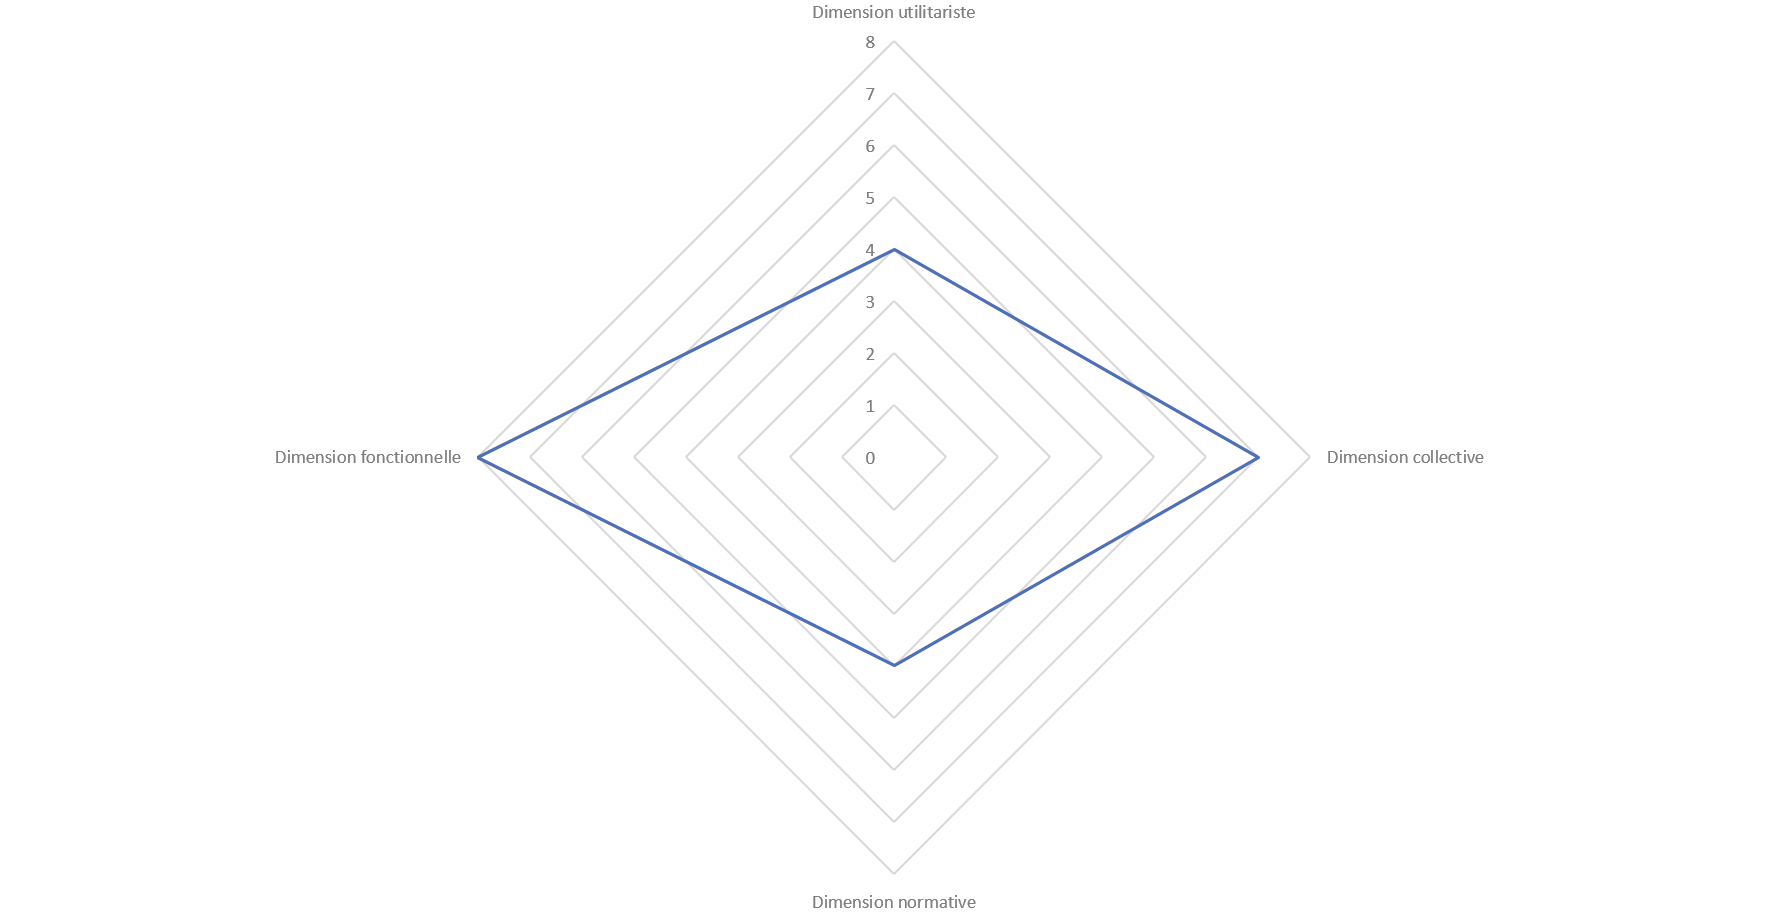
\includegraphics[width=\linewidth]{fig/radars/Air_PACA.png}
        \end{figure}

        L’association appréhende la qualité de l’air comme un enjeu à la fois de santé publique et de préservation de l’environnement. Le cœur de son activité est donc la réduction de la pollution de l’air. Dans ce cadre, l’association se montre très éco-innovante, notamment du point de vue de l’innovation technologique. Air PACA développe des nouveaux médias de communication des données, pour s’approcher d’une information en temps réelle de la qualité de l’air, destinée aussi bien à des particuliers qu’à des organismes privés ou publics. D’autres innovations technologiques portent sur des procédés individuels de mesure de la qualité de l’air, accessibles à tous.
        Ces innovations s’inscrivent pleinement dans une ambition de diffuser le plus largement l’information et de sensibiliser les publics aux enjeux de la qualité de l’air. Pour avoir un impact au niveau de la région, Air PACA porte des éco-innovations institutionnelles en agissant auprès des décideurs en amont des projets d’aménagement du territoire. Au niveau de son fonctionnement, l’association a mis en place l’application de la norme ISO 14001 afin de limiter l’impact de son action (consommation de papier ou d’énergie, gestion des déchets, transports). Ceci prend la forme d’éco-innovations sociales (changements de pratiques des salariés) et organisationnelles (maintien de plusieurs sites pour limiter les déplacements). \\


        La première motivation de l’association dans sa démarche d’éco-innovation est l’amélioration de la qualité de son service. Le secteur de la qualité de l’air connaît un regain d’intérêt mais accuse un retard par rapport à d’autres problématiques comme la question de l’eau. Par conséquent, il est indispensable de suivre les évolutions d’un secteur où beaucoup reste à faire.
        L’évolution des technologies, en particulier dans le champ de la communication, va dans le sens de la volonté de partager et diffuser l’information.
        L’association fait aussi face à une demande croissante des attentes sociétales. Cet intérêt en augmentation se traduit par une hausse importante des demandes d’intervention d’Air PACA, par exemple dans les écoles.
        L’éco-innovation s’inscrit également dans une logique de cohérence entre la mission et les pratiques : l’adoption de la norme ISO 14001 permet à l’association de montrer qu’elle s’applique à elle-même des pratiques responsables avant de les promouvoir aux autres.
        Enfin, le statut associatif pousse Air PACA à démontrer l’efficacité de son action pour maintenir sa légitimité. \\

        Si l’éco-innovation apparaît indispensable pour Air PACA, elle n’est, paradoxalement, pas au cœur de ses missions et donc pas dans son ADN. L’innovation fait donc face à des résistances au niveau de la gouvernance : certaines parties prenantes souhaitent recentrer l’activité sur la mission d’origine, quand d’autres reconnaissent l’intérêt d’éco-innover. Ceci est renforcé par la structure de la gouvernance, au sein de laquelle cohabitent des parties prenantes qui peuvent avoir des agendas très éloignés (un industriel du transport et une association de protection de l’environnement par exemple).
        Au niveau des changements internes, comme la réduction des consommations ou le tri, l’association fait face à des résistances humaines, certains salariés n’étant pas sensibilisés à ces questions et peu enclins à appliquer ces nouvelles pratiques. Des actions de sensibilisation sont donc nécessaires.
        Une barrière conséquente est la dépendance à des financements publics. Alors que la demande augmente, les moyens restent constants et conditionnés à des demandes régulières et chronophages. Le statut d’association est une limite à ces démarches, car il masque la spécificité d’Air PACA et sa mission d’intérêt général.
        Enfin, la dépendance à des partenaires peut également créer des blocages : la collecte des déchets est par exemple rendue difficile par le manque d’engagement de la ville en la matière. De manière plus importante, l’activité est encadrée par un agrément dont les termes peuvent changer rapidement et remettre en question toute l’action innovante de l’association.

    \subsection{AMS Environnement}

        \begin{figure}[h]
            \caption{Identités organisationnelles chez AMS Environnement}
            \label{figure:dimAMSenvir}
            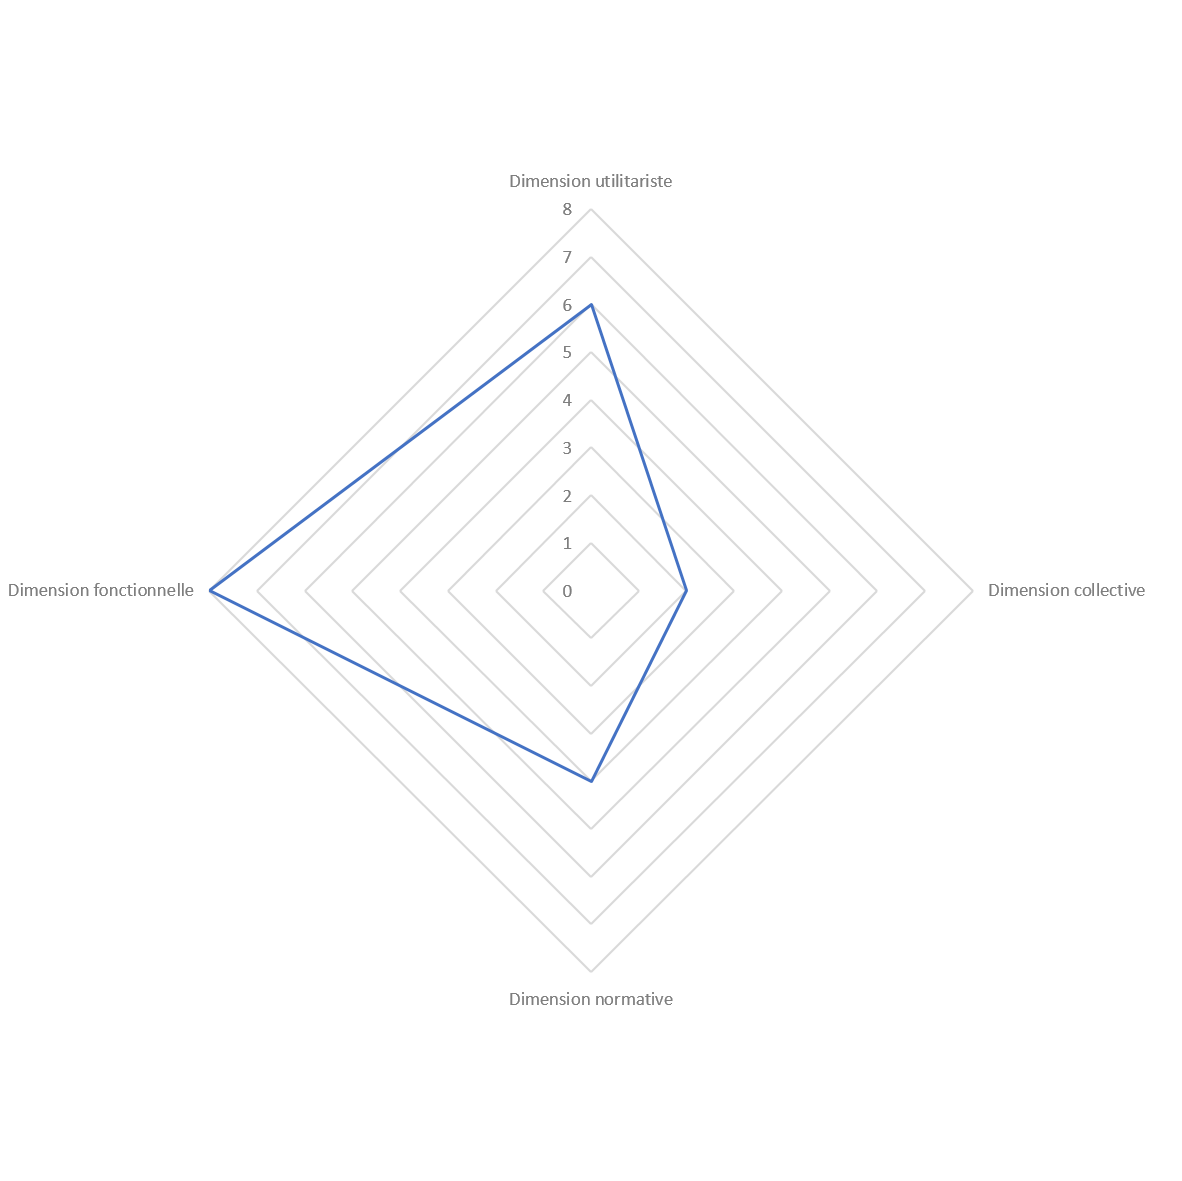
\includegraphics[width=\linewidth]{fig/radars/AMS.png}
        \end{figure}

        AMS Environnement est un chantier d’insertion sous format associatif basé à Aix-en-Provence. Sa mission est de salarier des personnes éloignées du travail pour les ramener vers le monde de l’entreprise. Le support de cette réinsertion est une activité d’entretien et de valorisation des espaces paysagers à destination des collectivités.

        Les différentes caractéristiques de l’ESS sont représentées de manière équilibrée. \textbf{L'identité normative} est marquée par un caractère militant, défendant une vision de l’insertion très centrée sur l’humain. L’association est portée par une volonté d’être acteur du développement durable. Sur \textbf{le plan utilitariste}, AMS revêt un caractère hybride. Le chantier d’insertion adopte un fonctionnement entrepreneurial mettant en avant sa dimension très professionnelle. Ceci est d’autant plus important que sa mission sociale est précisément de professionnaliser ses salariés en insertion. En revanche, 70 \% de ses financements proviennent de subventions. Les difficultés sociales de ses bénéficiaires, leur statut particulier ainsi que la \cit{plus-value humaine} éloignent également l’association d’une logique purement utilitariste. C'est donc avant tout l'\textbf{identité fonctionnelle}, c'est-à-dire la mission d'insertion, qui prime. La \textbf{dimension collective} est principalement marquée par des partenariats avec des acteurs publics lui permettant d’accéder à certains avantages (locaux mis à disposition par la mairie par exemple).  \\


        L’écologie n’est pas au cœur de la démarche de l’association et a été jusqu’ici laissée de côté ou prise en compte de manière marginale. Toutefois, l’organisation s’oriente maintenant vers des activités en lien avec l’écologie, en intégrant notamment les pratiques \cit{zéro-phyto}. En outre, l’association va prochainement acquérir un bâtiment à  basse consommation au Technopole de l’Arbois, justement afin de s’inscrire dans la dynamique environnementale portée à cet endroit.

        L’évolution vers des activités écologiques est principalement stratégique, utilitariste et répond à un enjeu de survie de l’organisation. La conviction de la direction est que leur secteur d’activité va s’orienter vers l’écologie, en particulier s’adressant à des acteurs publics soumis à des normes environnementales importantes dans la gestion de leurs espaces verts. Cette adaptation permet donc de répondre à une demande croissante et de se différencier, d’avoir une originalité par rapport à d’autres entreprises et chantiers d’insertion. La démarche environnementale initiée s’inscrit aussi en lien avec la mission sociale : la dimension écologique est jugée valorisante pour les bénéficiaires, quand l’insertion souffre justement d’une perception négative. L’enjeu des travaux réalisés est toujours expliqué aux employés en insertion afin de valoriser leur action.

        L’orientation écologique ne passe pas par de fortes innovations, mais plutôt par l’adoption de pratiques existantes. L’association ne se positionne pas comme un acteur fortement innovant ; elle fait évoluer son offre dans une direction qui lui semble pertinente stratégiquement. Or, si la demande est croissante, elle n’est pas encore suffisante pour justifier une orientation plus forte en ce sens. En outre, le financement d’activités plus écologiques est jugé encore insuffisant. L’innovation environnementale est également limitée par la grande priorité donnée au projet d’insertion. Le premier défi de l’association est d’avoir une activité réellement \cit{insérante}. C’est sur cet aspect que les efforts ont été principalement concentrés.


    \subsection{Groupe Arborescence}

        Arborescence est un groupe d’économie sociale organisé sous la forme d’une \scic dont sont membres cinq associations et coopératives œuvrant dans des activités autour de l’emploi, de la formation et de l’insertion. La \scic Arborescence assure les fonctions support (direction, administration…) de ces organisations afin de réaliser des économies d’échelle et de bénéficier d’un effet taille.

        \begin{figure}[h]
            \caption{Identités organisationnelles chez Arborescence}
            \label{figure:dimarborescence}
            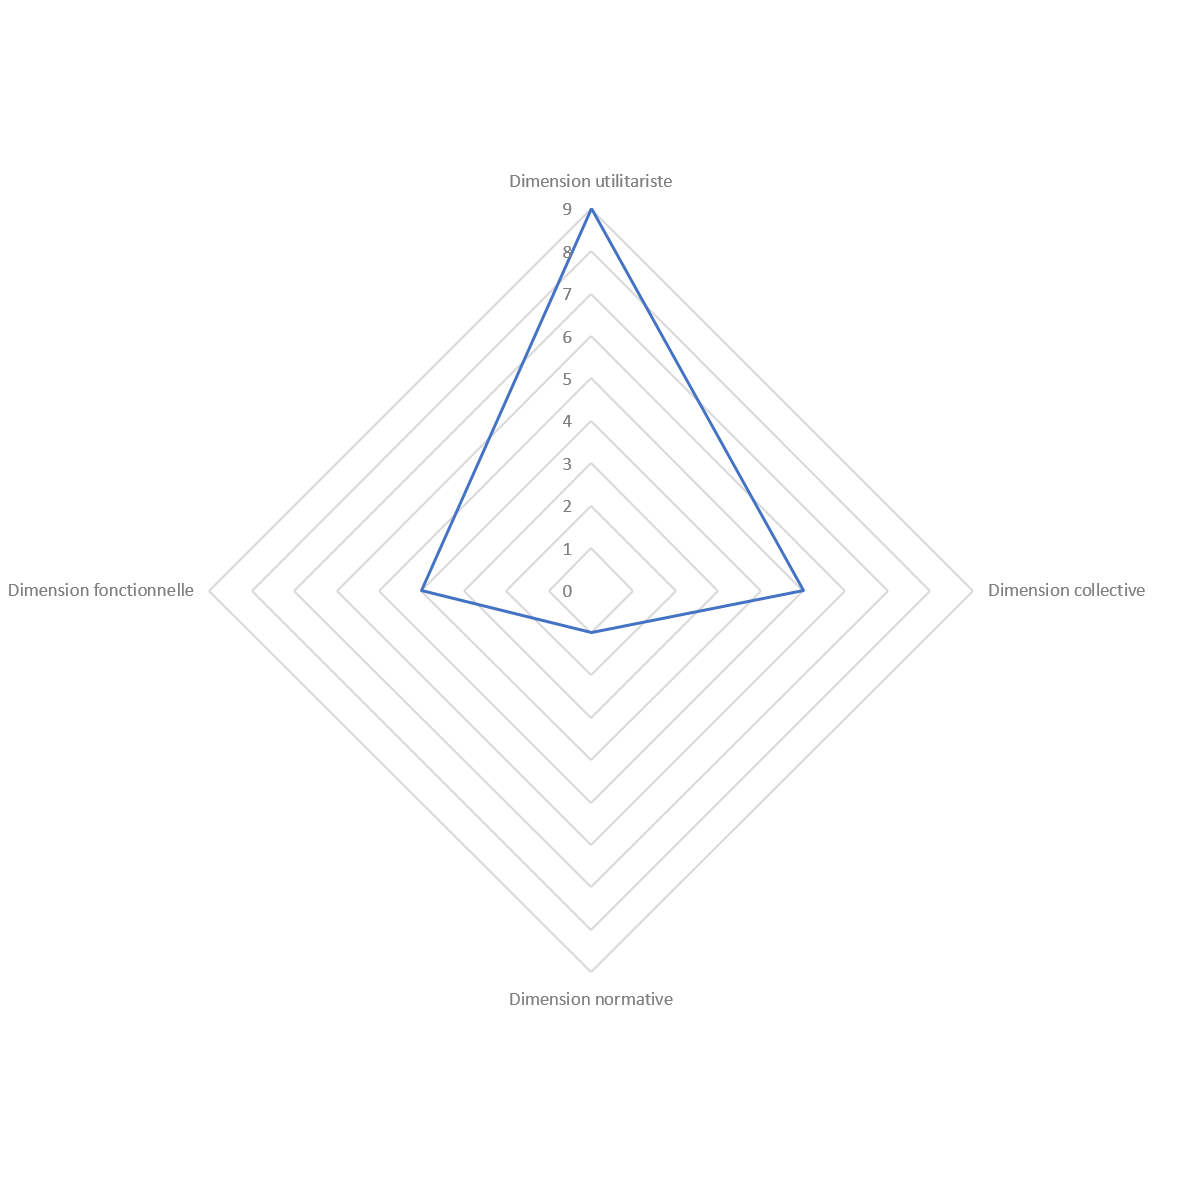
\includegraphics[width=\linewidth]{fig/radars/Arbo.png}
        \end{figure}

        La \scic applique un fonctionnement managérial classique similaire à une entreprise capitaliste (\textbf{identité utilitariste}). La dimension professionnelle est revendiquée et l’organisation formule ses objectifs en termes de résultats et de croissance. La structure coopérative est uniquement adoptée car son métier, l’insertion, est légalement prévu dans le cadre de l’ESS. A ce titre, l’entreprise reçoit des subventions publiques, mais valorise la possibilité d’aller chercher des marchés privés. La \scic se distingue uniquement du secteur classique par un accompagnement renforcé des salariés en insertion et une participation importante des salariés dans la décision. \textbf{L'identité collective} est en effet une caractéristique importante du groupe, la majorité des permanents ayant choisi de souscrire des parts et donc de participer à la gouvernance. \textbf{L'identité normative} est caractérisée par une appartenance historique au mouvement coopératif, sans que cet aspect soit central pour l’organisation et l'\textbf{identité fonctionnelle} repose sur l'activité des chantiers d'insertion. \\

        La stratégie d’Arborescence n’est pas orientée vers les questions environnementales, qui ne sont pas évoquées dans les organes de gouvernance. L’éco-innovation est guidée par les opportunités commerciales et de développement. Une entité du groupe intervient ainsi dans le nettoyage automobile avec des procédés écologiques. Cependant, celle-ci a été intégrée au groupe pour son activité d’insertion et non en raison de sa dimension écologique. Le secteur de l’insertion par les activités environnementales est perçu comme une niche, déjà très occupée par de nombreux acteurs en PACA, et offrant donc peu d’opportunités de développement. Il n’y a donc pas de volonté interne à se montrer éco-innovant.


    \subsection{Enfants et Loisirs}

        Enfants et Loisirs est une association loi 1901 qui détient une crèche et une micro-crèche à Saint-Cannat (13). La mission de l’association est la garde d’enfants la journée, associée à une mission éducative.

        \textbf{L'identité collective} est très importante dans l’association. Les membres sont les parents des enfants bénéficiaires des services de la crèche. Ils sont représentés par un conseil d’administration élu par l’assemblée générale. Bien que les salariés ne soient pas représentés dans la gouvernance, leur rôle est fortement mis en avant et les projets sont mis en œuvre de manière participative. \textbf{L'identité fonctionnelle}, à savoir l'accueil des enfants, la qualité du soin et de la pédagogie est centrale dans l'association. C'est à cette fin que sont mobilisées des valeurs sociales mais aussi environnementales initialement insufflées par la directrice (\textbf{identité normative}). \cit{L'identité utilitariste} est assez peu mise en avant. Les ressources sont majoritairement des subventions publiques mais une partie du service est payée par les membres (les parents). Soumise à des normes et agréée par le Conseil Départemental, l’association adopte toutefois une organisation professionnelle. \\

        \begin{figure}[h]
            \caption{Identités organisationnelles chez Enfants et Loisirs}
            \label{figure:dimenfantsetloisirs}
            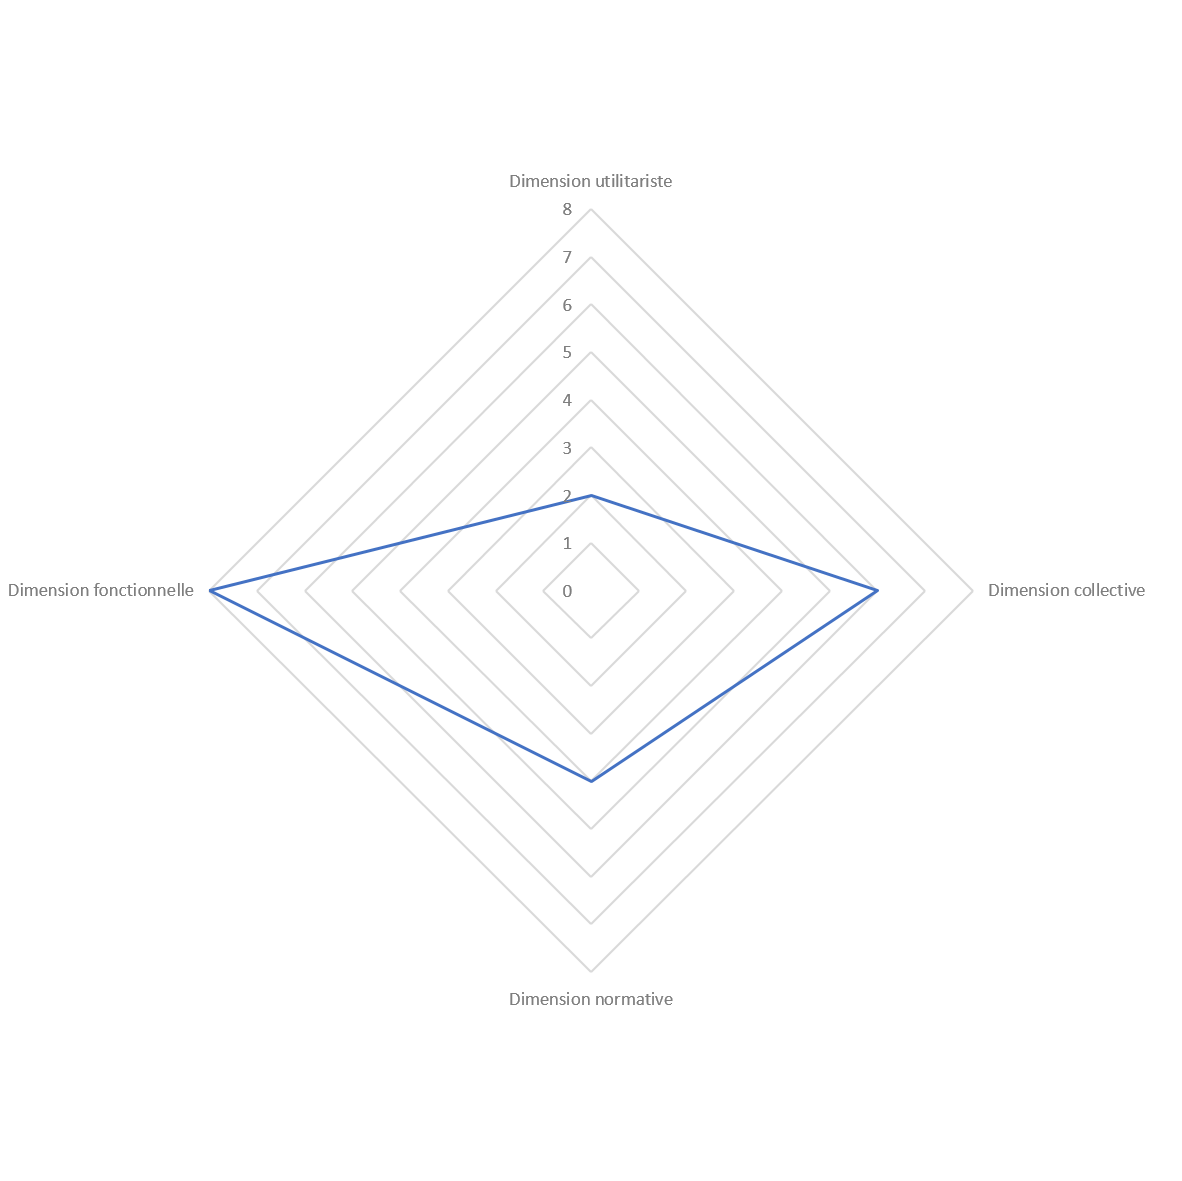
\includegraphics[width=\linewidth]{fig/radars/E&L.png}
        \end{figure}

        Depuis plusieurs années, à l’initiative de l’ancienne directrice de la crèche, l’association s’est engagée dans une démarche écologique valorisée par le label \cit{EcoloCrèche}. Accompagné par l’Atelier Méditerranéen de l’Environnement (AME), l’association a mis en place de nombreux changements dans son organisation et ses pratiques. On peut donner plusieurs exemples d’éco-innovations qui ont été portées. Des innovations technologiques tout d’abord, avec l’investissement dans des appareils de ménage à la vapeur afin de limiter l’utilisation de produits chimiques polluants et l’installation d’un composteur dans la cour. Des innovations organisationnelles également : l’adoption d’une alimentation biologique à la cantine, en s’approvisionnant en partie auprès de petits producteurs locaux ; la fabrication \cit{maison} des produits ménagers ou d’hygiène, mais aussi des peintures, pâtes à modeler, pâtes à sel… ; l’usage de produits de récupération pour fabriquer des jeux ; le recours à des partenaires s’inscrivant dans cette démarche pour proposer des animations aux enfants. De nouvelles activités ont été développées, comme l’organisation d’évènements visant à proposer des produits bio ou écologiques aux habitants du village ; la création d’un potager bio...

        La démarche d’éco-innovation n’a pas été motivée par des considérations marketing ou commerciales, qui ne sont pas un enjeu pour l’association, dans un contexte dépourvu de concurrence. Elle résulte d’une conviction que cette action constitue une responsabilité, voire un \cit{devoir}. L’association est notamment consciente de son rôle éducatif et de l’importance de l’apprentissage dès le plus jeune âge de comportements écologiques. Si l’initiative de cette démarche résultait d’une volonté personnelle, elle a obtenu une adhésion large qui a permis au projet d’aboutir. Cette adhésion s’est retrouvée aussi bien au niveau des membres de l’association (les parents, soucieux du bien être de leurs enfants et de préoccupations environnementales) qu’au niveau des équipes, conscientes de l’importance de la démarche. L’association a également obtenu le soutien de la commune, qui a validé le surcoût budgétaire entrainé par le projet. Le soutien des parties prenantes, mais aussi leur participation active a été un élément clé de la mise en place des éco-innovations.

         Si le projet écolocrèche a été un succès et a permis la mise en place de nombreuses éco-innovations, certains facteurs ont constitué des freins voir des blocages. Tout d’abord, le projet s’est confronté à des résistances humaines : bien que les équipes aient accueilli favorablement le projet, elles ont rapidement redouté une surcharge de travail. En effet, certaines innovations nécessitent un travail important en amont, comme la fabrication de la peinture ou des produits d’entretien. Un travail d’accompagnement et de formation a donc été nécessaire pour faciliter l’acceptation de nouvelles pratiques.  De ces inquiétudes, il a résulté un déséquilibre entre les ambitions de l’AG (les parents) et celles des équipes. Les parents étaient favorables à un projet très ambitieux, allant jusqu’à organiser des actions en dehors de la crèche (actions de sensibilisation auprès des habitants de la commune par exemple). Au contraire, les équipes préféraient un champ d’action plus restreint, centré sur l’enfant et sur les pratiques ayant un impact plus réduit sur la charge de travail. Enfin, la dépendance à certains partenaires réduit aussi les possibilités d’action de l’association, par exemple sur le choix d’une peinture écologique pour des locaux appartenant à la commune.

        Les innovations menées par Enfants et Loisirs vont au-delà de l’activité de la crèche et montrent une volonté de diffuser des pratiques respectueuses de l’environnement. Auprès des membres tout d’abord, c'est-à-dire des parents : des actions ont été menées pour sensibiliser les familles à ces enjeux et les encourager à reproduire des pratiques responsables chez eux. Même au-delà, l’association a souhaité sensibiliser les habitants de la commune, à travers des projets n’ayant pas de lien direct avec l’activité de crèche.

        Le projet Ecolocrèche a entrainé une augmentation de certains coûts (achat d’aliments bio, investissement dans des équipements d’entretien à la vapeur…). Toutefois, ceci ne semble pas avoir constitué un frein. Au contraire, les membres comme les partenaires ont accepté ce surcoût, étant conscients du réel bénéfice pour les enfants. La dimension associative joue ici un rôle essentiel : les décideurs sont motivés par la mission sociale (ici la garde de leurs enfants dans de bonnes conditions) plutôt que par une recherche de gain économique. Cependant, ce projet met en évidence une faiblesse liée à certains types d’éco-innovations, qui est le risque d’un retour en arrière. En effet, certaines innovations, notamment dans les pratiques, ne nécessitent pas seulement un investissement humain pour leur mise en place, mais aussi dans la durée. Par conséquent, le choix a parfois été fait de revenir aux anciennes pratiques. Il est intéressant de noter que les actions qui ont été maintenues sont celles qui touchaient directement à l’enfant, c'est-à-dire qui avaient un lien direct avec la mission sociale de l’association. Les actions plus ambitieuses, comme la sensibilisation au-delà du périmètre de la crèche, ont été abandonnées ou réduites.


    \subsection{Tour du Valat }

        La Tour du Valat est une fondation située au cœur de la Camargue, où elle a vocation à mener des programmes de recherche pour la préservation des zones humides (marais, lagunes, étangs, rizières…). La Tour du Valat est reconnue pour son expertise scientifique. En outre, la fondation dispose d’un domaine important en Camargue, sur lequel elle reproduit les activités traditionnelles camarguaises comme l’élevage, la chasse et la culture, qui sont utilisées comme terrain de recherche et d’innovation.

        La fondation est caractérisée en premier lieu par \textbf{une identité normative et une identité fonctionnelle} étroitement liées. Elles se matérialisent notamment par un fort attachement à des valeurs sociales mais surtout écologiques. L'organisation a été fondée sur la volonté d’un homme d’agir pour préserver la nature. Elle revêt un caractère militant, cherchant à faire évoluer les pratiques en vue de la sauvegarde des zones humides. La fondation a une volonté de réconcilier l’humain et la nature (et non de défendre la nature contre l’humain). \textbf{Le caractère collectif} est un volet essentiel pour la fondation et est en premier lieu matérialisé par des partenariats nombreux. Ceux-ci sont non seulement vecteurs de financements, mais permettent aussi à l’organisation d’exister et de peser institutionnellement. Les projets de la Tour du Valat font fréquemment intervenir des parties prenantes externes (experts, collectivités…) et donnent aussi un rôle important aux salariés. La fondation recherche un équilibre entre l’adoption d’un \textbf{fonctionnement managérial} et la préservation de sa mission environnementale et de ses valeurs. Le financement provient essentiellement des intérêts générés par le capital initial apporté par le fondateur, ainsi que d’une autre fondation qu’il a également créée. Le reste provient de partenariats et d’une activité marchande à la marge. \\


        \begin{figure}[h]
            \caption{Identités organisationnelles chez Tour du Valat}
            \label{figure:dimtourvalat}
            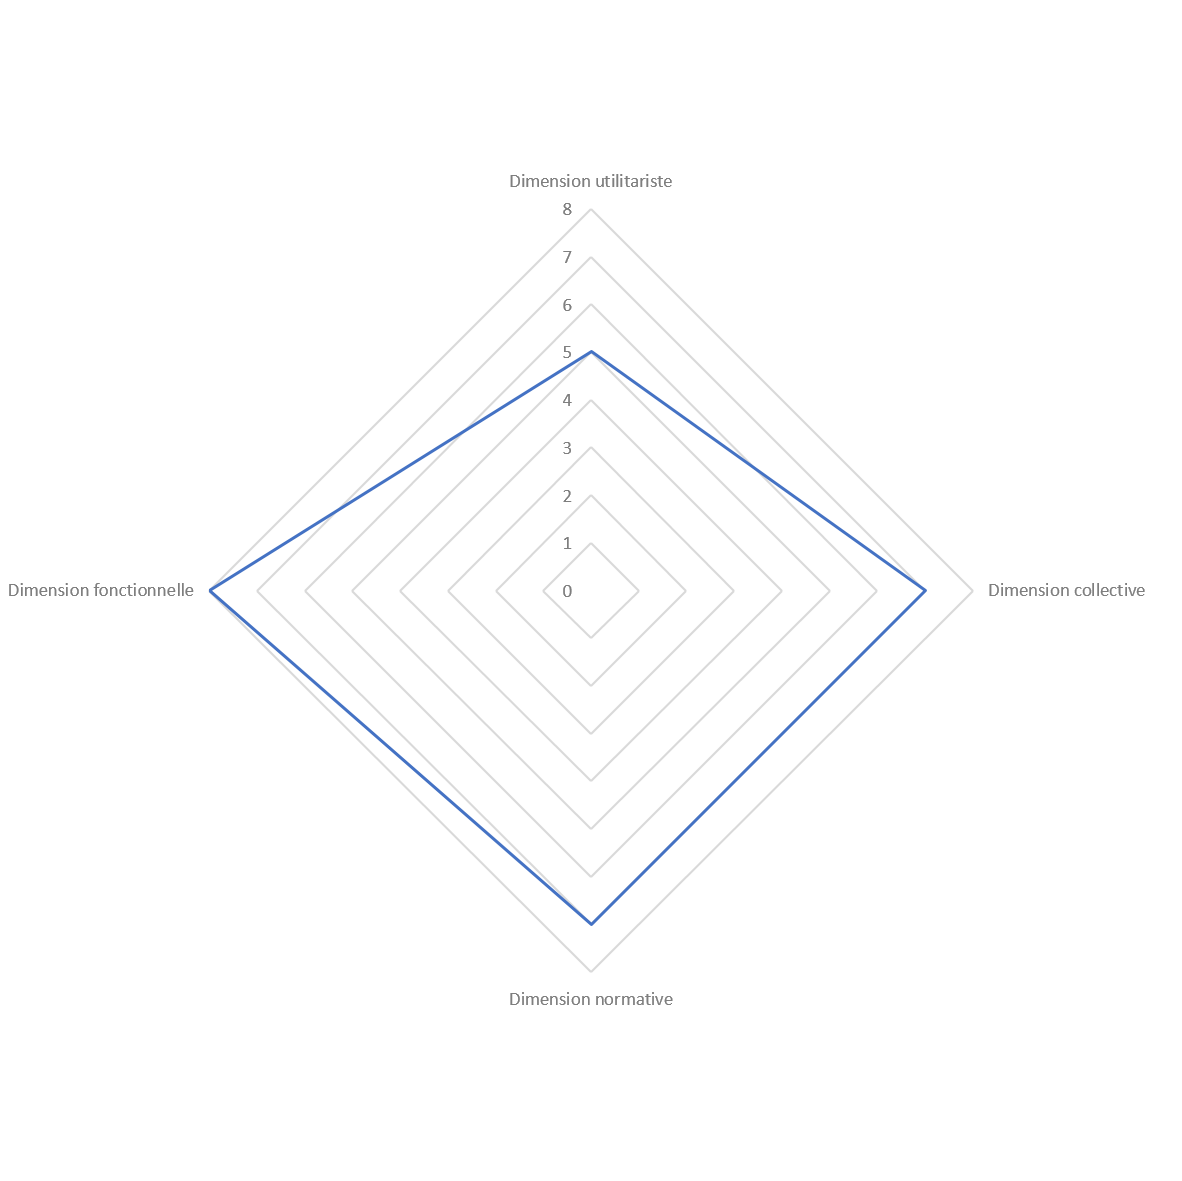
\includegraphics[width=\linewidth]{fig/radars/TdV.png}
        \end{figure}

        La Tour du Valat est par essence engagée dans l’action environnementale. Elle adopte un positionnement très éco-innovant, à différents niveaux. Elle met en place de nombreuses innovations, qu’elles soient technologiques (système de chauffage par chaudière à biomasse, isolation des bâtiments à l’aide de matériaux locaux comme la paille de riz…), sociales (mise en place d’un système de co-voiturage, mise en avant des transports en commun), organisationnelles (valorisation de la visio-conférence pour réduire les déplacements internationaux) ou institutionnelles (le programme de chasse a conduit à faire évoluer la législation en interdisant les balles en plomb pour réduire le saturnisme).

        Ces innovations répondent à plusieurs objectifs. D’une part, elles constituent une mise en cohérence avec les valeurs de l’entreprise et de ses salariés (déterminant interne). D’autre part, il s’agit d’appliquer à soi même ce qu’on préconise pour les autres et donc de légitimer son discours. En outre, ces éco-innovations répondent directement à la mission de l’organisation. Elles lui permettent de se constituer en vitrine, en modèle, pour montrer comment l’activité humaine est réconciliable avec la protection des écosystèmes. Les valeurs partagées au sein de l’organisation ont permis la mobilisation des équipes dans le cadre de ces innovations. Ceci a été un levier important pour la réussite de leur mise en place : certains projets ont ainsi été initiés et menés par les équipes.

        Paradoxalement, les comportements individuels sont aussi un obstacle important à l’éco-innovation, car ils sont parfois en contradiction avec les valeurs prônées. Une autre limite est le financement des éco-innovations, dont certaines ont un coût important. Le manque de moyens a conduit à un projet moins ambitieux et moins innovant pour l’isolation des bâtiments. Enfin, face à des projets très innovants, la fondation a parfois des difficultés à trouver des prestataires ayant l’expertise nécessaire à un coût accessible.

        Une dimension notable est la volonté de diffusion des innovations environnementales, qui résulte de la mission de l’organisation. Son rayonnement porte essentiellement sur le bassin méditerranéen et la fondation encourage l’application de techniques qu’elle a éprouvées dans d’autres écosystèmes comparables.


    \subsection{Provence Forêt}

        Provence Forêt est une coopérative agricole opérant dans la filière du bois et de la forêt. Elle rassemble des propriétaires forestiers dans une perspective de mutualisation des moyens, les parcelles étant généralement trop petites pour être gérées individuellement de façon rentable. Elle assure la valorisation (achat-vente) du bois de ses membres et propose également plusieurs services en lien avec la gestion durable de la forêt. Elle a donc deux catégories de clients : les acheteurs de bois (scieries, papeteries…) et ses membres à qui elle propose des services d’accompagnement.

        \begin{figure}[h]
            \caption{Dimensions de l'ESS chez Provence Forêt}
            \label{figure:dimprovenceforet}
            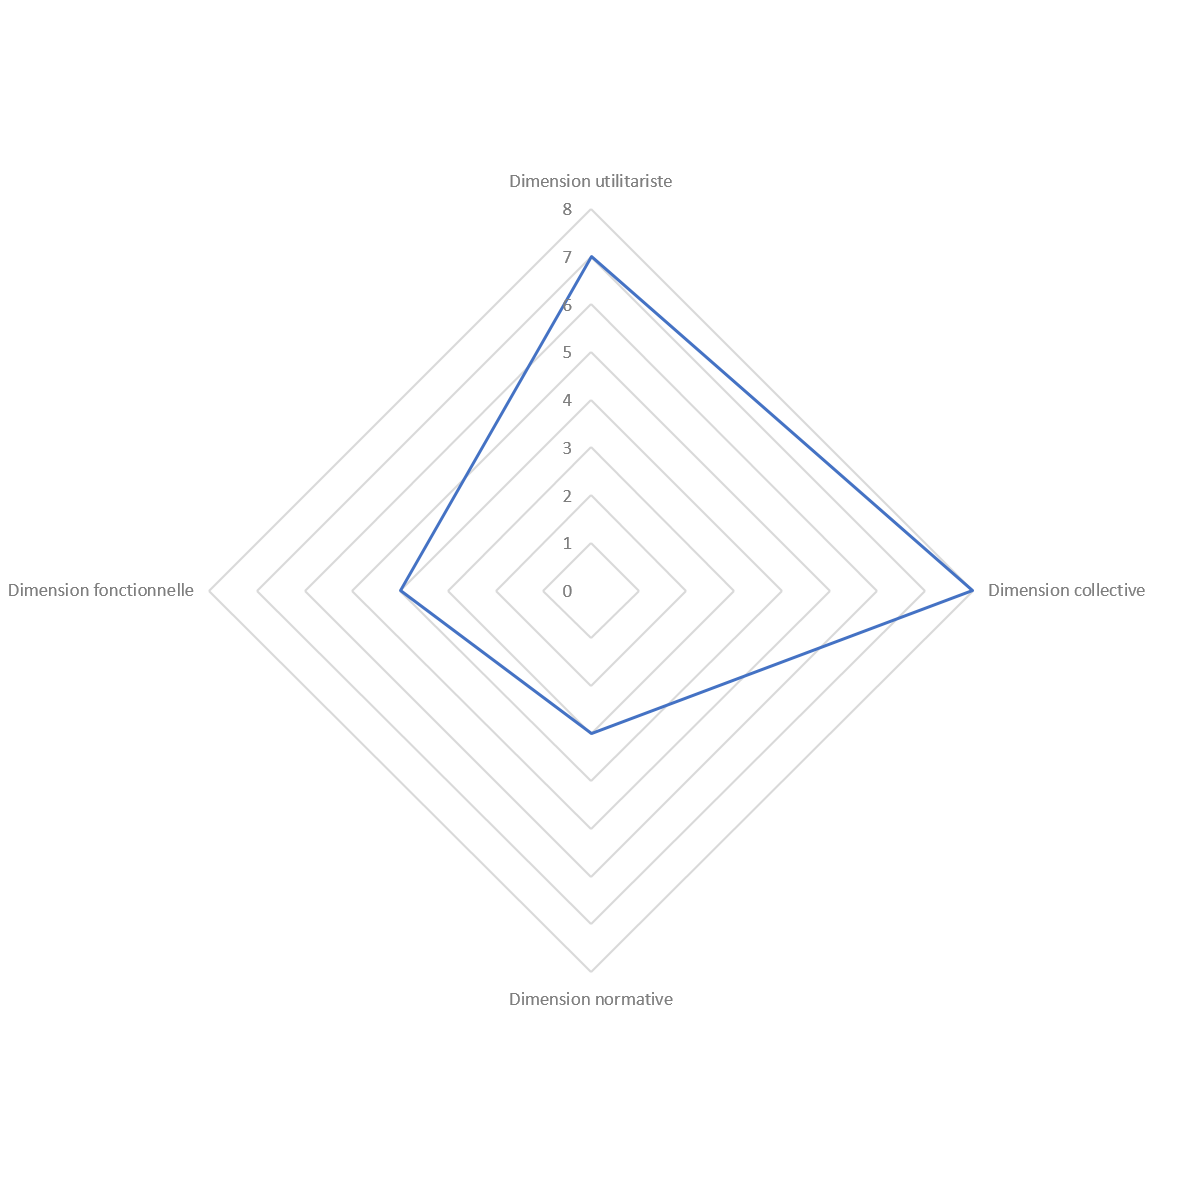
\includegraphics[width=\linewidth]{fig/radars/PF.png}
        \end{figure}
        Assez naturellement pour une coopérative, la dimension la plus marquée est \textbf{l’aspect collectif}. Celui-ci résulte d’abord de la participation des membres, à savoir des propriétaires forestiers, dans la gouvernance. En outre, celle-ci est également ouverte aux salariés (associés non coopérateurs). Mais la coopérative travaille aussi avec de nombreux partenaires. En particulier, l’obtention de plusieurs certifications s’est faite en collaboration avec un groupe de coopératives forestières de différentes régions. L'\textbf{identité utilitariste} est marquée par un fonctionnement entrepreneurial aussi bien dans les ressources financières (seuls 5 \% du chiffre d’affaires provient de subventions) que par un fonctionnement professionnel et très formalisé, organisé selon les normes ISO et PEFC. La structure n'est pas dotée d'une mission sociale ou environnementale, mais plutôt économique (\textbf{identité fonctionnelle}). Le rôle de l'organisation est la fourniture d'un service aux propriétaires forestiers et la valorisation de la filière en région \paca.
        \textbf{L'identité normative} est assez peu représentée, malgré une reconnaissance de la spécificité coopérative et des valeurs sociales et écologiques, existantes mais peu mises en avant. La coopérative insiste toutefois sur son ambition : proposer une gestion durable des forêts. L'appartenance à l'\ess tient surtout dans son format coopératif qui valorise la participation des membres et donne la priorité à la qualité du service et des conditions de travail avant la recherche de croissance du chiffre d'affaires.\\



        La coopérative est confrontée à un contexte environnemental complexe. A la réglementation importante de la filière s’ajoute la superposition des zones environnementales qui sont très nombreuses en \paca et dont il faut tenir compte.  Enfin, les effets du réchauffement climatique, notamment les phénomènes de sécheresse, se ressentent sur les arbres et donc sur l’activité.

        La démarche environnementale de la coopérative se matérialise surtout par l’obtention des certifications ISO14001 et PEFC qui valident une prise en compte de l’environnement et une gestion durable des forêts (éco-innovations de type organisationnel). La plupart des actions menées en faveur de l’environnement s’inscrivent dans le cadre de ces certifications. Celles-ci ont eu principalement des impacts organisationnels, à travers la formalisation de l’activité dans des procédures. Des réorganisations ont été faites pour limiter l’impact sur l’environnement, comme l’optimisation des déplacements en voiture des techniciens pour réduire le kilométrage.

        Les certifications environnementales répondent d’abord à des objectifs financiers et des objectifs d’image. La certification PEFC résulte d’une demande des clients qui ont besoin de se fournir en bois ayant ce label et qu’ils sont prêts à payer plus cher. L’obtention de cette certification en groupe nécessite préalablement une certification ISO. L’ISO 14001 s’est révélée pertinente au vu de l’impact de l’activité sur l’environnement. La démarche répond aussi à un enjeu d’image, la filière bois souffrant d’une mauvaise réputation auprès du grand public. La contestation peut se manifester de manière violente et questionner la légitimité même de la filière, et donc de la coopérative. L’application des normes ISO 14001 et PEFC a aussi été motivée par les bénéfices indirects sur l’activité. Le respect des procédures a conduit à réduire de façon importante le nombre d’accidents, dans un métier réputé dangereux. Les procédures mises en place permettent aussi de garantir le bon respect des réglementations, auxquelles il est facile de déroger involontairement lorsque l’activité n’est pas formalisée. L’obtention des certifications a été considérablement facilitée par la participation au Groupe Coopération Forestière qui avait déjà entamé le processus avant d’être rejoint par Provence Forêt. Les partages d’expériences ont constitué un atout considérable pour faciliter la réorganisation. Enfin, si les motivations sont principalement pragmatiques, l’action environnementale répond aussi à des valeurs environnementales partagée dans la coopérative, notamment au niveau des organes de gouvernance, et la conviction que l’industrie forestière ne doit pas être destructrice de l’environnement.

        La mise en place des certifications a été confrontée initialement à des résistances humaines, venant des salariés inquiets d’une complexification inutile du travail, à travers des procédures et des tâches administratives. D’autres projets d’éco-innovation sont envisagés par Provence Forêt, mais le manque de temps disponible des salariés et de ressources financières ne le permet pas. Ces projets portent notamment sur la recherche de nouvelles façons de planter ou de couper les arbres, ainsi que de nouvelles espèces plus adaptées à l’évolution du climat. Les partenariats viennent parfois compenser ses faiblesses, d’autres coopératives plus anciennes et plus solides financièrement étant fortement engagées dans ces actions de R\&D.

    \subsection{Bzzz}

        Bzzz est une association basée dans le Var, organisée sous la forme d’une AMAP, qui produit du miel et des produits dérivés de l’apiculture. Elle a aussi pour mission d’avoir une action de promotion de \cit{l’apiculture alternative}, de diffusion des connaissances et de militantisme auprès des pouvoirs publics.

        \begin{figure}[h]
            \caption{Identités organisationnelles chez Bzzz}
            \label{figure:dimbzzz}
            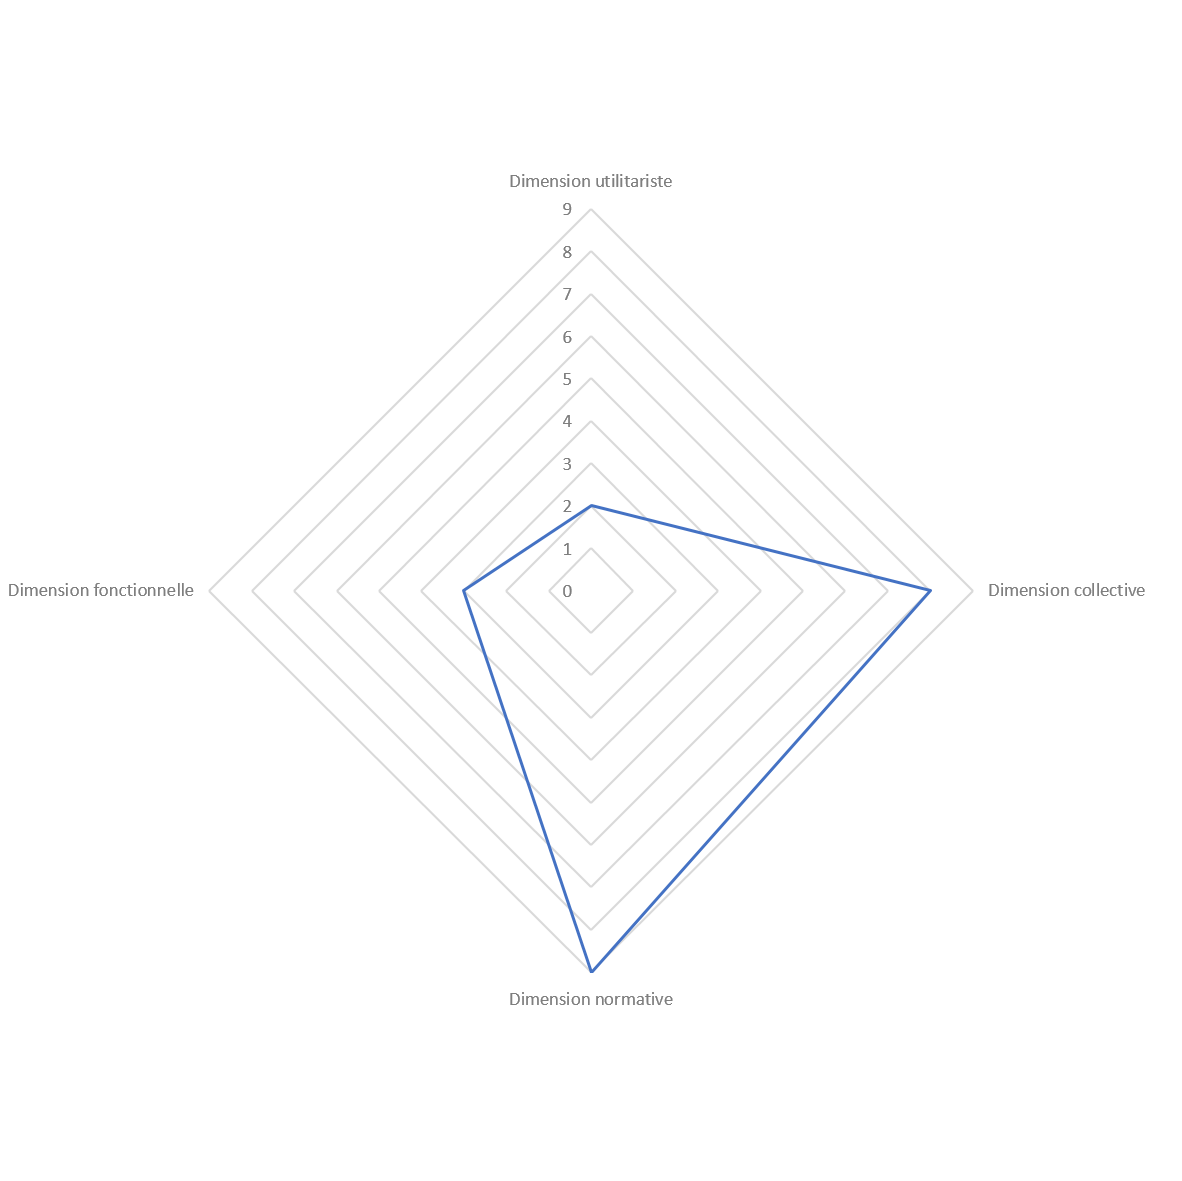
\includegraphics[width=\linewidth]{fig/radars/Bzzz.png}
        \end{figure}

        Bzzz est caractérisée d’abord par une forte \textbf{identité normative et collective}. Sur le plan collectif, l’association attache une importance majeure aux partenariats en particulier dans le milieu associatif, mais aussi auprès des acteurs publics. Ces partenariats permettent d’accéder à des compétences spécifiques, de peser collectivement sur les pouvoirs publics, de diffuser leur modèle et leurs idées ou d’accéder à des financements. L’association s’attache à faire participer à ses actions non seulement les salariés mais aussi des parties prenantes externes. De nombreuses actions sont portées collaborativement avec d’autres organisations. Les partenariats sont également motivés par une vision de l’économie qui ne repose pas sur le principe de concurrence, mais plutôt de collaboration et de co-construction. Ils s’inscrivent donc en lien avec une forte dimension militante de l’association, motivée par des valeurs écologiques et sociales très fortement ancrées. Bzzz porte la vision d’une apiculture alternative, mais aussi d’une autre façon d’envisager l’économie, refusant d’être uniquement guidée par des logiques de performance et de croissance. Ces valeurs sociales, écologistes et collaboratives constituent une finalité pour l'association (\textbf{identité fonctionnelle}), davantage que la production et la vente de miel et produits dérivés. Sur \textbf{le plan utilitariste},  Bzzz cherche un équilibre entre l’intégration de ses valeurs à son mode de fonctionnement et les contraintes économiques auxquelles elle fait face. Ainsi l’association fonctionne avec des salariés, valorise des sources de financement privées et fait preuve de professionnalisme dans la fabrication des produits vendus à ses membres, afin de s’assurer de leur bonne qualité. En revanche, elle revendique un management différent, plus humaniste, et rejette les logiques de performance ou la fixation d’objectifs trop contraignants qui pourraient l’éloigner de sa philosophie. L’association survit en outre grâce à des financements publics, toujours indispensables à ce jour. \\


        L’écologie est au cœur de la mission de l’association et s’inscrit pleinement dans sa démarche militante. Toute son approche de l’apiculture se veut alternative et innovante, et s’inscrit dans l’idée d’un respect de l’humain et de la nature. Par conséquent, de nombreux exemples d’éco-innovations sont observés. La logique de collecte du miel, qui vise à ne pas \cit{voler} aux abeilles ce qui leur appartient, mais à simplement extraire le surplus, se distingue de l’apiculture classique. Bzzz s’appuie sur un cheptel très restreint afin de privilégier la qualité. Des innovations technologiques ont également vu le jour, comme la fabrication d’une miellerie-savonnerie mobile à des fins de production mais aussi à visée pédagogique. Sur le plan institutionnel, l’association a contribué a faire évoluer des réglementations sur l’installation de ruches à Marseille et à réhabiliter une miellerie non utilisée par la ville. Bzzz porte actuellement un projet de création d’une mare et de plantation d’arbres afin de reconstituer un milieu favorisant les pollinisateurs.

        L’éco-innovation est clairement impulsée par l’engagement très fort de l’équipe de Bzzz et par la conviction de la nécessité et de l’urgence d’agir en faveur de l’environnement. Elle est l’essence même de l’association. L’innovation est également indispensable à la survie de l’association qui fait face à un contexte environnemental très difficile. Bien que l’association dispose de peu de ressources financières, des projets parviennent à être portés grâce à des partenariats. La \cit{Bzzz-mobile}, exemple d’éco-innovation technologique, a ainsi été développée à l’aide de plusieurs associations partenaires qui ont apporté les compétences nécessaires ainsi qu’un soutien financier. Les valeurs partagées avec ces partenaires sont un moteur de l’éco-innovation chez Bzzz. Enfin, la spécificité associative de Bzzz lui permet d’accéder à des financements particuliers et d’avoir recours à du crowdfunding en vue de projets donnés. Le projet de rucher actuel s‘inscrit dans le cadre du financement public \cit{Mon Projet Pour la Planète}, qui prend la forme d’une présélection administrative suivie d’un vote citoyen.

        Le modèle de Bzzz est principalement mis en difficulté par un contexte environnemental très difficile qui menace la survie des abeilles. Les sécheresses répétées, l’usage excessif de pesticides dans les exploitations agricoles alentour et la prolifération de prédateurs comme le frelon ont conduit à des récoltes de miel très faibles, voir nulles. L’association est donc confrontée à un enjeu de survie à très court terme et envisage de faire évoluer son modèle. La dimension financière est un enjeu particulièrement important. La difficulté d’obtenir des financements, aussi bien en raison de la charge de travail que des délais d’obtention des fonds, complexifie davantage les choses.

    \transition
    
    Les composants des identités organisationnelles des cas étudiés sont synthétisés dans le tableau \ref{table:synthesedimess}.

    \begin{footnotesize}
     \begin{landscape}
     \begin{longtable}{
         |>{\setlength{\baselineskip}{0.75\baselineskip}}K{0.1\linewidth}
         |>{\setlength{\baselineskip}{0.75\baselineskip}}K{0.2\linewidth}
         |>{\setlength{\baselineskip}{0.75\baselineskip}}K{0.2\linewidth}
         |>{\setlength{\baselineskip}{0.75\baselineskip}}K{0.2\linewidth}
         |>{\setlength{\baselineskip}{0.75\baselineskip}}K{0.2\linewidth}|}

         \caption{Synthèse des cas sous l'angle de l'identité organisationnelle}
         \label{table:synthesedimess} \\ \hline
          \textbf{Source}	& \textbf{Identité utilitariste}	& \textbf{Identité normative}	& \textbf{Identité collective} & \textbf{Identité fonctionnelle}\\ \hline

          \endfirsthead         \hline
          \textbf{Source}	& \textbf{Identité utilitariste}	& \textbf{Identité normative}	& \textbf{Identité collective} & \textbf{Identité fonctionnelle}\\ \hline
          \endhead

        Air PACA
        & Organisation interne classique, formalisation de l'activité à travers des certifications.
        & Mise en avant de l'intérêt général en lien avec l'action environnementale.
        & Gouvernance collégiale (4 collèges : État, collectivités, industriels, associations de protection de l'environnement).
        & Accent mis sur la notion d'intérêt général de la mission de l'association : surveillance et information sur la qualité de l'air.
        \\ \hline

        AMS Environnement
        & Activités menées de façon similaire à une entreprise classique. Recherche de financements de marché.
        & L'humain est mis au centre des missions de l'association, avec une approche personnalisée.
        & La gouvernance intègre des acteurs externes qui apportent des compétences. Cette dimension n'est toutefois pas fortement mise en avant.
        & Les équipes sont prioritairement concentrées sur la mission d'insertion : l'objectif de l'association est d'être \cit{véritablement insérante}.
        \\ \hline

        Groupe Arborescence
        & Fonctionnement similaire  à une entreprise de marché : le statut de coopérative est choisi uniquement pour mener l'activité d'insertion.
        & Le lien avec l'ESS tient dans l'importance donnée au principe de démocratie.
        & Participation de la quasi-totalité des salariés à la gouvernance de l'entreprise. Volonté d'impliquer les équipes dans les décisions.
        & Poursuite d'une mission sociale d'insertion par l'activité économique.
        \\ \hline

        Enfants et Loisirs
        & Organisation professionnelle, soumise à un agrément. Faisant face à peu de compétition, l'association n'est pas dans une démarche productiviste.
        & Les valeurs écologiques sont centrales et matérialisées par le projet "EcoloCrèche".
        & L'association met un accent particulier sur la participation des membres comme des équipes pour mener à bien ses projets.
        & La priorité de l'association est le bien-être et l'éducation des enfants. Cette dimension prime sur les autres aspects.
        \\ \hline

        Tour du Valat
        & Organisation interne classique, recours occasionnel à des financements marchands pour pallier les difficultés de financement de l'organisation.
        & Fondation créée pour défendre des valeurs écologistes et humanistes partagées par les membres de l'organisation. Positionnement parfois militant, volonté de porter un changement sociétal.
        & Gouvernance collégiale faisant intervenir les fondateurs, les pouvoirs publics ainsi que des personnalités scientifiques. Volonté de faire participer les salariés dans les projets de l'entreprise, notamment sur l'éco-innovation.
        & Accent mis sur la production de connaissance scientifique pouvant être diffusées et répliquées dans un but environnemental.
        \\ \hline

        Provence Forêt
        & Revenus essentiellement marchands, formalisation à travers des procédures et des certifications.
        & Valeurs environnementales exprimées en internes.
        & Gouvernance ouverte aux coopérateurs, recours à de nombreux partenariats, en particulier pour l'obtention des certificats à l'aide d'un groupement de coopératives.
        & Activité menée avec la volonté d'avoir une gestion durable des forêts.
        \\ \hline

        Bzzz
        & Dimension utilitariste contestée : volonté de proposer un fonctionnement alternatif, s'éloignant des logiques de compétition.
        & Valeurs sociales et écologiques très fortement exprimées avec au cœur un respect de l'homme et des animaux (les abeilles).
        & Rôle très important des partenariats à des fins d'innovation, de financement mais aussi de diffusion des innovations et de partage des connaissances.
        & Les modalités d'actions (apiculture alternative, management humaniste...) semblent primer sur la mission elle-même (produire du miel et  des produits dérivés).
        \\ \hline

     \end{longtable}
    \end{landscape}
    \end{footnotesize}

    Après cette présentation individuelle de chacun des cas, nous présentons les déterminants de l'action environnementale (section \ref{section:det_act_env}).

                % !TEX root = /Admin/main.tex


\section{Déterminants de l'action environnementale}
\label{section:det_act_env}

Les entretiens réalisés ont permis de mettre en lumière des facteurs qui favorisent l'action environnementale. Il est intéressant de constater que certains de ces atouts peuvent parfois avoir des effets inverses et constituer des barrières à sa mise en oeuvre.

Nous voyons que l'action environnementale répond à des éléments externes, de contexte, à des convictions personnelles des personnes impliquées dans l'organisation, mais aussi dans certains cas à une dimension stratégique et à des aspects économiques. La présence de ces déterminants dans les organisations étudiées est détaillée dans le tableau \ref{table:determinantsEI}.

Dans l'étude de la littérature, nous avons présenté plusieurs typologies de déterminants de l'action environnementale. Cependant, des auteurs \parencite[par exemple][]{dart2010green} suggèrent que d'autres facteurs expliquent l'attitude des \oess  vis-à-vis de l'environnement. Pour cette raison, le codage est réalisé de manière exploratoire, en laissant la place à de nouvelles catégories. Les catégories de déterminants présentées ici ne sont donc pas issues de la littérature, mais bien de l'étude des cas. Nous discutons ensuite de la convergence avec les typologies basées sur le secteur privé lucratif.

\begin{table}[]

    \caption{Synthèse des déterminants de l'\ei dans les 7 organisations étudiées}
    \label{table:determinantsEI}
    \begin{tabularx}{\linewidth}{|L|L|c|c|c|c|c|c|c|}
    \hline
        Catégorie & Sous-catégorie & AP & AMS & GA &  EL & TdV & PF & BZ \\ \hline

        Facteurs externes & Contexte sociétal et technologique &
        + & + & & & & + &
        \\ \hline

        Facteurs externes & Légitimité et statuts de l'ESS &
        +/- &  & & & +/- &  &
        \\ \hline

        Facteurs externes & Contexte législatif &
        - &  & & & &  +  &
        \\ \hline

        Engagement personnel et collectif & Engagement individuel &
        - &  & & +/- & +/- &  +/-  & +
        \\ \hline

        Engagement personnel et collectif & Volonté collective &
        +/- &  &  & +/- & + & + & +
        \\ \hline

        Dimension stratégique & Place stratégique de l'action environnementale &
        + & +/- & +/- & + & + & + & +
        \\ \hline

        Dimension stratégique & Remise en cause des logiques de marché &
        + &  &  & +  & + &  & +
        \\ \hline

        Dimension économique & Financement &
        +/- & - & - &  & - & - & +/-
        \\ \hline

        Dimension économique & Compétitivité &
        & + & - &  &  &  &
        \\ \hline

        \multicolumn{2}{|l|}{Partenariats et collectif} &
        + & + &  & + & + & + & +
        \\ \hline

    \end{tabularx}
    \begin{footnotesize}
         + : effet positif \\
        - : effet négatif \\
        +/- : effet parfois positif, parfois négatif
    \end{footnotesize}

\end{table}

    \subsection{Facteurs externes}
    Nous présentons tout d'abord les facteurs externes qui impactent l'action environnementale dans les \oess.
        \subsubsection{Contexte sociétal et technologique}
        Trois répondants estiment que leur action environnementale s'inscrit dans un contexte sociétal plus général et en lien avec \citit{la montée en puissance de la conscience environnementale des gens} (Responsable Environnement, Coopérative Provence Forêt). Ceci peut se traduire par des demandes explicites ou bien simplement créer un contexte propice à l'action environnementale.  Le directeur d’Air PACA perçoit ainsi \citit{ des attentes aujourd’hui qui sont de plus en plus précises et nombreuses} et qui prennent pour son association la forme de demande d'interventions plus ou moins formelles. Pour l'un des co-président de l'association Bzzz, on est ainsi \citit{en train de surfer sur un moment d’actualité, un moment sociétal plutôt favorable et porteur}.

        Le contexte technologique est également un facteur d'innovation. Le secteur de la qualité de l'air par exemple, sur lequel se positionne Air PACA et qui a été longtemps laissé de côté, fait l'objet d'un intérêt croissant et de nombreuses recherches voient le jour. De nouveaux appareils de mesure se développent et de nouveaux modes d'exploitation des données émergent. L'association se positionne auprès de la communauté scientifique pour suivre ces évolutions.

        \subsubsection{Légitimité et statuts de l'\ess}
        L'appartenance à l'\ess est un facteur ambivalent sur l'action environnementale. Pour certains répondants, elle constitue un atout à travers l'indépendance qu'elle peut offrir. Cependant, cette indépendance connaît des limites et les statuts de l'\ess se heurtent parfois à un manque de reconnaissance et de légitimité.

        Pour le Directeur d'Air PACA, association agréée par l'État et qui remplit une mission de service public, comme pour celui de la fondation Tour du Valat qui intervient fréquemment auprès d'acteurs publics, leurs statuts respectifs assurent une forment d'indépendance et de liberté d'action. Malgré le contrôle exercé sur elle par l'État, Air PACA garde l'initiative des actions qu'elle mène. Cette indépendance s'accompagne également d'une plus grande réactivité, comme le rapporte le Directeur de la Tour du Valat. Une fondation échappe ainsi à la lourdeur administrative d'un organisme public, tout en oeuvrant pour l'intérêt général. Cependant, le constat inverse est fait par la Directrice de l'association Enfants et Loisirs. Certains projets de rénovation utilisant des processus écologiques n'ont pas pu être réalisés, les locaux étant la propriété de la commune. Ce qui est un atout (bénéficier de locaux mis à disposition gratuitement) s'accompagne d'une perte de contrôle qui impacte l'action environnementale. Air PACA s'est heurté à des difficulté similaires lors de la mise en place du processus de gestion des déchets, la Mairie n'offrant pas spontanément la possibilité de collecter le papier à recycler. Enfin la Tour du Valat comme Air PACA mentionnent des difficultés à exister institutionnellement, du fait même de leur statut d'organisme non lucratif. L'agrément public donne à Air PACA une légitimité supplémentaire par rapport à d'autres associations, mais lui donne moins de poids qu'une agence d'État. Elle doit ainsi justifier de son rôle d'intérêt général à échéance régulière pour obtenir les financements dont elle a besoin. Il en va de même pour la Tour du Valat donc l'action n'est pas automatiquement reconnue, malgré la reconnaissance scientifique dont elle bénéficie au niveau international.
        \begin{quotation}
            \citit{Je passe une énergie incroyable à exister institutionnellement, à nouer des relations avec les ministères, avec les institutions régionales, locales etc. sans quoi on n’a pas d’existence par nous-mêmes, on n’a pas d’existence institutionnelle par nous-mêmes, on ne l’a que par les liens qu’on arrive à entretenir} (Directeur, Fondation Tour du Valat)
        \end{quotation}
        Les partenariats noués avec différents organismes sont un moyen de pallier ces difficultés (voir section \ref{av_part}).

        \subsubsection{Contexte législatif}
        L'action environnementale s'inscrit également dans le contexte des lois et réglementations en vigueur. C'est particulièrement le cas pour Provence Forêt qui fait face à un contexte législatif complexe, les zones protégées (de type Natura 2000) étant nombreuses dans la région et pouvant se superposer. Pour la coopérative, la mise en place des procédures en vue de la certification ISO 14001 est un moyen de mieux respecter cette réglementation. Il y a donc une adéquation entre le respect de l'environnement et la prise en compte des contraintes législatives.
        \begin{quotation}
            \citit{On pourrait se dire que c’est simple de suivre la réglementation mais en fait elle est tellement compliquée que grâce à ISO 14001, il y a une procédure qu’on a, ça nous permet de passer tout en revue et de ne pas se tromper} (Responsable Environnement, Provence Forêt).
        \end{quotation}

        La législation, susceptible d'évoluer, peut à l'inverse constituer une contrainte. Air PACA, dont le conseil d'administration donne une place à des représentants de l'État, est dépendante de ces changements, souvent impulsés par l'Union Européenne. Le statut, le financement et la mission même de l'association sont soumis à la législation et l'action environnementale peut être interrompue ou modifiée sur une simple décision de l'État, ce qui fait peser une certaine incertitude sur les projets à moyen et long terme.

    \subsection{L'engagement personnel et collectif}
    Au-delà des facteurs externes, il ressort des entretiens le rôle essentiel de l'engagement des parties prenantes internes à l'organisation, aussi bien au sein de la gouvernance que dans les équipes salariées et bénévoles. La prise en compte de l'environnement est également perçue comme compatible et cohérente avec la mission sociale des organisations de l'\ess.

        \subsubsection{Dimension individuelle}
        Plusieurs répondants ont souligné le rôle de l'engagement personnel de personnes au sein de l'organisation pour impulser des innovations environnementale. Chez Enfants et Loisirs, le projet écolo-crèche qui structure aujourd'hui l'activité a été initialement portée par une directrice sensible à l'écologie. Le \cit{devoir} d'agir pour l'environnement et d'éduquer les enfants à l'écologie est désormais fortement ancré et inscrit dans les documents de l'association. Cette dynamique environnementale est également partagée par les équipes et les parents membres y ont été sensibilisés. Les convictions personnelles des salariés sont également un moteur de l'innovation environnementale à la Tour du Valat. Comme le note le directeur, \citit{les gens qui bossent à la Tour du Valat, la grande majorité ne sont pas là par hasard}, et ainsi sont volontaires pour s'impliquer dans les projets, voire les porter.

        A l'inverse, les comportements humains peuvent également constituer un frein à la mise en oeuvre des éco-innovations. Celles-ci s'accompagnent fréquemment d'une surcharge de travail pour les salariés et exigent une évolution des comportements, parfois mal comprise. Par exemple chez Air PACA, les économies demandées sur les consommations de papier ou la mise en place du recyclage ne correspondent pas toujours aux habitudes individuelles des salariés. Cependant, dans la plupart des cas, ces barrières ont pu être dépassées. L'enjeu est alors le maintien des bonnes pratiques dans le temps, l'engouement et la motivation pouvant s'estomper progressivement.

        \subsubsection{Dimension collective}

        Les valeurs partagées par les membres des organisations peuvent donner forme à une culture commune, favorable à l'action environnementale. Pour plusieurs répondants, cette dynamique entre en résonance avec les principes de l'ESS ou même du développement durable. En effet, certaines organisations parlent plutôt d'un ancrage dans le développement durable (Tour du Valat, AMS Environnement) ou l'économie circulaire (Bzzz) que \cit{d'économie sociale et solidaire}.

        La dimension collective de l'\ess est particulièrement incarnée par l'ouverture des organes de décision à des parties prenantes plus ou moins variées, dans lesquels la voix de chaque personne a le même poids. Le positionnement de ces organes vis-à-vis de l'action environnementale est déterminant. Chez Provence Forêt, la volonté d'adopter un fonctionnement durable et d'adopter des pratiques responsables est fortement portée par le conseil d'administration, c'est pourquoi elle occupe une place centrale dans l'activité. Cependant, l'hétérogénéité des parties prenantes ayant part aux décisions conduit également à des désaccords. Ceci est parfaitement illustré par le fonctionnement d'Air PACA, dont la gouvernance est composée à fois par des industriels, des acteurs publics et des associations de défense de l'environnement. Alors que certains souhaitent valoriser l'innovation autour de la qualité de l'air, d'autres poussent à un retour aux missions d'origine de l'association.

    \subsection{Dimension stratégique}
        \subsubsection{Place stratégique de l'action environnementale}
        Un élément déterminant de l'action environnementale, quasi-tautologique, est la place qu'occupe l'environnement dans la mission de l'organisation. Il va de soi que des organisations comme Air PACA ou la Tour du Valat sont plus sensibles aux enjeux environnementaux, dans la mesure où ceux-ci sont directement liés à leur activité. L'innovation environnementale sert directement l'organisation.
        Cependant, l'action environnementale peut se justifier même lorsque le lien est moins évident. La mission d'une crèche n'a a priori aucun lien avec l'écologie, cependant l'association Enfants et Loisirs y a trouvé une véritable cohérence avec sa mission de soin et de pédagogie. Réduire l'utilisation de produits chimique est bénéfique pour l'environnement, mais aussi pour la santé des enfants. Les activités autour du recyclage ou de la réutilisation peuvent également avoir un véritable intérêt pédagogique. Alors que certaines actions mises en place n'ont pas pu être maintenues dans la durée, celles qui avaient une réelle cohérence avec le coeur de l'activité, c'est-à-dire qui étaient bénéfiques pour les enfants, ont perduré et rencontré une forte adhésion du personnel et des parents. De la même manière, la priorité d'AMS environnement est l'insertion de publics en difficulté. La dimension environnementale présente un intérêt car elle est valorisante, alors qu'un regard négatif est souvent porté sur l'insertion. Elle constitue ainsi un facteur motivant pour les bénéficiaires.

        Néanmoins, l'action environnementale a tendance à être laissée de côté lorsqu'elle ne trouve pas sa place dans l'activité de l'entreprise. Certaines organisations sont tournées en premier lieu vers une mission économique ou sociale. Pour le groupe Arborescence, qui revendique un fonctionnement similaire à celui d'une entreprise classique, l'action environnementale ne peut se justifier que par des opportunités de développement. C'est pourquoi le groupe s'est agrandi d'une société spécialisée dans le lavage écologique d'automobiles. Cependant, la démarche environnementale n'est pas allée plus loin, car les opportunités liées à l'action environnementale sont trop peu nombreuses et constituent une niche déjà très occupée par d'autres acteurs du secteur. Le même constat est partagé par AMS Environnement: si la direction estime que l'écologie pourrait être une direction future pour l'organisation, elle présente encore trop peu d'opportunités économiques :
        \begin{quotation}
            \citit{Le problème c’est qu’aujourd’hui y’a pas suffisamment d’activités où on peut revaloriser nos 30 \% de financements. Il y a peu de besoins écologiques aujourd’hui. Il faut les trouver, il faut les négocier, il faut se battre, il faut être en concurrence avec d’autres structures d’insertion.} (Directeur, Association AMS Environnement).
        \end{quotation}

        \subsubsection{Remise en cause des logiques de marché}
        \label{subsec:contestation_marche}

        Les statuts particuliers de l'\ess permettent aux organisations de se soustraire des logiques purement utilitaristes, voire de remettre en question les schémas de production dominants. Plusieurs des cas illustrent l'effet sur l'action environnementale à des degrés différents. Tout d'abord, les statuts permettent à certaines organisations d'échapper aux mécanismes de concurrence, comme c'est le cas pour Enfants et Loisirs (seule organisation agréée pour l'activité de crèche dans la commune) ou Air PACA (qui bénéficie d'une forme de délégation de service public exclusive). Une forme de concurrence peut apparaître sous des formes plus subtiles, mais de façon moins nettement moins forte que dans le cas des deux structures d'insertion (AMS Environnement et le Groupe Arborescence) ou encore de la coopérative Provence Forêt. Il est donc plus aisé pour les entreprises qui échappent aux pures logiques de compétition de consacrer plus d'efforts à des actions environnementales, y compris lorsque celles-ci ne sont pas rentables ou moins rentables que d'autres investissements. Chez Enfants et Loisir, un certain surcoût a été accepté par les parents et les financeurs publics, comme dans le cas du recours à une alimentation biologique. L'absence de concurrence directe est également bénéfique pour la diffusion des informations relatives à l'action environnementale, comme l'illustre le cas d'Air PACA, qui rend publique et en temps réel une quantité d'information sur la qualité de l'air, utilisable par des acteurs privés à but lucratif. Ce partage d'information, bénéfique pour la société, n'est pas dommageable pour Air PACA puisqu'il s'agit de sa mission même, là où une structure à but lucratif aurait tout intérêt à garder la propriété de ces données.

        Un cas plus marqué de remise en question des logiques concurrentielles est celui de Bzzz. La mission de l'association est justement de proposer un mode de fonctionnement alternatif, faisant passer la dimension écologique et humaine avant la dimension économique. Chez Bzzz, cet aspect est décliné à de multiples niveaux, comme par exemple sur le plan managérial.
        \begin{quotation}
            \citit{On a une forme horizontale avec une logique de collaboration avec notre force de travail qui sont nos salariés. Le conseil collégial est patron de ses salariés et en même temps je pense qu’on est plutôt des patrons… des patrons différents.}  (Co-président, Association Bzzz).
        \end{quotation}
        Cela se manifeste également au niveau des mode de production : dans l'optique de \citit{ne pas stresser les abeilles [...] ne pas traiter avec des produits chimiques, ne pas voler la totalité du miel}, l'association se limite à 50 ruches, quand une exploitation "normale" en compte 200 par ETP.
        Au niveau de la distribution, l'organisation favorise la logique de circuits-courts, limite le recours aux intermédiaires, allant jusqu'à proposer de \citit{sortir du système économique et monétaire} tout en prônant \citit{la bienveillance, la transmission, la communication non-violente, la lenteur} (Site internet).

        L'\ess semble ainsi en mesure de proposer des alternatives au système économique, alternatives qui peuvent s'avérer bénéfiques pour l'environnement. Cette démarche n'est cependant pas systématique. Certaines organisations choisissent au contraire de s'inscrire pleinement dans les schémas économiques classiques, comme c'est le cas pour le Groupe Arborescence. De plus, les contraintes économiques sont omniprésentes et limitent la marge de manoeuvre des \oess.

    \subsection{Dimension économique}
        \subsubsection{Question du financement}
        \label{paragraphe:det_fin}

        L'étude des cas montre que le financement des \oess est une difficulté permanente. Certains dispositifs dédiés à ces structures peuvent néanmoins être mobilisés.

        Six des sept cas étudiés présentent des difficultés à financer leur activité, ce qui conduit à une incertitude sur l'avenir de l'organisation. La question du financement concerne tous les statuts. Pour plusieurs répondants, l'accès aux financements constitue une charge de travail importante et réduit le temps consacré à l'activité, comme l'illustrent les verbatims suivants.

        \begin{quotation}
            \citit{Chacun doit trouver de l’argent dans son domaine, y compris des chercheurs dont le métier n’est pas de chercher l’argent, c’est de chercher, mais néanmoins ici le chercheur il va aussi chercher de  l’argent. Et c’est vrai que trouver 35 \% du budget global c’est une charge, c’est une pression sur les personnes qui est importante } (Directeur, Fondation Tour du Valat). \\
            \citit{Et en fait on se rend compte que c’est toujours impossible, il nous faudra toujours une subvention pour survivre. Et aujourd’hui c’est le gros problème c’est est-ce qu’on va avoir la subvention en 2018 : on ne sait pas ! } (Responsable Environnement, Provence Forêt). \\
            \citit{Ça me dérange un peu, c’est-à-dire que moi j’ai toujours l’impression [...] de passer un temps de rédaction de dossiers, de toujours montrer patte blanche alors qu’on essaye d’être le plus transparent possible. C’est des choses qui prennent énormément de temps, énormément d’énergie.} (Co-président, Association Bzzz). \\
        \end{quotation}

        En outre, l'orientation des organisations vers des problématiques sociales spécifiques impacte négativement la génération de revenus et rend les \oess moins compétitives, comme le remarque le directeur d'AMS Environnement : \citit{du moment vous mettez une plus-value humaine, on ne peut pas être moins chers qu’une autre structure.}

        En revanche, l'économie sociale bénéficie de sources de financements dédiées, souvent orientées vers l'innovation et qui peuvent soutenir l'action environnementale. Les organisations peuvent avoir recours à des dons (Association Bzzz) ou à différents types de subventions ou financements publics (ensemble des organisations du panel). Bzzz recourt également au financement participatif (crowd-funding) pour financer certains projets et répond à des appels à projets consacrés à l'innovation sociale et environnementale. Ces alternatives aux modalités classiques permettent de diversifier les sources de financement, mais demandent aussi un investissement humain important.

        Finalement, la difficulté à financer l'activité conduit les organisations à repenser leurs modèles, parfois au détriment de l'action environnementale :
        \begin{quotation}
            \citit{Régulièrement on fait des arbitrages entre nos ambitions et puis après si on voit qu’on n’a pas les moyens, pas les aides pour nos ambitions, et bien on révise à la baisse nos ambitions tout en essayant d’être cohérents et qu’à terme le retour sur investissement soit pertinent.} (Directeur, Fondation Tour du Valat). \\
            \citit{Nous on a un problème d’argent, on n’a pas assez d’argent pour mettre en place des choses [...]. Nous on a pas mal d’idées mais en fait, très honnêtement, on n’arrive pas à mettre en place.} (Responsable Environnement, Provence Forêt).
        \end{quotation}



        \subsubsection{Recherche de compétitivité}

        La visée sociale plutôt que financière de l'\ess peut constituer un facteur favorisant l'action environnementale, comme indiqué dans la section \ref{subsec:contestation_marche}. Pour autant, certaines organisations s'inscrivent pleinement dans les logiques de l'économie dominante. Le gain de rentabilité potentiel encourage alors l'action environnementale. Les dirigeants constatent que certaines pratiques ont à la fois un coût \citit{environnemental et économique} (Directeur, Association Air PACA). À un niveau plus stratégique, l'écologie ouvre aussi des perspectives de développement et de différenciation par rapport aux concurrents qui intéressent les \oess. Le directeur d'AMS Environnement constate ainsi :
        \begin{quotation}
            \citit{L’écologie c’est une stratégie, oui c’est une stratégie pour durer, parce que je pense que à échéance, on sera obligé d’admettre qu’il va falloir beaucoup de projets écologiques [..]. Notre vision peut être intéressante et stratégiquement on a choisi d’aller au milieu de gens qui réfléchissent sur l’environnement.}
        \end{quotation}

        La limite à l'effet de la recherche de compétitivité sur l'action environnementale se présente dès lors que les dirigeants ne décèlent pas d'opportunités liées à l'écologie. C'est par exemple la raison pour laquelle le groupe Arborescence ne s'oriente pas dans cette direction :
        \begin{quotation}
            \citit{Aujourd’hui, c’est un petit peu les niches, sur les activités de réemploi et tout ça. [...] Il n’y a pas un objectif précis d’aller dans ce domaine d’activité. D’abord, on n’a pas les moyens, et puis il y a quand même pas mal de structures qui y sont déjà aujourd’hui.}
        \end{quotation}

    \subsection{Rôle des partenariats et du collectif}
        \label{av_part}

    La dimension collective des organisations joue un rôle particulier pour l'action environnementale. Elle n'agit pas nécessairement comme un déterminant, ni comme un frein, mais plutôt comme un facilitateur. Plusieurs situations rencontrées par les entreprises de l'échantillon illustrent la contribution d'une approche collective à l'innovation en matière d'environnement.

    Pour certaines organisations, une approche collective est un moyen d'avoir une vision plus large de l'activité environnementale et de lui donner une cohérence générale.
    \begin{quotation}
        \citit{On est dans un métier où les choses vont vite, nous on s’occupe de l’air mais d’autres vont s’occuper de l’eau, des sols, donc on a tout un réseautage qui est nécessaire pour donner une vision d'ensemble de ces questions. } (Directeur, Air Paca).
    \end{quotation}
    De la même façon, s'inscrire dans un cadre collectif permet de mettre en pratique les innovations développées, de faire le lien avec l'action et de diffuser les connaissances. Pour la Tour du Valat par exemple, les partenariats sont indispensables pour insuffler des changements de pratiques à l'échelle internationale. En agissant seule, l'organisation n'a pas la capacité d'être présente sur tous les projets autour des zones humides. Fonctionner en partenariat avec d'autres organisations plutôt que de les voir comme des compétiteurs permet de donner plus de poids aux \eess. C'est en agissant de manière conjointe avec d'autres organisations militantes que Bzzz a pu obtenir des changements de politiques locales en matière d'environnement. \\

    L'action collective facilite également l'accès à des ressources matérielles, humaines ou financières, qui peuvent parfois manquer aux organisations. Des activités de sensibilisation menées par l'association Enfants et Loisirs ont été rendues possible par l'engagement des parents des enfants accueillis par la crèche. L'association Bzzz s'est appuyée sur plusieurs associations partenaires pour achever son projet de miellerie mobile. Ainsi, la Caravanade a fourni des outils et un accompagnement technique.

    Les organisations qui s'inscrivent dans ce type de démarche peuvent aussi bénéficier d'une entraide et d'une mise en commun des connaissances. En passant la certification PEFC dans le cadre d'un groupe de coopératives, Provence Forêt a ainsi profité de l'expérience des autres sociétés engagées dans la démarche. En outre, se sont créées des synergies, chaque coopérative bénéficiant des retours des autres. En outre, alors que Provence Forêt dispose de peu de moyens pour innover, elle peut s'appuyer sur ce qui est fait dans d'autres organisations de ce groupe. \\

    Le collectif se manifeste aussi au niveau de la gouvernance. AMS Environnement souligne ainsi l'intérêt d'avoir des personnes spécialistes des questions environnementales dans son Conseil d'administration, qui peuvent apporter leur expertise et accompagner l'organisation dans une démarche d'innovation. C'est également le cas pour la Tour du Valat qui, en faisant intervenir des élus dans sa gouvernance, se dote d'un soutien institutionnel qui renforce ses possibilités d'agir pour mener à bien sa mission environnementale. \\

    Enfin, pour Provence Forêt, la Tour du Valat ou l'association Bzzz, l'action partenariale constitue aussi une opportunité de réduire les coûts, voire d'obtenir certains financements. La Tour du Valat s'appuie en majorité sur son capital ainsi que sur la participation des autres fondations de son créateur. Toutefois, ces revenus sont insuffisants et la structure doit diversifier les financements. Les conventions de partenariats peuvent apporter une source de revenus complémentaires, tout en permettant la diffusion des actions environnementales de la fondation. Bzzz s'appuie sur la participation du public pour financer certains projets, en recourant à des financements participatifs (crowd-funding). Là encore, l'obtention de revenus permet en même temps de faire connaître l'organisation, ses activités et le modèle alternatif qu'elle propose, tout en permettant aux personnes de s'impliquer dans l'association. De façon plus directe, Bzzz reçoit également des financements de partenaires associatifs. La \cit{Bzzz-mobile} a ainsi été en partie financée par un don des Fonds Epicuriens.

\section{Discussion}
% \reynaud{À mon avis cette partie est un peu plus faible vous auriez dû lire des livres par exemple Mile et Huberman il vous permettrait davantage de justifier votre démarche je pense que la démarche est bonne je la trouve simplement insuffisamment justifiée.

% Pour conclure pourriez-vous dessiner le modèle de Batsal Roth en montrant les spécificités de l' ESS avec un encadré pour la compétitivité un autre pour la responsabilité...}

\label{section:conclu_quali}
    L'étude de cas présentée dans ce chapitre met en lumière la grande diversité des approches de l'action environnementale dans les \oess. Elles réagissent à différents déterminants et adoptent de stratégies environnementales plus ou moins pro-actives. L'étude aboutit à huit propositions, soulignant le lien entre les identités organisationnelles et l'action environnementale. \\

    La section finale de ce chapitre est consacrée à discuter des résultats de l'étude en regard des modèles développés dans la littérature. Nous montrons que les leviers d'action environnementale mobilisés et l'ampleur des efforts fournis s'expliquent par les motivations initiales des entreprises. Nous discutons également d'un élément essentiel pour comprendre l'action environnementale dans les \eess : le positionnement des organisations dans une posture concurrentielle. Alors qu'existe une tendance sociétale forte pour l'\ess à s'inscrire dans le marché et à se montrer compétitive, cette dynamique est plutôt défavorable à une action environnementale forte.


    \subsection{Déterminants et identité organisationnelle}

        Le modèle de \textcite{bansal2000why} offre une grille de lecture intéressante de nos résultats. Les auteurs distinguent trois déterminants de l'action environnementale : la compétitivité, la légitimité et la responsabilité. Le facteur \textbf{compétitivité} désigne la profitabilité attendue de l'action environnementale. les entreprises qui s'inscrivent dans cette démarche cherchent à obtenir des avantages compétitifs, à travers la valeur ajoutée apportée à leurs produits ou à travers de possibles réductions de coûts. Ce facteur ressort dans plusieurs cas étudiés. Il est notamment présent, assez logiquement, dans les organisations ayant une forte identité utilitariste, celles qui se comparent explicitement à des entreprises classiques. Pour celles-ci, la recherche de performance est naturelle, non seulement dans l'action environnementale, mais dans tous les aspects de leur activité. Cependant, la compétitivité environnementale peut aussi être contrainte et répondre aux pressions financières et concurrentielles que rencontrent l'\ess... et qui façonnent aussi l'identité organisationnelle. Les organisations les plus utilitaristes du panel sont aussi celles qui ressentent une concurrence très importante.  En outre, l'effet de ce facteur est limité, conformément à ce que suggèrent \textcite{dart2010green}. Les répondants en recherche de compétitivité identifient peu d'opportunités dans l'action environnementale. Les organisations qui recherchent véritablement un gain de compétitivité en matière d'écologie sont celles qui sont déjà engagées dans l'action environnementale, souvent en lien avec leur coeur de métier.

        \begin{hyp}
        \label{prop:DET1a}
            La recherche de compétitivité est favorable à l'action environnementale dans l'\ess.
        \end{hyp}

        \begin{hyp}
        \label{prop:DET1b}
            La présence d'une identité utilitariste modère positivement l'effet de la recherche de compétitivité sur l'action environnementale.
        \end{hyp}

        \begin{hyp}
        \label{prop:DET1c}
            La difficulté à identifier des opportunités de développement dans l'action environnementale modère négativement l'effet du facteur compétitivité sur l'action environnementale.
        \end{hyp}

        La \textbf{légitimité} est définie par \textcite{suchman1995managing} comme \citit{une perception ou une supposition généralisée que les actions d’une entité sont désirables, convenables ou appropriées au sein d’un système socialement construit de normes, de valeurs, de croyances ou de définitions} (p. 574). Dans l'approche de \textcite{bansal2000why}, le facteur légitimité vise à maintenir la pérennité de l'entreprise en assurant la conformité avec la législation applicable et en maintenant une image en adéquation avec les attentes des parties prenantes concernées. Les résultats vérifient l'effet de la recherche de légitimité sur l'action environnementale dans les \eess. Cette dimension correspond aux facteurs externes identifiés à travers l'étude de cas. Le souci des questions d'image et de perception de l'entreprise par les parties prenantes renvoient à l'identité utilitariste. L'action environnementale vise à pérenniser l'entreprise et à maintenir son activité en répondant aux attentes des clients et des autres parties prenantes. Par ailleurs, plusieurs organisations marquées par une identité fonctionnelle liée à l'environnement soulignent le besoin de cohérence entre leur engagement et leurs actions. En effet, la légitimité d'une organisation à mission environnementale pourrait être contestée si elle même n'adoptait pas des pratiques respectueuses de la nature.

        \begin{hyp}
        \label{prop:DET2a}
            La recherche de légitimité est favorable à l'action environnementale.
        \end{hyp}

        \begin{hyp}
        \label{prop:DET2b}
            L'identité utilitariste modère positivement la relation entre légitimité et action environnementale.
        \end{hyp}

        \begin{hyp}
        \label{prop:DET2c}
            L'identité fonctionnelle modère positivement la relation entre légitimité et action environnementale si la mission est liée à la préservation de l'environnement.
        \end{hyp}

        Enfin, Bansal et Roth identifient une dimension de \textbf{responsabilité} qui désigne une démarche moins pragmatique, mais motivée plutôt par des valeurs et un souci de l'intérêt général. La responsabilité correspond aussi au devoir moral de l'organisation vis-à-vis de la société.
        Ce facteur renvoie directement à la notion d'engagement personnel et collectif mis en évidence par l'étude de cas. Il est à mettre en lien avec l'identité normative des organisations. L'action environnementale des \oess est ici motivée par des convictions portées par des dirigeants ou bien collectivement partagées par l'ensemble des équipes. Le facteur responsabilité a un effet d'autant plus important lorsqu'il est à l'origine même de la création de l'organisation. L'action environnementale n'est alors plus un devoir dont l'accomplissement procure une satisfaction, mais répond à une volonté profonde des personnes. La force de ce déterminant tient dans son caractère incontournable : les organisations centrées sur des valeurs écologiques se montrent très éco-innovantes, y compris lorsqu'elle font face à des barrières importantes. Ceci va dans le sens des résultats de \textcite{marin2015smes}. A partir d'une analyse typologique, les auteurs observent en effet que certaines entreprises (\citit{Revealed barriers cluster}) estiment faire face à des obstacles conséquents à l'éco-innovation, mais s'appuient sur leur expérience pour maintenir des investissements importants. Notre étude montre que l'attachement individuel et collectif à l'environnement est un élément important pour mettre en place des éco-innovations malgré les difficultés rencontrées. L'identité normative est donc un élément favorable à l'action environnementale, à condition que l'écologie soit identifiée parmi les valeurs de l'organisation. \\

        \begin{hyp}
        \label{prop:DET3a}
            L'identité normative est favorable à l'action environnementale si et seulement si l'écologie est identifiée comme une valeur dans l'organisation.
        \end{hyp}

        % \todo[inline]{See recent publications of Bansal}

        Notre étude met également en évidence le rôle de la coopération et du collectif dans l'action environnementale. Peu évoqué dans la littérature sur l'éco-innovation, ce facteur est central dans l'ESS, en particulier, par définition, dans le mouvement coopératif et mutualiste. La gestion démocratique, l'ouverture de la gouvernance à des parties prenantes variées et l'action collective sont des valeurs centrales des \oess. Pour certains auteurs, c'est même la dimension démocratique de l'\ess qui constitue sa réelle spécificité (plutôt que l'aspect non lucratif) \parencite{mccambridge2004underestimating}. Petrella et Richez suggèrent ainsi que le principal enjeu de l'entrepreneuriat social, courant récent de l'ESS, est d'intégrer cette dimension :
        \begin{quotation}
            \citit{ Indeed, if social entrepreneurship is seen as a private innovative solution to new societal challenges unmet by the state nor the market through an original way of combining resources, no alternative model is emerging. But, if social entrepreneurship is led by participative and democratic governance processes that imply a diversity of stakeholders and resources, it can be seen as a building block for an alternative model. } \parencite{petrella2014social}
        \end{quotation}

        La dimension collective est présente dans la plupart des cas étudiés et est fortement valorisée par la majorité des répondants. Elle permet aux organisations d'accéder plus facilement à des financements, à des compétences et à des ressources matérielles et humaines nécessaires à l'action environnementale. Elle joue également un rôle déterminant dans la diffusion de l'innovation environnementale. A travers des partenariats, les organisations obtiennent la légitimité pour promouvoir leurs actions et peuvent accéder à une audience plus importante. L'ESS, historiquement organisée autour d'une approche collective, peut donc jouer un rôle significatif dans la perspective d'un changement d'échelle de l'action environnementale et dans l'optique d'avoir un impact conséquent dans la lutte contre le réchauffement climatique et la préservation de la biodiversité.

         \begin{hyp}
        \label{prop:DET4a}
            L'identité collective est favorable à l'action environnementale si et seulement si les parties prenantes sont sensibles à l'écologie.
        \end{hyp}

\begin{landscape}
    \begin{table}[h]
    \caption{Déterminants de l'action environnementale et identité organisationnelle dans l'\ess}
        \label{table:syntheseDeterminantsIdentite}
        \centering \small
        \begin{tabularx}{\linewidth}{|X|X|X|K{0.5\linewidth}|}
            \hline
             \textbf{Déterminants (modèle de Bansal et Roth)} & \textbf{Facteurs identifiés dans l'étude} & \textbf{Identités associées}  & \textbf{Spécificités de l'\ess}\\ \hline

            Légitimité
            &  Facteurs externes
            & - Utilitariste \newline - fonctionnelle
            & Le facteur légitimité se manifeste par l'attention portée aux parties prenantes. Elle traduit d'une part un souci d'image, d'autre part une volonté d'afficher une cohérence entre l'activité, les valeurs prônées et les actes.
            \\ \hline

            Responsabilité
            & Engagement personnel et collectif
            & - Normative \newline - collective
            & La notion de responsabilité, de rôle éthique à jouer et même de devoir envers l'environnement est présente dans l'ESS. Mais cette dimension doit être complétée par une démarche volontaire, pro-active, répondant à un engagement fort, parfois militant.
            \\ \hline

            Compétitivité
            & Dimension stratégique et dimension économique
            & - Fonctionnelle \newline - utilitariste \newline - normative
            & Le facteur compétitivité dans l'\ess revêt un double aspect. D'un côté, il correspond à l'approche concurrentielle classique, la volonté de croissance et de développement ou simplement de pérennité économique. De l'autre, il répond à une contrainte, face à des difficultés financières. Confrontés à une réduction de leurs financements habituels, les organisations n'ont d'autres choix que de jouer le jeu de la concurrence, au sein de l'\ess mais aussi face au secteur marchand.
            \\ \hline

            & Dimension collective
            & - Collective
            & Ce facteur est nouveau par rapport au modèle. Les cas mettent en évidence l'importance de la coopération pour l'action environnementale. Elle permet notamment de pallier un manque de ressources humaines ou financières.
            \\ \hline

        \end{tabularx}
    \end{table}
\end{landscape}

    \subsection{Impact sur l'éco-innovation}
        Les différents mécanismes discutés dans la section précédente aboutissent à la réalisation d'innovations environnementales dans les organisations étudiées. Les différents types d'éco-innovations identifiés dans la littérature sont représentés dans les \oess. Les organisations développent ou adoptent de nouvelles technologies ou de nouveau procédés afin de réduire leur impact environnemental. Elles mettent également en oeuvre des changements organisationnels et encouragent aussi des changements de comportements des salariés ou des publics cibles (éco-innovations sociales). Certaines innovations dépassent le cadre de l'organisation et prennent la forme d'éco-innovations institutionnelles \parencite{rennings2000redefining}. Si elles sont plus délicates à identifier, on peut toutefois relever des exemples d'innovations \cit{green system} \parencite{arundel2009measuring} qui reposent sur le développement de systèmes de production alternatifs. L'\ess agit donc sur l'ensemble des volets de l'éco-innovation.\\

        Parmi les nombreux exemples d'innovations observés, certains revêtent une portée apparemment plus significative que d'autres. Il est dès lors pertinent de se demander si l'\ess contribue vraiment à l'\ei en apportant des idées nouvelles, répondant ainsi à l'ambition de mouvement de transformation de la société, ou si elle se contente de suivre un mouvement général. \textcite{johannessen2001innovation}, parlant de l'innovation en général, se demandent ce qui est nouveau, à quel point cela est nouveau, et pour qui cela est nouveau. En effet, les exemples d'innovations radicalement nouvelles sont plus rares que ceux d'évolutions progressives, adaptées de procédés existants. Ce qui constitue un changement profond dans une organisation peut être déjà appliquée depuis longtemps dans d'autres structures. Pour les auteurs, ces trois questions aboutissent en réalité à un construit unidimensionnel, qui porte sur la radicalité de l'innovation. Les \oess étudiées mettant en place les innovations les plus radicales sont celles qui sont animées par un engagement individuel et collectif, et notamment lorsque cet engagement est inscrit dans la mission de l'organisation. Par innovations plus radicales, on entend ici celles qui sont nouvelles non seulement à leur échelle, mais aussi d'un point de vue plus général ou du point de vue d'autres organisations, voire qui aboutissent à une remise en cause du système. A l'inverse, les \eess qui ne sont pas prioritairement animées par la cause environnementale, mais par d'autres enjeux (par exemples sociaux), sont plus susceptibles de se tourner vers des innovations moins radicales. Les expériences menées ailleurs, leur adoption par de nombreuses organisations voire l'existence de services publics (par exemple pour le recyclage) permettent une mise en oeuvre facilitée, nécessitant d'y consacrer moins d'efforts et de ressources. \\

        Finalement, un élément émergent de l'étude de cas est la volonté de sensibilisation aux enjeux environnementaux, du partage des connaissances et de la diffusion de l'éco-innovation. A nouveau, cette démarche de diffusion de l'action environnementale est particulièrement saillante chez les organisations fortement sensibles à l'écologie du point de vue des valeurs. Ce phénomène montre que les organisations ne souhaitent pas seulement limiter leur propre impact sur l'environnement, mais aussi généraliser les bonnes pratiques afin d'obtenir des effets globaux. Ceci prend la forme de sensibilisation du grand public et des acteurs concernés, de partenariats permettant de reproduire des innovations développées localement dans d'autres contextes ou sur d'autres territoires. Les \oess, grâce à leur dimension ouverte, la possibilité de faire coexister des parties prenantes variées, ainsi que leur proximité avec la société civile, ont la capacité de créer des synergies et d'insuffler un mouvement généralisé autour des enjeux écologiques. Cependant, cette vision d'une ESS ancrée dans la société, ou \cit{encastrée} selon l'expression de Polanyi, est menacée par la domination écrasante des logiques capitalistes et concurrentielles.

    \subsection{Impact de la concurrence}

        La place de l'\ess dans l'économie fait l'objet d'un véritable débat dans la sphère académique, mais plus largement dans la sphère économique. Doit-elle s'inscrire dans le cadre de l'économie de marché et en accepter le principe de concurrence, ou bien constituer une alternative au modèle dominant ? Notre étude confronte des approches très différentes, parfois choisies, mais parfois contraintes. Les \eess font face à des situations variées. Certaines sont de fait en concurrence directe avec le secteur privé lucratif et n'ont pas d'autre choix que d'être concurrentielles. Les deux cas d'entreprises du secteur de l'insertion, réputé difficile et concurrentiel, en sont d'excellents exemples. Au contraire, certaines organisations, notamment sous format associatif, échappent à cette concurrence en raison de leur statut, par exemple parce qu'elles bénéficient d'un agrément qui leur confère un certain monopole local. Enfin, des organisations choisissent de s'extraire des logiques de marché, au risque de devoir affronter des difficultés supplémentaires et parfois de limiter leurs ambitions. La tendance générale, relevée par plusieurs auteurs, va dans le sens de l'adoption des logiques de marché dans l'ESS. Or ceci est un sujet d'inquiétude pour les organisations, qui voient dans ce mouvement une remise en question de leur capacité d'action, notamment en matière environnementale. \\

        Il apparaît que les \oess qui s'inscrivent dans des logiques de compétitions sont moins éco-innovantes que celles qui échappent à la concurrence. En effet, confrontées à la pression du marché, les entreprises privilégient les éco-innovations qui contribuent à leur positionnement stratégique, mais  y renoncent dès lors qu'elles ne perçoivent pas d'opportunité de développement. Or, les répondants concernés voient plutôt dans l'écologie une économie de niche ou bien des opportunités futures encore peu accessibles.
        Les résultats sont conformes à ceux obtenus par \textcite{mathieu2015les}. Pour les auteurs, les organisations s'inscrivant dans un référentiel financier adoptent plus souvent des stratégies adaptatives, c'est-à-dire plutôt un positionnement de suiveur, quand les entreprises ayant un référentiel durable s'inscrivent dans une stratégie proactive. L'étude menée dans le présent chapitre aboutit à un constat similaire : les \eess dont l'action est motivée par l'engagement individuel et collectif sont plus éco-innovantes que les organisations motivées par la recherche de compétitivité, et sont plus aptes à surmonter les barrières rencontrées. Ceci amène à s'interroger sur l'orientation générale de l'\ess et son rapprochement avec le système capitaliste. Si cette dynamique est jugée plus efficiente en termes de création de valeur par les tenants du libéralisme économique, peut-on espérer la même efficacité en matière environnementale ? \\


        %==)> ce lien dépasse en réalité les questions de financement !!! Mpeme les orgas en difficultés parviennent à éco-innover si elles échappent à ces logiques. Mais celles qui sont sous cette pression ne peuvent pas.

        % \section*{idées en vrac}



        %     Chang et Chen (2013) identifient un lien entre l’identité organisationnelle environnementale et l’éco-innovation

        %     Chang et Chen (2013) : la performance en termes d’éco-innovation des entreprises ayant une identité organisationnelle environnementale s’explique en partie par le gain de légitimité environnementale qu’elles en retirent.

            \chapter*{Conclusion du chapitre \ref{chapitre:casess}}
                \addstarredchapter{Conclusion du chapitre \ref{chapitre:casess}}
                Dans ce chapitre, nous avons présenté les résultats d'une étude qualitative ayant pour objectif de questionner les motivations à l'action environnementale dans l'ESS. La diversité du secteur ressort pleinement de l'étude, alors même que toutes les formes d'organisations n'y sont pas représentées. Plusieurs conclusions peuvent être tirées. \\

Tout d'abord, nous validons l'usage de quatre identités organisationnelles pour caractériser les \oess. Conformément à nos attentes, ces identités peuvent cohabiter, avec généralement une prédominance pour l'une d'elles. Alors que l'\ess est souvent définie par ses valeurs, la dimension normative n'est pas systématiquement au coeur de l'entreprise. Bien entendu, cela ne signifie pas que les \eess en question n'adhèrent pas aux valeurs de l'ESS, mais qu'elles ne se définissent pas et ne s'organisent pas autour de ces valeurs. Leur identité est parfois éloignée des éléments qui sont souvent mis en avant dans la communication promotionnelle de l'ESS. Inversement, la dimension utilitariste occupe dans certaines organisations une place centrale. La performance, la croissance et le management sont des termes parfaitement acceptables et peuvent faire partie intégrante de l'identité des \eess. Cette dimension est parfois volontaire, résultant de conviction que la mission de l'entreprise est mieux servie par une démarche utilitariste, mais aussi parfois subie, en raison de la pression financière qui pèse sur les organisations. En revanche, il est intéressant de noter qu'il existe une dimension \cit{anti-utilitariste}, à savoir des organisations qui rejettent frontalement l'approche capitaliste et managériale de l'entreprise, et adoptent des pratiques à l'opposé de celles du secteur lucratif. Pour certaines organisations, généralement protégées de la concurrence du marché, l'identité fonctionnelle est mise en avant. L'appartenance à l'\ess est statutaire plutôt que revendiquée. L'attention est donnée à la mission d'intérêt général ou collectif plutôt qu'aux modalités de sa mise en oeuvre. Enfin, des organisations affirment leur place dans l'\ess par leur identité collective. Celle-ci se manifeste par l'implication des salariés, voire leur engagement dans les organes de gouvernance, mais aussi par une approche privilégiant les partenariats à la concurrence ou aux rapports clients-fournisseurs classiques. Dans certains cas, l'ouverture se fait à des parties prenantes externes, via les instances de gouvernance ou via l'engagement bénévole ponctuel ou régulier. \\

L'étude valide ensuite la pertinence des modèles d'analyse des déterminants de l'action environnementale existant dans la littérature. L'approche de \textcite{bansal2000why}, qui retient les facteurs de compétitivité, de légitimité et de responsabilité environnementale peut être utilisée. Ce cadre d'analyse nécessite toutefois la prise en compte des spécificités de l'ESS. En particulier, le rôle du collectif, absent des principaux modèles,  est déterminant dans l'action environnementale des \oess. L'adoption d'une démarche collective est bénéfique en termes de ressources et de compétences et permet aux organisations de dépasser les barrières qu'elles rencontrent. De même, l'engagement personnel et collectif, l'adhésion à des valeurs fortes constituent un levier puissant d'action environnementale. Ces facteurs poussent les organisations à rechercher un véritable impact et à mener une action vraiment novatrice, là où les facteurs de compétitivité ou de légitimité sont plutôt vecteurs d'adaptation \textit{a minima}. \\

Enfin, l'action environnementale est rendue difficile par le contexte dans lequel évoluent les organisations. La réduction des financements et les pressions à adopter des \textit{business models} plus rentables sont évoquées par presque tous les répondants. Or les opportunités économiques liées à l'action environnementale ne semblent pas assez incitatives et les efforts nécessaires sont conséquents. Pourtant, les organisations activement engagées dans un processus d'innovation environnementale font état de réels bénéfices. \\


            \chapter{L'action environnementale dans l'ESS : perspectives théoriques et pratiques}
                \label{chapitre:discussion}
                \minitoc \newpage
                % !TEX root = /Admin/main.tex

\section*{Introduction du chapitre}

  Dans les chapitres \ref{chapitre:twitter} et \ref{chapitre:casess}, nous analysons les résultats de deux études et les discutons indépendamment. L'objectif de cette partie est de confronter les conclusions de ces deux études et de présenter une analyse globale de l'ensemble de la thèse. Ce chapitre vise également à prendre du recul sur le travail réalisé et à s'interroger sur ses implications, mais aussi ses limites. \\

  Dans une première section, nous revenons sur les principaux résultats obtenus et en proposons une synthèse. Nous en tirons des implications, non seulement pour les \eess, mais aussi pour la société en général. En effet, nous considérons que la recherche en Sciences de Gestion, en particulier la recherche publique, vise certes à apporter des outils et des connaissances aux entreprises, mais qu'elle est également au service de la société. Il nous semble donc pertinent d'avoir une réflexion sur la façon dont la recherche nous éclaire sur l'organisation de la société et du système économique. \\

  La deuxième section de ce chapitre revient plus en détail sur les aspects académiques de la recherche. Nous nous interrogeons sur la validité interne des études qui sont conduites, et discutons de la pertinence de la généralisation des résultats. Nous nous arrêtons par ailleurs sur les limites de la recherche. Les méthodes utilisés, ainsi que les concepts mobilisés, présentent inévitablement des contraintes qui impliquent une nécessaire prise de précautions dans la lecture des résultats. Nous terminons en ouvrant sur des perspectives d'approfondissement de cette recherche. Nous restons convaincu de l'importance d'étudier l'action environnementale dans l'ESS et encourageons de futures études sur cette thématique encore peu explorée dans notre discipline. Nous détaillons certains éléments de réflexion s'appuyant sur les cadres théoriques de la résistance au changement d'une part, et du business model d'autre part, qui peuvent constituer une base de travail pour de futurs travaux.

\section{Communication et action environnementale dans l'ESS}

  Dans cette première section, nous rappelons les principaux résultats de l'étude et discutons des conséquences qui peuvent en être tirées pour les \oess, mais aussi plus largement pour la société.

    \subsection{Principaux résultats}

        Les deux études qui constituent cette thèse convergent pour montrer que la protection de l'environnement est bien prise en compte dans l'ESS, y compris par des organisations dont ce n'est pas le rôle premier. La majorité des \oess communiquent sur Twitter sur des sujets en lien avec l'environnement et plusieurs cas étudiés font ressortir de réelles préoccupations environnementales. En matière de communication, il semble que les coopératives et les entreprises sociales, qui sont, structurellement, les plus proches de l'économie de marché classique, sont celles qui consacrent la part la plus importante du discours à l'environnement. Cependant, les deux études permettent de constater que leur action environnementale est motivée essentiellement par les opportunités économiques et de développement qu'elle présente ou par le gain de légitimité qu'elle apporte. Elles adoptent alors une stratégie plutôt adaptative (voir tableau \ref{table:strategiesenvir}). Au contraire, les organisations qui se distinguent fortement du secteur lucratif ont un positionnement à la fois plus engagé, prenant part à un débat politique et alertant sur les risques de la non prise en compte de l'environnement. Ces organisations, en particulier celles qui mettent au premier plan leur engagement écologique, vont plus loin dans la démarche et adoptent une stratégie proactive. En outre, malgré les difficultés (notamment économiques) qu'elles rencontrent, elles disposent de nombreuses ressources pour mettre en oeuvre de nouvelles technologies ou de nouvelles pratiques. Les organisations de ce type trouvent un écho important et utilisent des stratégies qui fonctionnent sur les réseaux sociaux. \\
        % \todo[inline]{\textcite{bidet2003insoutenable} ==> isomorphismes, économie plurielle: ESS tiraillée entre isomorphismes et opposition au marché}

        Un autre enseignement de l'étude est celui de l'impact positif de l'identité collective des \oess sur l'action environnementale. Celui-ci ressort en particulier de l'étude de cas : les partenariats ainsi que l'intervention de parties prenantes multiples aux activités et à la gouvernance des organisations renforcent la capacité d'innovation, notamment en matière environnementale. Elle permet de contourner les principales barrières rencontrées par les entreprises dans leur action environnementale. Ce résultat est conforme à ce que trouvent \textcite{mojo2015social} dans le contexte des coopératives. Les auteurs indiquent en effet que l'action collective améliore l'engagement des producteurs dans la protection de la nature. Pour \textcite{musson2018les}, l'effet positif de la dimension collective des coopératives sur l'innovation passe par le renforcement de la confiance. Bien que ce dernier paramètre ne fasse pas partie du cadre de notre étude, il peut effectivement être observé dans plusieurs de cas de l'analyse qualitative. \\


        Cependant, il apparaît que le contexte général dans lequel évoluent les \oess rend difficile l'action environnementale. Elles perçoivent peu d'opportunités de développement en matière d'écologie et souffrent d'un manque important de ressources. Les efforts à mettre en oeuvre pour mener et maintenir une action environnementale efficace sont importants, et nécessitent un engagement humain et financier conséquent. Cependant, celles qui s'y engagent semblent en tirer de réels bénéfices.


        \begin{table}[]
          \centering
          \caption{Stratégies environnementales des organisations de l'\ess}
          \label{table:strategiesenvir}
              \begin{tabularx}{\linewidth}{|K{0.205\linewidth}|X|X|}
                  \hline
                   & \textbf{Attitude opportuniste} & \textbf{Attitude engagée} \\ \hline

                  \textbf{Communication}
                      & Rhétorique positive \newline Discours sur les opportunités, perspectives économiques
                      & Rhétorique négative \newline Discours sur les valeurs et la responsabilité \\ \hline

                  \textbf{Motivations}
                      & Compétitivité, légitimité
                      & Responsabilité (engagement) \\ \hline

                  \textbf{Portée de l'action environnementale }
                      & Niveau organisationnel \newline Adoption d'innovations
                      & Niveau organisationnel et démarche de diffusion \newline Développement d'innovations\\ \hline

              \end{tabularx}
          \end{table}

    \subsection{Implications pour l'\ess et la société}
        \subsubsection{Apports de la pluralité de l'ESS}
        Les différentes approches théoriques de l'\ess révèlent des disparités entre une vision purement sectorielle, la vision d'une économie qui doit s'intégrer au système dominant, ou celle d'une économie alternative. Ces différentes perspectives se retrouvent sur le terrain, et les acteurs de l'\ess perçoivent eux même leur rôle différemment. Les deux études mettent en évidence des organisations qui s'inscrivent dans une perspective économique, pleinement compatible avec le système capitaliste. Elles valorisent une activité économique rentable et un fonctionnement managérial similaire à celui du secteur lucratif. Elles se rattachent à l'\ess par leur mission sociale ou environnementale et par certaines spécificités, par exemple leur caractère coopératif. Inversement, d'autres acteurs se positionnent de manière distincte, voire en opposition, avec le secteur capitaliste. La mission sociale mais aussi les modalités de sa mise en oeuvre sont prioritaires et la dimension économique apparaît comme une contrainte qu'il faut gérer plutôt comme une finalité. \\

        La diversité d'approches dans l'ESS explique en partie les difficultés de visibilité et de légitimation du secteur. Si le positionnement de l'\ess semble manquer de clarté, c'est qu'il doit en réalité composer avec des réalités multiples et parfois contradictoires. Le risque d'une vision unique de l'ESS, institutionnalisée par des lois comme celle de 2014, ou par des rapprochements entre les organismes représentatifs, est d'effacer ou de minimiser certaines approches, certaines façons de voir et de pratiquer l'économie solidaire et sociale. Pourtant, il existe une complémentarité dans ces différentes visions. Un modèle profitable d'entreprises a le potentiel pour redonner du poids à cette économie et pour gagner en efficacité dans le traitement des enjeux sociaux qui manquent encore de réponse. Il contribue aussi à re-légitimer une économie décriée face à une vision largement partagée de l'entreprise, dont le but perçu est avant tout la croissance économique. Mais à l'inverse, il est évident que le système dominant trouve aujourd'hui ses limites, qui se manifestent dans les déséquilibres sociaux et dans la crise environnementale dont les effets se font maintenant ressentir de façon brûlante. Contraindre l'\ess à reproduire les pratiques d'un modèle en crise paraît alors absurde, en particulier quand ses organisations sont capables de produire des alternatives sérieuses et de répondre efficacement à certains enjeux. La recherche va donc dans le sens de Karl Polanyi qui défend une économie plurielle \parencite{laville2003avec}, permettant à plusieurs modèles de s'exprimer et de bénéficier ainsi de leurs avantages. \\

        Au regard de l'action environnementale, la pluralité de l'ESS constitue un véritable atout. Les entreprises sont capables d'appréhender ces enjeux de multiples façons et de mobiliser différents leviers en fonction de leur positionnement. Au niveau de la communication, l'ESS adopte plusieurs approches. Certaines organisations jouent un rôle d'information et sensibilisent le public aux enjeux environnementaux, en lien avec les questions sociales. D'autres, plus engagées, se font le porte-voix d'une partie de la société en alertant sur l'urgence d'agir. Enfin, des entreprises montrent la possibilité d'avancer sur de nouvelles voies de développement, en soulignant que la prise en compte de l'environnement n'est pas opposée au progrès, mais peut être créatrice de valeur. Sur le plan de l'action environnementale, les EESS qui souhaitent s'inscrire dans une démarche écologique bénéficient aussi de leviers intéressants. Les modèles du secteur non lucratif permettent de mener des actions qui ne sont pas justifiées uniquement par les profits : elles peuvent par conséquent mener des projets à caractère environnemental qui ne sont pas particulièrement rentables ou qui n'ont pas d'impact marketing. L'impact environnemental est en lui même une finalité. Pour autant, les OESS ne sont pas aveugles aux opportunités économiques associées à l'action environnementale. Elles présentent en outre des atouts pour capter ces opportunités. \\

        \subsubsection{Soutenir l'action environnementale dans l'ESS}
        Malgré les atouts que présente l'ESS sur le plan de l'écologie, la place des questions environnementales dans l'ESS pose un réel questionnement. En effet, pourquoi l'écologie, qui constitue un enjeu crucial pour l'humanité, n'occupe t-elle pas une place plus centrale dans des organisations qui agissent pour l'intérêt général ? On comprend aisément que certains enjeux sociaux apparaissent plus urgents, plus préoccupants que la protection de l'environnement. Cependant, il existe une forte interdépendance entre les questions sociales et environnementales \parencite[voir par exemple][]{bodin2019improving, reuveny2007climate}. La protection de l'environnement nécessite de repenser l'organisation de la société et les rapports sociaux. C'est donc un enjeu qui concerne l'ensemble de l'ESS, et pas seulement les organisations qui ont une mission environnementale. \\

        Notre recherche apporte certaines indications sur les facteurs qui peuvent soutenir l'action environnementale dans l'ESS. Tout d'abord, l'étude menée sur Twitter met en lumière la place centrale des organismes de représentation, ainsi que celle de certaines grandes organisations, notamment des ONG. Ces acteurs bénéficient donc d'une posture privilégiée et d'une réelle capacité d'influence pour orienter l'ESS vers les questions environnementales. C'est donc en premier lieu à ces organisations de porter un discours écologique. Celui-ci peut viser à éclairer les EESS sur les atouts de l'action environnementale. La recherche de compétitivité est un déterminant de l'action environnementale, mais les organisations peinent à déceler des opportunités. Il est donc possible de jouer sur ce levier en répertoriant les actions environnementales bénéfiques pour les organisations et en leur montrant l'intérêt de porter leur attention sur ces sujets. L'engagement apparaît également comme un puissant levier d'action dans les OESS : les personnes engagées dans l'ESS sont souvent portées par des convictions et s'attachent aux valeurs de l'ESS. Toutefois, l'écologie n'est pas systématiquement identifiée comme un élément central de l'ESS. En cela, les pouvoirs publics ont un rôle à jouer dans la manière dont l'ESS est institutionnalisée. L'article 3 de la loi sur l'ESS prévoit six catégories de \cit{bonnes pratiques} (cf. encadré \ref{encadre:pratiquesess}) dont aucune n'inclut la prise en compte de l'environnement naturel. Cet oubli semble en décalage avec les enjeux actuels et les futures réflexions sur l'ESS pourraient davantage tenir compte des enjeux environnementaux. Enfin, un facteur clé de l'action environnementale est la dimension collective des organisations. Plutôt que d'orienter l'ESS vers des logiques concurrentielles, il convient de valoriser les statuts qui font une place importantes aux parties prenantes. Le modèle des SCIC, dont le nombre augmente rapidement \parencite{observatoire_national_de_leconomie_sociale_et_solidaire_france2017atlas}, pourrait être davantage mis en avant. Il est en effet conçu pour permettre la participation de parties prenantes au sens très large. Les SCIC peuvent également être utilisées pour constituer des groupes d'entreprises (sans liens capitalistiques) ou encore des PTCE (cf. section \ref{ptce}). \\

        \begin{encadre}
        \begin{tcolorbox}
          \caption{Extrait de l'article 3 de la loi de 2014 sur l'ESS}
          \label{encadre:pratiquesess}
          \cit{
            Ces bonnes pratiques concernent notamment : \\
            1 - Les modalités effectives de gouvernance démocratique ;\\
            2 - La concertation dans l'élaboration de la stratégie de l'entreprise ;\\
            3 - La territorialisation de l'activité économique et des emplois ;\\
            4 - La politique salariale et l'exemplarité sociale, la formation professionnelle, les négociations annuelles obligatoires, la santé et la sécurité au travail et la qualité des emplois ;\\
            5 - Le lien avec les usagers et la réponse aux besoins non couverts des populations ;\\
            6 - La situation de l'entreprise en matière de diversité, de lutte contre les discriminations et d'égalité réelle entre les femmes et les hommes, en matière d'égalité professionnelle et de présence dans les instances dirigeantes élues.
          }\\ \parencite{noauthor2014loi} \\
          \end{tcolorbox}
        \end{encadre}

        A un niveau plus micro-économique, la thèse apporte des éléments pour les entreprises de l'ESS qui souhaitent communiquer sur les enjeux écologiques ou mener une action environnementale. Plusieurs stratégies  s'avèrent pertinentes pour communiquer sur les réseaux sociaux, en fonction du positionnement souhaité. Deux approches opposées aboutissent à une bonne performance des tweets. Les organisations peuvent se positionner dans une démarche d'information et de mise en garde sur l'urgence écologique. Dans ce cas, elles adopteront un discours plutôt négatif et n'hésiteront pas à prendre position dans les débats politiques. Inversement, une approche plus économique est possible, valorisant davantage les opportunités de développement. La communication peut souligner la capacité de l'ESS à générer des innovations environnementales et ainsi participer à la création de richesses du pays. Si notre étude s'arrête à étudier la performance des stratégies dans l'absolu, on peut faire l'hypothèse que ces deux positionnements permettent de s'adresser à des publics différents. Un discours négatif, alarmiste et très politique va probablement obtenir l'adhésion de publics militants, déjà sensibilisés et ayant la volonté de s'engager. Inversement, un discours positif, accentuant les alternatives et les voies d'un développement écologique pourra atteindre un public qui s'intéresse aux solutions plutôt qu'à la critique et qui préfère des réponses individuelles aux réponses collectives et politiques. Finalement, du point de vue de l'action environnementale, nous adressons deux recommandations aux entreprises de l'ESS. D'une part, les convictions portées par les membres de l'organisation jouent un rôle important dans l'action environnementale. Leur implication dans les projets d'innovation environnementale est donc à recommander. Non seulement les salariés et les bénévoles peuvent être moteurs dans ces projets, leur participation peut également aider à accepter les changements induits. Dans bien des cas, l'action environnementale est aussi valorisante pour ces personnes. D'autre part, nous suggérons de valoriser l'action collective aussi bien en interne qu'en externe, en multipliant notamment les partenariats. Les échanges entre organisations facilitent l'accès aux ressources nécessaires pour innover et permettent de bénéficier de la complémentarité entre différents types de structures.

        % Pouvoirs publics : https://www.entreprises.gouv.fr/files/files/directions_services/etudes-et-statistiques/prospective/PIPAME-circuits-courts-alimentaires.pdf


\section{Apports, limites et perspectives}

    Dans la section précédente, nous discutons des résultats et des apports de la recherche pour la société. Dans cette section, nous discutons des aspects académiques de la thèse. Nous soulignons ses contributions conceptuelles et méthodologiques, mais aussi les questions de validité, et soulignons les limites inhérentes à la recherche. Nous terminons par la proposition de voies de recherche potentielles.

    \subsection{Principaux apports pour la recherche}

    Sur le plan théorique, cette recherche a permis de tester certains modèles dans le cadre particulier des organisations de l'ESS. En raison de leurs spécificités, notamment le caractère non lucratif de nombreuses organisations, la propriété ou la gestion collective et le recours à des modes de fonctionnement particuliers, on peut s'interroger sur la pertinence de théories et modèles généralement basés sur l'étude d'entreprises classiques. Les chercheurs qui se consacrent à l'entreprise sociale ne s'accordent pas sur la nécessité de développer des théories spécifiques à ce domaine \parencite{valentinov2008economics, dacin2010social, weerawardena2006investigating, santos2012positive}. Ainsi, alors que \textcite{santos2005organizational} proposent un modèle basé sur la création de valeur, ou \textcite{weerawardena2006investigating} un autre reposant sur l'innovation, la proactivité et le management des risques, \textcite{dacin2010social} contestent la nécessité de nouvelles théories. Pour \textcite{yunus2010building-1}, le concept de business model peut être utilisé à condition d'y intégrer une nouvelle composante : le profit social (\citit{social profit equation}). \\

    De la même façon, nous testons un modèle des déterminants de l'éco-innovation et montrons qu'il est adapté pour décrire le comportement des organisations de l'ESS. S'il nécessite quelques reformulations et fait apparaître des éléments spécifiques à l'ESS, le modèle de \textcite{bansal2000why} s'applique bien à ce cadre spécifique. Toutefois, nous le complétons en ajoutant la dimension collective comme déterminant de l'action environnementale dans l'ESS. En effet, l'étude de cas met en évidence un impact fort de la coopération, qu'elle se fasse au niveau de la gouvernance ou à travers des partenariats, voire de l'engagement ponctuel de parties prenantes diverses. Cet élément, central dans l'histoire de l'économie sociale, est essentiel pour acquérir les ressources nécessaires à l'action environnementale. Le volet \cit{responsabilité} du modèle de Bansal et Roth peut également être reformulé. L'action environnementale n'est pas seulement quelque chose que l'on doit faire parce que l'on se sent \cit{responsable} ou parce que cela semble juste. La responsabilité environnementale prend ici la dimension d'un réel engagement, d'une volonté d'agir basée sur des convictions fortes. \\

    Le concept d'identité organisationnelle est déjà mobilisé dans la littérature sur l'ESS, notamment par \textcite{chedotel2012linfluence} ou \textcite{young2000alternative, young2001organizational, young2001organizational-1}. Appliqué à notre recherche, il se révèle efficace pour appréhender l'\ess dans toute sa diversité. Les organisations ayant une forte identité utilitariste sont motivées par des enjeux de compétitivité et se légitiment par leur ressemblance avec le secteur classique. Inversement, celles qui s'appuient sur une identité normative et sont portées par des valeurs peuvent aller plus loin dans l'action environnementale. Pour certaines organisations, la pérennité est presque secondaire, puisqu'une action en contradiction avec les engagements et convictions n'aurait pas de sens. Le recours au concept d'identité permet d'échapper à certaines simplifications, comme l'opposition \cit{marché VS valeurs}. En effet, conformément à \textcite{foreman2002members}, nous observons que les identités cohabitent et que le recours à des pratiques de marché ne s'opposent pas nécessairement à l'engagement. En outre, nous montrons ainsi que l'appartenance à l'\ess a plusieurs formes : elle peut résider dans les valeurs elles-mêmes, mais aussi dans la poursuite d'une mission, indépendamment des modalités d'action, ou dans le caractère collectif de l'activité. Nous complétons donc les approches précédentes en ajoutant l'identité fonctionnelle, déjà identifiée dans nos précédents travaux \parencite{mariaux2018leconomie}, et l'identité collective. Ces deux identités revêtent bien un caractère \citit{central, durable et distinctif} dans l'ESS. La thèse démontre que si certaines organisations valorisent des principes moraux (identité normative) ou plutôt leur rôle économique (identité utilitariste), d'autres se concentrent en premier lieu sur la contribution de leur activité et de leur capacité à trouver des solutions à des problèmes sociaux ou environnementaux (dimension fonctionnelle). Enfin, pour certaines organisations, l'identité collective est incontournable et constitue une caractéristique réellement différenciante de l'ESS. C'est pourquoi elle nous semble incontournable pour rendre compte de ce que représente l'économie sociale.

 \subsection{Validité scientifique de la recherche}

        \subsubsection{Validité interne et externe}

        \textbf{Validité interne} \\
        Nous avons discuté dans le chapitre \ref{chapitre:twitter} des avantages et des inconvénients de la collecte et de l'exploration automatique de texte. Elle permet une bonne reproductibilité de l'étude et limite l'interprétation du chercheur. Le panel d'entreprises est constitué de manière à limiter les biais de sélection : une première sélection est faite à partir de listes institutionnelles d'\eess et d'une recherche par mots clés dans le réseau social lui-même afin de donner un caractère aléatoire. Les analyses visent à réduire l'intervention du chercheur. Cependant, leur caractère quantitatif ne doit pas donner l'illusion d'une parfaite objectivité : l'application des concepts comme les cadres rhétoriques, le pré-codage des données d'entrainement et la détermination du caractère environnemental des tweets impliquent inévitablement des choix et des interprétations. \\

        L'étude qualitative est également conduite de manière rigoureuse afin de permettre des comparaisons pertinentes entre les cas. Tous les entretiens s'appuient sur un même guide et les sujets traités sont donc similaires. Le codage à l'aide de Nvivo permet d'homogénéiser l'analyse des données et d'objectiver dans une certaine mesure l'observation des identités. Nous restons toutefois prudent quant à la quantification des éléments codés qui sont fortement marqués par l'importance donnée à un thème par le répondant et par sa propension à élaborer sur ces sujets. L'apport de l'étude documentaire vient solidifier l'analyse, en apportant des éléments sur l'identité organisationnelle et l'action environnementale qui ne résultent pas de l'interprétation du seul répondant. \\

        \textbf{Validité externe} \\
        Dans quelle mesure les résultats de la thèse peuvent-il être généralisés ? Le premier élément sur lequel on peut s'interroger est celui de la pertinence du contexte français pour étudier l'ESS. Cette économie est historiquement très ancrée dans notre pays. Bien qu'elle soit parfois contestée et, comme nous l'avons vu, poussée à évoluer, elle est omniprésente dans la vie économique et sociale de la France. Nous pouvons donc estimer que la France est un bon terrain d'étude pour s'intéresser à l'ESS. En outre, elle est structurée de manière similaire dans de nombreux pays, en particulier européens, ainsi qu'au Canada. Cependant, l'approche anglo-saxonne est un peu différente, plus centrée sur le secteur non lucratif. Mais de réelles différences peuvent être observés dans \cit{les suds}, selon l'expression de \textcite{laville2016economie}, notamment en Afrique ou en Amérique latine, où l'\ess est prédominée par une économie populaire. Celle-ci s'appuie sur des organisations et des échanges informels, hors de tout cadre institutionnel. Une telle économie existe en France, mais de manière bien moindre, et elle échappe au cadre de notre étude. Par conséquent, on peut s'attendre à des résultats très éloignés en matière d'action environnementale dans de tels contextes. L'économie populaire est souvent une économie de la survie : on peut donc s'attendre à ce que les préoccupations environnementales, plus éloignées du quotidien des individus, soient mises au second plan, voire complètement éludées. \\

        La question se pose également de la généralisation des résultats des études au sein même du contexte de l'\ess dans les pays européens. L'étude du discours sur Twitter est fortement contextualisée. Le réseau social a ses propres codes, ses propres isomorphismes et ses contraintes (notamment en termes de nombre de caractères). L'expression des organisations sur ce réseau est donc simplifiée, synthétisée à travers des messages courts. En outre, la communication sur les réseaux est non vérifiée et non engageante. Il existe cependant un contrôle informel par les utilisateurs eux mêmes : les retours sur Twitter sont immédiats et peu tempérés, ce qui peut inciter les organisations à adopter un discours édulcoré et plus consensuel. Il est donc possible que le discours porté sur Twitter soit différent de celui véhiculé dans d'autres médias et que les résultats en matière de rhétorique environnementale diffèrent. Cependant, la force de l'étude est de s'appuyer sur un échantillon conséquent d'organisations et de porter sur un très grand nombre de messages. Ceci confère aux résultats une validité statistique, confirmée par les indicateurs calculés à chaque étape de l'analyse. \\

        L'étude qualitative, enfin, est la plus difficilement généralisable ; ce n'est d'ailleurs pas sa vocation. Le panel est réduit à sept cas, ce qui ne suffit pas à représenter la diversité de l'ESS, et encore moins à procéder à une généralisation statistique. C'est pourquoi elle aboutit sur la formulation de propositions plutôt que sur des résultats définitifs. Elle a pour objet de révéler des liens entre identité organisationnelle et action environnementale, mais ne permet nullement de les mesurer. Cette étude est donc un appel à davantage de recherches et à l'élaboration d'outils permettant de tester statistiquement la validité des propositions émises.

        \subsubsection{Principales limites}

        Le paragraphe précédent met en exergue certaines limites à notre travail et certaines précautions à adopter pour interpréter nos résultats. La principale limite est la difficulté de la généralisation des résultats liée aux modalités d'étude (une étude menée dans un contexte très spécifique, l'autre portant sur un petit échantillon). D'autres limites doivent être soulignées. \\

        Une d'entre elles porte sur la diversité de l'ESS. Au sein même du secteur associatif, \textcite{valeau2003differentes} souligne les grandes variations qui rendent difficiles les comparaisons. Cette difficulté est d'autant plus forte que nous traitons ici d'un périmètre plus étendu. Le concept d'identité organisationnelle contribue efficacement à rendre compte de cette hétérogénéité. Cependant il se heurte des difficultés d'opérationnalisation, en particulier dans une démarche quantitative. En effet, si nous sommes parvenu à déterminer les identités des \oess à partir des entretiens, l'exercice est moins aisé à mettre en oeuvre à partir d'un questionnaire. A plus forte raison, les données extraites de Twitter, non structurées et non guidées, ne permettent pas d'exploiter réellement ce concept. On est ainsi contraint d'appuyer l'étude sur les statuts organisationnels qui peuvent s'avérer trompeurs et ne reflètent pas effectivement l'identité de l'entreprise. \\

        Une autre limite importante est le recours à des éléments indirects pour évaluer l'action environnementale des organisations. Ceci renvoie à la difficulté de la mesure de l'éco-innovation \parencite{arundel2009measuring, kemp2007final}. En effet, la première étude mesure la prise en compte de l'environnement par le nombre de tweets consacrés à l'environnement. Or, si cela peut rendre compte de l'intérêt de l'association pour les problématiques écologiques, ça n'est pas une mesure de leur engagement concret dans des actions environnementales. Les résultats rendent compte d'une intention davantage que d'une action. En outre, les biais de communication sont importants et l'effet \citit{greenwashing} ne saurait être négligé. Les organisations qui communiquent fortement sur l'environnement sont-elles sensibles à la protection de la nature ou bien... à leur propre image ? La pertinence de l'étude réside donc dans l'interprétation qui est faite de ces résultats : ainsi, on s'attachera moins à la quantité de contenu relatif à l'environnement qu'aux stratégies rhétoriques adoptées. Celles-ci sont plus à même de nous renseigner sur la façon dont l'écologie est perçue par les organisations (risque ou opportunité ?). \\

        Par ailleurs, l'action environnementale doit être distinguée de la performance environnementale. En effet, nous nous basons sur les propos des répondants et sur la documentation pour déterminer ce qui est fait en matière environnementale. Toutefois, nous ne disposons pas d'outils permettant de juger de l'impact réel de ces actions et de juger si elles sont symboliques ou réellement efficaces. Cette limite est d'autant plus importante que la différence entre intention et effet réel est cruciale en matière d'environnement. Les effets cachés sont nombreux et il est peu aisé de choisir le meilleur comportement en matière de protection de la nature. Deux exemples assez courants permettent d'illustrer ce phénomène. Le recours au coton bio pour les vêtements est une pratique d'apparence écologique, mais la production du coton bio est très consommatrice d'eau et a donc un impact sur l'environnement. De même, la voiture électrique permet d'émettre moins de gaz à effet de serre : toutefois sa production nécessite l'extraction de métaux rares et est très coûteuse en énergie. Toute action environnementale nécessite donc une réflexion sur ses effets réels et doit aboutir au meilleur compromis. La thèse s'arrête à l'étape de l'observation des actions menées et ne va pas jusqu'à l'évaluation des effets réels.

    \subsection{Approfondissements et voies de recherche}
        Comme le montre l'analyse de la littérature faite dans les premiers chapitres, la recherche sur la prise en compte de l'environnement dans l'ESS reste à un stade embryonnaire. La thèse apporte de nouveaux éléments, mais soulève également un besoin d'approfondissement. Dans ce paragraphe, nous proposons des pistes de recherche et des théories pouvant porter la lumière sur ces questions.

        \subsubsection{Extension de la thèse}
            Dans la section précédente, nous évoquons les limites de la thèse. Celles-ci soulèvent la nécessité de compléter la connaissance en utilisant d'autres méthodologies. En particulier, il semble indispensable de disposer de données chiffrées plus précises sur l'action environnementale dans l'ESS. Les propositions formulées pourraient notamment être testées de manière statistique. Une telle recherche soulèverait toutefois deux difficultés. D'une part, celle de l'opérationnalisation du concept d'identité, afin d'en permettre la mesure, et celle de l'hétérogénéité du terrain étudié. Nous avons été confronté à ces difficultés dans le cadre d'une étude menée en parallèle de la thèse. Un premier questionnaire, validé par des représentants de fédérations d'\oess, s'est révélé inapproprié pour certaines organisations. A l'inverse, l'usage de questionnaires spécifiques aux différents types d'organisations ne permettrait pas de rendre compte de l'\ess dans son ensemble. \\

            On pourrait par ailleurs s'interroger sur l'effet de l'évolution du contexte général sur les \oess. Au cours des dernières années, on observe une attention grandissante sur le sujet du réchauffement climatique, mais aussi une forte polarisation des opinions sur la question. Peut-on encore ignorer l'écologie lorsque l'on agit au sein de l'\ess ? La pression des parties prenantes sur les questions environnementales est-elle plus forte suite à ces changements et de quelle manière les organisations peuvent-elles y répondre ?  \\

            Le caractère non lucratif (ou à lucrativité limitée) de l'\ess ouvre aussi des voies d'exploration intéressantes quant à son action environnementale. Dans l'économie classique, le rôle de l'entreprise est de gagner de l'argent pour les actionnaires. Dès lors, l'action environnementale est portée par le retour sur investissement espéré (qu'il s'agisse d'un gain financier ou d'un bénéfice en termes d'image et de légitimité). A l'inverse, les \oess peuvent mener des actions sans attendre de retour sur investissement. Là encore, on se demandera quelles sont les attentes des parties prenantes et dans quelle mesure elles peuvent soutenir de telles actions. La théorie des parties prenantes peut également éclairer sur les jeux de pouvoir, l'influence des différents groupes et les effets sur l'action environnementale. \\

            Enfin, en mobilisant la théorie institutionnelle, la recherche pourrait se pencher sur l'impact des isomorphismes sur l'action environnementale. Les modèles de l'\ess sont-ils encore pertinents pour mettre en place une action environnementale innovante ? Ou bien, poussées à ressembler de plus en plus aux organisations du secteur lucratif, les \oess sont-elles vouées à reproduire les mêmes pratiques ? Nos résultats suggèrent que des stratégies proactives sont plutôt menées par des organisations qui, d'une part, s'éloignent d'un pur fonctionnement de marché et, d'autre part, dont les membres sont animés par une forte conscience écologique. \\

            Le cadre théorique du changement organisationnel et celui du \citit{Business Model} peuvent être utilisés pour approfondir ces recherches.

        \subsubsection{Théories mobilisables}
        \textbf{Le changement organisationnel} \\
            L'engagement personnel et collectif constitue un déterminant puissant de l'action environnementale dans les OESS. Cependant, nous voyons qu'il existe aussi des résistances humaines aux changements qu'elle implique. Alors que les organisations doivent s'adapter et se transformer pour répondre aux évolutions du contexte dans lequel elles évoluent, les changements font généralement face à des oppositions de la part des personnes qui subissent le changement \parencite{mariaux2011impact, thomas2011reframing, lines2004influence}.  Si la résistance au changement peut être perçue comme un obstacle à une démarche nécessaire, elle peut aussi être interprétée comme un facteur de succès \parencite{thomas2011reframing}. En effet, pour \textcite{thomas2011managing}, dans un contexte de dialogue, la résistance donne de la matière pour avancer et produire de nouvelles connaissances, et donc finalement faciliter le changement. Plus encore que la communication, la participation active des personnes impactées par un changement dans le processus de mise en oeuvre constitue un facteur de succès des projets organisationnels \parencite{lines2004influence}. \\

            Cette approche soulève une piste d'étude intéressante dans le cadre de l'ESS, où l'implication des salariés, mais plus largement des parties prenantes, tient une position centrale. Or, le changement organisationnel peut être vu comme un ensemble de compromis entre différents acteurs plutôt que comme une stratégie \cit{gagnant-gagnant} \parencite{staw2000what}. Dans cette perspective, le rôle déterminant du collectif dans la mise en oeuvre de projets environnementaux pourrait être expliqué par sa capacité à favoriser le changement. \\

            La réussite des changements organisationnels est également expliquée par un alignement entre les valeurs des membres de l'organisation et l'objectif que l'on cherche à atteindre \parencite{burnes2011success}. Notre étude de cas va dans le même sens et les valeurs partagées au sein de l'organisation jouent un rôle favorable à l'action environnementale. Il serait intéressant d'étudier plus en détail les valeurs individuelles des personnes travaillant dans les \eess et de s'interroger sur l'alignement avec les objectifs environnementaux. Si on peut sans trop de risque parier sur la sensibilité écologique d'une personne engagée dans une ONG de protection de l'environnement, qu'en est-il d'un employé d'une mutuelle, d'une coopérative agricole ou d'une association humanitaire ? \\

        \textbf{Le business model durable} \\
            D'abord exploité sur le terrain, notamment porté par le regain d'intérêt pour l'entrepreneuriat, le concept de Business Model a fait l'objet de nombreuses publications au cours des dernières années. Ayant été mis en pratique avant d’être clairement défini théoriquement, il a souffert d’une certaine confusion sur le plan conceptuel. Il peut être vu comme \citit{des histories qui expliquent comment les entreprises fonctionnent} \parencite{magretta2002why} ou, plus pragmatiquement, comme \citit{les choix qu’une entreprise effectue pour générer des revenus} \parencite{lecocq2006business}. Malgré des divergences sur la définition et les composantes du Business Model, les auteurs s’accordent sur sa finalité : expliquer comment les organisations créent de la valeur et s’en approprient une partie. Si l'on écarte la dimension d'appropriation de la valeur, ce concept est parfaitement applicable à l'ESS, y compris au secteur non lucratif. En outre, les considérations sociales et environnementales s'intègrent parfaitement à ce cadre d'étude \parencite{birkin2009new, bocken2014literature, boons2013business, upward2016ontology}.\\

            L'angle du Business Model présente un vrai potentiel pour comprendre comment les \oess s'adaptent à l'évolution du contexte et répondent aux injonctions à se rapprocher des entreprises capitalistes. Il permet d'avoir une approche globale de l'organisation et de mettre en évidence les schémas par lesquels les organisations peuvent continuer à créer de la valeur sociale et environnementale tout en assurant leur modèle économique. Une telle étude peut aboutir à la constitution d'une typologie d'\oess en fonction du modèle adopté. Il est alors envisageable de questionner la pertinence des différentes catégories au regard des objectifs à atteindre. De manière intuitive, la thèse permet d'identifier plusieurs business models dans l'\ess (cf. tableau \ref{table:bm_ess}). \\


            \begin{table}
              \caption{Une classification des business models de l'\ess}
              \label{table:bm_ess}
              \begin{tabularx}{ \linewidth }{ |K{0.17\textwidth}
                                              |K{0.17\textwidth}
                                              |K{0.17\textwidth}
                                              |K{0.17\textwidth}
                                              |K{0.17\textwidth}
                                              |
                                            }
                \hline

                \multirow{2}{*}{}
                &	\multicolumn{2}{|C|}{\textbf{Modèles basés sur le marché}}
                & \multicolumn{2}{|C|}{\textbf{Modèles non basés sur le marché}}
                \\ \cline{2-5}

                &\textbf{Business Model entrepreneurial}
                & \textbf{Business Model coopératif}
                & \textbf{Business Model militant}
                & \textbf{Business Model associatif} \\ \hline

                \textbf{Finalité} & Economique et sociale & Economique et sociale  & Sociale & Sociale \\ \hline
                \textbf{Initiative} & Individuelle & Collective & Collective & Collective \\ \hline
                \textbf{Prix} & Prix de marché & Prix de marché & Prix non basés sur le marché & Prix non basés sur le marché \\ \hline
                \textbf{Coûts financés par les revenus de l'activité} & Oui & Généralement oui (mais subventions possibles) & Généralement oui (mais subventions possibles)  & Non (financement par des dons, adhésions et subventions)\\ \hline
                \textbf{Capture de la valeur (recherche de profit par les investisseurs)} & Limitée & Limitée & Nulle & Nulle \\ \hline
                \textbf{Ressources humaines} & Salariées & Salariées & Principalement salariées & Salariées et/ou bénévoles \\ \hline

              \end{tabularx}
            \end{table}

          Cette classification embryonnaire ne mobilise pas toutes les composantes du business model, mais celles qui sont le plus souvent utilisées. Le modèle entrepreneurial se développe avec le concept d'entreprise sociale. L'idée est de répondre à un besoin social ou environnemental à travers une activité économique rentable, adoptant les \cit{bonnes pratiques} managériales. Seule la finalité et une moindre recherche de profits différencient ce modèle de l'entrepreneuriat classique. Le modèle coopératif est logiquement celui des coopératives. La finalité économique est bien présente, mais la grande différence avec le précédent est l'entrepreneuriat collectif. Le modèle militant se caractérise également par un entrepreneuriat collectif, mais se distingue par un modèle économique hors-marché. Les organisations peuvent proposer des prix plus élevés - mais considérés comme plus justes - ou au contraire des prix plus faibles pour donner accés à des biens et services à des populations défavorisées. Enfin, le modèle associatif (qui mériterait certainement une sous-catégorisation) se caractérise par la non lucrativité, un modèle économique ne dépendant pas strictement des ressources issues de l'activité et le possible recours au bénévolat. \\

          Alors que les acteurs de l'\ess prétendent jouer un rôle important dans la lutte contre le réchauffement climatique et plus largement dans la protection de l'environnement, les connaissances spécificiques à l'action environnementale dans ses organisations restent encore limitées. Nous espérons encourager de futures recherches sur un sujet déterminant pour les prochaines générations.

                \chapter*{Conclusion du chapitre \ref{chapitre:discussion}}
                    \addstarredchapter{Conclusion du chapitre \ref{chapitre:discussion}}
                    Dans ce dernier chapitre de la thèse, nous avons cherché à mettre en perspective les résultats de deux études, au regard des enseignements de la littérature. A travers une approche pragmatique de l'ESS, nous montrons comment les organisations peuvent mettre en place une action environnementale et contribuer au processus nécessaire de transition écologique. \\

La discussion porte sur les différentes façons dont l'action environnementale est appréhendée dans l'ESS. Elle met l'accent sur la grande richesse que représente la variété des structures organisationnelles de cette économie et sur la complémentarité des approches qui en résultent. Les structures peuvent s'appuyer sur l'engagement et les convictions personnelles de leurs membres, mais aussi sur la force d'une démarche collective qui est au coeur des principes de l'ESS. \\

Cependant, la variété des approches présentes au sein des \oess, que nous abordons à l'aide du concept d'identités organisationnelles et d'hybridité des identités, ne suffisent pas à expliquer la mise en oeuvre d'une action environnementale. Ce ne sont pas les spécificités de l'\ess en soi qui font que les organisations agissent pour la protection de l'environnement. Elles confèrent toutefois à l'\ess une véritable capacité à contribuer à réorienter l'économie dans une direction plus écologique. De la même manière que pour la divulgation environnementale, il faut néanmoins distinguer ce qui déclenche l'action environnementale de ce qui facilite la mise en oeuvre. L'\ess présentant de nombreux atouts pour mieux protéger l'environnement, il faut agir sur les déclencheurs et encourager les organisations à s'engager dans une démarche d'action environnementale. En cela, le rôle des grandes organisations de l'ESS, ainsi que des organismes représentatifs, qui occupent une place centrale dans le réseau des \eess, est déterminant. \\

Un volet de ce chapitre est consacré à une réflexion sur les aspects académiques de la thèse. Nous soulignons les contributions apportées, à la fois sur le plan méthodologique, à travers la mise en oeuvre des techniques d'exploration automatique de texte, et sur le plan théorique, en complétant des approches conceptuelles présentes dans la littérature. Nous nous arrêtons sur les limites, inhérentes à toute recherche scientifique. Outre les questionnements liés aux méthodes, c'est la question de la généralisation des résultats qui est posée. La première étude s'inscrit dans le contexte particulier d'un réseau social en ligne, et la seconde retient une approche qualitative, limitée par la taille de l'échantillon. C'est pourquoi la thèse n'est pas \cit{fermée}, mais vise au contraire à ouvrir des perspectives de recherche. \\

La prise en compte de l'environnement dans l'ESS constitue un thème de recherche encore trop peu étudié. Il s'agit pourtant d'une question majeure, à la fois pour l'économie sociale elle-même, mais pour la société en général. Si des réponses aux inquiétudes liées à la dégradation de l'environnement doivent être trouvées, elles peuvent l'être dans ce secteur innovant et fort de nombreux atouts. Le rôle de la recherche est de mettre en lumière ces atouts et d'aider les organisations à les actionner.  
                    \newpage

            \whitepage
            \part*{Conclusion générale}
            \addstarredchapter{CONCLUSION GENERALE}
                 \markboth{Conclusion Générale}{}
                L'humanité connaît depuis deux siècles un essor formidable, sans précédent dans son histoire. Le développement des connaissances scientifiques et la mise au point  de technologies prodigieuses ont conduit à un allongement de l'espérance de vie, à de meilleures conditions de santé et à une augmentation importante du niveau de vie. Ce bond extraordinaire est cependant assorti d'un coût social et écologique qui menace aujourd'hui notre espèce. Alors que les nations s'enrichissent, la pauvreté augmente à travers le monde et les écarts se creusent \parencite{lange2018changing}.  La consommation de ressources naturelles excède largement la quantité que la planète est capable de regénérer et les dégâts causés à l'environnement sont considérables. L'alerte, déjà donnée il y a plusieurs décennies, est toujours aussi pressante et les actions menées ne sont pas encore à la hauteur des enjeux. Pour relever ce défi, l'humanité n'a d'autres choix que de remettre en question ses modes de vie et de développement. Ceci requiert inévitablement des changements individuels, mais aussi une transformation en profondeur des modes de production, accompagnée par des décisions politiques. \\

A travers cette recherche, nous avons souhaité mettre la lumière sur la contribution de l'Économie Sociale et Solidaire à cette transition. Alors que le système économique majoritaire dépend de la croissance et repose sur la course aux profits, les organisations de l'\ess s'inscrivent dans un tout autre paradigme. Au lieu d'opérer les yeux bandés, indifférentes à leur environnement, espérant quelques retombées positives pour la société, elles sont portées par la volonté de contribuer directement à l'intérêt général. C'est pourquoi l'\ess mérite une réelle attention de la part de celles et ceux qui cherchent des solutions et de nouveaux modèles permettant de protéger la planète... et l'humanité elle même. \\

L'objectif poursuivi dans cette thèse est très modeste au regard des enjeux. Elle vise à montrer de quelle manière les \oess peuvent prendre part à la nécessaire transition écologique et comment elles peuvent être soutenues dans cette démarche. Pour cela, nous avons opté en premier lieu pour une approche assez distante, en analysant la prise de parole des organisations sur un réseau social. Nous avons ainsi identifié différentes approches des nombreuses thématiques qui constituent la question environnementale. La problématique de la préservation de l'environnement soulève, naturellement, de fortes inquiétudes. De nombreuses organisations jouent un rôle de lanceurs d'alerte, rappelant sans cesse l'urgence et la nécessité d'agir maintenant et de manière percutante. D'autres organisations discutent davantage des solutions à mettre en oeuvre et identifient des opportunités, des perspectives positives. Dans un deuxième temps, en nous rapprochant du terrain, nous avons souhaité comprendre comment les questions environnementales façonnent les entreprises de l'ESS. Qu'est-ce qui les pousse à agir pour préserver la nature et quels moyens peuvent être mis en oeuvre ? Là encore, des disparités importantes émergent. L'action environnementale est parfois inexistante et le sujet écarté. Elle est quelquefois présente de manière minimale, par sentiment d'une obligation, d'une responsabilité écologique. Mais elle est également portée de manière très affirmée par certaines organisations, qui profitent de leurs spécificités pour se comporter en pionnières de l'action environnementale.

\subsection*{Contributions}
La thèse prétend, humblement, apporter sa contribution à la recherche scientifique. Du point de vue théorique, nous avons cherché à synthétiser les multiples approches de l'\ess à travers le concept d'identité organisationnelle. Nous complétons la littérature en proposant de considérer le caractère collectif d'organisations de l'\ess comme une identité à part entière. Nous introduisons également l'identité fonctionnelle, déjà observée par \textcite{young2001organizational, young2000alternative}, et qui caractérise les organisations concentrées sur leur mission plutôt que sur les modalités d'action. L'ajout de ces deux dimensions permet de mieux rendre compte de la diversité de l'ESS et de ne pas se limiter à une opposition entre des organisations reposant sur le marché versus des organisations resposant sur des valeurs. Cette perspective, en effet, nous semble limitée dans la mesure où le caractère utilitariste des organisations est parfois contraint. Il existe ainsi de grandes disparités entre des entreprises portées par la conviction que la rentabilité issue d'une activité marchande est le meilleur moyen d'atteindre leurs objectifs et des entreprises ayant adopté des pratiques de marché par contrainte et par souci de pérennité. \\

Sur le plan méthodologique, nous expérimentons une méthode encore peu mise en pratique dans le champ de la recherche en sciences de gestion, celle de l'exploration automatique de texte. Nous utilisons les technologies informatiques pour collecter et analyser automatiquement un volume considérable de données. A l'aide d'outils de classification ou d'algorithmes d'apprentissage machine, nous parvenons à extraire du sens d'un corpus trop important pour permettre un codage manuel et à en tirer des conclusions. Si l'immense masse de données disponible sur les serveurs répartis sur la planète est parfois désignée comme le nouvel or noir du \siecle{21}, c'est principalement à des fins marketing qu'elle est aujourd'hui exploitée. Nous pensons que la recherche scientifique peut, elle aussi, s'emparer de cette opportunité. Les outils nécessaires sont accessibles et nous semblent pouvoir donner lieu à des recherches passionnantes dans de multiples disciplines des sciences de gestion. \\

Enfin, sur le plan managérial et sur le plan sociétal, cette thèse invite à une réflexion approfondie sur la place et le rôle de l'\ess dans l'économie. Nous menons celle-ci en laissant de côté la neutralité et le détachement imposés par une posture post-positiviste, et que nous nous sommes efforcés de maintenir tout au long de la conduite de cette recherche. Nous suggérons de ne pas systématiser les logiques de concurrence et plaidons au contraire pour le maintien d'une économie solidaire engagée.


\subsection*{Sortir des logiques de concurrence et repenser la société}

L'ESS échappe de plus en plus difficilement à la concurrence qui fait rage dans la sphère économique. Loin de la concurrence pure et parfaite théorisée par les libéraux, il s'agit d'une course au profit qui se fait au détriment des populations pauvres et des nations les moins riches. Alors que l'ESS voudrait constituer une alternative à ce système déletère, d'aucuns aimeraient voir ses organisations s'inspirer davantage du système capitaliste, plus performant, plus efficace. Les subventions disparaissent peu à peu et les organisations sont contraintes de se regrouper, au détriment de la proximité et de l'ancrage territorial qu'elles pouvaient avoir. La légitimité même des mécanismes de redistribution, de réciprocité ou de solidarité sont contestés, au profit des seuls échanges marchands \parencite{eynaud2019mobiliser}. Toute activité qui n'est pas rentable doit être ré-évaluée et corrigée. Bien sûr, il n'est pas absurde parler d'utilité ou d'efficacité dans le contexte de l'ESS. Celle-ci ne doit pas se contenter d'être une économie de bonnes intentions dont, paraît-il, l'enfer est pavé. Les organisations, bien sûr, doivent s'efforcer de rendre le meilleur service possible à la société et d'utiliser au mieux les moyens qui leur sont apportés. Mais quel sens cela a-t-il si cela implique d'imposer de mauvaises conditions de travail aux salariés, de négliger le bien être des bénéficiaires ou encore de renoncer à des projets plus écologiques, mais moins rentables ? Pour sortir de la crise environnementale qui débute, il s'avère assez incongru de pousser les organisations à imiter le système qui en est la cause. \\

Quel compromis peut être trouvé ? La méfiance à l'égard des \oess, accusées parfois de gaspiller inutilement les fonds publics, peut aisément être contrebalancée par le développement des logiques collaboratives. Les modèles coopératifs comme les \scic, qui donnent voix au chapitre à des parties prenantes variées, en sont un bon exemple. Non seulement cela favorise une transparence et rend possible un contrôle des activités de l'organisation, mais cette démarche renforce aussi sa capacité à faire face aux difficultés. Notre recherche souligne en effet à quel point la dimension collective favorise l'action environnementale. Une autre voie est décrite par \textcite{eynaud2019mobiliser}, dans la continuité de la pensée de Polanyi, Weber ou Tocqueville. Elle propose de \citit{réhabiliter le projet solidaire de l'économie}, c'est-à-dire de re-légitimer les mécanismes de redistribution et de réciprocité au sein de l'économie. Sa réflexion conduit également à se rappeler que l'humanité n'est pas vouée qu'à calculer, mais qu'elle peut faire preuve d'une \citit{rationalité substantive}, la conduisant à s'attacher à d'autres valeurs comme le travail désintéressé ou la vie associative.



\transition
\citit{Notre maison brûle}. C'est par ces mots que le Président Chirac ouvre son discours au sommet mondial du développement durable à Johannesburg en 2002, 10 ans après le sommet de Rio qui posait les bases du développement durable. Au moment où nous achevons ce travail de longue haleine, notre maison, en Amazonie comme en Afrique subsaharienne, est littéralement prise par les flammes. Les réponses politiques à cet enjeu planétaire sont dérisoires et chaque année l'impact de l'humanité sur la planète se fait ressentir un peu plus. Parce qu'il serait  trop facile de céder au pessimisme et à la fatalité, nous concluons en soulignant qu'il existe cependant des éléments encourageants. Si les décisions internationales se font attendre, de nombreuses initiatives se développent au niveau local. De nouveaux modes de consommations émergent, relocalisant la production, et favorisant en même temps les liens entre habitants d'un même village ou d'un même quartier. Monnaies locales, agro-écologie ou covoiturage sont autant d'activités dans lesquelles l'\ess prend toute sa place et tout son sens. Plutôt que de vouloir la diluer dans la sphère des échanges marchands, nous proposons au contraire de la pousser à mettre en oeuvre cette \citit{double solidarité} évoquée par Philippe Eynaud : \citit{celle qui relie les hommes et la nature, et celle qui unit les hommes entre eux}. Il ne s'agit pas là d'une douce rêverie, mais au contraire d'un réel projet de société, un projet économique et un projet pour la planète. Car le véritable intérêt de l'Economie Sociale et Solidaire ne réside pas dans quelques différences structurelles, mais bien dans sa capacité à créer une dynamique porteuse d'un changement de société.

                %\addcontentsline{toc}{chapter}{Conclusion générale}
                \newpage



%----------------------------------------------------------------------------------------
%	BIBLIO et ANNEXES
%----------------------------------------------------------------------------------------
    %% Biblio
           
    		\renewcommand{\baselinestretch}{1}		%%Espacement simple pour la biblio
    		\DeclareRobustCommand{\disambiguate}[3]{#1}
    		\addcontentsline{toc}{chapter}{Bibliographie}
    		\printbibliography
            \newpage
    %% Annexes
        \whitepage
        \appendix \makeatletter
        \addtocontents{toc}{\protect\renewcommand\protect\cftchappresnum{\@chapapp\ }}
        \makeatother

        \begin{appendices}
        \renewcommand{\cftchappresnum}{Annexe }
        \renewcommand{\appendixpagename}{Annexes}
        \renewcommand{\appendixname}{Annexe}
        \renewcommand{\appendixtocname}{\Large \textsc Annexes}
        \addappheadtotoc
        \appendixpage

          \chapter{Méthodologie détaillée}
            \label{annexemethodo}
            %\section{Démarche méthodologique}
%La partie précédente a mis en évidence que différentes méthodes pouvaient être mobilisées pour %traiter les données issues du réseau social en ligne Twitter. Comme pour la majorité des %recherches s’appuyant sur cette source de données particulière, plusieurs méthodes sont ici %mobilisées successivement. Nous détaillons tout d’abord les modalités de collecte et de %construction de la base de données. Nous présentons ensuite les différentes méthodes d’analyse %utilisées.
%
%\subsection{Création de la base de données}
%
%La collecte des données s’est faite en plusieurs étapes.
%\begin{itemize}
%    \item Dans un premier temps, une liste de comptes d’organisations a été constituée.
%    \item Dans un second temps, les tweets publiés par ces organisations ainsi que des données %complémentaires ont été téléchargés et enregistrés dans une base de données.
%\end{itemize}
%
%\subsubsection{Constitution de la liste des comptes Twitter}
%Pour mettre en place l’échantillon étudié, un compte Twitter spécialement dédié à cette recherche %a été créé. Les utilisateurs intégrés à l’échantillon sont matérialisés par les abonnements de ce %compte dédié.
%
%Deux méthodes sont utilisées conjointement pour constituer la liste.
%
%Dans un premier temps, des entreprises de l’ESS sont identifiées à partir de sources %institutionnelles. Lorsqu’elles possèdent un compte Twitter, celui-ci est ajouté aux abonnements. %Les listes mobilisées proviennent du CNCRES, de l’ACP ou de la base ‘open data’ du gouvernement :
%\begin{itemize}
%    \item Liste des 100 principales coopératives (CNCRES)
%    \item Liste des sociétés commerciales de l’ESS (\url{http://liste-entreprises.cncres.org/})
%    \item Liste des associations reconnues d’utilité publique (data.gouv)
%    \item Liste des fondations reconnues d’utilité publique (data.gouv)
%    \item Liste des mutuelles (ACP)
%\end{itemize}
%
%Pour les deux premières, l’ensemble des entreprises a été traité ; pour les trois suivantes, étant %donné le nombre considérable d’entreprises, une sélection aléatoire a été effectuée. Cette %première approche nous garantit l’intégration d’une grande variété d’entreprises à l’échantillon.
%
%La seconde approche se fait directement dans l’interface web de twitter, et s’appuie sur des %recherches et suggestions. Une recherche sur des mots clés renvoyant aux \eess (‘coopérative’, %‘socent’, ‘association’, etc.) a permis d’identifier les comptes d’entreprises de l’ESS ayant la %meilleure visibilité. Les comptes pertinents pour la recherche ont été ajoutés aux abonnements. %L’algorithme de Twitter propose des suggestions de comptes en lien avec les utilisateurs auxquels %le compte est déjà abonné. Ces comptes suggérés sont étudiés au cas par cas afin de déterminer %s’ils peuvent être ajoutés au panel. Cette méthode est répétée de manière itérative (les %suggestions étant actualisées à chaque nouvel abonnement), et permet un effet « boule de neige ». %Une limite notable de cette méthode est qu’elle fonctionne « en circuit fermé » : elle permet %d’identifier uniquement des comptes connectés entre eux. Toutefois, la sélection aléatoire %réalisée dans l’étape 1 garantie une certaine ouverture dans ces suggestions.
%
%\paragraph{Critères d'intégration à la liste.}
%
%Le choix d’intégrer un compte à la liste est fait en se basant sur la description de %l’utilisateur, ou le cas échéant, sur le site internet de l’entreprise. Les comptes ajoutés à la %liste sont les suivants :
%\begin{itemize}
%    \item Comptes d’entreprise de l’ESS (association, coopérative, mutuelle, association, %fondation, entreprise sociale, entreprise d’insertion…),
%    \item Comptes d’organismes de représentation de l’ESS (CRESS, CGSCOP…),
%    \item Comptes d’incubateurs d’entreprises dédiés à l’ESS,
%    \item Comptes d’évènements liés à l’ESS (Le mois de l’ESS…),
%    \item Comptes de marques d’entreprises de l’ESS.
%\end{itemize}
%
%Les comptes individuels (militants, étudiants, enseignants, chercheurs, dirigeants ou employés de %l’ESS, responsables politiques en charge de l’ESS) et les comptes des médias dédiés à l’ESS ne %sont pas intégrés à la liste. Ce choix est fait afin de centrer le corpus sur le discours en %provenance des acteurs de l’ESS, et non de personnes intéressées par ce secteur ou ayant une %posture critique.
%
%Seuls ont été pris en compte les utilisateurs dont la description et les messages sont en langue %française (essentiellement des entreprises françaises, mais également belges et québécoises).
%
%Dans la mesure où certains comptes (toutefois minoritaires) ne correspondent pas à des %entreprises, on parlera pour cette étude « d’organisations »\footnote{Dans le reste de la thèse, %on s’alignera sur la perspective adoptée par le CNCRES, et on parlera d’entreprises de l’ESS %(EESS).}.
%

%
%Le tableau \ref{table:2} résume les données rattachées à chaque utilisateur. La majorité est %directement issue de Twitter. Toutefois, le type d’organisation correspondant à un compte et la %dimension environnementale ou non de son activité sont ajoutés manuellement de la façon décrite %ci-dessous.
%
%Les organisations sont affectées à l’une des catégories suivantes : Association, Coopérative (dont %SCP, SCIC, SCE, coopératives d’entreprises, coopératives d’usagers, coopératives bancaires, autres %coopératives) Fondation, Fédération, Mutuelle, Incubateur, Entreprise sociale, Autre. Il faut %souligner que cette répartition ne repose pas strictement sur la forme juridique des entreprises, %mais davantage sur la présentation des entreprises. Ainsi, alors qu’on ne recense que 93 sociétés %commerciales dans l’ESS fin 2016 \parencite{atlas2017}, l’échantillon comprends près de 72 « %entreprises sociales ». En réalité, de nombreuses entreprises adoptent un statut associatif ou %coopératif, mais se définissent comme entreprise sociale. Au-delà du statut, ceci traduit une %volonté de s’inscrire dans un courant et dans une démarche particulière. Pour cette raison, les %associations, fondations ou coopératives qui se présentent explicitement comme des entreprises %sociales dans leur description sont affectées à la catégorie « entreprises sociales ». De mêmes la %catégorie « Fédération » ne constitue pas une forme juridique d’entreprise. Ce groupe est %constitué de tous types d’entreprises qui ont pour spécificité de rassembler et de fédérer un %réseau d’organisations. La catégorie « autre » regroupe des comptes qui ne sont pas des comptes %d’entreprises, mais des comptes correspondants à des marques, évènements ponctuels ou réseaux %informels. Ainsi, la catégorisation réalisée ici n’a pas pour vocation à reproduire la répartition %de l’ESS en différents statuts, mais plutôt à apporter des éléments d’analyse.
%
%La détermination de la dimension environnementale nécessite une analyse plus fine de %l’organisation. Les critères suivants sont appliqués :
%\begin{itemize}
%    \item	Si l’organisation a une activité principale directement liée à l’environnement, elle %est qualifiée d’organisation environnementale (OE) : la variable prend la valeur VRAIE.
%    \item	Si l’organisation a une activité principale non liée à l’environnement, la variable %prend la valeur FAUX.
%    \item	Si l’organisation a une activité principale indirectement liée à l’environnement, la %valeur est VRAI uniquement si la dimension écologique est mise en avant dans la description du %compte. Par exemple, une épicerie bio est considérée comme environnementale uniquement si elle %indique que la démarche bio est adoptée pour des raisons écologiques. De même, une association %de protection des animaux est considérée comme environnementale si la finalité est la %préservation de l’écosystème.
%\end{itemize}
%
%
%
%\subsubsection{Collecte, enregistrement et préparation des données}
%
%En raison du volume des données, la collecte ne peut être faite via l’interface web et nécessite %l’usage de programmes spécifiques. Une solution fréquemment retenue est l’utilisation du langage %informatique Python qui permet d’interroger directement l’interface développeur (API) de Twitter. %Plusieurs scripts Python ont ainsi été écrits afin de collecter les tweets, les enregistrer et %retraiter le contenu pour permettre l’analyse (voir annexes).
%
%Twitter limite le nombre de tweets collectés à 200 par utilisateur et par requête. Par conséquent, %un processus itératif a été déployé afin de collecter le plus grand nombre possible de tweets pour %chaque utilisateur du panel. Les tweets les plus récents sont collectés en priorité. La recherche %se limite aux tweets originaux (c'est-à-dire que les retweets sont exclus) et en français. %Toutefois, l’information de la langue est parfois incorrecte dans la base Twitter et certains %tweets dans d’autres langues peuvent donc être collectés.  Les données collectées pour chaque %tweet sont synthétisées dans le tableau \ref{table:3tweets}.
%
%\begin{table}
%    \caption{Données relatives aux tweets}
%    \label{table:3tweets}
%        \begin{tabularx}{\linewidth}{|L|L|}
%            \hline
%            \textbf{Nom} & \textbf{Description} \\ \hline
%            Id tweet&	Numéro unique d’identification du tweet \\ \hline
%            Nom utilisateur&	Nom de l’utilisateur ayant posté le tweet \\ \hline
%            Id utilisateur&	Identifiant de l’utilisateur ayant posté le tweet \\ \hline
%            Date&	Date exacte de publication du tweet au format AAAA-MM-JJ hh:mm:ss.000000 \\ %\hline
%            Année&	Année de publication du tweet (format AAAA) \\ \hline
%            Mois&	Mois de publication du tweet (format MM) \\ \hline
%            Texte&	Texte complet du tweet \\ \hline
%            Hashtags&	Mots clés utilisés dans le message (précédés de ‘\#’) \\ \hline
%            Nombre favoris*	&Nombre de fois où le tweet a été mis en favori \\ \hline
%            Nombre retweets*&	Nombre de fois où le tweet a été partagé \\ \hline
%            Id mentions	&Identifiant numérique des utilisateurs mentionnés dans le tweet \\ \hline
%            Nom mentions&	Nom des utilisateurs mentionnés dans le tweet \\ \hline
%             \multicolumn{2}{K{0.95\linewidth}}{\footnotesize{*Ces données sont susceptibles %d’évoluer dans le temps. Elles ne sont donc pas représentatives pour les tweets %récents et ont donc été mise à jour un mois après la fin de la collecte pour garantir %une certaine fiabilité.}}
%        \end{tabularx}
%\end{table}
%
%Les données collectées sont stockées dans une base de données au format SQLite. Toutes les %opérations effectuées sur la base de données sont effectuées via des scripts Python, et sont ainsi %documentées précisément (voir annexes).
%
%\paragraph{Détermination du caractère environnemental d’un tweet.} Une partie de l’étude %s'intéresse uniquement aux tweets qui traitent de questions environnementales. Il est donc %nécessaire de déterminer des critères permettant d’éliminer les tweets n’ayant aucun lien avec %cette thématique. Trois critères sont utilisés.
%\begin{itemize}
%    \item Le premier critère retient tous les tweets évoquant directement « l’environnement » ou « %l’écologie ». Il s’agit des contenus comportant un mot ayant la racine ‘environn’ ou ‘écolo’.
%    \item Le second critère est plus ouvert. Parmi les 3000 hashtags les plus couramment utilisés %dans le corpus de tweets, 101 hashtags relatifs à la question environnementale ont été %identifiés (cf. encadré \ref{encadre:1}). Tous les tweets utilisant un de ces hashtags sont %retenus.
%    \item Le critère 3 retient tous les tweets ayant un caractère environnemental selon l’un des %deux critères précédents. C’est le critère qui est retenu pour l’ensemble de l’étude.
%
%\end{itemize}
%
%\begin{encadre}
%    \caption{Principaux hashtags relatifs à l'environnement}
%    \label{encadre:1}
%    \fbox{
%    \begin{minipage}{\linewidth}
%        \footnotesize
%        accorddeparis, agroecologie, agroécologie, antigaspi, ateliercoecolo, bio, biocentrisme, %biodéchets, biodiversite, biodiversité, changementclimatique, changerclimats, charbon, %circuitcourt, circuitscourts, climat, climatdatalab, climatechange, climatgeopolble, %climatique, confenvi, cop21, cop21paris, dd, déchet, dechets, déchets, deforestation, %déforestation, devdurable, developpementdurable, développementdurable, durable, eco, %ecocollab, écolo, ecologie, écologie, écologique, economiecirculaire, économiecirculaire, %emballages, énergétique, energie, énergie, energiecitoyenne, énergies, %energiesrenouvelables, environment, environnement, environnementale, éolien, foret, forêt, %forêts, gazdeschiste, gocop21, greenwashing, huiledepalme, loibiodiv, loup, loups, nature, %naturealert, nucleaire, nucléaire, obsolescenceprogrammée, oceanclimax, ogm, ouiauxloups, %pêcheprofonde, permaculture, pesticides, petitionpesticides, pétrole, photovoltaique, %photovoltaïque, plantfortheplanet, pollution, pollutionair, pollutiondelair, %projectrescueocean, recyclage, recycler, recyclivredays, réemploi, renouvelable, %renouvelables, rénovationénergétique, sosloups, stopcharbon, stopdeforestation, %stoppesticides, transitionecologique, transitionenergetique, transitionenergétique, %transitionénergétique, zerodechet, zérodéchet, zérodéforestation, zerowaste
%        \end{minipage}
%        }
%\end{encadre}
%
%
%L’utilisation de ces critères conduit à réduire considérablement le nombre de tweets étudiés. En %effet, parmi l’ensemble des contenus publiés par les utilisateurs de l’ESS, seule une faible %proportion concerne l’environnement. Ceci s’explique d’une part par le fait que seule une minorité %d’\eess a une mission environnementale, et d’autre part parce que toutes sont confrontées à des %sujets très variés. L’environnement ne constitue donc qu’une partie de leur discours. C’est %toutefois ce contenu réduit qui intéresse l’étude. On peut dès lors s’interroger sur la pertinence %de collecter une telle masse de données (près d’un million de tweets) pour finalement n’en garder %qu’une faible proportion. Cependant, la nature de la source de données (Twitter) fait qu’il est %plus simple de collecter un ensemble de données très large et de le réduire ensuite. Ainsi, pour %des études similaires, \textcite{kwon2015spatiotemporal} ne codent que 5\% des données collectées, %\textcite{stefanone2015image} analysent 290 images collectées parmi 15840 tweets et %\textcite{xu2014twitter} limitent leur analyse à 3319 tweets sur 125907 collectés. La section %suivante synthétise les volumes collectés et analysés pour la présente étude.
%
%
%
%\subsubsection{Synthèse des données collectées}
%L’échantillon final est constitué de 1110 comptes d’utilisateurs répartis en 8 catégories. Le %tableau \ref{table:4categories} détaille cette répartition, et le tableau \ref{table:5coop} %précise la ventilation en différents statuts coopératifs. Les associations représentent près de la %moitié des organisations de l’échantillon. Ceci s’explique par la très forte prépondérance de ce %statut dans l’\ess où les associations représentent 93.9\% des entreprises et 77.7\% de l’emploi %\parencite{atlas2017}. La relative sous-représentation des mutuelles dans l’échantillon s’explique %par leur faible présence sur Twitter. La majorité des comptes de mutuelles correspondent à des %fédérations (telles que la Mutualité Française).
%
%
%\begin{table}
%\begin{footnotesize}
%\noindent
%\begin{minipage}{0.35\textwidth}
%\centering
%    \caption{Catégories d'utilisateurs}
%    \label{table:4categories}
%        \begin{tabularx}{\textwidth}{|L|R|}
%
%            \hline
%            \head{Catégorie} & \finalhead{Nombre d'utilisateurs} \\ \hline
%            Association	&544\\ \hline
%            Coopérative&	191\\ \hline
%            Fondation&	114\\ \hline
%            Fédération&	111\\ \hline
%            Entreprise sociale&	73\\ \hline
%            Mutuelle&	50\\ \hline
%            Autre&	27\\ \hline
%            \textbf{Total}	& \textbf{1110} \\ \hline
%        \end{tabularx}
%\end{minipage}
%\hspace{0.5cm}
%\begin{minipage}{0.58\linewidth}
%\centering
%\caption{Types de coopératives}
%\label{table:5coop}
%    \begin{tabularx}{\linewidth}{|K{0.60\linewidth}|R|}
%
%        \hline
%        \head{Catégorie} & \finalhead{Nombre d'utilisateurs} \\ \hline
%        Sociétés coopératives et participatives (SCOP et CAE)&	75\\ \hline
%        Coopérative d’entreprises&	49\\ \hline
%        SCIC&	39\\ \hline
%        Coopérative bancaire&	20\\ \hline
%        Coopérative d’usagers&	6\\ \hline
%        Autres coopératives&	1\\ \hline
%        Sociétés coopératives européennes (SCE)	&1\\ \hline
%
%        \textbf{Total coopératives}	& \textbf{191} \\
%        \hline
%    \end{tabularx}
%
%\end{minipage}
%\end{footnotesize}
%\end{table}
%
%Au total, 910 649 tweets originaux sont collectés, sur une période allant du mois d’août 2008 à %fin juin 2017. Comme le montre la figure \ref{figure:1}, le nombre de tweet augmente fortement %d’année en année, et la majorité des tweets se concentre sur la période récente (2012 à 2017).
%
%\begin{figure}
%    \caption{Nombre de tweets collectées par années}
%    \label{figure:1}
%    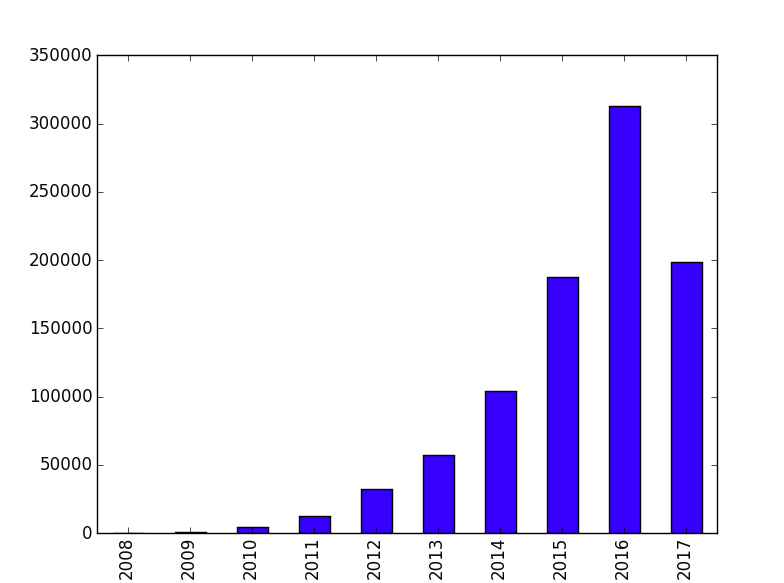
\includegraphics[width=10cm]{fig/fig1.png}
%
%\end{figure}
%
%
%\subsection{Analyse statistique}
%
%Plusieurs méthodes statistiques sont mobilisées afin d’analyser les données. Elles sont mises en %œuvre à l’aide de Python. Des statistiques descriptives sont mobilisées pour mettre en évidence %les modalités d’utilisation du réseau social. Les liens entre différentes variables sont testés à %l’aide de régressions multiples. Enfin, des tests non paramétriques sont utilisés pour comparer %différentes catégories de comptes (type d’entreprise, mission environnementale ou non). Le recours %à ce type de tests est imposé par la structure des données, qui ne respectent pas les conditions %d’application de tests paramétriques.
%
%\subsection{Analyse lexicale}
%Cette phase de l’étude s’intéresse plus précisément au sens des messages diffusés sur le réseau. %L’analyse lexicale permet d’étudier isolément les mots du corpus, c'est-à-dire détachés de leur %contexte. L’analyse repose sur la quantification des formes lexicales. L’étude s’appuie %spécifiquement sur les hashtags, c'est-à-dire les éléments du tweet mis en avant par l’émetteur du %message. Ce procédé n’est pas obligatoire, mais est mobilisé pour une proportion importante de %tweets (47.3\% du total des tweets collectés). L’étude utilise les hashtags pour déterminer le %cadre rhétorique dans lequel s’inscrit un message. Les cadres renvoient à la façon dont le %discours donne du sens à son objet. Comme le souligne \textcite{nisbet2009communicating}, toute %information s’inscrit dans un cadre donné. Il identifie huit cadres utilisés dans la communication %sur le changement climatique, qui peuvent s’appliquer à l’ensemble des enjeux écologiques. Le  %tableau \ref{table:6} présente ces cadres et précise les modalités d’opérationnalisation.
%
%
%
%\begin{landscape}
%\begin{spacing}{1}
%\begin{small}
%    \begin{longtable}{|K{0.18\linewidth}|K{0.38\linewidth}|K{0.40\linewidth}|}
%        \caption{Typologie des cadres du discours}
%        \label{table:6} \\
%            \hline
%            \textbf{Cadre} & \textbf{Définition \parencite{nisbet2009communicating} \newline %Frames define science-related issue as…} & \textbf{Opérationnalisation}\\ \hline
%            \endfirsthead
%            \hline
%            \textbf{Cadre} & \textbf{Définition \parencite{nisbet2009communicating}} & %\textbf{Opérationnalisation}\\ \hline
%            \endhead
%            \hline
%                Progrès Social
%                &A means of improving quality of life or solving problems; alternative %interpretation as a way to be in harmony with nature instead of mastering it.
%                &Le cadre est élargi aux hashtags qui renvoient à des questions d’ordre sociétal
%                \\ \hline
%
%                Développement économique et compétitivité
%                &An economic investment; market benefit or risk; or a point of local, national, or %global competitiveness.
%                &Le cadre intègre tous les hashtags qui renvoient à des dimensions d’économie, %d’emploi, de compétitivité ou à la notion de marché
%                \\ \hline
%
%                Moralité et éthique
%                &A matter of right or wrong; or of respect or disrespect for limits, thresholds, %or boundaries.
%                &Le cadre intègre tous les hashtags renvoyant à la morale, à des valeurs sociales, %de respect ou de solidarité.
%                \\ \hline
%
%                Incertitude scientifique et technique
%                &A matter of expert understanding or consensus; a debate over what is known versus %unknown; or peer-reviewed, confirmed knowledge versus hype or alarmism.
%                &Hashtags renvoyant plus généralement à de questions techniques et scientifiques, %sans prise de position explicite
%                \\ \hline
%
%                Boîte de Pandore, Monstre de Frankenstein et ‘Sauve-qui-peut’
%                &A need for precaution or action in face of possible catastrophe and %out-of-control consequences; or alternatively as fatalism, where there is no way %to avoid the consequences or chosen path.
%                &Hashtags renvoyant à une dimension dramatique, focalisé sur les dangers et les %risques liés à la non prise en compte de l’environnement, ainsi que les %conséquences déjà observés
%                \\ \hline
%
%                Responsabilité publique et gouvernance
%                &Research or policy either in the public interest or serving special interests, %emphasizing issues of control, transparency, participation, responsiveness, or %ownership; or debate over proper use of science and expertise in decisionmaking %(“politicization”).
%                &Hashtags renvoyant à la gouvernance aussi bien au niveau des entreprises que des %institutions publiques, ainsi que les hashtags renvoyant à une responsabilité %partagée, citoyenne
%                \\ \hline
%
%                Alternatives et compromis
%                &A third way between conflicting or polarized views or options.
%                &Hashtags renvoyant à des alternatives, des exemples d’innovations, ou plus %généralement un changement, une transition
%                \\ \hline
%
%                Conflits et stratégies
%                &A game among elites, such as who is winning or losing the debate; or a battle of %personalities or groups (usually a journalist-driven interpretation).
%                &Hashtags renvoyant à des acteurs du débat public, à des lieux d’échange et de %constitution de stratégies, ou à des prises de position claires
%                \\ \hline
%
%
%    \end{longtable}
%\end{small}
%\end{spacing}
%\end{landscape}
%
%
%
%Cette classification donne lieu à deux analyses :
%\begin{itemize}
%    \item	Une Analyse Factorielle des correspondances (AFC), qui permet de confronter les %différents modèles d’entreprises de l’ESS avec les cadres utilisés. Elle est réalisée à l’aide %du programme FactoMineR à partir d’une table de contingence créée par un script Python ;
%    \item	Des tests non paramétriques de comparaison de moyenne. Ils visent à déterminer si le %nombre de de retweets ou de favoris est significativement plus important pour certaines %catégories.
%\end{itemize}
%
%\subsection{Visualisation à l’aide des réseaux}
%
%Des données relatives aux liens entre les organisations du panel sont collectées. A l’aide du %logiciel Gephi, elles permettent d’identifier des communautés d’utilisateurs interconnectés. Le %logiciel permet également de produire des visualisations du réseau constitué par les %organisations. Celles-ci viennent compléter les résultats et montrer comment les \aess\ %s’organisent et interagissent sur le réseau social Twitter.


\section{Etude du discours sur Twitter : précisions méthodologiques}

\subsection{Constitution du panel de comptes Twitter.}

\subsubsection{Sélection des comptes d’utilisateurs}

Deux méthodes sont utilisées conjointement pour constituer la liste.

Dans un premier temps, des entreprises de l’ESS sont identifiées à partir de sources institutionnelles. Lorsqu’elles possèdent un compte Twitter, celui-ci est ajouté aux abonnements. Les listes mobilisées proviennent du CNCRES, de l’ACP ou de la base ‘open data’ du gouvernement :
\begin{itemize}
    \item Liste des 100 principales coopératives (CNCRES)
    \item Liste des sociétés commerciales de l’ESS (\url{http://liste-entreprises.cncres.org/})
    \item Liste des associations reconnues d’utilité publique (data.gouv)
    \item Liste des fondations reconnues d’utilité publique (data.gouv)
    \item Liste des mutuelles (ACP)
\end{itemize}

Pour les deux premières, l’ensemble des entreprises a été traité ; pour les trois suivantes, étant donné le nombre considérable d’entreprises, une sélection aléatoire a été effectuée. Cette première approche nous garantit l’intégration d’une grande variété d’entreprises à l’échantillon.

La seconde approche se fait directement dans l’interface web de twitter et s’appuie sur des recherches et suggestions. Une recherche sur des mots clés renvoyant aux \eess (‘coopérative’, ‘socent’, ‘association’, etc.) a permis d’identifier les comptes d’entreprises de l’ESS ayant la meilleure visibilité. Les comptes pertinents pour la recherche ont été ajoutés aux abonnements. L’algorithme de Twitter propose des suggestions de comptes en lien avec les utilisateurs auxquels le compte est déjà abonné. Ces comptes suggérés sont étudiés au cas par cas afin de déterminer s’ils peuvent être ajoutés au panel. Cette méthode est répétée de manière itérative (les suggestions étant actualisées à chaque nouvel abonnement) et permet un effet \cit{boule de neige}. Une limite notable de cette méthode est qu’elle fonctionne \cit{en circuit fermé} : elle permet d’identifier uniquement des comptes connectés entre eux. Toutefois, la sélection aléatoire réalisée dans l’étape 1 garantit une certaine ouverture dans ces suggestions.

Le choix d’intégrer un compte à la liste est fait en se basant sur la description de l’utilisateur ou, le cas échéant, sur le site internet de l’entreprise. Les comptes ajoutés à la liste sont les suivants :
\begin{itemize}
    \item Comptes d’entreprises de l’ESS (association, coopérative, mutuelle, association, fondation, entreprise sociale, entreprise d’insertion…),
    \item Comptes d’organismes de représentation de l’ESS (CRESS, CGSCOP…),
    \item Comptes d’incubateurs d’entreprises dédiés à l’ESS,
    \item Comptes d’évènements liés à l’ESS (Le mois de l’ESS…),
    \item Comptes de marques d’entreprises de l’ESS.
\end{itemize}

Les comptes individuels (militants, étudiants, enseignants, chercheurs, dirigeants ou employés de l’ESS, responsables politiques en charge de l’ESS) et les comptes des médias dédiés à l’ESS ne sont pas intégrés à la liste. Ce choix est fait afin de centrer le corpus sur le discours en provenance des acteurs de l’ESS et non de personnes intéressées par ce secteur ou ayant une posture critique.

Seuls ont été pris en compte les utilisateurs dont la description et les messages sont en langue française (essentiellement des entreprises françaises, mais également belges et québécoises).

Les données relatives aux comptes évoluent régulièrement (description, nombre d’abonnements, nombre de tweets…). Une mise à jour de tous les comptes est effectuée à l’issue de la collecte des tweets et avant la réalisation des analyses afin d’avoir les données les plus récentes.

\subsubsection{Affectation à des catégories}

Les utilisateurs sont affectés à l’une des catégories suivantes : Association, Coopérative (dont SCP, SCIC, SCE, coopératives d’entreprises, coopératives d’usagers, coopératives bancaires, autres coopératives), Fondation, Fédération, Mutuelle, Entreprise sociale, Autre. Il faut souligner que cette répartition ne repose pas strictement sur la forme juridique des entreprises, mais davantage sur la présentation des entreprises. Ainsi, alors qu’on ne recense que 93 sociétés commerciales dans l’ESS fin 2016 \parencite{observatoire_national_de_leconomie_sociale_et_solidaire_france2017atlas}, l’échantillon comprend près de 72 \cit{entreprises sociales}. En réalité, de nombreuses entreprises adoptent un statut associatif ou coopératif, mais se définissent comme entreprise sociale. Au-delà du statut, ceci traduit une volonté de s’inscrire dans un courant et dans une démarche particulière. Pour cette raison, les associations, fondations ou coopératives qui se présentent explicitement comme des entreprises sociales dans leur description sont affectées à la catégorie \cit{entreprises sociales}. De mêmes la catégorie \cit{Fédération} ne constitue pas une forme juridique d’entreprise. Ce groupe est constitué de tous types d’entreprises qui ont pour spécificité de rassembler et de fédérer un réseau d’organisations. La catégorie \cit{autre} regroupe des comptes qui ne sont pas des comptes d’entreprises, mais des comptes correspondants à des marques, évènements ponctuels ou réseaux informels. Ainsi, la catégorisation réalisée ici n’a pas pour vocation à reproduire la répartition de l’ESS en différents statuts, mais plutôt à apporter des éléments d’analyse. Le statut juridique est utilisé comme critère d’affectation en l’absence d’éléments déclaratifs. Cette information est généralement disponible dans les mentions légales du site internet de l’organisation ou sur des annuaires d’entreprises en ligne.

\subsubsection{Détermination de la dimension environnementale de l’organisation}

Elle nécessite une analyse plus fine de l’organisation. Les critères suivants sont appliqués : \begin{itemize}
    \item Si l’organisation a une activité principale directement liée à l’environnement, elle est qualifiée d’organisation environnementale (OE) : la variable prend la valeur VRAIE.
    \item Si l’organisation a une activité principale non liée à l’environnement, la variable prend la valeur FAUX.
    \item si l’organisation a une activité principale indirectement liée à l’environnement, la valeur est VRAI uniquement si la dimension écologique est mise en avant dans la description du compte. Par exemple, une épicerie bio est considérée comme environnementale uniquement si elle indique que la démarche bio est adoptée pour des raisons écologiques. De même, une association de protection des animaux est considérée comme environnementale si la finalité est la préservation de l’écosystème.
\end{itemize}

Le Tableau \ref{table:exempleutilisateur} présente un exemple d’enregistrement correspondant à un compte Twitter d’une association.

\begin{table}[h]
    \caption{Exemple d'enregistrement - compte d'utilisateur}
    \label{table:exempleutilisateur}
    \begin{tabularx}{\linewidth}{|l|L|}
    \hline
        \textbf{rowid} & 96 \\ \hline
        \textbf{nom\_utilisateur}	& HabitatetHumani \\ \hline
        \textbf{id\_utilisateur} &	1111275763 \\ \hline
        \textbf{description}	& Depuis 30 ans, Habitat et Humanisme agit en faveur du logement et de l'insertion des personnes en difficulté. \\ \hline
        \textbf{nb\_abonnements}	& 117 \\ \hline
        \textbf{nb\_abonnes}	& 2114 \\ \hline
        \textbf{nb\_tweets}	& 1074 \\ \hline
        \textbf{nombre\_recherche} &	37 \\ \hline
        \textbf{fini} &	True \\ \hline
        \textbf{date\_maj} &	2017/11/04 \\ \hline
        \textbf{compte\_envir} &	False \\ \hline
        \textbf{type\_compte} &	Association \\ \hline
    \end{tabularx}

    \textit{Les champs ‘fini’ et ‘nombre\_recherche’ sont des champs techniques permettant au script de déterminer quel compte prioriser pour la collecte des tweets. }
\end{table}


\subsubsection{Relations entre les utilisateurs}
Deux méthodes distinctes sont utilisées pour déterminer les liens entre les utilisateurs et permettre l’analyse des communautés. La première s’appuie sur les relations d’abonnements / abonnés. Pour cela, nous avons collecté la liste des abonnements de chaque compte et retenu uniquement ceux appartenant au panel (les abonnements à des comptes ne faisant pas partie du panel ne sont pas pris en compte). Un script détermine si la relation est unidirectionnelle (A est abonné à B mais B n’est pas abonné à A) ou bidirectionnelle (A est abonné à B et réciproquement) (cf. Encadré \ref{encadre:abos}). Le calcul des communautés par Gephi prend en compte cette information : une relation bidirectionnelle est pondérée de façon à être plus \cit{forte} qu’une  relation unidirectionnelle, et un utilisateur ayant un grand nombre de relations unidirectionnelles entrantes (c'est-à-dire qu’il est suivi par des comptes auquel lui-même n’est pas abonné) aura un degré de centralité plus élevé. Il ressort donc mieux sur la visualisation produite. Pour les mentions, l’approche est un peu différente car elle ne s’appuie pas sur une variable binaire mais quantitative : A peut mentionner B plusieurs fois et réciproquement. Pour chaque mention, on crée une relation $A\Rightarrow B$ qui peut se répéter (cf. Encadré \ref{encadre:mentions}). Gephi détermine les communautés en fonction du nombre de relations entrantes et sortantes pour chaque utilisateur.

\begin{encadre}
    \caption{Extrait du fichier des relations par abonnement}
    \label{encadre:abos}
    \noindent\fbox{
        \parbox{\linewidth-2\fboxrule-2\fboxsep}{
            \texttt{
            \begin{small}
                Source,Target,Weight,Type \\
                MaxHavelaarFr,greenpeacefr,2,Undirected \\
                MaxHavelaarFr,ccfd\_tsolidaire,2,Undirected \\
                MaxHavelaarFr,oxfamfrance,2,Undirected \\
                oxfamfrance,Energie\_SolidR,2,Undirected \\
                oxfamfrance,AmisDEnercoop,2,Undirected \\
                oxfamfrance,Bloom\_FR,2,Undirected
                \end{small}
            }
        }
    }
\end{encadre}

\begin{encadre}
    \caption{Extrait du fichier des relations par mentions}
    \label{encadre:mentions}

    \noindent\fbox{
        \parbox{\linewidth-2\fboxrule-2\fboxsep}{
            \texttt{
                \begin{small}
        Source,Target \\
        RACFrance,RACFrance \\
        amisdelaterre,amisdelaterre \\
        greenpeacefr,RACFrance \\
        greenpeacefr,emmaus\_france \\
        greenpeacefr,Bloom\_FR \\
        greenpeacefr,RACFrance RACFrance,RACFrance \\
        amisdelaterre,amisdelaterre  \\
        greenpeacefr,RACFrance \\
        greenpeacefr,emmaus\_france  \\
        greenpeacefr,Bloom\_FR
            \end{small}
            }
        }
    }
\end{encadre}

\subsection{Modalités de collecte des tweets}

Twitter limite le nombre de tweets collectés à 200 par utilisateur et par requête. Par conséquent, un processus itératif a été déployé afin de collecter le plus grand nombre possible de tweets pour chaque utilisateur du panel. Les tweets les plus récents sont collectés en priorité, puis chaque itération recherche des tweets plus anciens, jusqu’à avoir collecté l’intégralité des tweets. Seuls les tweets visibles publiquement sont collectés. Les tweets supprimés ou postés par des utilisateurs ayant restreint l’accès à leur compte ne sont pas collectés.

Les informations sur le niveau d’attention obtenu par les tweets (nombre de retweets et nombre de favoris) sont collectés \textit{a posteriori} (au moins un mois après la publication du tweet le plus récent) afin d’attendre leur stabilisation. Un tweet va en effet recueillir le plus grand nombre de favori et de retweets  dans les heures et les jours suivant sa publication.


\begin{table}[h]
    \caption{Exemple d'enregistrement - tweet}
    \label{table:exempleenregistrement}
    \begin{tabularx}{\linewidth}{|l|L|}
    \hline
        \textbf{rowid}& 	197494 \\ \hline
        \textbf{tweet\_id} & 	794493862119178000 \\ \hline
        \textbf{auteur}	& LaKoncepterie \\ \hline
        \textbf{auteur\_id}	& 3936984087 \\ \hline
        \textbf{date}	& 2016-11-04 10:57:52.000000 \\ \hline
        \textbf{mois}	& 11 \\ \hline
        \textbf{annee}	& 2016 \\ \hline
        \textbf{texte}	& L. Metivet d'@insereco93: \#humain, \#environnemental, l'\#ESS crée de nouveaux \#métiers \#EstplorationPositive \#ESS @seinesaintdenis \#insertion \\ \hline
        \textbf{retweet}	& False \\ \hline
        \textbf{hashtags}	& humain, environnemental, ESS, métiers, EstplorationPositive, ESS, insertion \\ \hline
        \textbf{active}	& True \\ \hline
    \end{tabularx}
    \textit{Le champ active permet d’éliminer du corpus certains tweets correspondant à du spam. }
\end{table}

\subsection{Préparation des données}

\subsubsection{Détermination du caractère environnemental d’un tweet}
L’étude s’intéresse uniquement aux tweets qui traitent de questions environnementales. Il est donc nécessaire de déterminer des critères permettant de filtrer les tweets en lien avec cette thématique. Trois critères sont utilisés.
\begin{itemize}
    \item Le premier critère retient tous les tweets évoquant directement « l’environnement » ou « l’écologie ». Il s’agit des contenus comportant un mot ayant la racine ‘environn’ ou ‘écolo’.
    \item Le second critère est plus ouvert. Parmi les 3000 hashtags les plus couramment utilisés dans le corpus de tweets, 101 hashtags relatifs à la question environnementale ont été identifiés (cf. Encadré \ref{encadre:htenvir}). Tous les tweets utilisant un de ces hashtags sont retenus.
    \item Le critère 3 retient tous les tweets ayant un caractère environnemental selon l’un des deux critères précédents. C’est le critère qui est retenu pour l’ensemble de l’étude.
\end{itemize}

\begin{encadre}
    \caption{principaux hashtags relatifs à l'environnement}
    \label{encadre:htenvir}

    \noindent\fbox{
        \parbox{\linewidth-2\fboxrule-2\fboxsep}{
            \texttt{
            \begin{small}
        accorddeparis, agroecologie, agroécologie, antigaspi, ateliercoecolo, bio, biocentrisme, biodéchets, biodiversite, biodiversité, changementclimatique, changerclimats, charbon, circuitcourt, circuitscourts, climat, climatdatalab, climatechange, climatgeopolble, climatique, confenvi, cop21, cop21paris, dd, déchet, dechets, déchets, deforestation, déforestation, devdurable, developpementdurable, développementdurable, durable, eco, ecocollab, écolo, ecologie, écologie, écologique, economiecirculaire, économiecirculaire, emballages, énergétique, energie, énergie, energiecitoyenne, énergies, energiesrenouvelables, environment, environnement, environnementale, éolien, foret, forêt, forêts, gazdeschiste, gocop21, greenwashing, huiledepalme, loibiodiv, loup, loups, nature, naturealert, nucleaire, nucléaire, obsolescenceprogrammée, oceanclimax, ogm, ouiauxloups, pêcheprofonde, permaculture, pesticides, petitionpesticides, pétrole, photovoltaique, photovoltaïque, plantfortheplanet, pollution, pollutionair, pollutiondelair, projectrescueocean, recyclage, recycler, recyclivredays, réemploi, renouvelable, renouvelables, rénovationénergétique, sosloups, stopcharbon, stopdeforestation, stoppesticides, transitionecologique, transitionenergetique, transitionenergétique, transitionénergétique, zerodechet, zérodéchet, zérodéforestation, zerowaste
            \end{small}
            }
        }
    }
\end{encadre}



\subsubsection{Elimination des tweets répétés}
Des tweets identiques ou très similaires peuvent affecter les résultats en donnant un poids trop important à une thématique portée par un seul utilisateur. Il peut s’agir de spam (organisation qui republie très régulièrement un lien vers son site internet) avec le même texte d’accompagnement ou d’une communication normale. C’est le cas de l’association Airparif qui informe quotidiennement les franciliens du niveau de pollution sous le format suivant :\cit{ La \#pollution en Île-de-France sera faible aujourd'hui (indice 46/100) et faible demain (37/100). https://t.co/uFdy5tXBv1}. Ces tweets sont donc écartés de l’analyse.

\subsubsection{Retraitement du texte}
Notre étude adopte l’approche de la statistique lexicale pour laquelle l’unité d’analyse est le mot. Celle-ci nécessite un nettoyage préalable des données afin :
\begin{itemize}
    \item De supprimer les mots non porteurs de sens (prépositions, démonstratifs, dates…)
    \item De regrouper les mots ayant la même racine mais une forme grammaticale différente
\end{itemize}
Nous avons procédé de la façon suivante. Chaque tweet est considéré comme un \cit{sac de mots} (approche \textit{bag of words}). Le module \textit{TreeTaggerWrapper} est utilisé pour associer chaque mot à sa forme grammaticale. Les mots identifiés comme adverbes, articles définis, pronoms possessifs, conjonctions, nombres, pronoms, pronoms démonstratifs, pronoms indéfinis, pronoms personnels, pronoms relatifs, prépositions ou symboles sont éliminés. On procède ensuite à une phase de lemmatisation, à l’aide du même module : chaque forme d’un mot est ramené à son lemme (par exemple, un verbe conjugué est ramené à l’infinitif, un mot au féminin est ramené au masculin etc.). Un exemple est donné dans le Tableau \ref{table:exempletraitement}.

\begin{table}[h]
    \caption{Exemples de retraitement d'un tweet}
    \label{table:exempletraitement}
    \begin{tabularx}{\linewidth}{|L|L|}
    \hline
      \textbf{  Tweet original}	& \textbf{Tweet retraité }\\ \hline
        Stop aux idées reçues! Et si on reconsidérait un peu le papier?
        \#RSE \#print \#papier \#communication \#environnement… https://t.co/KXp6gytt0b
        & stop idée reçu ! reconsidérer papier ? \# rse \# print \# papier \# communication \# environnement url-remplacée. \\ \hline

        .@Veillerette "le maintien d'une Europe forte sur les programme \#santé \#environnement est importante
        & @ veillerette maintien europe fort programme \# santé \# environnement être important \\ \hline
    \end{tabularx}
\end{table}

Pour la classification non supervisée, on élimine également la ponctuation, les symboles tels que ‘\#’ et les urls qui n’apportent pas de sens aux thématiques générées.


\subsection{Précisions sur les analyses réalisées}

\subsubsection{Classification non supervisée}
Deux algorithmes sont utilisés pour cette phase de l’étude : \textit{Latent Dirichlet Allocation} (LDA) et NMF. Pour le modèle NMF, deux implémentations sont testées, l’une suivant la norme de Frobenius, l’autre selon la divergence de Kullback-Leibler. On ne s’intéresse pas ici aux fondements probabilistes de ces approches : on se contentera de comparer les résultats et de déterminer ceux qui aboutissent à des catégories porteuses de sens.

Pour ces deux algorithmes, le nombre de catégories souhaitées doit être choisi a priori. Or, l’objectif de l’exploration de texte étant de « découvrir » ces catégories, leur nombre n’est pas connu du chercheur. Nous avons procédé par tests successifs avec des valeurs comprises entre 4 et 10 catégories. La valeur optimale est atteinte lorsque tous les groupes formés sont bien distincts et clairement identifiables.

\subsubsection{Classification supervisée}
L’algorithme de Naives-Bayes est utilisé pour la classification supervisée selon deux critères : le sentiment et l’objectivité. 430 tweets sont codés manuellement pour la phase d’entraînement. Ils sont répartis en quatre fichiers de la manière suivante :
\begin{itemize}
    \item 125 tweets négatifs – 305 tweets positifs,
    \item 147 tweets objectifs – 283 tweets subjectifs
\end{itemize}

Pour chaque fichier, 80 \% des tweets sont utilisés pour l’apprentissage et les 20 \% restants pour tester l’algorithme. Le programme effectue l’entraînement sur le premier lot, puis applique l’algorithme sur les 20 \% restants. La catégorie affectée par le programme est ensuite comparée à celle affectée par le chercheur. La validité est déterminée par le pourcentage de tweets pour lesquels le programme aboutit à la même catégorie que le chercheur. A l’issue de la phase d’entraînement, l’algorithme est appliqué sur l’intégralité des tweets.
Nous calculons ensuite le nombre de tweets pour chaque catégorie afin de déterminer la stratégie rhétorique la plus commune. Nous comparons également la performance de chaque stratégie en comparant les tweets de chaque groupe selon trois indicateurs : le nombre de retweets, le nombre de favoris et le niveau d’engagement. Ce dernier indicateur permet de contrôler l’effet du nombre d’abonnés, qui est très positivement associé à l’attention obtenue par un tweet. Il est construit de la façon suivante : \\

$ \text{Engagement} = \dfrac{\text{Nombre de retweets} + \text{Nombre de favoris}}{\text{Nombre d'abonnés}} \times 10000 $

\section{Informations techniques - outils utilisés}

\subsection{Python}
La collecte, le traitement, et la majorité des analyses sont effectués avec Python 3.6 (\url{https://www.python.org}). Les scripts ont été intégralement écrits par l’auteur, à l’aide des nombreuses ressources disponibles en ligne (formelles ou anonymes), notamment :
\begin{itemize}
    \item Des tutoriels mis à disposition par Gregory Saxton et Weiai Wayne Xu pour la collecte des tweets \parencite{saxtonnodatesocial, xunodatesignificant}
    \item Du modèle de script proposé par Olivier Grisel, Lars Buitinck et Chyi-Kwei Yau pour la classification non supervisée (\url{https://tinyurl.com/y79k8mxh})
    \item Des nombreux conseils et réponses apportés par les utilisateurs du site \url{https://stackoverflow.com/}.
\end{itemize}

Les données collectées sont stockées dans une base de données au format SQLite. Toutes les opérations effectuées sur la base de données sont effectuées via des scripts Python et sont ainsi documentées précisément.

Le langage Python s’appuie sur de nombreux modules librement accessibles et destinés à des opérations précises. Nous avons utilisé les modules suivants :
\begin{itemize}
    \item Twython pour l’accès aux données Twitter (\url{https://twython.readthedocs.io/en/latest/#usage})
    \item SQLAlchemy pour l’utilisation de la base de données (\url{https://www.sqlalchemy.org/})
    \item Django pour la création d’une interface utilisateur pour collecter les données (\url{https://www.djangoproject.com/}).
    \item NLTK pour le traitement des données lexicales et la mise en œuvre de l’algorithme de Naives-Bayes \parencite{bird2009natural}.
    \item TreeTagger et TreeTaggerWrapper pour le retraitement du texte (part of speech tagging) \parencite{schmid1994probabilistic, schmid1995improvements}.
    \item Modules de l’écosystème SciPy destiné à l’usage scientifique de Python : Pandas, NumPy, scikit-learn, Matplotlib \parencite{hunter2007matplotlib:, jones2001scipy:, mckinney2010data, oliphant2007python, pedregosa2011scikit-learn:}.
    \item Statsmodels pour les regressions linéaires \parencite{seabold2010statsmodels:}.
\end{itemize}


\subsection{Autres outils}

Pour la représentation visuelle du réseau d’utilisateur, le logiciel libre et open-source Gephi a été utilisé (\url{https://gephi.org/}).

L’analyse factorielle des correspondances a été réalisée avec le langage R et du package FactoMineR qui constitue un outil très puissant pour l’analyse factorielle \parencite{le2008factominer} .

          \chapter{Questionnaire de recherche}
            \label{annexe:guide}
\section*{Introduction}
    \textbf{Présentation du chercheur et du contexte de la recherche}
    \begin{itemize}
        \item Recherche menée à Aix-Marseille Université dans le cadre d’une thèse en gestion des organisations.  
        \item Travail sur la prise en compte de l’environnement dans l’ESS
        \item Retour sur les entretiens à l’issue de l’analyse et avant la soutenance de thèse (prévoir un délai d’un an) \\
    \end{itemize}
    	
    \textbf{Objectifs de l’entretien : }
        \begin{itemize}
            \item Comprendre le fonctionnement de votre entreprise.
            \item Comprendre ce qui motive ou freine vos décisions en matière environnementale. \\
        \end{itemize}
        

    \textbf{Les principes : } \\
        Posture d’un entretien de recherche  assez codifié : 
            \begin{itemize}
                \item Questions ouvertes, possible d’extrapoler. Les questions ne servent qu’à guider l’entretien.
                \item Ne pas hésiter à expliquer des choses qui peuvent paraître évidentes (pour avoir votre point de vue).
                \item Positionnement neutre : pas de jugement, pas de bonne ou mauvaise réponse. Pas de prise de position du chercheur pendant l’entretien, mais possible d’avoir un échange à la fin de l’entretien.  \\
            \end{itemize}
        L’entretien est enregistré, cependant l’anonymat est garanti. Il est possible d’interrompre l’enregistrement à votre demande si un sujet confidentiel est abordé. Le nom de personnes éventuellement citées pendant l’entretien sera changé dans la retranscription.

        
\section*{Présentation de l’entreprise et du répondant }
Pouvez-vous me parler de votre organisation/entreprise ? 
    \begin{itemize}
    	\item Quel est le statut juridique de votre organisation/entreprise ? 
    	\item Effectif, année de création, initiative de la création ? \\
	\end{itemize} 

Pouvez-vous me parler de votre position, votre rôle dans l’organisation/entreprise ? \\

Comment décririez-vous la mission de votre organisation/entreprise ?  
    \begin{itemize}
        \item Quelles sont ses activités principales ? A qui s’adressent-elles ? 
        \item Qui sont vos client / bénéficiaires ? Ont-ils un statut particulier (adhérent…)
        \item Quel type d’impact cherchez-vous à avoir ? (social, environnemental, économique) \\
    \end{itemize}
	
Quel est votre périmètre d’action ? (local / national / international) 

\section*{Caractéristique de l’organisation/entreprise}
Qui sont vos employés ? 
\begin{itemize}
    \item Bénévoles / salariés
    \item Type de contrats  \\
\end{itemize}

A qui appartient l’organisation/entreprise et qui la dirige ?
    \begin{itemize}
        \item Structure du groupe et lien mère-filiales ?
        \item Comment et par qui sont prises les décisions ? 
        \item Structure centralisée / décentralisée ? 
        \item Organisation verticale ou horizontale ? (hiérarchie)
        \item Qui est représenté au conseil d’administration ?  \\
    \end{itemize}

Vous appuyez vous sur des partenariats ? 
\begin{itemize}
    \item Qui sont vos partenaires clés ? 
    \item Sur quelles bases reposent ces partenariats ? 
    \item Quel intérêt avez-vous dans ces partenariats ? 
    \item Que leur apportez-vous ? 
    \item Quelle importance donnez-vous à ces partenariats ?  \\
\end{itemize}
	
Quelles sont les sources de revenus de votre organisation/entreprise ? (Dons d’entreprises ? de particuliers ? Mécénat ? Subventions ? Chiffre d’affaires ? Revenus publicitaires ?)
    \begin{itemize}
        \item Revenus réguliers ou irréguliers ? 
        \item D’où viennent les capitaux ? (Capital social, crédit, investissement solidaire…) \\
    \end{itemize}

Quels sont les principaux postes de dépense ? 

Êtes vous en concurrence avec d’autres organisations, et comment vous situez vous dans cette concurrence ? 
    \begin{itemize}
        \item En termes de prix ? 
        \item Parts de marché ? 
        \item Logique de domination de marché, de masse ?  \\
    \end{itemize}
	
Est-ce que vous évaluez les résultats de votre organisation/entreprise ? 
    \begin{itemize}
        \item Sur quels critères ? \\
    \end{itemize}

Comment décririez-vous les valeurs de votre organisation/entreprise ? 
    \begin{itemize}
        \item Qu’est ce qui est le plus important pour vous ? \\
    \end{itemize}

Quelles sont les perspectives et projets de votre organisation/entreprise ? 
    \begin{itemize}
        \item Croissance ? 
        \item Nouveaux marchés ? 
        \item Nouvelles actions ?
        \item Etc. \\
    \end{itemize}
	
Avez-vous le sentiment d’appartenir à l’ESS ? 
    \begin{itemize}
        \item Qu’est ce que ça veut dire pour vous ? 
        \item Est-ce que cela vous semble important ? 
        \item Qu’est ce qui vous y rattache le plus ? 
        \item Qu’est ce que cela change pour vous ? \\
    \end{itemize}

\section*{Innovation environnementale}
Pensez-vous que l’activité d’une organisation comme la vôtre a un impact environnemental (direct ou indirect) ?
    \begin{itemize}
        \item Quel type d’impact ? 
        \item Êtes-vous soumis à des normes environnementales ? 
        \item (Si applicable : Au-delà de vos activités, votre fonctionnement a-t-il un impact ?) \\
    \end{itemize}

Avez-vous une stratégie / une réflexion sur ces sujets ?  
    \begin{itemize}
        \item Cette réflexion est-elle prioritaire ? \\
    \end{itemize}
	

Avez-vous déjà mené des actions dans une perspective environnementale ? 
    \begin{itemize}
        \item Ou avez-vous comme projet de mener de telles actions dans le futur ?  \\
    \end{itemize}
	

Ces actions ont-elles nécessité de mettre en place des adaptations, des changements, des innovations ? \\

Sur quoi ont porté ces actions ? 
    \begin{itemize}
        \item Sur les produits et services ?
        \item Sur l’organisation ? 
        \item Rapport au consommateur ?  
        \item Systèmes de management ? Procédures ? Certifications ?  \\
    \end{itemize}


S’agissait-il plutôt d’adaptations de l’existant ou de l’introduction de quelque chose de complètement nouveau pour vous ? \\

Qu’est-ce qui vous a poussé à réaliser ces innovations avec un impact environnemental ? 
    \begin{itemize}
        \item Recherche de rentabilité
        \item Demande du client 
        \item Amélioration de l’offre
        \item Evolution légale 
        \item ... \\
    \end{itemize}

Avez-vous rencontré des obstacles à la mise en œuvre de ces innovations ? 
    \begin{itemize}
        \item Financiers
        \item Organisationnels
        \item Humains
        \item ... \\
    \end{itemize}
    
Au contraire, qu’est-ce qui a facilité la mise en œuvre de ces innovations ? 
    \begin{itemize}
        \item Organisation
        \item Partenariats
        \item Humains \\
    \end{itemize}

Quels effets attendiez-vous de ces innovations ?
    \begin{itemize}
        \item Avez-vous obtenu les résultats escomptés ? 
        \item Avez-vous évalué l’impact de ces innovations ? \\
    \end{itemize}
	
	

Qu’est-ce qui a guidé votre choix vers certaines innovations plutôt que d’autres ? \\ 

Pensez-vous qu’appartenir à l’ESS soit un atout pour mettre en œuvre des innovations en lien avec l’environnement ? \\

Avez-vous de nouveaux projets d’innovations en lien avec l’environnement ?  \\

Avez-vous des documents relatifs à votre organisation/entreprise (rapports annuels) et à votre action environnementale (rapports RSE…) \\

\section*{Conclusion}
Principaux points abordés \\

Souhaitez-vous ajouter quelque chose ? \\

Remerciements 

        \end{appendices}

%----------------------------------------------------------------------------------------
%	BACKMATTER - résumé et abstract
%----------------------------------------------------------------------------------------

\backmatter
    %%Résumé et abstract
    		\chapter*{Résumé}
    		\markboth{Résumé}{}
    		\addstarredchapter{Résumé}
    		% SET SPECIFIC FONT
\usefont{T1}{phv}{m}{n}\selectfont{}
\renewcommand*{\arraystretch}{1.2}


\begin{center}
  \large \textbf{Les organisations de l'Économie Sociale et Solidaire face aux enjeux écologiques : stratégies de communication et d'action environnementale}
\end{center}

\vspace{1cm}

La protection de l'environnement naturel constitue un enjeu déterminant pour le futur de l'humanité. L'Économie Sociale et Solidaire (ESS), qui partage les principes du développement durable, est particulièrement bien placée pour mettre en oeuvre des alternatives de développement plus écologiques. Ce secteur composé des associations, des coopératives, des mutuelles, des fondations et des entreprises sociales bénéficie d'un préjugé positif puisque ses organisations agissent pour l'intérêt général. C'est pourquoi peu d'attention est donnée à l'action environnementale de ces organisations. Cette recherche a pour objet d'examiner les facteurs et les modalités de l'action environnementale dans cette économie hétérogène. La thèse appréhende les organisations de l'ESS sous l'angle de l'identité organisationnelle et s'intéresse d'une part à la communication environnementale, d'autre part aux actions concrètes. Une étude est menée pour chacun de ces deux volets de la recherche.\\

La première étude a pour terrain le réseau social Twitter et vise à identifier les stratégies rhétoriques adoptées par les organisation de l'ESS sur les sujets liés à l'environnement. Plus de 910 000 tweets ont été collectés et analysés à l'aide d'un programme codé dans le langage information Python. En recourant à une démarche \citit{Big-Data} et à l'aide des techniques d'exploration automatique de texte, nous identifions les principales thématiques du corpus et mettons en évidence l'opposition entre des stratégies militantes et des stratégies basées sur les opportunités de développement économique. \\

Cette première étude est complétée par l'étude de sept cas, sur la base d'entretiens menés auprès de dirigeantes et dirigeants d'organisations de l'ESS. Elle s'intéresse aux facteurs de l'action environnementale, en lien avec l'identité organisationnelle de l'ESS. Les résultats mettent en lumière la grande diversité d'approches au sein de l'ESS, mais aussi le rôle déterminant de l'engagement individuel, des convictions et des logiques collectives dans la réalisation d'actions environnementale. L'étude aboutit à la formulation de huit propositions de recherche qui synthétisent les relations identifiées. \\

Ce travail apporte plusieurs contributions à la littérature. Sur le plan méthodologique, nous développons l'approche de l'exploration automatique de texte, rarement utilisée dans les Sciences de Gestion. Sur le plan théorique, la thèse introduit la dimension collective en tant qu'identité organisationnelle de l'ESS. Nous adaptons ensuite un modèle d'action environnementale en identifiant un déterminant supplémentaire spécifique à ces organisations. Finalement, la recherche invite l'ESS à remettre au centre les questions d'écologi, et donne des pistes pour soutenir les organisations dans une démarche environnementale. \\

\vspace{1cm}


\textit{\textbf{Mots clés :} Action environnementale, Économie Sociale et Solidaire, Rhétorique environnementale, Identité organisationnelle, Big-Data, Exploration de texte}


    		
    		%\addcontentsline{toc}{chapter}{Résumé}

        %% abstract
             
    		\chapter*{Abstract}
    		\markboth{Abstract}{}
    		\addstarredchapter{Abstract}
    		\begin{center}
  \large \textbf{Social and Solidarity Economy organisations in the face of ecological challenges: strategies for communication and environmental action}
\end{center}

\vspace{1cm}

The protection of the natural environment is a key stake for the future of humanity.  The Social and Solidarity Economy (SSE), which shares the principles of sustainable development, is particularly well placed to implement more ecological development options. This sector, which is composed of associations, cooperatives, mutual firms, foundations and social enterprises benefits from a positive bias since its organisations act in the general interest. As a result, little attention is paid to the environmental action of these organisations.
The purpose of this research is to examine the factors and modalities of environmental action in this heterogeneous economy. The thesis looks at SSE entities from the perspective of organizational identity, and focuses on environmental communication on the one hand, and concrete actions on the other. A study is conducted for each of these aspects.\\

The first study focuses on the Twitter social network and aims at identifying the rhetorical strategies adopted by SSE organisations on environment-related topics. More than 910,000 tweets were collected and analyzed with the help of a program coded in the Python information language. By applying a "Big-Data" approach as well as text mining techniques, we identify the main themes of the corpus, and highlight the opposition between militant strategies and strategies based on economic development opportunities. \\

This first study is completed by the examination of seven cases, based on interviews with leaders of SSE organisations. It focuses on the factors of environmental action, in relation to the organizational identity of the SSE. The results highlight the great diversity of approaches within the SSE, but also the decisive role of individual commitment, convictions and collective logic in the implementation of environmental actions. The study resulted in the formulation of eight research proposals that describe the identified relationships.  \\

This work makes several contributions to the literature. On the methodological level, we develop the text mining techniques, rarely used in Management Sciences. On the theoretical level, the thesis introduces the collective dimension as an organisational identity of the SSE. We then adapt an environmental action model by identifying an additional determinant specific to these organizations. Finally, the research invites the SSE to put ecological issues back at the centre, and provides suggestions for supporting organisations in an environmental approach.\\ 

\vspace{1cm}

\textit{\textbf{Mots clés :} Environmental action, Social and Solidary Economy, Environmental rhetoric, Organisational identity, Big-Data, Text-mining}

% RESET FONT
\usefont{T1}{bch}{m}{n}\selectfont{}
\renewcommand*{\arraystretch}{1.5}

    		
    		%\addcontentsline{toc}{chapter}{Abstract}

    %% TABLE DES MATIERES détaillée
    		\newpage
    		%\chapter*{Table des matières détaillée}
    		\addstarredchapter{Table des matières détaillée}
    		%\addcontentsline{toc}{chapter}{Table des matières détaillée}
    		\tableofcontents

\end{document}
